We have implemented our approach in a prototype and compared it with the related 
approaches refinepoly~\cite{refinepoly}, deepSRGR~\cite{deepsrgr} and deeppoly~\cite{deeppoly}. We also compare 
our tool with state of the art tools $\alpha - \beta$-Crown~\cite{alphabetacrown} and oval~\cite{ovaltool}. 
The $\alpha - \beta$-Crown tool has achieved the 1st and oval 3rd rank in
2nd International Verification of Neural Networks Competition (VNN-COMP'21). 
We use the MNIST \cite{mnistdataset} for our evaluation.    
\subsection{Implementation}
We have implemented our tool in \texttt{C++} programming language. Our approach relies on \deeppoly{}, so, 
we also have implemented \deeppoly{} in \texttt{C++}. We are using \texttt{C++} interface of gurobi solver 
to check the satisfiability or to solve an optimization query. 

\subsection{Benchmarks}
We are using the MNIST~\cite{mnistdataset} dataset to check the effectiveness of our tool. 
We are using 11 different fully connected feedforward neural networks with \relu{} activation as shown in table~\ref{tb:nndetail}.
These benchmarks are taken from the \deeppoly{}'s website~\cite{erantool}. The input and output dimensions of each network 
are $784$ and $10$ respectively. Deep et al~\cite{deeppolyref} used projected gradient descent (PGD)~\cite{pgdref}
and DiffAI~\cite{diffairef} for adversarial training. The table \ref{tb:nndetail} contains the defended network i.e.
trained with adversarial training as well as undefended network. The last column of the table \ref{tb:nndetail}
shows tools name by which the defended networks are trained.  

The predicate $P$ on input layer is computed using the input image $\boldsymbol{im}$ and user defined parameter $\epsilon$. 
We first normalize each pixel of $\boldsymbol{im}$ between $0$ and $1$, then create 
$P = \Land_{i=1}^{|l_0|} im(i)-\epsilon \leq x_{0i}\leq im(i)+\epsilon$, such that the lower and upper bound of each pixel
should not exceed $0$ and $1$ respectively. The predicate $Q$ on output layer is created using the network's output.    
Suppose the predicted label of $\boldsymbol{im}$ on network $N$ is $y$, then $Q = \Land_{i=1}^{|l_k|} x_{ki} < y$, where $i \neq y$. 
One query instance $\langle N,P,Q \rangle$ is created for one network, one image and one epsilon value. 
In our evaluation we took $11$ different networks, 8 different epsilons and 100 different images. The 
total number of instances are computed to $8800$. Whenever our tool found a counter example on $\langle N,P,Q \rangle$,
it denormalize it into an image by rounding the float values, 
and check for counter example by executing $N$ on denormalized image.
If found counter example then tool reports it, otherwise tool reports unknown.



\begin{table}
    \centering
    \begin{tabular}{c|c|c|c}
        \hline
        \textbf{Neural Network} & \textbf{\#hidden layers} & \textbf{\#activation units} & \textbf{Defensive training} \\
        \hline
        $3\times 50$ & 2 & 110 & None \\
        $3\times 100$ & 2 & 210 & None  \\
        $5\times 100$ & 4 & 410 & None  \\
        $6\times 100$ & 5 & 510 & DiffAI \\
        $9\times 100$ & 8 & 810 & None  \\
        $6\times 200$ & 5 & 1010 & None  \\
        $9\times 200$ & 8 & 1610 & None  \\
        $6\times 500$ & 6 & 3000 & None  \\
        $6\times 500$ & 6 & 3000 & PGD, $\epsilon = 0.1$ \\
        $6\times 500$ & 6 & 3000 & PGD, $\epsilon = 0.3$ \\
        $4\times 1024$ & 3 & 3072 & None  \\
        \hline
    \end{tabular}
    \caption{Neural networks details}
    \label{tb:nndetail}
\end{table}

\subsection{Results}
\begin{figure}
    \centering
    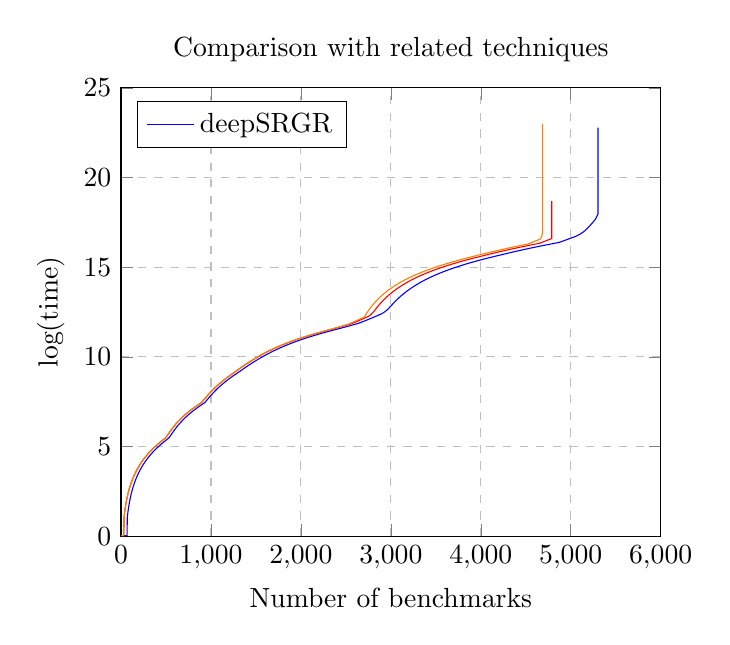
\begin{tikzpicture}
        \begin{axis}[
            title={Comparison with related techniques},
            xlabel={Number of benchmarks},
            ylabel={log(time)},
            xmin=0, xmax=6000,
            ymin=0, ymax=25,
            xtick={0,1000,2000,3000,4000,5000,6000},
            ytick={0,5,10,15,20,25},
            legend pos=north west,
            ymajorgrids=true,
            xmajorgrids=true,
            grid style=dashed,
        ]
        
        \addplot[
            color=blue
            ]
            coordinates {
                (1, 0.03)
                (2, 0.03)
                (3, 0.03)
                (4, 0.03)
                (5, 0.03)
                (6, 0.03)
                (7, 0.03)
                (8, 0.03)
                (9, 0.03)
                (10, 0.03)
                (11, 0.03)
                (12, 0.03)
                (13, 0.03)
                (14, 0.03)
                (15, 0.03)
                (16, 0.03)
                (17, 0.03)
                (18, 0.03)
                (19, 0.03)
                (20, 0.03)
                (21, 0.03)
                (22, 0.03)
                (23, 0.03)
                (24, 0.03)
                (25, 0.03)
                (26, 0.03)
                (27, 0.03)
                (28, 0.03)
                (29, 0.03)
                (30, 0.03)
                (31, 0.03)
                (32, 0.03)
                (33, 0.03)
                (34, 0.03)
                (35, 0.03)
                (36, 0.03)
                (37, 0.03)
                (38, 0.03)
                (39, 0.03)
                (40, 0.03)
                (41, 0.03)
                (42, 0.03)
                (43, 0.03)
                (44, 0.03)
                (45, 0.03)
                (46, 0.03)
                (47, 0.03)
                (48, 0.03)
                (49, 0.03)
                (50, 0.03)
                (51, 0.03)
                (52, 0.03)
                (53, 0.03)
                (54, 0.03)
                (55, 0.03)
                (56, 0.03)
                (57, 0.03)
                (58, 0.03)
                (59, 0.03)
                (60, 0.03)
                (61, 0.03)
                (62, 0.03)
                (63, 0.03)
                (64, 0.03)
                (65, 0.03)
                (66, 0.03)
                (67, 0.03)
                (68, 0.03)
                (69, 1.002)
                (70, 1.049)
                (71, 1.096)
                (72, 1.14)
                (73, 1.184)
                (74, 1.226)
                (75, 1.267)
                (76, 1.307)
                (77, 1.347)
                (78, 1.385)
                (79, 1.423)
                (80, 1.459)
                (81, 1.495)
                (82, 1.531)
                (83, 1.565)
                (84, 1.598)
                (85, 1.631)
                (86, 1.663)
                (87, 1.695)
                (88, 1.725)
                (89, 1.756)
                (90, 1.785)
                (91, 1.814)
                (92, 1.843)
                (93, 1.871)
                (94, 1.898)
                (95, 1.925)
                (96, 1.952)
                (97, 1.978)
                (98, 2.004)
                (99, 2.029)
                (100, 2.054)
                (101, 2.079)
                (102, 2.103)
                (103, 2.127)
                (104, 2.151)
                (105, 2.174)
                (106, 2.197)
                (107, 2.219)
                (108, 2.241)
                (109, 2.263)
                (110, 2.285)
                (111, 2.306)
                (112, 2.327)
                (113, 2.348)
                (114, 2.368)
                (115, 2.388)
                (116, 2.409)
                (117, 2.428)
                (118, 2.448)
                (119, 2.467)
                (120, 2.486)
                (121, 2.505)
                (122, 2.524)
                (123, 2.543)
                (124, 2.561)
                (125, 2.579)
                (126, 2.597)
                (127, 2.614)
                (128, 2.632)
                (129, 2.649)
                (130, 2.666)
                (131, 2.683)
                (132, 2.7)
                (133, 2.717)
                (134, 2.733)
                (135, 2.75)
                (136, 2.766)
                (137, 2.782)
                (138, 2.798)
                (139, 2.813)
                (140, 2.829)
                (141, 2.844)
                (142, 2.86)
                (143, 2.875)
                (144, 2.89)
                (145, 2.905)
                (146, 2.92)
                (147, 2.934)
                (148, 2.949)
                (149, 2.963)
                (150, 2.977)
                (151, 2.992)
                (152, 3.006)
                (153, 3.02)
                (154, 3.034)
                (155, 3.047)
                (156, 3.061)
                (157, 3.074)
                (158, 3.088)
                (159, 3.101)
                (160, 3.114)
                (161, 3.127)
                (162, 3.14)
                (163, 3.153)
                (164, 3.166)
                (165, 3.179)
                (166, 3.191)
                (167, 3.204)
                (168, 3.216)
                (169, 3.229)
                (170, 3.241)
                (171, 3.253)
                (172, 3.265)
                (173, 3.277)
                (174, 3.289)
                (175, 3.301)
                (176, 3.312)
                (177, 3.324)
                (178, 3.335)
                (179, 3.347)
                (180, 3.358)
                (181, 3.37)
                (182, 3.381)
                (183, 3.392)
                (184, 3.403)
                (185, 3.414)
                (186, 3.425)
                (187, 3.436)
                (188, 3.447)
                (189, 3.458)
                (190, 3.469)
                (191, 3.48)
                (192, 3.49)
                (193, 3.501)
                (194, 3.511)
                (195, 3.521)
                (196, 3.532)
                (197, 3.542)
                (198, 3.552)
                (199, 3.563)
                (200, 3.573)
                (201, 3.583)
                (202, 3.593)
                (203, 3.603)
                (204, 3.613)
                (205, 3.622)
                (206, 3.632)
                (207, 3.642)
                (208, 3.652)
                (209, 3.661)
                (210, 3.671)
                (211, 3.68)
                (212, 3.69)
                (213, 3.699)
                (214, 3.709)
                (215, 3.718)
                (216, 3.727)
                (217, 3.737)
                (218, 3.746)
                (219, 3.755)
                (220, 3.764)
                (221, 3.773)
                (222, 3.782)
                (223, 3.791)
                (224, 3.8)
                (225, 3.809)
                (226, 3.818)
                (227, 3.826)
                (228, 3.835)
                (229, 3.844)
                (230, 3.852)
                (231, 3.861)
                (232, 3.87)
                (233, 3.878)
                (234, 3.887)
                (235, 3.895)
                (236, 3.903)
                (237, 3.912)
                (238, 3.92)
                (239, 3.928)
                (240, 3.936)
                (241, 3.945)
                (242, 3.953)
                (243, 3.961)
                (244, 3.969)
                (245, 3.977)
                (246, 3.985)
                (247, 3.993)
                (248, 4.001)
                (249, 4.009)
                (250, 4.017)
                (251, 4.024)
                (252, 4.032)
                (253, 4.04)
                (254, 4.048)
                (255, 4.055)
                (256, 4.063)
                (257, 4.071)
                (258, 4.078)
                (259, 4.086)
                (260, 4.093)
                (261, 4.101)
                (262, 4.108)
                (263, 4.116)
                (264, 4.123)
                (265, 4.131)
                (266, 4.138)
                (267, 4.145)
                (268, 4.153)
                (269, 4.16)
                (270, 4.167)
                (271, 4.174)
                (272, 4.181)
                (273, 4.189)
                (274, 4.196)
                (275, 4.203)
                (276, 4.21)
                (277, 4.217)
                (278, 4.224)
                (279, 4.231)
                (280, 4.238)
                (281, 4.245)
                (282, 4.252)
                (283, 4.258)
                (284, 4.265)
                (285, 4.272)
                (286, 4.279)
                (287, 4.286)
                (288, 4.292)
                (289, 4.299)
                (290, 4.306)
                (291, 4.312)
                (292, 4.319)
                (293, 4.326)
                (294, 4.332)
                (295, 4.339)
                (296, 4.345)
                (297, 4.352)
                (298, 4.358)
                (299, 4.365)
                (300, 4.371)
                (301, 4.377)
                (302, 4.384)
                (303, 4.39)
                (304, 4.396)
                (305, 4.403)
                (306, 4.409)
                (307, 4.415)
                (308, 4.422)
                (309, 4.428)
                (310, 4.434)
                (311, 4.44)
                (312, 4.446)
                (313, 4.453)
                (314, 4.459)
                (315, 4.465)
                (316, 4.471)
                (317, 4.477)
                (318, 4.483)
                (319, 4.489)
                (320, 4.495)
                (321, 4.501)
                (322, 4.507)
                (323, 4.513)
                (324, 4.519)
                (325, 4.525)
                (326, 4.531)
                (327, 4.537)
                (328, 4.542)
                (329, 4.548)
                (330, 4.554)
                (331, 4.56)
                (332, 4.566)
                (333, 4.571)
                (334, 4.577)
                (335, 4.583)
                (336, 4.589)
                (337, 4.594)
                (338, 4.6)
                (339, 4.606)
                (340, 4.611)
                (341, 4.617)
                (342, 4.623)
                (343, 4.628)
                (344, 4.634)
                (345, 4.639)
                (346, 4.645)
                (347, 4.65)
                (348, 4.656)
                (349, 4.661)
                (350, 4.667)
                (351, 4.672)
                (352, 4.678)
                (353, 4.683)
                (354, 4.689)
                (355, 4.694)
                (356, 4.699)
                (357, 4.705)
                (358, 4.71)
                (359, 4.715)
                (360, 4.721)
                (361, 4.726)
                (362, 4.731)
                (363, 4.737)
                (364, 4.742)
                (365, 4.747)
                (366, 4.752)
                (367, 4.757)
                (368, 4.763)
                (369, 4.768)
                (370, 4.773)
                (371, 4.778)
                (372, 4.783)
                (373, 4.788)
                (374, 4.793)
                (375, 4.799)
                (376, 4.804)
                (377, 4.809)
                (378, 4.814)
                (379, 4.819)
                (380, 4.824)
                (381, 4.829)
                (382, 4.834)
                (383, 4.839)
                (384, 4.844)
                (385, 4.849)
                (386, 4.854)
                (387, 4.859)
                (388, 4.863)
                (389, 4.868)
                (390, 4.873)
                (391, 4.878)
                (392, 4.883)
                (393, 4.888)
                (394, 4.893)
                (395, 4.897)
                (396, 4.902)
                (397, 4.907)
                (398, 4.912)
                (399, 4.917)
                (400, 4.921)
                (401, 4.926)
                (402, 4.931)
                (403, 4.936)
                (404, 4.94)
                (405, 4.945)
                (406, 4.95)
                (407, 4.954)
                (408, 4.959)
                (409, 4.964)
                (410, 4.968)
                (411, 4.973)
                (412, 4.978)
                (413, 4.982)
                (414, 4.987)
                (415, 4.992)
                (416, 4.996)
                (417, 5.001)
                (418, 5.005)
                (419, 5.01)
                (420, 5.014)
                (421, 5.019)
                (422, 5.024)
                (423, 5.028)
                (424, 5.033)
                (425, 5.037)
                (426, 5.042)
                (427, 5.046)
                (428, 5.05)
                (429, 5.055)
                (430, 5.059)
                (431, 5.064)
                (432, 5.068)
                (433, 5.073)
                (434, 5.077)
                (435, 5.081)
                (436, 5.086)
                (437, 5.09)
                (438, 5.095)
                (439, 5.099)
                (440, 5.103)
                (441, 5.108)
                (442, 5.112)
                (443, 5.116)
                (444, 5.121)
                (445, 5.125)
                (446, 5.129)
                (447, 5.134)
                (448, 5.138)
                (449, 5.142)
                (450, 5.146)
                (451, 5.151)
                (452, 5.155)
                (453, 5.159)
                (454, 5.163)
                (455, 5.168)
                (456, 5.172)
                (457, 5.176)
                (458, 5.18)
                (459, 5.184)
                (460, 5.189)
                (461, 5.193)
                (462, 5.197)
                (463, 5.201)
                (464, 5.205)
                (465, 5.209)
                (466, 5.214)
                (467, 5.218)
                (468, 5.222)
                (469, 5.226)
                (470, 5.23)
                (471, 5.234)
                (472, 5.238)
                (473, 5.242)
                (474, 5.247)
                (475, 5.251)
                (476, 5.255)
                (477, 5.259)
                (478, 5.263)
                (479, 5.267)
                (480, 5.271)
                (481, 5.275)
                (482, 5.279)
                (483, 5.283)
                (484, 5.287)
                (485, 5.291)
                (486, 5.295)
                (487, 5.299)
                (488, 5.304)
                (489, 5.308)
                (490, 5.312)
                (491, 5.316)
                (492, 5.32)
                (493, 5.324)
                (494, 5.328)
                (495, 5.332)
                (496, 5.336)
                (497, 5.34)
                (498, 5.344)
                (499, 5.348)
                (500, 5.352)
                (501, 5.356)
                (502, 5.36)
                (503, 5.364)
                (504, 5.368)
                (505, 5.372)
                (506, 5.376)
                (507, 5.38)
                (508, 5.384)
                (509, 5.388)
                (510, 5.391)
                (511, 5.395)
                (512, 5.399)
                (513, 5.403)
                (514, 5.407)
                (515, 5.411)
                (516, 5.415)
                (517, 5.419)
                (518, 5.423)
                (519, 5.427)
                (520, 5.431)
                (521, 5.435)
                (522, 5.439)
                (523, 5.443)
                (524, 5.447)
                (525, 5.451)
                (526, 5.455)
                (527, 5.459)
                (528, 5.463)
                (529, 5.468)
                (530, 5.472)
                (531, 5.477)
                (532, 5.481)
                (533, 5.486)
                (534, 5.492)
                (535, 5.499)
                (536, 5.506)
                (537, 5.513)
                (538, 5.52)
                (539, 5.527)
                (540, 5.534)
                (541, 5.541)
                (542, 5.549)
                (543, 5.556)
                (544, 5.563)
                (545, 5.57)
                (546, 5.577)
                (547, 5.584)
                (548, 5.591)
                (549, 5.599)
                (550, 5.606)
                (551, 5.613)
                (552, 5.62)
                (553, 5.627)
                (554, 5.635)
                (555, 5.642)
                (556, 5.649)
                (557, 5.656)
                (558, 5.664)
                (559, 5.671)
                (560, 5.678)
                (561, 5.685)
                (562, 5.693)
                (563, 5.7)
                (564, 5.707)
                (565, 5.714)
                (566, 5.722)
                (567, 5.729)
                (568, 5.736)
                (569, 5.743)
                (570, 5.751)
                (571, 5.758)
                (572, 5.765)
                (573, 5.772)
                (574, 5.779)
                (575, 5.787)
                (576, 5.794)
                (577, 5.801)
                (578, 5.808)
                (579, 5.815)
                (580, 5.822)
                (581, 5.829)
                (582, 5.837)
                (583, 5.844)
                (584, 5.851)
                (585, 5.858)
                (586, 5.865)
                (587, 5.872)
                (588, 5.879)
                (589, 5.886)
                (590, 5.893)
                (591, 5.9)
                (592, 5.907)
                (593, 5.913)
                (594, 5.92)
                (595, 5.927)
                (596, 5.934)
                (597, 5.941)
                (598, 5.947)
                (599, 5.954)
                (600, 5.961)
                (601, 5.967)
                (602, 5.974)
                (603, 5.981)
                (604, 5.987)
                (605, 5.994)
                (606, 6.001)
                (607, 6.007)
                (608, 6.014)
                (609, 6.02)
                (610, 6.027)
                (611, 6.033)
                (612, 6.04)
                (613, 6.046)
                (614, 6.053)
                (615, 6.059)
                (616, 6.066)
                (617, 6.072)
                (618, 6.078)
                (619, 6.085)
                (620, 6.091)
                (621, 6.097)
                (622, 6.104)
                (623, 6.11)
                (624, 6.116)
                (625, 6.122)
                (626, 6.129)
                (627, 6.135)
                (628, 6.141)
                (629, 6.147)
                (630, 6.153)
                (631, 6.159)
                (632, 6.166)
                (633, 6.172)
                (634, 6.178)
                (635, 6.184)
                (636, 6.19)
                (637, 6.196)
                (638, 6.202)
                (639, 6.208)
                (640, 6.214)
                (641, 6.22)
                (642, 6.226)
                (643, 6.231)
                (644, 6.237)
                (645, 6.243)
                (646, 6.249)
                (647, 6.255)
                (648, 6.261)
                (649, 6.267)
                (650, 6.272)
                (651, 6.278)
                (652, 6.284)
                (653, 6.29)
                (654, 6.295)
                (655, 6.301)
                (656, 6.307)
                (657, 6.312)
                (658, 6.318)
                (659, 6.323)
                (660, 6.329)
                (661, 6.335)
                (662, 6.34)
                (663, 6.346)
                (664, 6.351)
                (665, 6.357)
                (666, 6.362)
                (667, 6.368)
                (668, 6.373)
                (669, 6.379)
                (670, 6.384)
                (671, 6.39)
                (672, 6.395)
                (673, 6.4)
                (674, 6.406)
                (675, 6.411)
                (676, 6.417)
                (677, 6.422)
                (678, 6.427)
                (679, 6.432)
                (680, 6.438)
                (681, 6.443)
                (682, 6.448)
                (683, 6.454)
                (684, 6.459)
                (685, 6.464)
                (686, 6.469)
                (687, 6.474)
                (688, 6.48)
                (689, 6.485)
                (690, 6.49)
                (691, 6.495)
                (692, 6.5)
                (693, 6.505)
                (694, 6.51)
                (695, 6.515)
                (696, 6.52)
                (697, 6.525)
                (698, 6.53)
                (699, 6.535)
                (700, 6.54)
                (701, 6.545)
                (702, 6.55)
                (703, 6.555)
                (704, 6.56)
                (705, 6.565)
                (706, 6.57)
                (707, 6.575)
                (708, 6.58)
                (709, 6.585)
                (710, 6.59)
                (711, 6.594)
                (712, 6.599)
                (713, 6.604)
                (714, 6.609)
                (715, 6.614)
                (716, 6.619)
                (717, 6.623)
                (718, 6.628)
                (719, 6.633)
                (720, 6.638)
                (721, 6.642)
                (722, 6.647)
                (723, 6.652)
                (724, 6.656)
                (725, 6.661)
                (726, 6.666)
                (727, 6.67)
                (728, 6.675)
                (729, 6.68)
                (730, 6.684)
                (731, 6.689)
                (732, 6.693)
                (733, 6.698)
                (734, 6.703)
                (735, 6.707)
                (736, 6.712)
                (737, 6.716)
                (738, 6.721)
                (739, 6.725)
                (740, 6.73)
                (741, 6.734)
                (742, 6.739)
                (743, 6.743)
                (744, 6.748)
                (745, 6.752)
                (746, 6.757)
                (747, 6.761)
                (748, 6.765)
                (749, 6.77)
                (750, 6.774)
                (751, 6.779)
                (752, 6.783)
                (753, 6.787)
                (754, 6.792)
                (755, 6.796)
                (756, 6.801)
                (757, 6.805)
                (758, 6.809)
                (759, 6.813)
                (760, 6.818)
                (761, 6.822)
                (762, 6.826)
                (763, 6.831)
                (764, 6.835)
                (765, 6.839)
                (766, 6.843)
                (767, 6.848)
                (768, 6.852)
                (769, 6.856)
                (770, 6.86)
                (771, 6.864)
                (772, 6.869)
                (773, 6.873)
                (774, 6.877)
                (775, 6.881)
                (776, 6.885)
                (777, 6.889)
                (778, 6.894)
                (779, 6.898)
                (780, 6.902)
                (781, 6.906)
                (782, 6.91)
                (783, 6.914)
                (784, 6.918)
                (785, 6.922)
                (786, 6.926)
                (787, 6.93)
                (788, 6.934)
                (789, 6.938)
                (790, 6.942)
                (791, 6.946)
                (792, 6.95)
                (793, 6.954)
                (794, 6.958)
                (795, 6.962)
                (796, 6.966)
                (797, 6.97)
                (798, 6.974)
                (799, 6.978)
                (800, 6.982)
                (801, 6.986)
                (802, 6.99)
                (803, 6.994)
                (804, 6.998)
                (805, 7.002)
                (806, 7.006)
                (807, 7.01)
                (808, 7.013)
                (809, 7.017)
                (810, 7.021)
                (811, 7.025)
                (812, 7.029)
                (813, 7.033)
                (814, 7.037)
                (815, 7.04)
                (816, 7.044)
                (817, 7.048)
                (818, 7.052)
                (819, 7.056)
                (820, 7.06)
                (821, 7.063)
                (822, 7.067)
                (823, 7.071)
                (824, 7.075)
                (825, 7.078)
                (826, 7.082)
                (827, 7.086)
                (828, 7.09)
                (829, 7.093)
                (830, 7.097)
                (831, 7.101)
                (832, 7.105)
                (833, 7.108)
                (834, 7.112)
                (835, 7.116)
                (836, 7.119)
                (837, 7.123)
                (838, 7.127)
                (839, 7.13)
                (840, 7.134)
                (841, 7.138)
                (842, 7.141)
                (843, 7.145)
                (844, 7.149)
                (845, 7.152)
                (846, 7.156)
                (847, 7.159)
                (848, 7.163)
                (849, 7.167)
                (850, 7.17)
                (851, 7.174)
                (852, 7.177)
                (853, 7.181)
                (854, 7.185)
                (855, 7.188)
                (856, 7.192)
                (857, 7.195)
                (858, 7.199)
                (859, 7.202)
                (860, 7.206)
                (861, 7.209)
                (862, 7.213)
                (863, 7.216)
                (864, 7.22)
                (865, 7.223)
                (866, 7.227)
                (867, 7.23)
                (868, 7.234)
                (869, 7.237)
                (870, 7.241)
                (871, 7.244)
                (872, 7.248)
                (873, 7.251)
                (874, 7.255)
                (875, 7.258)
                (876, 7.262)
                (877, 7.265)
                (878, 7.268)
                (879, 7.272)
                (880, 7.275)
                (881, 7.279)
                (882, 7.282)
                (883, 7.286)
                (884, 7.289)
                (885, 7.293)
                (886, 7.296)
                (887, 7.299)
                (888, 7.303)
                (889, 7.306)
                (890, 7.31)
                (891, 7.313)
                (892, 7.316)
                (893, 7.32)
                (894, 7.323)
                (895, 7.326)
                (896, 7.33)
                (897, 7.333)
                (898, 7.337)
                (899, 7.34)
                (900, 7.343)
                (901, 7.347)
                (902, 7.35)
                (903, 7.353)
                (904, 7.357)
                (905, 7.36)
                (906, 7.363)
                (907, 7.367)
                (908, 7.37)
                (909, 7.373)
                (910, 7.377)
                (911, 7.38)
                (912, 7.383)
                (913, 7.387)
                (914, 7.39)
                (915, 7.393)
                (916, 7.397)
                (917, 7.4)
                (918, 7.403)
                (919, 7.407)
                (920, 7.41)
                (921, 7.413)
                (922, 7.416)
                (923, 7.42)
                (924, 7.423)
                (925, 7.426)
                (926, 7.43)
                (927, 7.433)
                (928, 7.437)
                (929, 7.44)
                (930, 7.443)
                (931, 7.447)
                (932, 7.453)
                (933, 7.458)
                (934, 7.464)
                (935, 7.47)
                (936, 7.476)
                (937, 7.481)
                (938, 7.487)
                (939, 7.493)
                (940, 7.499)
                (941, 7.505)
                (942, 7.511)
                (943, 7.517)
                (944, 7.523)
                (945, 7.529)
                (946, 7.535)
                (947, 7.541)
                (948, 7.547)
                (949, 7.553)
                (950, 7.559)
                (951, 7.565)
                (952, 7.571)
                (953, 7.577)
                (954, 7.583)
                (955, 7.589)
                (956, 7.595)
                (957, 7.601)
                (958, 7.607)
                (959, 7.613)
                (960, 7.62)
                (961, 7.626)
                (962, 7.632)
                (963, 7.638)
                (964, 7.644)
                (965, 7.65)
                (966, 7.656)
                (967, 7.662)
                (968, 7.667)
                (969, 7.673)
                (970, 7.679)
                (971, 7.685)
                (972, 7.691)
                (973, 7.697)
                (974, 7.703)
                (975, 7.709)
                (976, 7.714)
                (977, 7.72)
                (978, 7.726)
                (979, 7.732)
                (980, 7.738)
                (981, 7.744)
                (982, 7.749)
                (983, 7.755)
                (984, 7.761)
                (985, 7.767)
                (986, 7.772)
                (987, 7.778)
                (988, 7.784)
                (989, 7.79)
                (990, 7.795)
                (991, 7.801)
                (992, 7.807)
                (993, 7.812)
                (994, 7.818)
                (995, 7.824)
                (996, 7.83)
                (997, 7.835)
                (998, 7.841)
                (999, 7.847)
                (1000, 7.852)
                (1001, 7.858)
                (1002, 7.864)
                (1003, 7.869)
                (1004, 7.875)
                (1005, 7.881)
                (1006, 7.886)
                (1007, 7.892)
                (1008, 7.897)
                (1009, 7.903)
                (1010, 7.908)
                (1011, 7.914)
                (1012, 7.919)
                (1013, 7.925)
                (1014, 7.931)
                (1015, 7.936)
                (1016, 7.941)
                (1017, 7.947)
                (1018, 7.952)
                (1019, 7.958)
                (1020, 7.963)
                (1021, 7.969)
                (1022, 7.974)
                (1023, 7.98)
                (1024, 7.985)
                (1025, 7.99)
                (1026, 7.996)
                (1027, 8.001)
                (1028, 8.007)
                (1029, 8.012)
                (1030, 8.017)
                (1031, 8.023)
                (1032, 8.028)
                (1033, 8.033)
                (1034, 8.038)
                (1035, 8.044)
                (1036, 8.049)
                (1037, 8.054)
                (1038, 8.059)
                (1039, 8.065)
                (1040, 8.07)
                (1041, 8.075)
                (1042, 8.08)
                (1043, 8.086)
                (1044, 8.091)
                (1045, 8.096)
                (1046, 8.101)
                (1047, 8.106)
                (1048, 8.111)
                (1049, 8.117)
                (1050, 8.122)
                (1051, 8.127)
                (1052, 8.132)
                (1053, 8.137)
                (1054, 8.142)
                (1055, 8.147)
                (1056, 8.152)
                (1057, 8.157)
                (1058, 8.162)
                (1059, 8.167)
                (1060, 8.172)
                (1061, 8.177)
                (1062, 8.182)
                (1063, 8.187)
                (1064, 8.192)
                (1065, 8.197)
                (1066, 8.202)
                (1067, 8.207)
                (1068, 8.212)
                (1069, 8.217)
                (1070, 8.222)
                (1071, 8.226)
                (1072, 8.231)
                (1073, 8.236)
                (1074, 8.241)
                (1075, 8.245)
                (1076, 8.25)
                (1077, 8.255)
                (1078, 8.26)
                (1079, 8.264)
                (1080, 8.269)
                (1081, 8.274)
                (1082, 8.278)
                (1083, 8.283)
                (1084, 8.288)
                (1085, 8.292)
                (1086, 8.297)
                (1087, 8.301)
                (1088, 8.306)
                (1089, 8.311)
                (1090, 8.315)
                (1091, 8.32)
                (1092, 8.324)
                (1093, 8.329)
                (1094, 8.333)
                (1095, 8.338)
                (1096, 8.342)
                (1097, 8.347)
                (1098, 8.351)
                (1099, 8.356)
                (1100, 8.36)
                (1101, 8.365)
                (1102, 8.369)
                (1103, 8.374)
                (1104, 8.378)
                (1105, 8.382)
                (1106, 8.387)
                (1107, 8.391)
                (1108, 8.396)
                (1109, 8.4)
                (1110, 8.404)
                (1111, 8.409)
                (1112, 8.413)
                (1113, 8.418)
                (1114, 8.422)
                (1115, 8.426)
                (1116, 8.431)
                (1117, 8.435)
                (1118, 8.439)
                (1119, 8.444)
                (1120, 8.448)
                (1121, 8.452)
                (1122, 8.456)
                (1123, 8.461)
                (1124, 8.465)
                (1125, 8.469)
                (1126, 8.473)
                (1127, 8.478)
                (1128, 8.482)
                (1129, 8.486)
                (1130, 8.491)
                (1131, 8.495)
                (1132, 8.499)
                (1133, 8.503)
                (1134, 8.507)
                (1135, 8.512)
                (1136, 8.516)
                (1137, 8.52)
                (1138, 8.524)
                (1139, 8.528)
                (1140, 8.533)
                (1141, 8.537)
                (1142, 8.541)
                (1143, 8.545)
                (1144, 8.549)
                (1145, 8.553)
                (1146, 8.557)
                (1147, 8.561)
                (1148, 8.566)
                (1149, 8.57)
                (1150, 8.574)
                (1151, 8.578)
                (1152, 8.582)
                (1153, 8.586)
                (1154, 8.59)
                (1155, 8.594)
                (1156, 8.598)
                (1157, 8.602)
                (1158, 8.606)
                (1159, 8.61)
                (1160, 8.614)
                (1161, 8.618)
                (1162, 8.622)
                (1163, 8.626)
                (1164, 8.63)
                (1165, 8.634)
                (1166, 8.638)
                (1167, 8.642)
                (1168, 8.646)
                (1169, 8.65)
                (1170, 8.654)
                (1171, 8.658)
                (1172, 8.662)
                (1173, 8.666)
                (1174, 8.67)
                (1175, 8.674)
                (1176, 8.678)
                (1177, 8.682)
                (1178, 8.686)
                (1179, 8.69)
                (1180, 8.693)
                (1181, 8.697)
                (1182, 8.701)
                (1183, 8.705)
                (1184, 8.709)
                (1185, 8.713)
                (1186, 8.717)
                (1187, 8.721)
                (1188, 8.724)
                (1189, 8.728)
                (1190, 8.732)
                (1191, 8.736)
                (1192, 8.74)
                (1193, 8.744)
                (1194, 8.747)
                (1195, 8.751)
                (1196, 8.755)
                (1197, 8.759)
                (1198, 8.763)
                (1199, 8.766)
                (1200, 8.77)
                (1201, 8.774)
                (1202, 8.778)
                (1203, 8.781)
                (1204, 8.785)
                (1205, 8.789)
                (1206, 8.793)
                (1207, 8.796)
                (1208, 8.8)
                (1209, 8.804)
                (1210, 8.807)
                (1211, 8.811)
                (1212, 8.815)
                (1213, 8.819)
                (1214, 8.822)
                (1215, 8.826)
                (1216, 8.83)
                (1217, 8.833)
                (1218, 8.837)
                (1219, 8.841)
                (1220, 8.844)
                (1221, 8.848)
                (1222, 8.852)
                (1223, 8.855)
                (1224, 8.859)
                (1225, 8.862)
                (1226, 8.866)
                (1227, 8.87)
                (1228, 8.873)
                (1229, 8.877)
                (1230, 8.881)
                (1231, 8.884)
                (1232, 8.888)
                (1233, 8.891)
                (1234, 8.895)
                (1235, 8.898)
                (1236, 8.902)
                (1237, 8.906)
                (1238, 8.909)
                (1239, 8.913)
                (1240, 8.916)
                (1241, 8.92)
                (1242, 8.923)
                (1243, 8.927)
                (1244, 8.93)
                (1245, 8.934)
                (1246, 8.937)
                (1247, 8.941)
                (1248, 8.945)
                (1249, 8.948)
                (1250, 8.952)
                (1251, 8.955)
                (1252, 8.958)
                (1253, 8.962)
                (1254, 8.965)
                (1255, 8.969)
                (1256, 8.972)
                (1257, 8.976)
                (1258, 8.979)
                (1259, 8.983)
                (1260, 8.986)
                (1261, 8.99)
                (1262, 8.993)
                (1263, 8.997)
                (1264, 9.0)
                (1265, 9.003)
                (1266, 9.007)
                (1267, 9.01)
                (1268, 9.014)
                (1269, 9.017)
                (1270, 9.02)
                (1271, 9.024)
                (1272, 9.027)
                (1273, 9.031)
                (1274, 9.034)
                (1275, 9.037)
                (1276, 9.041)
                (1277, 9.044)
                (1278, 9.047)
                (1279, 9.051)
                (1280, 9.054)
                (1281, 9.058)
                (1282, 9.061)
                (1283, 9.064)
                (1284, 9.068)
                (1285, 9.071)
                (1286, 9.075)
                (1287, 9.078)
                (1288, 9.081)
                (1289, 9.085)
                (1290, 9.088)
                (1291, 9.091)
                (1292, 9.095)
                (1293, 9.098)
                (1294, 9.102)
                (1295, 9.105)
                (1296, 9.108)
                (1297, 9.112)
                (1298, 9.115)
                (1299, 9.118)
                (1300, 9.122)
                (1301, 9.125)
                (1302, 9.129)
                (1303, 9.132)
                (1304, 9.135)
                (1305, 9.139)
                (1306, 9.142)
                (1307, 9.145)
                (1308, 9.149)
                (1309, 9.152)
                (1310, 9.156)
                (1311, 9.159)
                (1312, 9.162)
                (1313, 9.166)
                (1314, 9.169)
                (1315, 9.172)
                (1316, 9.176)
                (1317, 9.179)
                (1318, 9.183)
                (1319, 9.186)
                (1320, 9.189)
                (1321, 9.193)
                (1322, 9.196)
                (1323, 9.2)
                (1324, 9.203)
                (1325, 9.207)
                (1326, 9.21)
                (1327, 9.214)
                (1328, 9.217)
                (1329, 9.221)
                (1330, 9.224)
                (1331, 9.228)
                (1332, 9.231)
                (1333, 9.235)
                (1334, 9.238)
                (1335, 9.242)
                (1336, 9.245)
                (1337, 9.249)
                (1338, 9.252)
                (1339, 9.255)
                (1340, 9.259)
                (1341, 9.262)
                (1342, 9.266)
                (1343, 9.269)
                (1344, 9.273)
                (1345, 9.276)
                (1346, 9.28)
                (1347, 9.283)
                (1348, 9.287)
                (1349, 9.29)
                (1350, 9.294)
                (1351, 9.297)
                (1352, 9.301)
                (1353, 9.304)
                (1354, 9.308)
                (1355, 9.311)
                (1356, 9.315)
                (1357, 9.318)
                (1358, 9.322)
                (1359, 9.325)
                (1360, 9.329)
                (1361, 9.332)
                (1362, 9.336)
                (1363, 9.339)
                (1364, 9.343)
                (1365, 9.346)
                (1366, 9.35)
                (1367, 9.353)
                (1368, 9.357)
                (1369, 9.36)
                (1370, 9.364)
                (1371, 9.367)
                (1372, 9.371)
                (1373, 9.374)
                (1374, 9.378)
                (1375, 9.381)
                (1376, 9.385)
                (1377, 9.388)
                (1378, 9.392)
                (1379, 9.395)
                (1380, 9.399)
                (1381, 9.402)
                (1382, 9.406)
                (1383, 9.409)
                (1384, 9.413)
                (1385, 9.416)
                (1386, 9.42)
                (1387, 9.423)
                (1388, 9.426)
                (1389, 9.43)
                (1390, 9.433)
                (1391, 9.437)
                (1392, 9.44)
                (1393, 9.444)
                (1394, 9.447)
                (1395, 9.45)
                (1396, 9.454)
                (1397, 9.457)
                (1398, 9.461)
                (1399, 9.464)
                (1400, 9.468)
                (1401, 9.471)
                (1402, 9.474)
                (1403, 9.478)
                (1404, 9.481)
                (1405, 9.485)
                (1406, 9.488)
                (1407, 9.491)
                (1408, 9.495)
                (1409, 9.498)
                (1410, 9.501)
                (1411, 9.505)
                (1412, 9.508)
                (1413, 9.511)
                (1414, 9.515)
                (1415, 9.518)
                (1416, 9.521)
                (1417, 9.525)
                (1418, 9.528)
                (1419, 9.531)
                (1420, 9.535)
                (1421, 9.538)
                (1422, 9.541)
                (1423, 9.545)
                (1424, 9.548)
                (1425, 9.551)
                (1426, 9.555)
                (1427, 9.558)
                (1428, 9.561)
                (1429, 9.565)
                (1430, 9.568)
                (1431, 9.571)
                (1432, 9.574)
                (1433, 9.578)
                (1434, 9.581)
                (1435, 9.584)
                (1436, 9.588)
                (1437, 9.591)
                (1438, 9.594)
                (1439, 9.597)
                (1440, 9.601)
                (1441, 9.604)
                (1442, 9.607)
                (1443, 9.61)
                (1444, 9.614)
                (1445, 9.617)
                (1446, 9.62)
                (1447, 9.623)
                (1448, 9.627)
                (1449, 9.63)
                (1450, 9.633)
                (1451, 9.636)
                (1452, 9.639)
                (1453, 9.643)
                (1454, 9.646)
                (1455, 9.649)
                (1456, 9.652)
                (1457, 9.655)
                (1458, 9.659)
                (1459, 9.662)
                (1460, 9.665)
                (1461, 9.668)
                (1462, 9.671)
                (1463, 9.674)
                (1464, 9.678)
                (1465, 9.681)
                (1466, 9.684)
                (1467, 9.687)
                (1468, 9.69)
                (1469, 9.693)
                (1470, 9.697)
                (1471, 9.7)
                (1472, 9.703)
                (1473, 9.706)
                (1474, 9.709)
                (1475, 9.712)
                (1476, 9.715)
                (1477, 9.718)
                (1478, 9.722)
                (1479, 9.725)
                (1480, 9.728)
                (1481, 9.731)
                (1482, 9.734)
                (1483, 9.737)
                (1484, 9.74)
                (1485, 9.743)
                (1486, 9.746)
                (1487, 9.75)
                (1488, 9.753)
                (1489, 9.756)
                (1490, 9.759)
                (1491, 9.762)
                (1492, 9.765)
                (1493, 9.768)
                (1494, 9.771)
                (1495, 9.774)
                (1496, 9.777)
                (1497, 9.78)
                (1498, 9.783)
                (1499, 9.786)
                (1500, 9.789)
                (1501, 9.793)
                (1502, 9.796)
                (1503, 9.799)
                (1504, 9.802)
                (1505, 9.805)
                (1506, 9.808)
                (1507, 9.811)
                (1508, 9.814)
                (1509, 9.817)
                (1510, 9.82)
                (1511, 9.823)
                (1512, 9.826)
                (1513, 9.829)
                (1514, 9.832)
                (1515, 9.835)
                (1516, 9.838)
                (1517, 9.841)
                (1518, 9.844)
                (1519, 9.847)
                (1520, 9.85)
                (1521, 9.853)
                (1522, 9.856)
                (1523, 9.859)
                (1524, 9.862)
                (1525, 9.865)
                (1526, 9.868)
                (1527, 9.871)
                (1528, 9.874)
                (1529, 9.877)
                (1530, 9.88)
                (1531, 9.883)
                (1532, 9.886)
                (1533, 9.889)
                (1534, 9.892)
                (1535, 9.895)
                (1536, 9.898)
                (1537, 9.901)
                (1538, 9.904)
                (1539, 9.907)
                (1540, 9.91)
                (1541, 9.913)
                (1542, 9.916)
                (1543, 9.919)
                (1544, 9.922)
                (1545, 9.925)
                (1546, 9.928)
                (1547, 9.93)
                (1548, 9.933)
                (1549, 9.936)
                (1550, 9.939)
                (1551, 9.942)
                (1552, 9.945)
                (1553, 9.948)
                (1554, 9.951)
                (1555, 9.954)
                (1556, 9.957)
                (1557, 9.96)
                (1558, 9.963)
                (1559, 9.966)
                (1560, 9.968)
                (1561, 9.971)
                (1562, 9.974)
                (1563, 9.977)
                (1564, 9.98)
                (1565, 9.983)
                (1566, 9.986)
                (1567, 9.988)
                (1568, 9.991)
                (1569, 9.994)
                (1570, 9.997)
                (1571, 10.0)
                (1572, 10.003)
                (1573, 10.005)
                (1574, 10.008)
                (1575, 10.011)
                (1576, 10.014)
                (1577, 10.017)
                (1578, 10.019)
                (1579, 10.022)
                (1580, 10.025)
                (1581, 10.028)
                (1582, 10.03)
                (1583, 10.033)
                (1584, 10.036)
                (1585, 10.039)
                (1586, 10.042)
                (1587, 10.044)
                (1588, 10.047)
                (1589, 10.05)
                (1590, 10.053)
                (1591, 10.055)
                (1592, 10.058)
                (1593, 10.061)
                (1594, 10.064)
                (1595, 10.066)
                (1596, 10.069)
                (1597, 10.072)
                (1598, 10.075)
                (1599, 10.077)
                (1600, 10.08)
                (1601, 10.083)
                (1602, 10.085)
                (1603, 10.088)
                (1604, 10.091)
                (1605, 10.094)
                (1606, 10.096)
                (1607, 10.099)
                (1608, 10.102)
                (1609, 10.105)
                (1610, 10.107)
                (1611, 10.11)
                (1612, 10.113)
                (1613, 10.115)
                (1614, 10.118)
                (1615, 10.121)
                (1616, 10.123)
                (1617, 10.126)
                (1618, 10.129)
                (1619, 10.132)
                (1620, 10.134)
                (1621, 10.137)
                (1622, 10.14)
                (1623, 10.142)
                (1624, 10.145)
                (1625, 10.148)
                (1626, 10.15)
                (1627, 10.153)
                (1628, 10.156)
                (1629, 10.158)
                (1630, 10.161)
                (1631, 10.164)
                (1632, 10.166)
                (1633, 10.169)
                (1634, 10.172)
                (1635, 10.174)
                (1636, 10.177)
                (1637, 10.179)
                (1638, 10.182)
                (1639, 10.185)
                (1640, 10.187)
                (1641, 10.19)
                (1642, 10.193)
                (1643, 10.195)
                (1644, 10.198)
                (1645, 10.2)
                (1646, 10.203)
                (1647, 10.206)
                (1648, 10.208)
                (1649, 10.211)
                (1650, 10.213)
                (1651, 10.216)
                (1652, 10.219)
                (1653, 10.221)
                (1654, 10.224)
                (1655, 10.226)
                (1656, 10.229)
                (1657, 10.231)
                (1658, 10.234)
                (1659, 10.237)
                (1660, 10.239)
                (1661, 10.242)
                (1662, 10.244)
                (1663, 10.247)
                (1664, 10.249)
                (1665, 10.252)
                (1666, 10.254)
                (1667, 10.257)
                (1668, 10.259)
                (1669, 10.262)
                (1670, 10.265)
                (1671, 10.267)
                (1672, 10.27)
                (1673, 10.272)
                (1674, 10.275)
                (1675, 10.277)
                (1676, 10.28)
                (1677, 10.282)
                (1678, 10.285)
                (1679, 10.287)
                (1680, 10.29)
                (1681, 10.292)
                (1682, 10.295)
                (1683, 10.297)
                (1684, 10.3)
                (1685, 10.302)
                (1686, 10.305)
                (1687, 10.307)
                (1688, 10.31)
                (1689, 10.312)
                (1690, 10.315)
                (1691, 10.317)
                (1692, 10.32)
                (1693, 10.322)
                (1694, 10.325)
                (1695, 10.327)
                (1696, 10.329)
                (1697, 10.332)
                (1698, 10.334)
                (1699, 10.337)
                (1700, 10.339)
                (1701, 10.342)
                (1702, 10.344)
                (1703, 10.347)
                (1704, 10.349)
                (1705, 10.351)
                (1706, 10.354)
                (1707, 10.356)
                (1708, 10.359)
                (1709, 10.361)
                (1710, 10.363)
                (1711, 10.366)
                (1712, 10.368)
                (1713, 10.371)
                (1714, 10.373)
                (1715, 10.376)
                (1716, 10.378)
                (1717, 10.38)
                (1718, 10.383)
                (1719, 10.385)
                (1720, 10.387)
                (1721, 10.39)
                (1722, 10.392)
                (1723, 10.395)
                (1724, 10.397)
                (1725, 10.399)
                (1726, 10.402)
                (1727, 10.404)
                (1728, 10.406)
                (1729, 10.409)
                (1730, 10.411)
                (1731, 10.413)
                (1732, 10.416)
                (1733, 10.418)
                (1734, 10.421)
                (1735, 10.423)
                (1736, 10.425)
                (1737, 10.428)
                (1738, 10.43)
                (1739, 10.432)
                (1740, 10.434)
                (1741, 10.437)
                (1742, 10.439)
                (1743, 10.441)
                (1744, 10.444)
                (1745, 10.446)
                (1746, 10.448)
                (1747, 10.451)
                (1748, 10.453)
                (1749, 10.455)
                (1750, 10.458)
                (1751, 10.46)
                (1752, 10.462)
                (1753, 10.464)
                (1754, 10.467)
                (1755, 10.469)
                (1756, 10.471)
                (1757, 10.474)
                (1758, 10.476)
                (1759, 10.478)
                (1760, 10.48)
                (1761, 10.483)
                (1762, 10.485)
                (1763, 10.487)
                (1764, 10.489)
                (1765, 10.492)
                (1766, 10.494)
                (1767, 10.496)
                (1768, 10.498)
                (1769, 10.501)
                (1770, 10.503)
                (1771, 10.505)
                (1772, 10.507)
                (1773, 10.509)
                (1774, 10.512)
                (1775, 10.514)
                (1776, 10.516)
                (1777, 10.518)
                (1778, 10.521)
                (1779, 10.523)
                (1780, 10.525)
                (1781, 10.527)
                (1782, 10.529)
                (1783, 10.532)
                (1784, 10.534)
                (1785, 10.536)
                (1786, 10.538)
                (1787, 10.54)
                (1788, 10.543)
                (1789, 10.545)
                (1790, 10.547)
                (1791, 10.549)
                (1792, 10.551)
                (1793, 10.553)
                (1794, 10.556)
                (1795, 10.558)
                (1796, 10.56)
                (1797, 10.562)
                (1798, 10.564)
                (1799, 10.566)
                (1800, 10.569)
                (1801, 10.571)
                (1802, 10.573)
                (1803, 10.575)
                (1804, 10.577)
                (1805, 10.579)
                (1806, 10.581)
                (1807, 10.584)
                (1808, 10.586)
                (1809, 10.588)
                (1810, 10.59)
                (1811, 10.592)
                (1812, 10.594)
                (1813, 10.596)
                (1814, 10.599)
                (1815, 10.601)
                (1816, 10.603)
                (1817, 10.605)
                (1818, 10.607)
                (1819, 10.609)
                (1820, 10.611)
                (1821, 10.613)
                (1822, 10.616)
                (1823, 10.618)
                (1824, 10.62)
                (1825, 10.622)
                (1826, 10.624)
                (1827, 10.626)
                (1828, 10.628)
                (1829, 10.63)
                (1830, 10.632)
                (1831, 10.634)
                (1832, 10.636)
                (1833, 10.639)
                (1834, 10.641)
                (1835, 10.643)
                (1836, 10.645)
                (1837, 10.647)
                (1838, 10.649)
                (1839, 10.651)
                (1840, 10.653)
                (1841, 10.655)
                (1842, 10.657)
                (1843, 10.659)
                (1844, 10.661)
                (1845, 10.663)
                (1846, 10.665)
                (1847, 10.667)
                (1848, 10.669)
                (1849, 10.671)
                (1850, 10.673)
                (1851, 10.675)
                (1852, 10.678)
                (1853, 10.68)
                (1854, 10.682)
                (1855, 10.684)
                (1856, 10.686)
                (1857, 10.688)
                (1858, 10.69)
                (1859, 10.692)
                (1860, 10.694)
                (1861, 10.696)
                (1862, 10.698)
                (1863, 10.7)
                (1864, 10.702)
                (1865, 10.704)
                (1866, 10.706)
                (1867, 10.708)
                (1868, 10.71)
                (1869, 10.712)
                (1870, 10.714)
                (1871, 10.716)
                (1872, 10.718)
                (1873, 10.72)
                (1874, 10.722)
                (1875, 10.724)
                (1876, 10.726)
                (1877, 10.727)
                (1878, 10.729)
                (1879, 10.731)
                (1880, 10.733)
                (1881, 10.735)
                (1882, 10.737)
                (1883, 10.739)
                (1884, 10.741)
                (1885, 10.743)
                (1886, 10.745)
                (1887, 10.747)
                (1888, 10.749)
                (1889, 10.751)
                (1890, 10.753)
                (1891, 10.755)
                (1892, 10.757)
                (1893, 10.759)
                (1894, 10.761)
                (1895, 10.763)
                (1896, 10.764)
                (1897, 10.766)
                (1898, 10.768)
                (1899, 10.77)
                (1900, 10.772)
                (1901, 10.774)
                (1902, 10.776)
                (1903, 10.778)
                (1904, 10.78)
                (1905, 10.782)
                (1906, 10.784)
                (1907, 10.786)
                (1908, 10.787)
                (1909, 10.789)
                (1910, 10.791)
                (1911, 10.793)
                (1912, 10.795)
                (1913, 10.797)
                (1914, 10.799)
                (1915, 10.801)
                (1916, 10.803)
                (1917, 10.805)
                (1918, 10.806)
                (1919, 10.808)
                (1920, 10.81)
                (1921, 10.812)
                (1922, 10.814)
                (1923, 10.816)
                (1924, 10.818)
                (1925, 10.819)
                (1926, 10.821)
                (1927, 10.823)
                (1928, 10.825)
                (1929, 10.827)
                (1930, 10.829)
                (1931, 10.831)
                (1932, 10.832)
                (1933, 10.834)
                (1934, 10.836)
                (1935, 10.838)
                (1936, 10.84)
                (1937, 10.842)
                (1938, 10.844)
                (1939, 10.845)
                (1940, 10.847)
                (1941, 10.849)
                (1942, 10.851)
                (1943, 10.853)
                (1944, 10.855)
                (1945, 10.856)
                (1946, 10.858)
                (1947, 10.86)
                (1948, 10.862)
                (1949, 10.864)
                (1950, 10.866)
                (1951, 10.867)
                (1952, 10.869)
                (1953, 10.871)
                (1954, 10.873)
                (1955, 10.875)
                (1956, 10.876)
                (1957, 10.878)
                (1958, 10.88)
                (1959, 10.882)
                (1960, 10.884)
                (1961, 10.885)
                (1962, 10.887)
                (1963, 10.889)
                (1964, 10.891)
                (1965, 10.893)
                (1966, 10.894)
                (1967, 10.896)
                (1968, 10.898)
                (1969, 10.9)
                (1970, 10.901)
                (1971, 10.903)
                (1972, 10.905)
                (1973, 10.907)
                (1974, 10.909)
                (1975, 10.91)
                (1976, 10.912)
                (1977, 10.914)
                (1978, 10.916)
                (1979, 10.917)
                (1980, 10.919)
                (1981, 10.921)
                (1982, 10.923)
                (1983, 10.924)
                (1984, 10.926)
                (1985, 10.928)
                (1986, 10.93)
                (1987, 10.932)
                (1988, 10.933)
                (1989, 10.935)
                (1990, 10.937)
                (1991, 10.939)
                (1992, 10.94)
                (1993, 10.942)
                (1994, 10.944)
                (1995, 10.945)
                (1996, 10.947)
                (1997, 10.949)
                (1998, 10.951)
                (1999, 10.952)
                (2000, 10.954)
                (2001, 10.956)
                (2002, 10.958)
                (2003, 10.959)
                (2004, 10.961)
                (2005, 10.963)
                (2006, 10.964)
                (2007, 10.966)
                (2008, 10.968)
                (2009, 10.97)
                (2010, 10.971)
                (2011, 10.973)
                (2012, 10.975)
                (2013, 10.976)
                (2014, 10.978)
                (2015, 10.98)
                (2016, 10.982)
                (2017, 10.983)
                (2018, 10.985)
                (2019, 10.987)
                (2020, 10.988)
                (2021, 10.99)
                (2022, 10.992)
                (2023, 10.993)
                (2024, 10.995)
                (2025, 10.997)
                (2026, 10.998)
                (2027, 11.0)
                (2028, 11.002)
                (2029, 11.004)
                (2030, 11.005)
                (2031, 11.007)
                (2032, 11.009)
                (2033, 11.01)
                (2034, 11.012)
                (2035, 11.014)
                (2036, 11.015)
                (2037, 11.017)
                (2038, 11.019)
                (2039, 11.02)
                (2040, 11.022)
                (2041, 11.024)
                (2042, 11.025)
                (2043, 11.027)
                (2044, 11.029)
                (2045, 11.03)
                (2046, 11.032)
                (2047, 11.033)
                (2048, 11.035)
                (2049, 11.037)
                (2050, 11.038)
                (2051, 11.04)
                (2052, 11.042)
                (2053, 11.043)
                (2054, 11.045)
                (2055, 11.047)
                (2056, 11.048)
                (2057, 11.05)
                (2058, 11.052)
                (2059, 11.053)
                (2060, 11.055)
                (2061, 11.056)
                (2062, 11.058)
                (2063, 11.06)
                (2064, 11.061)
                (2065, 11.063)
                (2066, 11.065)
                (2067, 11.066)
                (2068, 11.068)
                (2069, 11.069)
                (2070, 11.071)
                (2071, 11.073)
                (2072, 11.074)
                (2073, 11.076)
                (2074, 11.077)
                (2075, 11.079)
                (2076, 11.081)
                (2077, 11.082)
                (2078, 11.084)
                (2079, 11.085)
                (2080, 11.087)
                (2081, 11.089)
                (2082, 11.09)
                (2083, 11.092)
                (2084, 11.093)
                (2085, 11.095)
                (2086, 11.097)
                (2087, 11.098)
                (2088, 11.1)
                (2089, 11.101)
                (2090, 11.103)
                (2091, 11.105)
                (2092, 11.106)
                (2093, 11.108)
                (2094, 11.109)
                (2095, 11.111)
                (2096, 11.113)
                (2097, 11.114)
                (2098, 11.116)
                (2099, 11.117)
                (2100, 11.119)
                (2101, 11.12)
                (2102, 11.122)
                (2103, 11.124)
                (2104, 11.125)
                (2105, 11.127)
                (2106, 11.128)
                (2107, 11.13)
                (2108, 11.131)
                (2109, 11.133)
                (2110, 11.135)
                (2111, 11.136)
                (2112, 11.138)
                (2113, 11.139)
                (2114, 11.141)
                (2115, 11.142)
                (2116, 11.144)
                (2117, 11.145)
                (2118, 11.147)
                (2119, 11.148)
                (2120, 11.15)
                (2121, 11.152)
                (2122, 11.153)
                (2123, 11.155)
                (2124, 11.156)
                (2125, 11.158)
                (2126, 11.159)
                (2127, 11.161)
                (2128, 11.162)
                (2129, 11.164)
                (2130, 11.165)
                (2131, 11.167)
                (2132, 11.168)
                (2133, 11.17)
                (2134, 11.172)
                (2135, 11.173)
                (2136, 11.175)
                (2137, 11.176)
                (2138, 11.178)
                (2139, 11.179)
                (2140, 11.181)
                (2141, 11.182)
                (2142, 11.184)
                (2143, 11.185)
                (2144, 11.187)
                (2145, 11.188)
                (2146, 11.19)
                (2147, 11.191)
                (2148, 11.193)
                (2149, 11.194)
                (2150, 11.196)
                (2151, 11.197)
                (2152, 11.199)
                (2153, 11.2)
                (2154, 11.202)
                (2155, 11.203)
                (2156, 11.205)
                (2157, 11.206)
                (2158, 11.208)
                (2159, 11.209)
                (2160, 11.211)
                (2161, 11.212)
                (2162, 11.214)
                (2163, 11.215)
                (2164, 11.217)
                (2165, 11.218)
                (2166, 11.22)
                (2167, 11.221)
                (2168, 11.223)
                (2169, 11.224)
                (2170, 11.226)
                (2171, 11.227)
                (2172, 11.229)
                (2173, 11.23)
                (2174, 11.232)
                (2175, 11.233)
                (2176, 11.235)
                (2177, 11.236)
                (2178, 11.237)
                (2179, 11.239)
                (2180, 11.24)
                (2181, 11.242)
                (2182, 11.243)
                (2183, 11.245)
                (2184, 11.246)
                (2185, 11.248)
                (2186, 11.249)
                (2187, 11.251)
                (2188, 11.252)
                (2189, 11.254)
                (2190, 11.255)
                (2191, 11.257)
                (2192, 11.258)
                (2193, 11.259)
                (2194, 11.261)
                (2195, 11.262)
                (2196, 11.264)
                (2197, 11.265)
                (2198, 11.267)
                (2199, 11.268)
                (2200, 11.27)
                (2201, 11.271)
                (2202, 11.273)
                (2203, 11.274)
                (2204, 11.275)
                (2205, 11.277)
                (2206, 11.278)
                (2207, 11.28)
                (2208, 11.281)
                (2209, 11.283)
                (2210, 11.284)
                (2211, 11.286)
                (2212, 11.287)
                (2213, 11.288)
                (2214, 11.29)
                (2215, 11.291)
                (2216, 11.293)
                (2217, 11.294)
                (2218, 11.296)
                (2219, 11.297)
                (2220, 11.298)
                (2221, 11.3)
                (2222, 11.301)
                (2223, 11.303)
                (2224, 11.304)
                (2225, 11.306)
                (2226, 11.307)
                (2227, 11.308)
                (2228, 11.31)
                (2229, 11.311)
                (2230, 11.313)
                (2231, 11.314)
                (2232, 11.316)
                (2233, 11.317)
                (2234, 11.318)
                (2235, 11.32)
                (2236, 11.321)
                (2237, 11.323)
                (2238, 11.324)
                (2239, 11.326)
                (2240, 11.327)
                (2241, 11.328)
                (2242, 11.33)
                (2243, 11.331)
                (2244, 11.333)
                (2245, 11.334)
                (2246, 11.335)
                (2247, 11.337)
                (2248, 11.338)
                (2249, 11.34)
                (2250, 11.341)
                (2251, 11.342)
                (2252, 11.344)
                (2253, 11.345)
                (2254, 11.347)
                (2255, 11.348)
                (2256, 11.349)
                (2257, 11.351)
                (2258, 11.352)
                (2259, 11.354)
                (2260, 11.355)
                (2261, 11.356)
                (2262, 11.358)
                (2263, 11.359)
                (2264, 11.361)
                (2265, 11.362)
                (2266, 11.363)
                (2267, 11.365)
                (2268, 11.366)
                (2269, 11.368)
                (2270, 11.369)
                (2271, 11.37)
                (2272, 11.372)
                (2273, 11.373)
                (2274, 11.374)
                (2275, 11.376)
                (2276, 11.377)
                (2277, 11.379)
                (2278, 11.38)
                (2279, 11.381)
                (2280, 11.383)
                (2281, 11.384)
                (2282, 11.385)
                (2283, 11.387)
                (2284, 11.388)
                (2285, 11.39)
                (2286, 11.391)
                (2287, 11.392)
                (2288, 11.394)
                (2289, 11.395)
                (2290, 11.396)
                (2291, 11.398)
                (2292, 11.399)
                (2293, 11.401)
                (2294, 11.402)
                (2295, 11.403)
                (2296, 11.405)
                (2297, 11.406)
                (2298, 11.407)
                (2299, 11.409)
                (2300, 11.41)
                (2301, 11.411)
                (2302, 11.413)
                (2303, 11.414)
                (2304, 11.415)
                (2305, 11.417)
                (2306, 11.418)
                (2307, 11.42)
                (2308, 11.421)
                (2309, 11.422)
                (2310, 11.424)
                (2311, 11.425)
                (2312, 11.426)
                (2313, 11.428)
                (2314, 11.429)
                (2315, 11.43)
                (2316, 11.432)
                (2317, 11.433)
                (2318, 11.434)
                (2319, 11.436)
                (2320, 11.437)
                (2321, 11.438)
                (2322, 11.44)
                (2323, 11.441)
                (2324, 11.442)
                (2325, 11.444)
                (2326, 11.445)
                (2327, 11.446)
                (2328, 11.448)
                (2329, 11.449)
                (2330, 11.45)
                (2331, 11.452)
                (2332, 11.453)
                (2333, 11.454)
                (2334, 11.456)
                (2335, 11.457)
                (2336, 11.458)
                (2337, 11.46)
                (2338, 11.461)
                (2339, 11.462)
                (2340, 11.464)
                (2341, 11.465)
                (2342, 11.466)
                (2343, 11.468)
                (2344, 11.469)
                (2345, 11.47)
                (2346, 11.472)
                (2347, 11.473)
                (2348, 11.474)
                (2349, 11.476)
                (2350, 11.477)
                (2351, 11.478)
                (2352, 11.48)
                (2353, 11.481)
                (2354, 11.482)
                (2355, 11.484)
                (2356, 11.485)
                (2357, 11.486)
                (2358, 11.488)
                (2359, 11.489)
                (2360, 11.49)
                (2361, 11.492)
                (2362, 11.493)
                (2363, 11.494)
                (2364, 11.496)
                (2365, 11.497)
                (2366, 11.498)
                (2367, 11.5)
                (2368, 11.501)
                (2369, 11.502)
                (2370, 11.504)
                (2371, 11.505)
                (2372, 11.506)
                (2373, 11.507)
                (2374, 11.509)
                (2375, 11.51)
                (2376, 11.511)
                (2377, 11.513)
                (2378, 11.514)
                (2379, 11.515)
                (2380, 11.517)
                (2381, 11.518)
                (2382, 11.519)
                (2383, 11.521)
                (2384, 11.522)
                (2385, 11.523)
                (2386, 11.525)
                (2387, 11.526)
                (2388, 11.527)
                (2389, 11.528)
                (2390, 11.53)
                (2391, 11.531)
                (2392, 11.532)
                (2393, 11.534)
                (2394, 11.535)
                (2395, 11.536)
                (2396, 11.538)
                (2397, 11.539)
                (2398, 11.54)
                (2399, 11.542)
                (2400, 11.543)
                (2401, 11.544)
                (2402, 11.545)
                (2403, 11.547)
                (2404, 11.548)
                (2405, 11.549)
                (2406, 11.551)
                (2407, 11.552)
                (2408, 11.553)
                (2409, 11.555)
                (2410, 11.556)
                (2411, 11.557)
                (2412, 11.559)
                (2413, 11.56)
                (2414, 11.561)
                (2415, 11.562)
                (2416, 11.564)
                (2417, 11.565)
                (2418, 11.566)
                (2419, 11.568)
                (2420, 11.569)
                (2421, 11.57)
                (2422, 11.572)
                (2423, 11.573)
                (2424, 11.574)
                (2425, 11.576)
                (2426, 11.577)
                (2427, 11.578)
                (2428, 11.579)
                (2429, 11.581)
                (2430, 11.582)
                (2431, 11.583)
                (2432, 11.585)
                (2433, 11.586)
                (2434, 11.587)
                (2435, 11.589)
                (2436, 11.59)
                (2437, 11.591)
                (2438, 11.592)
                (2439, 11.594)
                (2440, 11.595)
                (2441, 11.596)
                (2442, 11.598)
                (2443, 11.599)
                (2444, 11.6)
                (2445, 11.602)
                (2446, 11.603)
                (2447, 11.604)
                (2448, 11.606)
                (2449, 11.607)
                (2450, 11.608)
                (2451, 11.61)
                (2452, 11.611)
                (2453, 11.612)
                (2454, 11.614)
                (2455, 11.615)
                (2456, 11.616)
                (2457, 11.618)
                (2458, 11.619)
                (2459, 11.62)
                (2460, 11.622)
                (2461, 11.623)
                (2462, 11.624)
                (2463, 11.626)
                (2464, 11.627)
                (2465, 11.628)
                (2466, 11.63)
                (2467, 11.631)
                (2468, 11.632)
                (2469, 11.634)
                (2470, 11.635)
                (2471, 11.636)
                (2472, 11.638)
                (2473, 11.639)
                (2474, 11.64)
                (2475, 11.642)
                (2476, 11.643)
                (2477, 11.644)
                (2478, 11.646)
                (2479, 11.647)
                (2480, 11.648)
                (2481, 11.65)
                (2482, 11.651)
                (2483, 11.652)
                (2484, 11.654)
                (2485, 11.655)
                (2486, 11.656)
                (2487, 11.658)
                (2488, 11.659)
                (2489, 11.661)
                (2490, 11.662)
                (2491, 11.663)
                (2492, 11.665)
                (2493, 11.666)
                (2494, 11.667)
                (2495, 11.669)
                (2496, 11.67)
                (2497, 11.671)
                (2498, 11.673)
                (2499, 11.674)
                (2500, 11.675)
                (2501, 11.677)
                (2502, 11.678)
                (2503, 11.679)
                (2504, 11.681)
                (2505, 11.682)
                (2506, 11.683)
                (2507, 11.685)
                (2508, 11.686)
                (2509, 11.687)
                (2510, 11.689)
                (2511, 11.69)
                (2512, 11.691)
                (2513, 11.693)
                (2514, 11.694)
                (2515, 11.695)
                (2516, 11.697)
                (2517, 11.698)
                (2518, 11.699)
                (2519, 11.701)
                (2520, 11.702)
                (2521, 11.704)
                (2522, 11.705)
                (2523, 11.706)
                (2524, 11.708)
                (2525, 11.709)
                (2526, 11.71)
                (2527, 11.712)
                (2528, 11.713)
                (2529, 11.714)
                (2530, 11.716)
                (2531, 11.717)
                (2532, 11.719)
                (2533, 11.72)
                (2534, 11.721)
                (2535, 11.723)
                (2536, 11.724)
                (2537, 11.725)
                (2538, 11.727)
                (2539, 11.728)
                (2540, 11.729)
                (2541, 11.731)
                (2542, 11.732)
                (2543, 11.734)
                (2544, 11.735)
                (2545, 11.736)
                (2546, 11.738)
                (2547, 11.739)
                (2548, 11.74)
                (2549, 11.742)
                (2550, 11.743)
                (2551, 11.745)
                (2552, 11.746)
                (2553, 11.747)
                (2554, 11.749)
                (2555, 11.75)
                (2556, 11.752)
                (2557, 11.753)
                (2558, 11.754)
                (2559, 11.756)
                (2560, 11.757)
                (2561, 11.759)
                (2562, 11.76)
                (2563, 11.761)
                (2564, 11.763)
                (2565, 11.764)
                (2566, 11.766)
                (2567, 11.767)
                (2568, 11.768)
                (2569, 11.77)
                (2570, 11.771)
                (2571, 11.773)
                (2572, 11.774)
                (2573, 11.775)
                (2574, 11.777)
                (2575, 11.778)
                (2576, 11.78)
                (2577, 11.781)
                (2578, 11.782)
                (2579, 11.784)
                (2580, 11.785)
                (2581, 11.787)
                (2582, 11.788)
                (2583, 11.789)
                (2584, 11.791)
                (2585, 11.792)
                (2586, 11.794)
                (2587, 11.795)
                (2588, 11.797)
                (2589, 11.798)
                (2590, 11.8)
                (2591, 11.801)
                (2592, 11.802)
                (2593, 11.804)
                (2594, 11.805)
                (2595, 11.807)
                (2596, 11.808)
                (2597, 11.81)
                (2598, 11.811)
                (2599, 11.813)
                (2600, 11.814)
                (2601, 11.816)
                (2602, 11.817)
                (2603, 11.818)
                (2604, 11.82)
                (2605, 11.821)
                (2606, 11.823)
                (2607, 11.824)
                (2608, 11.826)
                (2609, 11.827)
                (2610, 11.829)
                (2611, 11.83)
                (2612, 11.832)
                (2613, 11.833)
                (2614, 11.835)
                (2615, 11.836)
                (2616, 11.838)
                (2617, 11.839)
                (2618, 11.841)
                (2619, 11.842)
                (2620, 11.844)
                (2621, 11.845)
                (2622, 11.847)
                (2623, 11.848)
                (2624, 11.85)
                (2625, 11.851)
                (2626, 11.853)
                (2627, 11.854)
                (2628, 11.856)
                (2629, 11.857)
                (2630, 11.859)
                (2631, 11.86)
                (2632, 11.862)
                (2633, 11.863)
                (2634, 11.865)
                (2635, 11.866)
                (2636, 11.868)
                (2637, 11.869)
                (2638, 11.871)
                (2639, 11.873)
                (2640, 11.874)
                (2641, 11.876)
                (2642, 11.877)
                (2643, 11.879)
                (2644, 11.88)
                (2645, 11.882)
                (2646, 11.883)
                (2647, 11.885)
                (2648, 11.887)
                (2649, 11.888)
                (2650, 11.89)
                (2651, 11.892)
                (2652, 11.894)
                (2653, 11.895)
                (2654, 11.897)
                (2655, 11.899)
                (2656, 11.901)
                (2657, 11.903)
                (2658, 11.905)
                (2659, 11.907)
                (2660, 11.909)
                (2661, 11.91)
                (2662, 11.912)
                (2663, 11.914)
                (2664, 11.916)
                (2665, 11.918)
                (2666, 11.92)
                (2667, 11.922)
                (2668, 11.924)
                (2669, 11.925)
                (2670, 11.927)
                (2671, 11.929)
                (2672, 11.931)
                (2673, 11.933)
                (2674, 11.935)
                (2675, 11.937)
                (2676, 11.939)
                (2677, 11.94)
                (2678, 11.942)
                (2679, 11.944)
                (2680, 11.946)
                (2681, 11.948)
                (2682, 11.95)
                (2683, 11.952)
                (2684, 11.954)
                (2685, 11.956)
                (2686, 11.958)
                (2687, 11.96)
                (2688, 11.962)
                (2689, 11.964)
                (2690, 11.966)
                (2691, 11.968)
                (2692, 11.97)
                (2693, 11.972)
                (2694, 11.974)
                (2695, 11.976)
                (2696, 11.978)
                (2697, 11.98)
                (2698, 11.982)
                (2699, 11.984)
                (2700, 11.986)
                (2701, 11.988)
                (2702, 11.99)
                (2703, 11.992)
                (2704, 11.994)
                (2705, 11.996)
                (2706, 11.998)
                (2707, 12.0)
                (2708, 12.002)
                (2709, 12.004)
                (2710, 12.006)
                (2711, 12.008)
                (2712, 12.01)
                (2713, 12.012)
                (2714, 12.014)
                (2715, 12.016)
                (2716, 12.018)
                (2717, 12.02)
                (2718, 12.022)
                (2719, 12.024)
                (2720, 12.026)
                (2721, 12.028)
                (2722, 12.031)
                (2723, 12.033)
                (2724, 12.035)
                (2725, 12.037)
                (2726, 12.039)
                (2727, 12.041)
                (2728, 12.043)
                (2729, 12.045)
                (2730, 12.047)
                (2731, 12.049)
                (2732, 12.051)
                (2733, 12.053)
                (2734, 12.055)
                (2735, 12.057)
                (2736, 12.059)
                (2737, 12.061)
                (2738, 12.063)
                (2739, 12.065)
                (2740, 12.067)
                (2741, 12.069)
                (2742, 12.071)
                (2743, 12.073)
                (2744, 12.075)
                (2745, 12.077)
                (2746, 12.08)
                (2747, 12.082)
                (2748, 12.084)
                (2749, 12.086)
                (2750, 12.088)
                (2751, 12.09)
                (2752, 12.092)
                (2753, 12.094)
                (2754, 12.096)
                (2755, 12.098)
                (2756, 12.1)
                (2757, 12.102)
                (2758, 12.104)
                (2759, 12.106)
                (2760, 12.108)
                (2761, 12.11)
                (2762, 12.113)
                (2763, 12.115)
                (2764, 12.117)
                (2765, 12.119)
                (2766, 12.121)
                (2767, 12.123)
                (2768, 12.125)
                (2769, 12.127)
                (2770, 12.129)
                (2771, 12.131)
                (2772, 12.133)
                (2773, 12.136)
                (2774, 12.138)
                (2775, 12.14)
                (2776, 12.142)
                (2777, 12.144)
                (2778, 12.146)
                (2779, 12.148)
                (2780, 12.15)
                (2781, 12.152)
                (2782, 12.154)
                (2783, 12.156)
                (2784, 12.159)
                (2785, 12.161)
                (2786, 12.163)
                (2787, 12.165)
                (2788, 12.167)
                (2789, 12.169)
                (2790, 12.171)
                (2791, 12.173)
                (2792, 12.175)
                (2793, 12.177)
                (2794, 12.179)
                (2795, 12.182)
                (2796, 12.184)
                (2797, 12.186)
                (2798, 12.188)
                (2799, 12.19)
                (2800, 12.192)
                (2801, 12.194)
                (2802, 12.196)
                (2803, 12.199)
                (2804, 12.201)
                (2805, 12.203)
                (2806, 12.205)
                (2807, 12.207)
                (2808, 12.209)
                (2809, 12.211)
                (2810, 12.214)
                (2811, 12.216)
                (2812, 12.218)
                (2813, 12.22)
                (2814, 12.222)
                (2815, 12.224)
                (2816, 12.226)
                (2817, 12.228)
                (2818, 12.23)
                (2819, 12.233)
                (2820, 12.235)
                (2821, 12.237)
                (2822, 12.239)
                (2823, 12.241)
                (2824, 12.243)
                (2825, 12.245)
                (2826, 12.247)
                (2827, 12.249)
                (2828, 12.251)
                (2829, 12.254)
                (2830, 12.256)
                (2831, 12.258)
                (2832, 12.26)
                (2833, 12.262)
                (2834, 12.264)
                (2835, 12.266)
                (2836, 12.268)
                (2837, 12.27)
                (2838, 12.272)
                (2839, 12.275)
                (2840, 12.277)
                (2841, 12.279)
                (2842, 12.281)
                (2843, 12.283)
                (2844, 12.285)
                (2845, 12.287)
                (2846, 12.289)
                (2847, 12.291)
                (2848, 12.294)
                (2849, 12.296)
                (2850, 12.298)
                (2851, 12.3)
                (2852, 12.302)
                (2853, 12.304)
                (2854, 12.307)
                (2855, 12.309)
                (2856, 12.311)
                (2857, 12.313)
                (2858, 12.315)
                (2859, 12.318)
                (2860, 12.32)
                (2861, 12.322)
                (2862, 12.324)
                (2863, 12.326)
                (2864, 12.329)
                (2865, 12.331)
                (2866, 12.333)
                (2867, 12.335)
                (2868, 12.338)
                (2869, 12.34)
                (2870, 12.342)
                (2871, 12.344)
                (2872, 12.347)
                (2873, 12.349)
                (2874, 12.351)
                (2875, 12.353)
                (2876, 12.355)
                (2877, 12.358)
                (2878, 12.36)
                (2879, 12.362)
                (2880, 12.364)
                (2881, 12.367)
                (2882, 12.369)
                (2883, 12.372)
                (2884, 12.374)
                (2885, 12.376)
                (2886, 12.379)
                (2887, 12.381)
                (2888, 12.384)
                (2889, 12.386)
                (2890, 12.389)
                (2891, 12.391)
                (2892, 12.393)
                (2893, 12.396)
                (2894, 12.398)
                (2895, 12.401)
                (2896, 12.403)
                (2897, 12.405)
                (2898, 12.408)
                (2899, 12.411)
                (2900, 12.413)
                (2901, 12.416)
                (2902, 12.419)
                (2903, 12.421)
                (2904, 12.424)
                (2905, 12.427)
                (2906, 12.429)
                (2907, 12.432)
                (2908, 12.434)
                (2909, 12.437)
                (2910, 12.44)
                (2911, 12.443)
                (2912, 12.446)
                (2913, 12.448)
                (2914, 12.451)
                (2915, 12.455)
                (2916, 12.458)
                (2917, 12.461)
                (2918, 12.464)
                (2919, 12.467)
                (2920, 12.47)
                (2921, 12.473)
                (2922, 12.477)
                (2923, 12.48)
                (2924, 12.483)
                (2925, 12.487)
                (2926, 12.49)
                (2927, 12.494)
                (2928, 12.497)
                (2929, 12.501)
                (2930, 12.505)
                (2931, 12.508)
                (2932, 12.512)
                (2933, 12.516)
                (2934, 12.519)
                (2935, 12.523)
                (2936, 12.527)
                (2937, 12.531)
                (2938, 12.535)
                (2939, 12.539)
                (2940, 12.543)
                (2941, 12.546)
                (2942, 12.55)
                (2943, 12.554)
                (2944, 12.558)
                (2945, 12.562)
                (2946, 12.566)
                (2947, 12.571)
                (2948, 12.575)
                (2949, 12.579)
                (2950, 12.583)
                (2951, 12.588)
                (2952, 12.592)
                (2953, 12.596)
                (2954, 12.6)
                (2955, 12.604)
                (2956, 12.609)
                (2957, 12.613)
                (2958, 12.617)
                (2959, 12.622)
                (2960, 12.627)
                (2961, 12.631)
                (2962, 12.636)
                (2963, 12.64)
                (2964, 12.645)
                (2965, 12.65)
                (2966, 12.654)
                (2967, 12.659)
                (2968, 12.664)
                (2969, 12.669)
                (2970, 12.674)
                (2971, 12.678)
                (2972, 12.683)
                (2973, 12.688)
                (2974, 12.693)
                (2975, 12.698)
                (2976, 12.703)
                (2977, 12.709)
                (2978, 12.714)
                (2979, 12.719)
                (2980, 12.724)
                (2981, 12.729)
                (2982, 12.735)
                (2983, 12.74)
                (2984, 12.745)
                (2985, 12.751)
                (2986, 12.757)
                (2987, 12.762)
                (2988, 12.768)
                (2989, 12.773)
                (2990, 12.779)
                (2991, 12.784)
                (2992, 12.79)
                (2993, 12.795)
                (2994, 12.801)
                (2995, 12.806)
                (2996, 12.812)
                (2997, 12.818)
                (2998, 12.823)
                (2999, 12.829)
                (3000, 12.834)
                (3001, 12.84)
                (3002, 12.845)
                (3003, 12.851)
                (3004, 12.857)
                (3005, 12.862)
                (3006, 12.868)
                (3007, 12.874)
                (3008, 12.879)
                (3009, 12.885)
                (3010, 12.89)
                (3011, 12.896)
                (3012, 12.901)
                (3013, 12.907)
                (3014, 12.912)
                (3015, 12.918)
                (3016, 12.923)
                (3017, 12.929)
                (3018, 12.934)
                (3019, 12.939)
                (3020, 12.945)
                (3021, 12.95)
                (3022, 12.956)
                (3023, 12.961)
                (3024, 12.967)
                (3025, 12.972)
                (3026, 12.977)
                (3027, 12.983)
                (3028, 12.988)
                (3029, 12.993)
                (3030, 12.999)
                (3031, 13.004)
                (3032, 13.009)
                (3033, 13.015)
                (3034, 13.02)
                (3035, 13.025)
                (3036, 13.03)
                (3037, 13.036)
                (3038, 13.041)
                (3039, 13.046)
                (3040, 13.051)
                (3041, 13.056)
                (3042, 13.062)
                (3043, 13.067)
                (3044, 13.072)
                (3045, 13.077)
                (3046, 13.082)
                (3047, 13.087)
                (3048, 13.092)
                (3049, 13.097)
                (3050, 13.102)
                (3051, 13.107)
                (3052, 13.112)
                (3053, 13.117)
                (3054, 13.122)
                (3055, 13.127)
                (3056, 13.132)
                (3057, 13.137)
                (3058, 13.142)
                (3059, 13.147)
                (3060, 13.152)
                (3061, 13.157)
                (3062, 13.162)
                (3063, 13.167)
                (3064, 13.172)
                (3065, 13.177)
                (3066, 13.182)
                (3067, 13.186)
                (3068, 13.191)
                (3069, 13.196)
                (3070, 13.201)
                (3071, 13.206)
                (3072, 13.21)
                (3073, 13.215)
                (3074, 13.22)
                (3075, 13.225)
                (3076, 13.23)
                (3077, 13.234)
                (3078, 13.239)
                (3079, 13.244)
                (3080, 13.248)
                (3081, 13.253)
                (3082, 13.258)
                (3083, 13.262)
                (3084, 13.267)
                (3085, 13.272)
                (3086, 13.276)
                (3087, 13.281)
                (3088, 13.286)
                (3089, 13.29)
                (3090, 13.295)
                (3091, 13.299)
                (3092, 13.304)
                (3093, 13.309)
                (3094, 13.313)
                (3095, 13.318)
                (3096, 13.322)
                (3097, 13.327)
                (3098, 13.331)
                (3099, 13.336)
                (3100, 13.34)
                (3101, 13.345)
                (3102, 13.349)
                (3103, 13.354)
                (3104, 13.358)
                (3105, 13.362)
                (3106, 13.367)
                (3107, 13.371)
                (3108, 13.376)
                (3109, 13.38)
                (3110, 13.384)
                (3111, 13.389)
                (3112, 13.393)
                (3113, 13.398)
                (3114, 13.402)
                (3115, 13.406)
                (3116, 13.411)
                (3117, 13.415)
                (3118, 13.419)
                (3119, 13.424)
                (3120, 13.428)
                (3121, 13.432)
                (3122, 13.436)
                (3123, 13.441)
                (3124, 13.445)
                (3125, 13.449)
                (3126, 13.453)
                (3127, 13.458)
                (3128, 13.462)
                (3129, 13.466)
                (3130, 13.47)
                (3131, 13.474)
                (3132, 13.479)
                (3133, 13.483)
                (3134, 13.487)
                (3135, 13.491)
                (3136, 13.495)
                (3137, 13.499)
                (3138, 13.503)
                (3139, 13.507)
                (3140, 13.512)
                (3141, 13.516)
                (3142, 13.52)
                (3143, 13.524)
                (3144, 13.528)
                (3145, 13.532)
                (3146, 13.536)
                (3147, 13.54)
                (3148, 13.544)
                (3149, 13.548)
                (3150, 13.552)
                (3151, 13.556)
                (3152, 13.56)
                (3153, 13.564)
                (3154, 13.568)
                (3155, 13.572)
                (3156, 13.576)
                (3157, 13.58)
                (3158, 13.584)
                (3159, 13.588)
                (3160, 13.591)
                (3161, 13.595)
                (3162, 13.599)
                (3163, 13.603)
                (3164, 13.607)
                (3165, 13.611)
                (3166, 13.615)
                (3167, 13.619)
                (3168, 13.623)
                (3169, 13.626)
                (3170, 13.63)
                (3171, 13.634)
                (3172, 13.638)
                (3173, 13.642)
                (3174, 13.646)
                (3175, 13.649)
                (3176, 13.653)
                (3177, 13.657)
                (3178, 13.661)
                (3179, 13.664)
                (3180, 13.668)
                (3181, 13.672)
                (3182, 13.676)
                (3183, 13.679)
                (3184, 13.683)
                (3185, 13.687)
                (3186, 13.691)
                (3187, 13.694)
                (3188, 13.698)
                (3189, 13.702)
                (3190, 13.705)
                (3191, 13.709)
                (3192, 13.713)
                (3193, 13.716)
                (3194, 13.72)
                (3195, 13.724)
                (3196, 13.727)
                (3197, 13.731)
                (3198, 13.734)
                (3199, 13.738)
                (3200, 13.742)
                (3201, 13.745)
                (3202, 13.749)
                (3203, 13.752)
                (3204, 13.756)
                (3205, 13.76)
                (3206, 13.763)
                (3207, 13.767)
                (3208, 13.77)
                (3209, 13.774)
                (3210, 13.777)
                (3211, 13.781)
                (3212, 13.784)
                (3213, 13.788)
                (3214, 13.791)
                (3215, 13.795)
                (3216, 13.798)
                (3217, 13.802)
                (3218, 13.805)
                (3219, 13.809)
                (3220, 13.812)
                (3221, 13.816)
                (3222, 13.819)
                (3223, 13.823)
                (3224, 13.826)
                (3225, 13.829)
                (3226, 13.833)
                (3227, 13.836)
                (3228, 13.84)
                (3229, 13.843)
                (3230, 13.846)
                (3231, 13.85)
                (3232, 13.853)
                (3233, 13.856)
                (3234, 13.86)
                (3235, 13.863)
                (3236, 13.867)
                (3237, 13.87)
                (3238, 13.873)
                (3239, 13.877)
                (3240, 13.88)
                (3241, 13.883)
                (3242, 13.886)
                (3243, 13.89)
                (3244, 13.893)
                (3245, 13.896)
                (3246, 13.9)
                (3247, 13.903)
                (3248, 13.906)
                (3249, 13.909)
                (3250, 13.913)
                (3251, 13.916)
                (3252, 13.919)
                (3253, 13.922)
                (3254, 13.926)
                (3255, 13.929)
                (3256, 13.932)
                (3257, 13.935)
                (3258, 13.939)
                (3259, 13.942)
                (3260, 13.945)
                (3261, 13.948)
                (3262, 13.951)
                (3263, 13.955)
                (3264, 13.958)
                (3265, 13.961)
                (3266, 13.964)
                (3267, 13.967)
                (3268, 13.97)
                (3269, 13.973)
                (3270, 13.977)
                (3271, 13.98)
                (3272, 13.983)
                (3273, 13.986)
                (3274, 13.989)
                (3275, 13.992)
                (3276, 13.995)
                (3277, 13.998)
                (3278, 14.002)
                (3279, 14.005)
                (3280, 14.008)
                (3281, 14.011)
                (3282, 14.014)
                (3283, 14.017)
                (3284, 14.02)
                (3285, 14.023)
                (3286, 14.026)
                (3287, 14.029)
                (3288, 14.032)
                (3289, 14.035)
                (3290, 14.038)
                (3291, 14.041)
                (3292, 14.044)
                (3293, 14.047)
                (3294, 14.05)
                (3295, 14.053)
                (3296, 14.056)
                (3297, 14.059)
                (3298, 14.062)
                (3299, 14.065)
                (3300, 14.068)
                (3301, 14.071)
                (3302, 14.074)
                (3303, 14.077)
                (3304, 14.08)
                (3305, 14.083)
                (3306, 14.086)
                (3307, 14.089)
                (3308, 14.092)
                (3309, 14.095)
                (3310, 14.098)
                (3311, 14.101)
                (3312, 14.103)
                (3313, 14.106)
                (3314, 14.109)
                (3315, 14.112)
                (3316, 14.115)
                (3317, 14.118)
                (3318, 14.121)
                (3319, 14.124)
                (3320, 14.126)
                (3321, 14.129)
                (3322, 14.132)
                (3323, 14.135)
                (3324, 14.138)
                (3325, 14.141)
                (3326, 14.144)
                (3327, 14.146)
                (3328, 14.149)
                (3329, 14.152)
                (3330, 14.155)
                (3331, 14.158)
                (3332, 14.161)
                (3333, 14.163)
                (3334, 14.166)
                (3335, 14.169)
                (3336, 14.172)
                (3337, 14.174)
                (3338, 14.177)
                (3339, 14.18)
                (3340, 14.183)
                (3341, 14.186)
                (3342, 14.188)
                (3343, 14.191)
                (3344, 14.194)
                (3345, 14.197)
                (3346, 14.199)
                (3347, 14.202)
                (3348, 14.205)
                (3349, 14.208)
                (3350, 14.21)
                (3351, 14.213)
                (3352, 14.216)
                (3353, 14.218)
                (3354, 14.221)
                (3355, 14.224)
                (3356, 14.226)
                (3357, 14.229)
                (3358, 14.232)
                (3359, 14.235)
                (3360, 14.237)
                (3361, 14.24)
                (3362, 14.243)
                (3363, 14.245)
                (3364, 14.248)
                (3365, 14.251)
                (3366, 14.253)
                (3367, 14.256)
                (3368, 14.258)
                (3369, 14.261)
                (3370, 14.264)
                (3371, 14.266)
                (3372, 14.269)
                (3373, 14.272)
                (3374, 14.274)
                (3375, 14.277)
                (3376, 14.279)
                (3377, 14.282)
                (3378, 14.285)
                (3379, 14.287)
                (3380, 14.29)
                (3381, 14.292)
                (3382, 14.295)
                (3383, 14.298)
                (3384, 14.3)
                (3385, 14.303)
                (3386, 14.305)
                (3387, 14.308)
                (3388, 14.31)
                (3389, 14.313)
                (3390, 14.315)
                (3391, 14.318)
                (3392, 14.321)
                (3393, 14.323)
                (3394, 14.326)
                (3395, 14.328)
                (3396, 14.331)
                (3397, 14.333)
                (3398, 14.336)
                (3399, 14.338)
                (3400, 14.341)
                (3401, 14.343)
                (3402, 14.346)
                (3403, 14.348)
                (3404, 14.351)
                (3405, 14.353)
                (3406, 14.356)
                (3407, 14.358)
                (3408, 14.361)
                (3409, 14.363)
                (3410, 14.366)
                (3411, 14.368)
                (3412, 14.371)
                (3413, 14.373)
                (3414, 14.376)
                (3415, 14.378)
                (3416, 14.38)
                (3417, 14.383)
                (3418, 14.385)
                (3419, 14.388)
                (3420, 14.39)
                (3421, 14.393)
                (3422, 14.395)
                (3423, 14.397)
                (3424, 14.4)
                (3425, 14.402)
                (3426, 14.405)
                (3427, 14.407)
                (3428, 14.41)
                (3429, 14.412)
                (3430, 14.414)
                (3431, 14.417)
                (3432, 14.419)
                (3433, 14.422)
                (3434, 14.424)
                (3435, 14.426)
                (3436, 14.429)
                (3437, 14.431)
                (3438, 14.433)
                (3439, 14.436)
                (3440, 14.438)
                (3441, 14.441)
                (3442, 14.443)
                (3443, 14.445)
                (3444, 14.448)
                (3445, 14.45)
                (3446, 14.452)
                (3447, 14.455)
                (3448, 14.457)
                (3449, 14.459)
                (3450, 14.462)
                (3451, 14.464)
                (3452, 14.466)
                (3453, 14.469)
                (3454, 14.471)
                (3455, 14.473)
                (3456, 14.476)
                (3457, 14.478)
                (3458, 14.48)
                (3459, 14.483)
                (3460, 14.485)
                (3461, 14.487)
                (3462, 14.489)
                (3463, 14.492)
                (3464, 14.494)
                (3465, 14.496)
                (3466, 14.499)
                (3467, 14.501)
                (3468, 14.503)
                (3469, 14.505)
                (3470, 14.508)
                (3471, 14.51)
                (3472, 14.512)
                (3473, 14.514)
                (3474, 14.517)
                (3475, 14.519)
                (3476, 14.521)
                (3477, 14.523)
                (3478, 14.526)
                (3479, 14.528)
                (3480, 14.53)
                (3481, 14.532)
                (3482, 14.535)
                (3483, 14.537)
                (3484, 14.539)
                (3485, 14.541)
                (3486, 14.543)
                (3487, 14.546)
                (3488, 14.548)
                (3489, 14.55)
                (3490, 14.552)
                (3491, 14.554)
                (3492, 14.557)
                (3493, 14.559)
                (3494, 14.561)
                (3495, 14.563)
                (3496, 14.565)
                (3497, 14.568)
                (3498, 14.57)
                (3499, 14.572)
                (3500, 14.574)
                (3501, 14.576)
                (3502, 14.578)
                (3503, 14.581)
                (3504, 14.583)
                (3505, 14.585)
                (3506, 14.587)
                (3507, 14.589)
                (3508, 14.591)
                (3509, 14.594)
                (3510, 14.596)
                (3511, 14.598)
                (3512, 14.6)
                (3513, 14.602)
                (3514, 14.604)
                (3515, 14.606)
                (3516, 14.608)
                (3517, 14.611)
                (3518, 14.613)
                (3519, 14.615)
                (3520, 14.617)
                (3521, 14.619)
                (3522, 14.621)
                (3523, 14.623)
                (3524, 14.625)
                (3525, 14.627)
                (3526, 14.63)
                (3527, 14.632)
                (3528, 14.634)
                (3529, 14.636)
                (3530, 14.638)
                (3531, 14.64)
                (3532, 14.642)
                (3533, 14.644)
                (3534, 14.646)
                (3535, 14.648)
                (3536, 14.65)
                (3537, 14.652)
                (3538, 14.654)
                (3539, 14.657)
                (3540, 14.659)
                (3541, 14.661)
                (3542, 14.663)
                (3543, 14.665)
                (3544, 14.667)
                (3545, 14.669)
                (3546, 14.671)
                (3547, 14.673)
                (3548, 14.675)
                (3549, 14.677)
                (3550, 14.679)
                (3551, 14.681)
                (3552, 14.683)
                (3553, 14.685)
                (3554, 14.687)
                (3555, 14.689)
                (3556, 14.691)
                (3557, 14.693)
                (3558, 14.695)
                (3559, 14.697)
                (3560, 14.699)
                (3561, 14.701)
                (3562, 14.703)
                (3563, 14.705)
                (3564, 14.707)
                (3565, 14.709)
                (3566, 14.711)
                (3567, 14.713)
                (3568, 14.715)
                (3569, 14.717)
                (3570, 14.719)
                (3571, 14.721)
                (3572, 14.723)
                (3573, 14.725)
                (3574, 14.727)
                (3575, 14.729)
                (3576, 14.731)
                (3577, 14.733)
                (3578, 14.735)
                (3579, 14.737)
                (3580, 14.739)
                (3581, 14.741)
                (3582, 14.743)
                (3583, 14.745)
                (3584, 14.747)
                (3585, 14.749)
                (3586, 14.751)
                (3587, 14.753)
                (3588, 14.755)
                (3589, 14.757)
                (3590, 14.758)
                (3591, 14.76)
                (3592, 14.762)
                (3593, 14.764)
                (3594, 14.766)
                (3595, 14.768)
                (3596, 14.77)
                (3597, 14.772)
                (3598, 14.774)
                (3599, 14.776)
                (3600, 14.778)
                (3601, 14.78)
                (3602, 14.782)
                (3603, 14.783)
                (3604, 14.785)
                (3605, 14.787)
                (3606, 14.789)
                (3607, 14.791)
                (3608, 14.793)
                (3609, 14.795)
                (3610, 14.797)
                (3611, 14.799)
                (3612, 14.8)
                (3613, 14.802)
                (3614, 14.804)
                (3615, 14.806)
                (3616, 14.808)
                (3617, 14.81)
                (3618, 14.812)
                (3619, 14.814)
                (3620, 14.816)
                (3621, 14.817)
                (3622, 14.819)
                (3623, 14.821)
                (3624, 14.823)
                (3625, 14.825)
                (3626, 14.827)
                (3627, 14.829)
                (3628, 14.83)
                (3629, 14.832)
                (3630, 14.834)
                (3631, 14.836)
                (3632, 14.838)
                (3633, 14.84)
                (3634, 14.841)
                (3635, 14.843)
                (3636, 14.845)
                (3637, 14.847)
                (3638, 14.849)
                (3639, 14.851)
                (3640, 14.852)
                (3641, 14.854)
                (3642, 14.856)
                (3643, 14.858)
                (3644, 14.86)
                (3645, 14.862)
                (3646, 14.863)
                (3647, 14.865)
                (3648, 14.867)
                (3649, 14.869)
                (3650, 14.871)
                (3651, 14.872)
                (3652, 14.874)
                (3653, 14.876)
                (3654, 14.878)
                (3655, 14.88)
                (3656, 14.881)
                (3657, 14.883)
                (3658, 14.885)
                (3659, 14.887)
                (3660, 14.889)
                (3661, 14.89)
                (3662, 14.892)
                (3663, 14.894)
                (3664, 14.896)
                (3665, 14.898)
                (3666, 14.899)
                (3667, 14.901)
                (3668, 14.903)
                (3669, 14.905)
                (3670, 14.906)
                (3671, 14.908)
                (3672, 14.91)
                (3673, 14.912)
                (3674, 14.914)
                (3675, 14.915)
                (3676, 14.917)
                (3677, 14.919)
                (3678, 14.921)
                (3679, 14.922)
                (3680, 14.924)
                (3681, 14.926)
                (3682, 14.928)
                (3683, 14.929)
                (3684, 14.931)
                (3685, 14.933)
                (3686, 14.935)
                (3687, 14.936)
                (3688, 14.938)
                (3689, 14.94)
                (3690, 14.942)
                (3691, 14.943)
                (3692, 14.945)
                (3693, 14.947)
                (3694, 14.948)
                (3695, 14.95)
                (3696, 14.952)
                (3697, 14.954)
                (3698, 14.955)
                (3699, 14.957)
                (3700, 14.959)
                (3701, 14.96)
                (3702, 14.962)
                (3703, 14.964)
                (3704, 14.966)
                (3705, 14.967)
                (3706, 14.969)
                (3707, 14.971)
                (3708, 14.972)
                (3709, 14.974)
                (3710, 14.976)
                (3711, 14.978)
                (3712, 14.979)
                (3713, 14.981)
                (3714, 14.983)
                (3715, 14.984)
                (3716, 14.986)
                (3717, 14.988)
                (3718, 14.989)
                (3719, 14.991)
                (3720, 14.993)
                (3721, 14.994)
                (3722, 14.996)
                (3723, 14.998)
                (3724, 14.999)
                (3725, 15.001)
                (3726, 15.003)
                (3727, 15.004)
                (3728, 15.006)
                (3729, 15.008)
                (3730, 15.009)
                (3731, 15.011)
                (3732, 15.013)
                (3733, 15.014)
                (3734, 15.016)
                (3735, 15.018)
                (3736, 15.019)
                (3737, 15.021)
                (3738, 15.023)
                (3739, 15.024)
                (3740, 15.026)
                (3741, 15.028)
                (3742, 15.029)
                (3743, 15.031)
                (3744, 15.033)
                (3745, 15.034)
                (3746, 15.036)
                (3747, 15.037)
                (3748, 15.039)
                (3749, 15.041)
                (3750, 15.042)
                (3751, 15.044)
                (3752, 15.046)
                (3753, 15.047)
                (3754, 15.049)
                (3755, 15.051)
                (3756, 15.052)
                (3757, 15.054)
                (3758, 15.055)
                (3759, 15.057)
                (3760, 15.059)
                (3761, 15.06)
                (3762, 15.062)
                (3763, 15.063)
                (3764, 15.065)
                (3765, 15.067)
                (3766, 15.068)
                (3767, 15.07)
                (3768, 15.072)
                (3769, 15.073)
                (3770, 15.075)
                (3771, 15.076)
                (3772, 15.078)
                (3773, 15.08)
                (3774, 15.081)
                (3775, 15.083)
                (3776, 15.084)
                (3777, 15.086)
                (3778, 15.087)
                (3779, 15.089)
                (3780, 15.091)
                (3781, 15.092)
                (3782, 15.094)
                (3783, 15.095)
                (3784, 15.097)
                (3785, 15.099)
                (3786, 15.1)
                (3787, 15.102)
                (3788, 15.103)
                (3789, 15.105)
                (3790, 15.106)
                (3791, 15.108)
                (3792, 15.11)
                (3793, 15.111)
                (3794, 15.113)
                (3795, 15.114)
                (3796, 15.116)
                (3797, 15.117)
                (3798, 15.119)
                (3799, 15.121)
                (3800, 15.122)
                (3801, 15.124)
                (3802, 15.125)
                (3803, 15.127)
                (3804, 15.128)
                (3805, 15.13)
                (3806, 15.131)
                (3807, 15.133)
                (3808, 15.135)
                (3809, 15.136)
                (3810, 15.138)
                (3811, 15.139)
                (3812, 15.141)
                (3813, 15.142)
                (3814, 15.144)
                (3815, 15.145)
                (3816, 15.147)
                (3817, 15.148)
                (3818, 15.15)
                (3819, 15.151)
                (3820, 15.153)
                (3821, 15.154)
                (3822, 15.156)
                (3823, 15.158)
                (3824, 15.159)
                (3825, 15.161)
                (3826, 15.162)
                (3827, 15.164)
                (3828, 15.165)
                (3829, 15.167)
                (3830, 15.168)
                (3831, 15.17)
                (3832, 15.171)
                (3833, 15.173)
                (3834, 15.174)
                (3835, 15.176)
                (3836, 15.177)
                (3837, 15.179)
                (3838, 15.18)
                (3839, 15.182)
                (3840, 15.183)
                (3841, 15.185)
                (3842, 15.186)
                (3843, 15.188)
                (3844, 15.189)
                (3845, 15.191)
                (3846, 15.192)
                (3847, 15.194)
                (3848, 15.195)
                (3849, 15.197)
                (3850, 15.198)
                (3851, 15.2)
                (3852, 15.201)
                (3853, 15.203)
                (3854, 15.204)
                (3855, 15.206)
                (3856, 15.207)
                (3857, 15.209)
                (3858, 15.21)
                (3859, 15.212)
                (3860, 15.213)
                (3861, 15.215)
                (3862, 15.216)
                (3863, 15.218)
                (3864, 15.219)
                (3865, 15.22)
                (3866, 15.222)
                (3867, 15.223)
                (3868, 15.225)
                (3869, 15.226)
                (3870, 15.228)
                (3871, 15.229)
                (3872, 15.231)
                (3873, 15.232)
                (3874, 15.234)
                (3875, 15.235)
                (3876, 15.237)
                (3877, 15.238)
                (3878, 15.239)
                (3879, 15.241)
                (3880, 15.242)
                (3881, 15.244)
                (3882, 15.245)
                (3883, 15.247)
                (3884, 15.248)
                (3885, 15.25)
                (3886, 15.251)
                (3887, 15.253)
                (3888, 15.254)
                (3889, 15.255)
                (3890, 15.257)
                (3891, 15.258)
                (3892, 15.26)
                (3893, 15.261)
                (3894, 15.263)
                (3895, 15.264)
                (3896, 15.265)
                (3897, 15.267)
                (3898, 15.268)
                (3899, 15.27)
                (3900, 15.271)
                (3901, 15.273)
                (3902, 15.274)
                (3903, 15.275)
                (3904, 15.277)
                (3905, 15.278)
                (3906, 15.28)
                (3907, 15.281)
                (3908, 15.283)
                (3909, 15.284)
                (3910, 15.285)
                (3911, 15.287)
                (3912, 15.288)
                (3913, 15.29)
                (3914, 15.291)
                (3915, 15.292)
                (3916, 15.294)
                (3917, 15.295)
                (3918, 15.297)
                (3919, 15.298)
                (3920, 15.3)
                (3921, 15.301)
                (3922, 15.302)
                (3923, 15.304)
                (3924, 15.305)
                (3925, 15.307)
                (3926, 15.308)
                (3927, 15.309)
                (3928, 15.311)
                (3929, 15.312)
                (3930, 15.313)
                (3931, 15.315)
                (3932, 15.316)
                (3933, 15.318)
                (3934, 15.319)
                (3935, 15.32)
                (3936, 15.322)
                (3937, 15.323)
                (3938, 15.325)
                (3939, 15.326)
                (3940, 15.327)
                (3941, 15.329)
                (3942, 15.33)
                (3943, 15.332)
                (3944, 15.333)
                (3945, 15.334)
                (3946, 15.336)
                (3947, 15.337)
                (3948, 15.338)
                (3949, 15.34)
                (3950, 15.341)
                (3951, 15.343)
                (3952, 15.344)
                (3953, 15.345)
                (3954, 15.347)
                (3955, 15.348)
                (3956, 15.349)
                (3957, 15.351)
                (3958, 15.352)
                (3959, 15.353)
                (3960, 15.355)
                (3961, 15.356)
                (3962, 15.358)
                (3963, 15.359)
                (3964, 15.36)
                (3965, 15.362)
                (3966, 15.363)
                (3967, 15.364)
                (3968, 15.366)
                (3969, 15.367)
                (3970, 15.368)
                (3971, 15.37)
                (3972, 15.371)
                (3973, 15.372)
                (3974, 15.374)
                (3975, 15.375)
                (3976, 15.377)
                (3977, 15.378)
                (3978, 15.379)
                (3979, 15.381)
                (3980, 15.382)
                (3981, 15.383)
                (3982, 15.385)
                (3983, 15.386)
                (3984, 15.387)
                (3985, 15.389)
                (3986, 15.39)
                (3987, 15.391)
                (3988, 15.393)
                (3989, 15.394)
                (3990, 15.395)
                (3991, 15.397)
                (3992, 15.398)
                (3993, 15.399)
                (3994, 15.401)
                (3995, 15.402)
                (3996, 15.403)
                (3997, 15.405)
                (3998, 15.406)
                (3999, 15.407)
                (4000, 15.409)
                (4001, 15.41)
                (4002, 15.411)
                (4003, 15.413)
                (4004, 15.414)
                (4005, 15.415)
                (4006, 15.417)
                (4007, 15.418)
                (4008, 15.419)
                (4009, 15.42)
                (4010, 15.422)
                (4011, 15.423)
                (4012, 15.424)
                (4013, 15.426)
                (4014, 15.427)
                (4015, 15.428)
                (4016, 15.43)
                (4017, 15.431)
                (4018, 15.432)
                (4019, 15.434)
                (4020, 15.435)
                (4021, 15.436)
                (4022, 15.438)
                (4023, 15.439)
                (4024, 15.44)
                (4025, 15.441)
                (4026, 15.443)
                (4027, 15.444)
                (4028, 15.445)
                (4029, 15.447)
                (4030, 15.448)
                (4031, 15.449)
                (4032, 15.451)
                (4033, 15.452)
                (4034, 15.453)
                (4035, 15.454)
                (4036, 15.456)
                (4037, 15.457)
                (4038, 15.458)
                (4039, 15.46)
                (4040, 15.461)
                (4041, 15.462)
                (4042, 15.464)
                (4043, 15.465)
                (4044, 15.466)
                (4045, 15.467)
                (4046, 15.469)
                (4047, 15.47)
                (4048, 15.471)
                (4049, 15.473)
                (4050, 15.474)
                (4051, 15.475)
                (4052, 15.476)
                (4053, 15.478)
                (4054, 15.479)
                (4055, 15.48)
                (4056, 15.481)
                (4057, 15.483)
                (4058, 15.484)
                (4059, 15.485)
                (4060, 15.487)
                (4061, 15.488)
                (4062, 15.489)
                (4063, 15.49)
                (4064, 15.492)
                (4065, 15.493)
                (4066, 15.494)
                (4067, 15.495)
                (4068, 15.497)
                (4069, 15.498)
                (4070, 15.499)
                (4071, 15.501)
                (4072, 15.502)
                (4073, 15.503)
                (4074, 15.504)
                (4075, 15.506)
                (4076, 15.507)
                (4077, 15.508)
                (4078, 15.509)
                (4079, 15.511)
                (4080, 15.512)
                (4081, 15.513)
                (4082, 15.514)
                (4083, 15.516)
                (4084, 15.517)
                (4085, 15.518)
                (4086, 15.519)
                (4087, 15.521)
                (4088, 15.522)
                (4089, 15.523)
                (4090, 15.525)
                (4091, 15.526)
                (4092, 15.527)
                (4093, 15.528)
                (4094, 15.53)
                (4095, 15.531)
                (4096, 15.532)
                (4097, 15.533)
                (4098, 15.535)
                (4099, 15.536)
                (4100, 15.537)
                (4101, 15.538)
                (4102, 15.539)
                (4103, 15.541)
                (4104, 15.542)
                (4105, 15.543)
                (4106, 15.544)
                (4107, 15.546)
                (4108, 15.547)
                (4109, 15.548)
                (4110, 15.549)
                (4111, 15.551)
                (4112, 15.552)
                (4113, 15.553)
                (4114, 15.554)
                (4115, 15.556)
                (4116, 15.557)
                (4117, 15.558)
                (4118, 15.559)
                (4119, 15.561)
                (4120, 15.562)
                (4121, 15.563)
                (4122, 15.564)
                (4123, 15.565)
                (4124, 15.567)
                (4125, 15.568)
                (4126, 15.569)
                (4127, 15.57)
                (4128, 15.572)
                (4129, 15.573)
                (4130, 15.574)
                (4131, 15.575)
                (4132, 15.576)
                (4133, 15.578)
                (4134, 15.579)
                (4135, 15.58)
                (4136, 15.581)
                (4137, 15.583)
                (4138, 15.584)
                (4139, 15.585)
                (4140, 15.586)
                (4141, 15.587)
                (4142, 15.589)
                (4143, 15.59)
                (4144, 15.591)
                (4145, 15.592)
                (4146, 15.593)
                (4147, 15.595)
                (4148, 15.596)
                (4149, 15.597)
                (4150, 15.598)
                (4151, 15.6)
                (4152, 15.601)
                (4153, 15.602)
                (4154, 15.603)
                (4155, 15.604)
                (4156, 15.606)
                (4157, 15.607)
                (4158, 15.608)
                (4159, 15.609)
                (4160, 15.61)
                (4161, 15.612)
                (4162, 15.613)
                (4163, 15.614)
                (4164, 15.615)
                (4165, 15.616)
                (4166, 15.618)
                (4167, 15.619)
                (4168, 15.62)
                (4169, 15.621)
                (4170, 15.622)
                (4171, 15.624)
                (4172, 15.625)
                (4173, 15.626)
                (4174, 15.627)
                (4175, 15.628)
                (4176, 15.63)
                (4177, 15.631)
                (4178, 15.632)
                (4179, 15.633)
                (4180, 15.634)
                (4181, 15.636)
                (4182, 15.637)
                (4183, 15.638)
                (4184, 15.639)
                (4185, 15.64)
                (4186, 15.642)
                (4187, 15.643)
                (4188, 15.644)
                (4189, 15.645)
                (4190, 15.646)
                (4191, 15.648)
                (4192, 15.649)
                (4193, 15.65)
                (4194, 15.651)
                (4195, 15.652)
                (4196, 15.654)
                (4197, 15.655)
                (4198, 15.656)
                (4199, 15.657)
                (4200, 15.658)
                (4201, 15.66)
                (4202, 15.661)
                (4203, 15.662)
                (4204, 15.663)
                (4205, 15.664)
                (4206, 15.666)
                (4207, 15.667)
                (4208, 15.668)
                (4209, 15.669)
                (4210, 15.67)
                (4211, 15.672)
                (4212, 15.673)
                (4213, 15.674)
                (4214, 15.675)
                (4215, 15.676)
                (4216, 15.678)
                (4217, 15.679)
                (4218, 15.68)
                (4219, 15.681)
                (4220, 15.682)
                (4221, 15.684)
                (4222, 15.685)
                (4223, 15.686)
                (4224, 15.687)
                (4225, 15.688)
                (4226, 15.69)
                (4227, 15.691)
                (4228, 15.692)
                (4229, 15.693)
                (4230, 15.694)
                (4231, 15.696)
                (4232, 15.697)
                (4233, 15.698)
                (4234, 15.699)
                (4235, 15.7)
                (4236, 15.702)
                (4237, 15.703)
                (4238, 15.704)
                (4239, 15.705)
                (4240, 15.706)
                (4241, 15.708)
                (4242, 15.709)
                (4243, 15.71)
                (4244, 15.711)
                (4245, 15.712)
                (4246, 15.714)
                (4247, 15.715)
                (4248, 15.716)
                (4249, 15.717)
                (4250, 15.718)
                (4251, 15.72)
                (4252, 15.721)
                (4253, 15.722)
                (4254, 15.723)
                (4255, 15.725)
                (4256, 15.726)
                (4257, 15.727)
                (4258, 15.728)
                (4259, 15.729)
                (4260, 15.731)
                (4261, 15.732)
                (4262, 15.733)
                (4263, 15.734)
                (4264, 15.735)
                (4265, 15.737)
                (4266, 15.738)
                (4267, 15.739)
                (4268, 15.74)
                (4269, 15.741)
                (4270, 15.743)
                (4271, 15.744)
                (4272, 15.745)
                (4273, 15.746)
                (4274, 15.747)
                (4275, 15.749)
                (4276, 15.75)
                (4277, 15.751)
                (4278, 15.752)
                (4279, 15.753)
                (4280, 15.755)
                (4281, 15.756)
                (4282, 15.757)
                (4283, 15.758)
                (4284, 15.759)
                (4285, 15.761)
                (4286, 15.762)
                (4287, 15.763)
                (4288, 15.764)
                (4289, 15.765)
                (4290, 15.767)
                (4291, 15.768)
                (4292, 15.769)
                (4293, 15.77)
                (4294, 15.771)
                (4295, 15.773)
                (4296, 15.774)
                (4297, 15.775)
                (4298, 15.776)
                (4299, 15.777)
                (4300, 15.779)
                (4301, 15.78)
                (4302, 15.781)
                (4303, 15.782)
                (4304, 15.783)
                (4305, 15.784)
                (4306, 15.786)
                (4307, 15.787)
                (4308, 15.788)
                (4309, 15.789)
                (4310, 15.79)
                (4311, 15.792)
                (4312, 15.793)
                (4313, 15.794)
                (4314, 15.795)
                (4315, 15.796)
                (4316, 15.798)
                (4317, 15.799)
                (4318, 15.8)
                (4319, 15.801)
                (4320, 15.802)
                (4321, 15.803)
                (4322, 15.805)
                (4323, 15.806)
                (4324, 15.807)
                (4325, 15.808)
                (4326, 15.809)
                (4327, 15.811)
                (4328, 15.812)
                (4329, 15.813)
                (4330, 15.814)
                (4331, 15.815)
                (4332, 15.816)
                (4333, 15.818)
                (4334, 15.819)
                (4335, 15.82)
                (4336, 15.821)
                (4337, 15.822)
                (4338, 15.824)
                (4339, 15.825)
                (4340, 15.826)
                (4341, 15.827)
                (4342, 15.828)
                (4343, 15.829)
                (4344, 15.831)
                (4345, 15.832)
                (4346, 15.833)
                (4347, 15.834)
                (4348, 15.835)
                (4349, 15.836)
                (4350, 15.838)
                (4351, 15.839)
                (4352, 15.84)
                (4353, 15.841)
                (4354, 15.842)
                (4355, 15.843)
                (4356, 15.845)
                (4357, 15.846)
                (4358, 15.847)
                (4359, 15.848)
                (4360, 15.849)
                (4361, 15.85)
                (4362, 15.852)
                (4363, 15.853)
                (4364, 15.854)
                (4365, 15.855)
                (4366, 15.856)
                (4367, 15.857)
                (4368, 15.859)
                (4369, 15.86)
                (4370, 15.861)
                (4371, 15.862)
                (4372, 15.863)
                (4373, 15.864)
                (4374, 15.865)
                (4375, 15.867)
                (4376, 15.868)
                (4377, 15.869)
                (4378, 15.87)
                (4379, 15.871)
                (4380, 15.872)
                (4381, 15.874)
                (4382, 15.875)
                (4383, 15.876)
                (4384, 15.877)
                (4385, 15.878)
                (4386, 15.879)
                (4387, 15.88)
                (4388, 15.882)
                (4389, 15.883)
                (4390, 15.884)
                (4391, 15.885)
                (4392, 15.886)
                (4393, 15.887)
                (4394, 15.888)
                (4395, 15.89)
                (4396, 15.891)
                (4397, 15.892)
                (4398, 15.893)
                (4399, 15.894)
                (4400, 15.895)
                (4401, 15.896)
                (4402, 15.898)
                (4403, 15.899)
                (4404, 15.9)
                (4405, 15.901)
                (4406, 15.902)
                (4407, 15.903)
                (4408, 15.904)
                (4409, 15.906)
                (4410, 15.907)
                (4411, 15.908)
                (4412, 15.909)
                (4413, 15.91)
                (4414, 15.911)
                (4415, 15.912)
                (4416, 15.914)
                (4417, 15.915)
                (4418, 15.916)
                (4419, 15.917)
                (4420, 15.918)
                (4421, 15.919)
                (4422, 15.92)
                (4423, 15.921)
                (4424, 15.923)
                (4425, 15.924)
                (4426, 15.925)
                (4427, 15.926)
                (4428, 15.927)
                (4429, 15.928)
                (4430, 15.929)
                (4431, 15.93)
                (4432, 15.932)
                (4433, 15.933)
                (4434, 15.934)
                (4435, 15.935)
                (4436, 15.936)
                (4437, 15.937)
                (4438, 15.938)
                (4439, 15.939)
                (4440, 15.941)
                (4441, 15.942)
                (4442, 15.943)
                (4443, 15.944)
                (4444, 15.945)
                (4445, 15.946)
                (4446, 15.947)
                (4447, 15.948)
                (4448, 15.95)
                (4449, 15.951)
                (4450, 15.952)
                (4451, 15.953)
                (4452, 15.954)
                (4453, 15.955)
                (4454, 15.956)
                (4455, 15.957)
                (4456, 15.958)
                (4457, 15.96)
                (4458, 15.961)
                (4459, 15.962)
                (4460, 15.963)
                (4461, 15.964)
                (4462, 15.965)
                (4463, 15.966)
                (4464, 15.967)
                (4465, 15.968)
                (4466, 15.97)
                (4467, 15.971)
                (4468, 15.972)
                (4469, 15.973)
                (4470, 15.974)
                (4471, 15.975)
                (4472, 15.976)
                (4473, 15.977)
                (4474, 15.978)
                (4475, 15.979)
                (4476, 15.981)
                (4477, 15.982)
                (4478, 15.983)
                (4479, 15.984)
                (4480, 15.985)
                (4481, 15.986)
                (4482, 15.987)
                (4483, 15.988)
                (4484, 15.989)
                (4485, 15.99)
                (4486, 15.992)
                (4487, 15.993)
                (4488, 15.994)
                (4489, 15.995)
                (4490, 15.996)
                (4491, 15.997)
                (4492, 15.998)
                (4493, 15.999)
                (4494, 16.0)
                (4495, 16.001)
                (4496, 16.002)
                (4497, 16.004)
                (4498, 16.005)
                (4499, 16.006)
                (4500, 16.007)
                (4501, 16.008)
                (4502, 16.009)
                (4503, 16.01)
                (4504, 16.011)
                (4505, 16.012)
                (4506, 16.013)
                (4507, 16.014)
                (4508, 16.016)
                (4509, 16.017)
                (4510, 16.018)
                (4511, 16.019)
                (4512, 16.02)
                (4513, 16.021)
                (4514, 16.022)
                (4515, 16.023)
                (4516, 16.024)
                (4517, 16.025)
                (4518, 16.026)
                (4519, 16.027)
                (4520, 16.028)
                (4521, 16.03)
                (4522, 16.031)
                (4523, 16.032)
                (4524, 16.033)
                (4525, 16.034)
                (4526, 16.035)
                (4527, 16.036)
                (4528, 16.037)
                (4529, 16.038)
                (4530, 16.039)
                (4531, 16.04)
                (4532, 16.041)
                (4533, 16.042)
                (4534, 16.044)
                (4535, 16.045)
                (4536, 16.046)
                (4537, 16.047)
                (4538, 16.048)
                (4539, 16.049)
                (4540, 16.05)
                (4541, 16.051)
                (4542, 16.052)
                (4543, 16.053)
                (4544, 16.054)
                (4545, 16.055)
                (4546, 16.056)
                (4547, 16.057)
                (4548, 16.059)
                (4549, 16.06)
                (4550, 16.061)
                (4551, 16.062)
                (4552, 16.063)
                (4553, 16.064)
                (4554, 16.065)
                (4555, 16.066)
                (4556, 16.067)
                (4557, 16.068)
                (4558, 16.069)
                (4559, 16.07)
                (4560, 16.071)
                (4561, 16.072)
                (4562, 16.073)
                (4563, 16.074)
                (4564, 16.076)
                (4565, 16.077)
                (4566, 16.078)
                (4567, 16.079)
                (4568, 16.08)
                (4569, 16.081)
                (4570, 16.082)
                (4571, 16.083)
                (4572, 16.084)
                (4573, 16.085)
                (4574, 16.086)
                (4575, 16.087)
                (4576, 16.088)
                (4577, 16.089)
                (4578, 16.09)
                (4579, 16.091)
                (4580, 16.092)
                (4581, 16.093)
                (4582, 16.094)
                (4583, 16.096)
                (4584, 16.097)
                (4585, 16.098)
                (4586, 16.099)
                (4587, 16.1)
                (4588, 16.101)
                (4589, 16.102)
                (4590, 16.103)
                (4591, 16.104)
                (4592, 16.105)
                (4593, 16.106)
                (4594, 16.107)
                (4595, 16.108)
                (4596, 16.109)
                (4597, 16.11)
                (4598, 16.111)
                (4599, 16.112)
                (4600, 16.113)
                (4601, 16.114)
                (4602, 16.115)
                (4603, 16.116)
                (4604, 16.117)
                (4605, 16.118)
                (4606, 16.12)
                (4607, 16.121)
                (4608, 16.122)
                (4609, 16.123)
                (4610, 16.124)
                (4611, 16.125)
                (4612, 16.126)
                (4613, 16.127)
                (4614, 16.128)
                (4615, 16.129)
                (4616, 16.13)
                (4617, 16.131)
                (4618, 16.132)
                (4619, 16.133)
                (4620, 16.134)
                (4621, 16.135)
                (4622, 16.136)
                (4623, 16.137)
                (4624, 16.138)
                (4625, 16.139)
                (4626, 16.14)
                (4627, 16.141)
                (4628, 16.142)
                (4629, 16.143)
                (4630, 16.144)
                (4631, 16.145)
                (4632, 16.146)
                (4633, 16.147)
                (4634, 16.148)
                (4635, 16.149)
                (4636, 16.15)
                (4637, 16.151)
                (4638, 16.152)
                (4639, 16.153)
                (4640, 16.154)
                (4641, 16.156)
                (4642, 16.157)
                (4643, 16.158)
                (4644, 16.159)
                (4645, 16.16)
                (4646, 16.161)
                (4647, 16.162)
                (4648, 16.163)
                (4649, 16.164)
                (4650, 16.165)
                (4651, 16.166)
                (4652, 16.167)
                (4653, 16.168)
                (4654, 16.169)
                (4655, 16.17)
                (4656, 16.171)
                (4657, 16.172)
                (4658, 16.173)
                (4659, 16.174)
                (4660, 16.175)
                (4661, 16.176)
                (4662, 16.177)
                (4663, 16.178)
                (4664, 16.179)
                (4665, 16.18)
                (4666, 16.181)
                (4667, 16.182)
                (4668, 16.183)
                (4669, 16.184)
                (4670, 16.185)
                (4671, 16.186)
                (4672, 16.187)
                (4673, 16.188)
                (4674, 16.189)
                (4675, 16.19)
                (4676, 16.191)
                (4677, 16.192)
                (4678, 16.193)
                (4679, 16.194)
                (4680, 16.195)
                (4681, 16.196)
                (4682, 16.197)
                (4683, 16.198)
                (4684, 16.199)
                (4685, 16.2)
                (4686, 16.201)
                (4687, 16.202)
                (4688, 16.203)
                (4689, 16.204)
                (4690, 16.205)
                (4691, 16.206)
                (4692, 16.207)
                (4693, 16.208)
                (4694, 16.209)
                (4695, 16.21)
                (4696, 16.211)
                (4697, 16.212)
                (4698, 16.213)
                (4699, 16.214)
                (4700, 16.215)
                (4701, 16.216)
                (4702, 16.217)
                (4703, 16.218)
                (4704, 16.219)
                (4705, 16.22)
                (4706, 16.221)
                (4707, 16.222)
                (4708, 16.223)
                (4709, 16.224)
                (4710, 16.225)
                (4711, 16.226)
                (4712, 16.227)
                (4713, 16.228)
                (4714, 16.229)
                (4715, 16.23)
                (4716, 16.231)
                (4717, 16.232)
                (4718, 16.233)
                (4719, 16.234)
                (4720, 16.235)
                (4721, 16.236)
                (4722, 16.237)
                (4723, 16.238)
                (4724, 16.239)
                (4725, 16.24)
                (4726, 16.241)
                (4727, 16.242)
                (4728, 16.243)
                (4729, 16.244)
                (4730, 16.245)
                (4731, 16.246)
                (4732, 16.247)
                (4733, 16.248)
                (4734, 16.249)
                (4735, 16.25)
                (4736, 16.251)
                (4737, 16.252)
                (4738, 16.253)
                (4739, 16.254)
                (4740, 16.255)
                (4741, 16.256)
                (4742, 16.257)
                (4743, 16.258)
                (4744, 16.259)
                (4745, 16.26)
                (4746, 16.261)
                (4747, 16.262)
                (4748, 16.262)
                (4749, 16.263)
                (4750, 16.264)
                (4751, 16.265)
                (4752, 16.266)
                (4753, 16.267)
                (4754, 16.268)
                (4755, 16.269)
                (4756, 16.27)
                (4757, 16.271)
                (4758, 16.272)
                (4759, 16.273)
                (4760, 16.274)
                (4761, 16.275)
                (4762, 16.276)
                (4763, 16.277)
                (4764, 16.278)
                (4765, 16.279)
                (4766, 16.28)
                (4767, 16.281)
                (4768, 16.282)
                (4769, 16.283)
                (4770, 16.284)
                (4771, 16.285)
                (4772, 16.286)
                (4773, 16.287)
                (4774, 16.288)
                (4775, 16.289)
                (4776, 16.29)
                (4777, 16.291)
                (4778, 16.292)
                (4779, 16.293)
                (4780, 16.294)
                (4781, 16.295)
                (4782, 16.296)
                (4783, 16.297)
                (4784, 16.298)
                (4785, 16.299)
                (4786, 16.3)
                (4787, 16.301)
                (4788, 16.302)
                (4789, 16.303)
                (4790, 16.304)
                (4791, 16.305)
                (4792, 16.305)
                (4793, 16.306)
                (4794, 16.307)
                (4795, 16.308)
                (4796, 16.309)
                (4797, 16.31)
                (4798, 16.311)
                (4799, 16.312)
                (4800, 16.313)
                (4801, 16.314)
                (4802, 16.315)
                (4803, 16.316)
                (4804, 16.317)
                (4805, 16.318)
                (4806, 16.319)
                (4807, 16.32)
                (4808, 16.321)
                (4809, 16.322)
                (4810, 16.323)
                (4811, 16.324)
                (4812, 16.325)
                (4813, 16.326)
                (4814, 16.327)
                (4815, 16.328)
                (4816, 16.329)
                (4817, 16.33)
                (4818, 16.331)
                (4819, 16.332)
                (4820, 16.333)
                (4821, 16.334)
                (4822, 16.335)
                (4823, 16.336)
                (4824, 16.337)
                (4825, 16.338)
                (4826, 16.339)
                (4827, 16.34)
                (4828, 16.341)
                (4829, 16.342)
                (4830, 16.343)
                (4831, 16.344)
                (4832, 16.345)
                (4833, 16.346)
                (4834, 16.347)
                (4835, 16.347)
                (4836, 16.348)
                (4837, 16.349)
                (4838, 16.35)
                (4839, 16.351)
                (4840, 16.352)
                (4841, 16.353)
                (4842, 16.354)
                (4843, 16.355)
                (4844, 16.356)
                (4845, 16.357)
                (4846, 16.358)
                (4847, 16.359)
                (4848, 16.36)
                (4849, 16.361)
                (4850, 16.362)
                (4851, 16.363)
                (4852, 16.364)
                (4853, 16.365)
                (4854, 16.366)
                (4855, 16.367)
                (4856, 16.368)
                (4857, 16.369)
                (4858, 16.37)
                (4859, 16.372)
                (4860, 16.373)
                (4861, 16.374)
                (4862, 16.375)
                (4863, 16.376)
                (4864, 16.377)
                (4865, 16.378)
                (4866, 16.379)
                (4867, 16.381)
                (4868, 16.382)
                (4869, 16.383)
                (4870, 16.385)
                (4871, 16.386)
                (4872, 16.387)
                (4873, 16.389)
                (4874, 16.39)
                (4875, 16.391)
                (4876, 16.393)
                (4877, 16.394)
                (4878, 16.396)
                (4879, 16.397)
                (4880, 16.399)
                (4881, 16.4)
                (4882, 16.402)
                (4883, 16.403)
                (4884, 16.405)
                (4885, 16.406)
                (4886, 16.408)
                (4887, 16.409)
                (4888, 16.411)
                (4889, 16.413)
                (4890, 16.414)
                (4891, 16.416)
                (4892, 16.418)
                (4893, 16.419)
                (4894, 16.421)
                (4895, 16.423)
                (4896, 16.425)
                (4897, 16.427)
                (4898, 16.428)
                (4899, 16.43)
                (4900, 16.432)
                (4901, 16.434)
                (4902, 16.436)
                (4903, 16.438)
                (4904, 16.44)
                (4905, 16.441)
                (4906, 16.443)
                (4907, 16.445)
                (4908, 16.447)
                (4909, 16.449)
                (4910, 16.451)
                (4911, 16.453)
                (4912, 16.455)
                (4913, 16.457)
                (4914, 16.458)
                (4915, 16.46)
                (4916, 16.462)
                (4917, 16.464)
                (4918, 16.466)
                (4919, 16.468)
                (4920, 16.47)
                (4921, 16.472)
                (4922, 16.474)
                (4923, 16.476)
                (4924, 16.477)
                (4925, 16.479)
                (4926, 16.481)
                (4927, 16.483)
                (4928, 16.485)
                (4929, 16.487)
                (4930, 16.489)
                (4931, 16.491)
                (4932, 16.492)
                (4933, 16.494)
                (4934, 16.496)
                (4935, 16.498)
                (4936, 16.5)
                (4937, 16.502)
                (4938, 16.504)
                (4939, 16.506)
                (4940, 16.508)
                (4941, 16.509)
                (4942, 16.511)
                (4943, 16.513)
                (4944, 16.515)
                (4945, 16.517)
                (4946, 16.519)
                (4947, 16.521)
                (4948, 16.523)
                (4949, 16.524)
                (4950, 16.526)
                (4951, 16.528)
                (4952, 16.53)
                (4953, 16.532)
                (4954, 16.534)
                (4955, 16.536)
                (4956, 16.538)
                (4957, 16.539)
                (4958, 16.541)
                (4959, 16.543)
                (4960, 16.545)
                (4961, 16.547)
                (4962, 16.549)
                (4963, 16.551)
                (4964, 16.552)
                (4965, 16.554)
                (4966, 16.556)
                (4967, 16.558)
                (4968, 16.56)
                (4969, 16.562)
                (4970, 16.563)
                (4971, 16.565)
                (4972, 16.567)
                (4973, 16.569)
                (4974, 16.571)
                (4975, 16.573)
                (4976, 16.575)
                (4977, 16.576)
                (4978, 16.578)
                (4979, 16.58)
                (4980, 16.582)
                (4981, 16.584)
                (4982, 16.586)
                (4983, 16.587)
                (4984, 16.589)
                (4985, 16.591)
                (4986, 16.593)
                (4987, 16.595)
                (4988, 16.597)
                (4989, 16.598)
                (4990, 16.6)
                (4991, 16.602)
                (4992, 16.604)
                (4993, 16.606)
                (4994, 16.607)
                (4995, 16.609)
                (4996, 16.611)
                (4997, 16.613)
                (4998, 16.615)
                (4999, 16.616)
                (5000, 16.618)
                (5001, 16.62)
                (5002, 16.622)
                (5003, 16.624)
                (5004, 16.626)
                (5005, 16.627)
                (5006, 16.629)
                (5007, 16.631)
                (5008, 16.633)
                (5009, 16.635)
                (5010, 16.636)
                (5011, 16.638)
                (5012, 16.64)
                (5013, 16.642)
                (5014, 16.643)
                (5015, 16.645)
                (5016, 16.647)
                (5017, 16.649)
                (5018, 16.651)
                (5019, 16.652)
                (5020, 16.654)
                (5021, 16.656)
                (5022, 16.658)
                (5023, 16.66)
                (5024, 16.661)
                (5025, 16.663)
                (5026, 16.665)
                (5027, 16.667)
                (5028, 16.669)
                (5029, 16.67)
                (5030, 16.672)
                (5031, 16.674)
                (5032, 16.676)
                (5033, 16.678)
                (5034, 16.68)
                (5035, 16.681)
                (5036, 16.683)
                (5037, 16.685)
                (5038, 16.687)
                (5039, 16.689)
                (5040, 16.691)
                (5041, 16.693)
                (5042, 16.695)
                (5043, 16.697)
                (5044, 16.699)
                (5045, 16.701)
                (5046, 16.704)
                (5047, 16.706)
                (5048, 16.708)
                (5049, 16.71)
                (5050, 16.712)
                (5051, 16.714)
                (5052, 16.716)
                (5053, 16.718)
                (5054, 16.72)
                (5055, 16.723)
                (5056, 16.725)
                (5057, 16.727)
                (5058, 16.729)
                (5059, 16.731)
                (5060, 16.734)
                (5061, 16.736)
                (5062, 16.738)
                (5063, 16.74)
                (5064, 16.743)
                (5065, 16.745)
                (5066, 16.747)
                (5067, 16.749)
                (5068, 16.752)
                (5069, 16.754)
                (5070, 16.756)
                (5071, 16.759)
                (5072, 16.761)
                (5073, 16.763)
                (5074, 16.766)
                (5075, 16.768)
                (5076, 16.77)
                (5077, 16.773)
                (5078, 16.775)
                (5079, 16.777)
                (5080, 16.78)
                (5081, 16.782)
                (5082, 16.785)
                (5083, 16.787)
                (5084, 16.79)
                (5085, 16.792)
                (5086, 16.795)
                (5087, 16.797)
                (5088, 16.8)
                (5089, 16.802)
                (5090, 16.805)
                (5091, 16.808)
                (5092, 16.81)
                (5093, 16.813)
                (5094, 16.816)
                (5095, 16.818)
                (5096, 16.821)
                (5097, 16.824)
                (5098, 16.827)
                (5099, 16.83)
                (5100, 16.833)
                (5101, 16.836)
                (5102, 16.839)
                (5103, 16.842)
                (5104, 16.845)
                (5105, 16.848)
                (5106, 16.851)
                (5107, 16.854)
                (5108, 16.857)
                (5109, 16.86)
                (5110, 16.863)
                (5111, 16.866)
                (5112, 16.869)
                (5113, 16.873)
                (5114, 16.876)
                (5115, 16.879)
                (5116, 16.882)
                (5117, 16.885)
                (5118, 16.888)
                (5119, 16.892)
                (5120, 16.895)
                (5121, 16.898)
                (5122, 16.902)
                (5123, 16.905)
                (5124, 16.908)
                (5125, 16.912)
                (5126, 16.915)
                (5127, 16.919)
                (5128, 16.922)
                (5129, 16.926)
                (5130, 16.929)
                (5131, 16.933)
                (5132, 16.936)
                (5133, 16.94)
                (5134, 16.943)
                (5135, 16.947)
                (5136, 16.95)
                (5137, 16.954)
                (5138, 16.958)
                (5139, 16.961)
                (5140, 16.965)
                (5141, 16.969)
                (5142, 16.973)
                (5143, 16.977)
                (5144, 16.98)
                (5145, 16.984)
                (5146, 16.988)
                (5147, 16.992)
                (5148, 16.996)
                (5149, 17.0)
                (5150, 17.004)
                (5151, 17.008)
                (5152, 17.013)
                (5153, 17.017)
                (5154, 17.021)
                (5155, 17.025)
                (5156, 17.029)
                (5157, 17.034)
                (5158, 17.038)
                (5159, 17.042)
                (5160, 17.047)
                (5161, 17.051)
                (5162, 17.055)
                (5163, 17.06)
                (5164, 17.064)
                (5165, 17.069)
                (5166, 17.074)
                (5167, 17.078)
                (5168, 17.083)
                (5169, 17.088)
                (5170, 17.092)
                (5171, 17.097)
                (5172, 17.102)
                (5173, 17.107)
                (5174, 17.112)
                (5175, 17.117)
                (5176, 17.121)
                (5177, 17.126)
                (5178, 17.131)
                (5179, 17.136)
                (5180, 17.141)
                (5181, 17.146)
                (5182, 17.151)
                (5183, 17.157)
                (5184, 17.162)
                (5185, 17.167)
                (5186, 17.172)
                (5187, 17.177)
                (5188, 17.183)
                (5189, 17.188)
                (5190, 17.193)
                (5191, 17.198)
                (5192, 17.204)
                (5193, 17.209)
                (5194, 17.214)
                (5195, 17.22)
                (5196, 17.225)
                (5197, 17.23)
                (5198, 17.236)
                (5199, 17.241)
                (5200, 17.246)
                (5201, 17.252)
                (5202, 17.257)
                (5203, 17.262)
                (5204, 17.268)
                (5205, 17.273)
                (5206, 17.278)
                (5207, 17.284)
                (5208, 17.289)
                (5209, 17.294)
                (5210, 17.3)
                (5211, 17.305)
                (5212, 17.311)
                (5213, 17.316)
                (5214, 17.322)
                (5215, 17.327)
                (5216, 17.333)
                (5217, 17.338)
                (5218, 17.344)
                (5219, 17.349)
                (5220, 17.355)
                (5221, 17.36)
                (5222, 17.366)
                (5223, 17.372)
                (5224, 17.377)
                (5225, 17.383)
                (5226, 17.388)
                (5227, 17.394)
                (5228, 17.4)
                (5229, 17.405)
                (5230, 17.411)
                (5231, 17.417)
                (5232, 17.422)
                (5233, 17.428)
                (5234, 17.433)
                (5235, 17.439)
                (5236, 17.445)
                (5237, 17.45)
                (5238, 17.456)
                (5239, 17.461)
                (5240, 17.467)
                (5241, 17.473)
                (5242, 17.478)
                (5243, 17.484)
                (5244, 17.49)
                (5245, 17.495)
                (5246, 17.501)
                (5247, 17.507)
                (5248, 17.513)
                (5249, 17.519)
                (5250, 17.525)
                (5251, 17.53)
                (5252, 17.536)
                (5253, 17.542)
                (5254, 17.548)
                (5255, 17.554)
                (5256, 17.56)
                (5257, 17.566)
                (5258, 17.573)
                (5259, 17.579)
                (5260, 17.585)
                (5261, 17.591)
                (5262, 17.598)
                (5263, 17.604)
                (5264, 17.611)
                (5265, 17.617)
                (5266, 17.624)
                (5267, 17.631)
                (5268, 17.637)
                (5269, 17.644)
                (5270, 17.651)
                (5271, 17.658)
                (5272, 17.665)
                (5273, 17.672)
                (5274, 17.68)
                (5275, 17.687)
                (5276, 17.695)
                (5277, 17.703)
                (5278, 17.711)
                (5279, 17.72)
                (5280, 17.729)
                (5281, 17.738)
                (5282, 17.748)
                (5283, 17.757)
                (5284, 17.767)
                (5285, 17.777)
                (5286, 17.786)
                (5287, 17.796)
                (5288, 17.806)
                (5289, 17.815)
                (5290, 17.826)
                (5291, 17.836)
                (5292, 17.846)
                (5293, 17.857)
                (5294, 17.867)
                (5295, 17.878)
                (5296, 17.888)
                (5297, 17.899)
                (5298, 17.91)
                (5299, 17.921)
                (5300, 17.932)
                (5301, 17.943)
                (5302, 17.954)
                (5303, 17.966)
                (5303, 17.977)
                (5303, 17.988)
                (5303, 17.999)
                (5303, 18.01)
                (5303, 18.021)
                (5303, 18.032)
                (5303, 18.043)
                (5303, 18.053)
                (5303, 18.064)
                (5303, 18.074)
                (5303, 18.085)
                (5303, 18.095)
                (5303, 18.105)
                (5303, 18.115)
                (5303, 18.126)
                (5303, 18.136)
                (5303, 18.146)
                (5303, 18.156)
                (5303, 18.165)
                (5303, 18.175)
                (5303, 18.185)
                (5303, 18.195)
                (5303, 18.204)
                (5303, 18.214)
                (5303, 18.223)
                (5303, 18.233)
                (5303, 18.242)
                (5303, 18.251)
                (5303, 18.26)
                (5303, 18.269)
                (5303, 18.279)
                (5303, 18.288)
                (5303, 18.297)
                (5303, 18.306)
                (5303, 18.314)
                (5303, 18.323)
                (5303, 18.332)
                (5303, 18.341)
                (5303, 18.349)
                (5303, 18.358)
                (5303, 18.367)
                (5303, 18.375)
                (5303, 18.384)
                (5303, 18.392)
                (5303, 18.4)
                (5303, 18.409)
                (5303, 18.417)
                (5303, 18.425)
                (5303, 18.433)
                (5303, 18.441)
                (5303, 18.45)
                (5303, 18.458)
                (5303, 18.466)
                (5303, 18.474)
                (5303, 18.481)
                (5303, 18.489)
                (5303, 18.497)
                (5303, 18.505)
                (5303, 18.513)
                (5303, 18.52)
                (5303, 18.528)
                (5303, 18.536)
                (5303, 18.543)
                (5303, 18.551)
                (5303, 18.558)
                (5303, 18.566)
                (5303, 18.573)
                (5303, 18.58)
                (5303, 18.588)
                (5303, 18.595)
                (5303, 18.602)
                (5303, 18.61)
                (5303, 18.617)
                (5303, 18.624)
                (5303, 18.631)
                (5303, 18.638)
                (5303, 18.645)
                (5303, 18.652)
                (5303, 18.659)
                (5303, 18.666)
                (5303, 18.673)
                (5303, 18.68)
                (5303, 18.687)
                (5303, 18.694)
                (5303, 18.7)
                (5303, 18.707)
                (5303, 18.714)
                (5303, 18.721)
                (5303, 18.727)
                (5303, 18.734)
                (5303, 18.741)
                (5303, 18.747)
                (5303, 18.754)
                (5303, 18.76)
                (5303, 18.767)
                (5303, 18.773)
                (5303, 18.78)
                (5303, 18.786)
                (5303, 18.792)
                (5303, 18.799)
                (5303, 18.805)
                (5303, 18.811)
                (5303, 18.817)
                (5303, 18.824)
                (5303, 18.83)
                (5303, 18.836)
                (5303, 18.842)
                (5303, 18.848)
                (5303, 18.854)
                (5303, 18.861)
                (5303, 18.867)
                (5303, 18.873)
                (5303, 18.879)
                (5303, 18.885)
                (5303, 18.891)
                (5303, 18.896)
                (5303, 18.902)
                (5303, 18.908)
                (5303, 18.914)
                (5303, 18.92)
                (5303, 18.926)
                (5303, 18.932)
                (5303, 18.937)
                (5303, 18.943)
                (5303, 18.949)
                (5303, 18.954)
                (5303, 18.96)
                (5303, 18.966)
                (5303, 18.971)
                (5303, 18.977)
                (5303, 18.983)
                (5303, 18.988)
                (5303, 18.994)
                (5303, 18.999)
                (5303, 19.005)
                (5303, 19.01)
                (5303, 19.016)
                (5303, 19.021)
                (5303, 19.026)
                (5303, 19.032)
                (5303, 19.037)
                (5303, 19.043)
                (5303, 19.048)
                (5303, 19.053)
                (5303, 19.059)
                (5303, 19.064)
                (5303, 19.069)
                (5303, 19.074)
                (5303, 19.079)
                (5303, 19.085)
                (5303, 19.09)
                (5303, 19.095)
                (5303, 19.1)
                (5303, 19.105)
                (5303, 19.11)
                (5303, 19.115)
                (5303, 19.121)
                (5303, 19.126)
                (5303, 19.131)
                (5303, 19.136)
                (5303, 19.141)
                (5303, 19.146)
                (5303, 19.151)
                (5303, 19.156)
                (5303, 19.161)
                (5303, 19.165)
                (5303, 19.17)
                (5303, 19.175)
                (5303, 19.18)
                (5303, 19.185)
                (5303, 19.19)
                (5303, 19.195)
                (5303, 19.199)
                (5303, 19.204)
                (5303, 19.209)
                (5303, 19.214)
                (5303, 19.218)
                (5303, 19.223)
                (5303, 19.228)
                (5303, 19.233)
                (5303, 19.237)
                (5303, 19.242)
                (5303, 19.247)
                (5303, 19.251)
                (5303, 19.256)
                (5303, 19.26)
                (5303, 19.265)
                (5303, 19.27)
                (5303, 19.274)
                (5303, 19.279)
                (5303, 19.283)
                (5303, 19.288)
                (5303, 19.292)
                (5303, 19.297)
                (5303, 19.301)
                (5303, 19.306)
                (5303, 19.31)
                (5303, 19.314)
                (5303, 19.319)
                (5303, 19.323)
                (5303, 19.328)
                (5303, 19.332)
                (5303, 19.336)
                (5303, 19.341)
                (5303, 19.345)
                (5303, 19.349)
                (5303, 19.354)
                (5303, 19.358)
                (5303, 19.362)
                (5303, 19.367)
                (5303, 19.371)
                (5303, 19.375)
                (5303, 19.379)
                (5303, 19.384)
                (5303, 19.388)
                (5303, 19.392)
                (5303, 19.396)
                (5303, 19.4)
                (5303, 19.405)
                (5303, 19.409)
                (5303, 19.413)
                (5303, 19.417)
                (5303, 19.421)
                (5303, 19.425)
                (5303, 19.429)
                (5303, 19.433)
                (5303, 19.437)
                (5303, 19.441)
                (5303, 19.446)
                (5303, 19.45)
                (5303, 19.454)
                (5303, 19.458)
                (5303, 19.462)
                (5303, 19.466)
                (5303, 19.47)
                (5303, 19.474)
                (5303, 19.478)
                (5303, 19.481)
                (5303, 19.485)
                (5303, 19.489)
                (5303, 19.493)
                (5303, 19.497)
                (5303, 19.501)
                (5303, 19.505)
                (5303, 19.509)
                (5303, 19.513)
                (5303, 19.517)
                (5303, 19.52)
                (5303, 19.524)
                (5303, 19.528)
                (5303, 19.532)
                (5303, 19.536)
                (5303, 19.539)
                (5303, 19.543)
                (5303, 19.547)
                (5303, 19.551)
                (5303, 19.554)
                (5303, 19.558)
                (5303, 19.562)
                (5303, 19.566)
                (5303, 19.569)
                (5303, 19.573)
                (5303, 19.577)
                (5303, 19.58)
                (5303, 19.584)
                (5303, 19.588)
                (5303, 19.591)
                (5303, 19.595)
                (5303, 19.599)
                (5303, 19.602)
                (5303, 19.606)
                (5303, 19.61)
                (5303, 19.613)
                (5303, 19.617)
                (5303, 19.62)
                (5303, 19.624)
                (5303, 19.628)
                (5303, 19.631)
                (5303, 19.635)
                (5303, 19.638)
                (5303, 19.642)
                (5303, 19.645)
                (5303, 19.649)
                (5303, 19.652)
                (5303, 19.656)
                (5303, 19.659)
                (5303, 19.663)
                (5303, 19.666)
                (5303, 19.67)
                (5303, 19.673)
                (5303, 19.677)
                (5303, 19.68)
                (5303, 19.683)
                (5303, 19.687)
                (5303, 19.69)
                (5303, 19.694)
                (5303, 19.697)
                (5303, 19.7)
                (5303, 19.704)
                (5303, 19.707)
                (5303, 19.711)
                (5303, 19.714)
                (5303, 19.717)
                (5303, 19.721)
                (5303, 19.724)
                (5303, 19.727)
                (5303, 19.731)
                (5303, 19.734)
                (5303, 19.737)
                (5303, 19.741)
                (5303, 19.744)
                (5303, 19.747)
                (5303, 19.75)
                (5303, 19.754)
                (5303, 19.757)
                (5303, 19.76)
                (5303, 19.763)
                (5303, 19.767)
                (5303, 19.77)
                (5303, 19.773)
                (5303, 19.776)
                (5303, 19.78)
                (5303, 19.783)
                (5303, 19.786)
                (5303, 19.789)
                (5303, 19.792)
                (5303, 19.795)
                (5303, 19.799)
                (5303, 19.802)
                (5303, 19.805)
                (5303, 19.808)
                (5303, 19.811)
                (5303, 19.814)
                (5303, 19.818)
                (5303, 19.821)
                (5303, 19.824)
                (5303, 19.827)
                (5303, 19.83)
                (5303, 19.833)
                (5303, 19.836)
                (5303, 19.839)
                (5303, 19.842)
                (5303, 19.845)
                (5303, 19.848)
                (5303, 19.851)
                (5303, 19.855)
                (5303, 19.858)
                (5303, 19.861)
                (5303, 19.864)
                (5303, 19.867)
                (5303, 19.87)
                (5303, 19.873)
                (5303, 19.876)
                (5303, 19.879)
                (5303, 19.882)
                (5303, 19.885)
                (5303, 19.888)
                (5303, 19.891)
                (5303, 19.894)
                (5303, 19.897)
                (5303, 19.899)
                (5303, 19.902)
                (5303, 19.905)
                (5303, 19.908)
                (5303, 19.911)
                (5303, 19.914)
                (5303, 19.917)
                (5303, 19.92)
                (5303, 19.923)
                (5303, 19.926)
                (5303, 19.929)
                (5303, 19.932)
                (5303, 19.934)
                (5303, 19.937)
                (5303, 19.94)
                (5303, 19.943)
                (5303, 19.946)
                (5303, 19.949)
                (5303, 19.952)
                (5303, 19.954)
                (5303, 19.957)
                (5303, 19.96)
                (5303, 19.963)
                (5303, 19.966)
                (5303, 19.969)
                (5303, 19.971)
                (5303, 19.974)
                (5303, 19.977)
                (5303, 19.98)
                (5303, 19.983)
                (5303, 19.985)
                (5303, 19.988)
                (5303, 19.991)
                (5303, 19.994)
                (5303, 19.996)
                (5303, 19.999)
                (5303, 20.002)
                (5303, 20.005)
                (5303, 20.007)
                (5303, 20.01)
                (5303, 20.013)
                (5303, 20.016)
                (5303, 20.018)
                (5303, 20.021)
                (5303, 20.024)
                (5303, 20.026)
                (5303, 20.029)
                (5303, 20.032)
                (5303, 20.035)
                (5303, 20.037)
                (5303, 20.04)
                (5303, 20.043)
                (5303, 20.045)
                (5303, 20.048)
                (5303, 20.051)
                (5303, 20.053)
                (5303, 20.056)
                (5303, 20.059)
                (5303, 20.061)
                (5303, 20.064)
                (5303, 20.066)
                (5303, 20.069)
                (5303, 20.072)
                (5303, 20.074)
                (5303, 20.077)
                (5303, 20.08)
                (5303, 20.082)
                (5303, 20.085)
                (5303, 20.087)
                (5303, 20.09)
                (5303, 20.092)
                (5303, 20.095)
                (5303, 20.098)
                (5303, 20.1)
                (5303, 20.103)
                (5303, 20.105)
                (5303, 20.108)
                (5303, 20.11)
                (5303, 20.113)
                (5303, 20.116)
                (5303, 20.118)
                (5303, 20.121)
                (5303, 20.123)
                (5303, 20.126)
                (5303, 20.128)
                (5303, 20.131)
                (5303, 20.133)
                (5303, 20.136)
                (5303, 20.138)
                (5303, 20.141)
                (5303, 20.143)
                (5303, 20.146)
                (5303, 20.148)
                (5303, 20.151)
                (5303, 20.153)
                (5303, 20.156)
                (5303, 20.158)
                (5303, 20.161)
                (5303, 20.163)
                (5303, 20.165)
                (5303, 20.168)
                (5303, 20.17)
                (5303, 20.173)
                (5303, 20.175)
                (5303, 20.178)
                (5303, 20.18)
                (5303, 20.183)
                (5303, 20.185)
                (5303, 20.187)
                (5303, 20.19)
                (5303, 20.192)
                (5303, 20.195)
                (5303, 20.197)
                (5303, 20.199)
                (5303, 20.202)
                (5303, 20.204)
                (5303, 20.207)
                (5303, 20.209)
                (5303, 20.211)
                (5303, 20.214)
                (5303, 20.216)
                (5303, 20.218)
                (5303, 20.221)
                (5303, 20.223)
                (5303, 20.226)
                (5303, 20.228)
                (5303, 20.23)
                (5303, 20.233)
                (5303, 20.235)
                (5303, 20.237)
                (5303, 20.24)
                (5303, 20.242)
                (5303, 20.244)
                (5303, 20.247)
                (5303, 20.249)
                (5303, 20.251)
                (5303, 20.253)
                (5303, 20.256)
                (5303, 20.258)
                (5303, 20.26)
                (5303, 20.263)
                (5303, 20.265)
                (5303, 20.267)
                (5303, 20.27)
                (5303, 20.272)
                (5303, 20.274)
                (5303, 20.276)
                (5303, 20.279)
                (5303, 20.281)
                (5303, 20.283)
                (5303, 20.285)
                (5303, 20.288)
                (5303, 20.29)
                (5303, 20.292)
                (5303, 20.294)
                (5303, 20.297)
                (5303, 20.299)
                (5303, 20.301)
                (5303, 20.303)
                (5303, 20.306)
                (5303, 20.308)
                (5303, 20.31)
                (5303, 20.312)
                (5303, 20.314)
                (5303, 20.317)
                (5303, 20.319)
                (5303, 20.321)
                (5303, 20.323)
                (5303, 20.326)
                (5303, 20.328)
                (5303, 20.33)
                (5303, 20.332)
                (5303, 20.334)
                (5303, 20.336)
                (5303, 20.339)
                (5303, 20.341)
                (5303, 20.343)
                (5303, 20.345)
                (5303, 20.347)
                (5303, 20.349)
                (5303, 20.352)
                (5303, 20.354)
                (5303, 20.356)
                (5303, 20.358)
                (5303, 20.36)
                (5303, 20.362)
                (5303, 20.365)
                (5303, 20.367)
                (5303, 20.369)
                (5303, 20.371)
                (5303, 20.373)
                (5303, 20.375)
                (5303, 20.377)
                (5303, 20.379)
                (5303, 20.382)
                (5303, 20.384)
                (5303, 20.386)
                (5303, 20.388)
                (5303, 20.39)
                (5303, 20.392)
                (5303, 20.394)
                (5303, 20.396)
                (5303, 20.398)
                (5303, 20.4)
                (5303, 20.402)
                (5303, 20.405)
                (5303, 20.407)
                (5303, 20.409)
                (5303, 20.411)
                (5303, 20.413)
                (5303, 20.415)
                (5303, 20.417)
                (5303, 20.419)
                (5303, 20.421)
                (5303, 20.423)
                (5303, 20.425)
                (5303, 20.427)
                (5303, 20.429)
                (5303, 20.431)
                (5303, 20.433)
                (5303, 20.435)
                (5303, 20.437)
                (5303, 20.439)
                (5303, 20.442)
                (5303, 20.444)
                (5303, 20.446)
                (5303, 20.448)
                (5303, 20.45)
                (5303, 20.452)
                (5303, 20.454)
                (5303, 20.456)
                (5303, 20.458)
                (5303, 20.46)
                (5303, 20.462)
                (5303, 20.464)
                (5303, 20.466)
                (5303, 20.468)
                (5303, 20.47)
                (5303, 20.472)
                (5303, 20.474)
                (5303, 20.476)
                (5303, 20.478)
                (5303, 20.479)
                (5303, 20.481)
                (5303, 20.483)
                (5303, 20.485)
                (5303, 20.487)
                (5303, 20.489)
                (5303, 20.491)
                (5303, 20.493)
                (5303, 20.495)
                (5303, 20.497)
                (5303, 20.499)
                (5303, 20.501)
                (5303, 20.503)
                (5303, 20.505)
                (5303, 20.507)
                (5303, 20.509)
                (5303, 20.511)
                (5303, 20.513)
                (5303, 20.515)
                (5303, 20.517)
                (5303, 20.518)
                (5303, 20.52)
                (5303, 20.522)
                (5303, 20.524)
                (5303, 20.526)
                (5303, 20.528)
                (5303, 20.53)
                (5303, 20.532)
                (5303, 20.534)
                (5303, 20.536)
                (5303, 20.538)
                (5303, 20.539)
                (5303, 20.541)
                (5303, 20.543)
                (5303, 20.545)
                (5303, 20.547)
                (5303, 20.549)
                (5303, 20.551)
                (5303, 20.553)
                (5303, 20.554)
                (5303, 20.556)
                (5303, 20.558)
                (5303, 20.56)
                (5303, 20.562)
                (5303, 20.564)
                (5303, 20.566)
                (5303, 20.568)
                (5303, 20.569)
                (5303, 20.571)
                (5303, 20.573)
                (5303, 20.575)
                (5303, 20.577)
                (5303, 20.579)
                (5303, 20.58)
                (5303, 20.582)
                (5303, 20.584)
                (5303, 20.586)
                (5303, 20.588)
                (5303, 20.59)
                (5303, 20.591)
                (5303, 20.593)
                (5303, 20.595)
                (5303, 20.597)
                (5303, 20.599)
                (5303, 20.601)
                (5303, 20.602)
                (5303, 20.604)
                (5303, 20.606)
                (5303, 20.608)
                (5303, 20.61)
                (5303, 20.611)
                (5303, 20.613)
                (5303, 20.615)
                (5303, 20.617)
                (5303, 20.619)
                (5303, 20.62)
                (5303, 20.622)
                (5303, 20.624)
                (5303, 20.626)
                (5303, 20.628)
                (5303, 20.629)
                (5303, 20.631)
                (5303, 20.633)
                (5303, 20.635)
                (5303, 20.636)
                (5303, 20.638)
                (5303, 20.64)
                (5303, 20.642)
                (5303, 20.643)
                (5303, 20.645)
                (5303, 20.647)
                (5303, 20.649)
                (5303, 20.651)
                (5303, 20.652)
                (5303, 20.654)
                (5303, 20.656)
                (5303, 20.658)
                (5303, 20.659)
                (5303, 20.661)
                (5303, 20.663)
                (5303, 20.664)
                (5303, 20.666)
                (5303, 20.668)
                (5303, 20.67)
                (5303, 20.671)
                (5303, 20.673)
                (5303, 20.675)
                (5303, 20.677)
                (5303, 20.678)
                (5303, 20.68)
                (5303, 20.682)
                (5303, 20.683)
                (5303, 20.685)
                (5303, 20.687)
                (5303, 20.689)
                (5303, 20.69)
                (5303, 20.692)
                (5303, 20.694)
                (5303, 20.695)
                (5303, 20.697)
                (5303, 20.699)
                (5303, 20.7)
                (5303, 20.702)
                (5303, 20.704)
                (5303, 20.706)
                (5303, 20.707)
                (5303, 20.709)
                (5303, 20.711)
                (5303, 20.712)
                (5303, 20.714)
                (5303, 20.716)
                (5303, 20.717)
                (5303, 20.719)
                (5303, 20.721)
                (5303, 20.722)
                (5303, 20.724)
                (5303, 20.726)
                (5303, 20.727)
                (5303, 20.729)
                (5303, 20.731)
                (5303, 20.732)
                (5303, 20.734)
                (5303, 20.736)
                (5303, 20.737)
                (5303, 20.739)
                (5303, 20.741)
                (5303, 20.742)
                (5303, 20.744)
                (5303, 20.745)
                (5303, 20.747)
                (5303, 20.749)
                (5303, 20.75)
                (5303, 20.752)
                (5303, 20.754)
                (5303, 20.755)
                (5303, 20.757)
                (5303, 20.759)
                (5303, 20.76)
                (5303, 20.762)
                (5303, 20.763)
                (5303, 20.765)
                (5303, 20.767)
                (5303, 20.768)
                (5303, 20.77)
                (5303, 20.772)
                (5303, 20.773)
                (5303, 20.775)
                (5303, 20.776)
                (5303, 20.778)
                (5303, 20.78)
                (5303, 20.781)
                (5303, 20.783)
                (5303, 20.784)
                (5303, 20.786)
                (5303, 20.788)
                (5303, 20.789)
                (5303, 20.791)
                (5303, 20.792)
                (5303, 20.794)
                (5303, 20.795)
                (5303, 20.797)
                (5303, 20.799)
                (5303, 20.8)
                (5303, 20.802)
                (5303, 20.803)
                (5303, 20.805)
                (5303, 20.807)
                (5303, 20.808)
                (5303, 20.81)
                (5303, 20.811)
                (5303, 20.813)
                (5303, 20.814)
                (5303, 20.816)
                (5303, 20.818)
                (5303, 20.819)
                (5303, 20.821)
                (5303, 20.822)
                (5303, 20.824)
                (5303, 20.825)
                (5303, 20.827)
                (5303, 20.828)
                (5303, 20.83)
                (5303, 20.832)
                (5303, 20.833)
                (5303, 20.835)
                (5303, 20.836)
                (5303, 20.838)
                (5303, 20.839)
                (5303, 20.841)
                (5303, 20.842)
                (5303, 20.844)
                (5303, 20.845)
                (5303, 20.847)
                (5303, 20.848)
                (5303, 20.85)
                (5303, 20.851)
                (5303, 20.853)
                (5303, 20.855)
                (5303, 20.856)
                (5303, 20.858)
                (5303, 20.859)
                (5303, 20.861)
                (5303, 20.862)
                (5303, 20.864)
                (5303, 20.865)
                (5303, 20.867)
                (5303, 20.868)
                (5303, 20.87)
                (5303, 20.871)
                (5303, 20.873)
                (5303, 20.874)
                (5303, 20.876)
                (5303, 20.877)
                (5303, 20.879)
                (5303, 20.88)
                (5303, 20.882)
                (5303, 20.883)
                (5303, 20.885)
                (5303, 20.886)
                (5303, 20.888)
                (5303, 20.889)
                (5303, 20.891)
                (5303, 20.892)
                (5303, 20.894)
                (5303, 20.895)
                (5303, 20.897)
                (5303, 20.898)
                (5303, 20.899)
                (5303, 20.901)
                (5303, 20.902)
                (5303, 20.904)
                (5303, 20.905)
                (5303, 20.907)
                (5303, 20.908)
                (5303, 20.91)
                (5303, 20.911)
                (5303, 20.913)
                (5303, 20.914)
                (5303, 20.916)
                (5303, 20.917)
                (5303, 20.919)
                (5303, 20.92)
                (5303, 20.921)
                (5303, 20.923)
                (5303, 20.924)
                (5303, 20.926)
                (5303, 20.927)
                (5303, 20.929)
                (5303, 20.93)
                (5303, 20.932)
                (5303, 20.933)
                (5303, 20.934)
                (5303, 20.936)
                (5303, 20.937)
                (5303, 20.939)
                (5303, 20.94)
                (5303, 20.942)
                (5303, 20.943)
                (5303, 20.944)
                (5303, 20.946)
                (5303, 20.947)
                (5303, 20.949)
                (5303, 20.95)
                (5303, 20.952)
                (5303, 20.953)
                (5303, 20.954)
                (5303, 20.956)
                (5303, 20.957)
                (5303, 20.959)
                (5303, 20.96)
                (5303, 20.962)
                (5303, 20.963)
                (5303, 20.964)
                (5303, 20.966)
                (5303, 20.967)
                (5303, 20.969)
                (5303, 20.97)
                (5303, 20.971)
                (5303, 20.973)
                (5303, 20.974)
                (5303, 20.976)
                (5303, 20.977)
                (5303, 20.978)
                (5303, 20.98)
                (5303, 20.981)
                (5303, 20.983)
                (5303, 20.984)
                (5303, 20.985)
                (5303, 20.987)
                (5303, 20.988)
                (5303, 20.99)
                (5303, 20.991)
                (5303, 20.992)
                (5303, 20.994)
                (5303, 20.995)
                (5303, 20.996)
                (5303, 20.998)
                (5303, 20.999)
                (5303, 21.001)
                (5303, 21.002)
                (5303, 21.003)
                (5303, 21.005)
                (5303, 21.006)
                (5303, 21.007)
                (5303, 21.009)
                (5303, 21.01)
                (5303, 21.012)
                (5303, 21.013)
                (5303, 21.014)
                (5303, 21.016)
                (5303, 21.017)
                (5303, 21.018)
                (5303, 21.02)
                (5303, 21.021)
                (5303, 21.022)
                (5303, 21.024)
                (5303, 21.025)
                (5303, 21.026)
                (5303, 21.028)
                (5303, 21.029)
                (5303, 21.031)
                (5303, 21.032)
                (5303, 21.033)
                (5303, 21.035)
                (5303, 21.036)
                (5303, 21.037)
                (5303, 21.039)
                (5303, 21.04)
                (5303, 21.041)
                (5303, 21.043)
                (5303, 21.044)
                (5303, 21.045)
                (5303, 21.047)
                (5303, 21.048)
                (5303, 21.049)
                (5303, 21.051)
                (5303, 21.052)
                (5303, 21.053)
                (5303, 21.055)
                (5303, 21.056)
                (5303, 21.057)
                (5303, 21.059)
                (5303, 21.06)
                (5303, 21.061)
                (5303, 21.062)
                (5303, 21.064)
                (5303, 21.065)
                (5303, 21.066)
                (5303, 21.068)
                (5303, 21.069)
                (5303, 21.07)
                (5303, 21.072)
                (5303, 21.073)
                (5303, 21.074)
                (5303, 21.076)
                (5303, 21.077)
                (5303, 21.078)
                (5303, 21.08)
                (5303, 21.081)
                (5303, 21.082)
                (5303, 21.083)
                (5303, 21.085)
                (5303, 21.086)
                (5303, 21.087)
                (5303, 21.089)
                (5303, 21.09)
                (5303, 21.091)
                (5303, 21.092)
                (5303, 21.094)
                (5303, 21.095)
                (5303, 21.096)
                (5303, 21.098)
                (5303, 21.099)
                (5303, 21.1)
                (5303, 21.101)
                (5303, 21.103)
                (5303, 21.104)
                (5303, 21.105)
                (5303, 21.107)
                (5303, 21.108)
                (5303, 21.109)
                (5303, 21.11)
                (5303, 21.112)
                (5303, 21.113)
                (5303, 21.114)
                (5303, 21.116)
                (5303, 21.117)
                (5303, 21.118)
                (5303, 21.119)
                (5303, 21.121)
                (5303, 21.122)
                (5303, 21.123)
                (5303, 21.124)
                (5303, 21.126)
                (5303, 21.127)
                (5303, 21.128)
                (5303, 21.129)
                (5303, 21.131)
                (5303, 21.132)
                (5303, 21.133)
                (5303, 21.134)
                (5303, 21.136)
                (5303, 21.137)
                (5303, 21.138)
                (5303, 21.139)
                (5303, 21.141)
                (5303, 21.142)
                (5303, 21.143)
                (5303, 21.144)
                (5303, 21.146)
                (5303, 21.147)
                (5303, 21.148)
                (5303, 21.149)
                (5303, 21.151)
                (5303, 21.152)
                (5303, 21.153)
                (5303, 21.154)
                (5303, 21.156)
                (5303, 21.157)
                (5303, 21.158)
                (5303, 21.159)
                (5303, 21.161)
                (5303, 21.162)
                (5303, 21.163)
                (5303, 21.164)
                (5303, 21.165)
                (5303, 21.167)
                (5303, 21.168)
                (5303, 21.169)
                (5303, 21.17)
                (5303, 21.172)
                (5303, 21.173)
                (5303, 21.174)
                (5303, 21.175)
                (5303, 21.176)
                (5303, 21.178)
                (5303, 21.179)
                (5303, 21.18)
                (5303, 21.181)
                (5303, 21.183)
                (5303, 21.184)
                (5303, 21.185)
                (5303, 21.186)
                (5303, 21.187)
                (5303, 21.189)
                (5303, 21.19)
                (5303, 21.191)
                (5303, 21.192)
                (5303, 21.193)
                (5303, 21.195)
                (5303, 21.196)
                (5303, 21.197)
                (5303, 21.198)
                (5303, 21.199)
                (5303, 21.201)
                (5303, 21.202)
                (5303, 21.203)
                (5303, 21.204)
                (5303, 21.205)
                (5303, 21.207)
                (5303, 21.208)
                (5303, 21.209)
                (5303, 21.21)
                (5303, 21.211)
                (5303, 21.213)
                (5303, 21.214)
                (5303, 21.215)
                (5303, 21.216)
                (5303, 21.217)
                (5303, 21.218)
                (5303, 21.22)
                (5303, 21.221)
                (5303, 21.222)
                (5303, 21.223)
                (5303, 21.224)
                (5303, 21.226)
                (5303, 21.227)
                (5303, 21.228)
                (5303, 21.229)
                (5303, 21.23)
                (5303, 21.231)
                (5303, 21.233)
                (5303, 21.234)
                (5303, 21.235)
                (5303, 21.236)
                (5303, 21.237)
                (5303, 21.238)
                (5303, 21.24)
                (5303, 21.241)
                (5303, 21.242)
                (5303, 21.243)
                (5303, 21.244)
                (5303, 21.245)
                (5303, 21.247)
                (5303, 21.248)
                (5303, 21.249)
                (5303, 21.25)
                (5303, 21.251)
                (5303, 21.252)
                (5303, 21.253)
                (5303, 21.255)
                (5303, 21.256)
                (5303, 21.257)
                (5303, 21.258)
                (5303, 21.259)
                (5303, 21.26)
                (5303, 21.262)
                (5303, 21.263)
                (5303, 21.264)
                (5303, 21.265)
                (5303, 21.266)
                (5303, 21.267)
                (5303, 21.268)
                (5303, 21.27)
                (5303, 21.271)
                (5303, 21.272)
                (5303, 21.273)
                (5303, 21.274)
                (5303, 21.275)
                (5303, 21.276)
                (5303, 21.278)
                (5303, 21.279)
                (5303, 21.28)
                (5303, 21.281)
                (5303, 21.282)
                (5303, 21.283)
                (5303, 21.284)
                (5303, 21.285)
                (5303, 21.287)
                (5303, 21.288)
                (5303, 21.289)
                (5303, 21.29)
                (5303, 21.291)
                (5303, 21.292)
                (5303, 21.293)
                (5303, 21.294)
                (5303, 21.296)
                (5303, 21.297)
                (5303, 21.298)
                (5303, 21.299)
                (5303, 21.3)
                (5303, 21.301)
                (5303, 21.302)
                (5303, 21.303)
                (5303, 21.305)
                (5303, 21.306)
                (5303, 21.307)
                (5303, 21.308)
                (5303, 21.309)
                (5303, 21.31)
                (5303, 21.311)
                (5303, 21.312)
                (5303, 21.313)
                (5303, 21.315)
                (5303, 21.316)
                (5303, 21.317)
                (5303, 21.318)
                (5303, 21.319)
                (5303, 21.32)
                (5303, 21.321)
                (5303, 21.322)
                (5303, 21.323)
                (5303, 21.324)
                (5303, 21.326)
                (5303, 21.327)
                (5303, 21.328)
                (5303, 21.329)
                (5303, 21.33)
                (5303, 21.331)
                (5303, 21.332)
                (5303, 21.333)
                (5303, 21.334)
                (5303, 21.335)
                (5303, 21.336)
                (5303, 21.338)
                (5303, 21.339)
                (5303, 21.34)
                (5303, 21.341)
                (5303, 21.342)
                (5303, 21.343)
                (5303, 21.344)
                (5303, 21.345)
                (5303, 21.346)
                (5303, 21.347)
                (5303, 21.348)
                (5303, 21.349)
                (5303, 21.351)
                (5303, 21.352)
                (5303, 21.353)
                (5303, 21.354)
                (5303, 21.355)
                (5303, 21.356)
                (5303, 21.357)
                (5303, 21.358)
                (5303, 21.359)
                (5303, 21.36)
                (5303, 21.361)
                (5303, 21.362)
                (5303, 21.363)
                (5303, 21.365)
                (5303, 21.366)
                (5303, 21.367)
                (5303, 21.368)
                (5303, 21.369)
                (5303, 21.37)
                (5303, 21.371)
                (5303, 21.372)
                (5303, 21.373)
                (5303, 21.374)
                (5303, 21.375)
                (5303, 21.376)
                (5303, 21.377)
                (5303, 21.378)
                (5303, 21.379)
                (5303, 21.38)
                (5303, 21.382)
                (5303, 21.383)
                (5303, 21.384)
                (5303, 21.385)
                (5303, 21.386)
                (5303, 21.387)
                (5303, 21.388)
                (5303, 21.389)
                (5303, 21.39)
                (5303, 21.391)
                (5303, 21.392)
                (5303, 21.393)
                (5303, 21.394)
                (5303, 21.395)
                (5303, 21.396)
                (5303, 21.397)
                (5303, 21.398)
                (5303, 21.399)
                (5303, 21.4)
                (5303, 21.401)
                (5303, 21.402)
                (5303, 21.404)
                (5303, 21.405)
                (5303, 21.406)
                (5303, 21.407)
                (5303, 21.408)
                (5303, 21.409)
                (5303, 21.41)
                (5303, 21.411)
                (5303, 21.412)
                (5303, 21.413)
                (5303, 21.414)
                (5303, 21.415)
                (5303, 21.416)
                (5303, 21.417)
                (5303, 21.418)
                (5303, 21.419)
                (5303, 21.42)
                (5303, 21.421)
                (5303, 21.422)
                (5303, 21.423)
                (5303, 21.424)
                (5303, 21.425)
                (5303, 21.426)
                (5303, 21.427)
                (5303, 21.428)
                (5303, 21.429)
                (5303, 21.43)
                (5303, 21.431)
                (5303, 21.432)
                (5303, 21.433)
                (5303, 21.434)
                (5303, 21.435)
                (5303, 21.436)
                (5303, 21.437)
                (5303, 21.438)
                (5303, 21.439)
                (5303, 21.44)
                (5303, 21.442)
                (5303, 21.443)
                (5303, 21.444)
                (5303, 21.445)
                (5303, 21.446)
                (5303, 21.447)
                (5303, 21.448)
                (5303, 21.449)
                (5303, 21.45)
                (5303, 21.451)
                (5303, 21.452)
                (5303, 21.453)
                (5303, 21.454)
                (5303, 21.455)
                (5303, 21.456)
                (5303, 21.457)
                (5303, 21.458)
                (5303, 21.459)
                (5303, 21.46)
                (5303, 21.461)
                (5303, 21.462)
                (5303, 21.463)
                (5303, 21.464)
                (5303, 21.465)
                (5303, 21.466)
                (5303, 21.467)
                (5303, 21.468)
                (5303, 21.469)
                (5303, 21.47)
                (5303, 21.471)
                (5303, 21.472)
                (5303, 21.473)
                (5303, 21.474)
                (5303, 21.475)
                (5303, 21.476)
                (5303, 21.477)
                (5303, 21.478)
                (5303, 21.479)
                (5303, 21.48)
                (5303, 21.48)
                (5303, 21.481)
                (5303, 21.482)
                (5303, 21.483)
                (5303, 21.484)
                (5303, 21.485)
                (5303, 21.486)
                (5303, 21.487)
                (5303, 21.488)
                (5303, 21.489)
                (5303, 21.49)
                (5303, 21.491)
                (5303, 21.492)
                (5303, 21.493)
                (5303, 21.494)
                (5303, 21.495)
                (5303, 21.496)
                (5303, 21.497)
                (5303, 21.498)
                (5303, 21.499)
                (5303, 21.5)
                (5303, 21.501)
                (5303, 21.502)
                (5303, 21.503)
                (5303, 21.504)
                (5303, 21.505)
                (5303, 21.506)
                (5303, 21.507)
                (5303, 21.508)
                (5303, 21.509)
                (5303, 21.51)
                (5303, 21.511)
                (5303, 21.512)
                (5303, 21.513)
                (5303, 21.514)
                (5303, 21.515)
                (5303, 21.516)
                (5303, 21.517)
                (5303, 21.517)
                (5303, 21.518)
                (5303, 21.519)
                (5303, 21.52)
                (5303, 21.521)
                (5303, 21.522)
                (5303, 21.523)
                (5303, 21.524)
                (5303, 21.525)
                (5303, 21.526)
                (5303, 21.527)
                (5303, 21.528)
                (5303, 21.529)
                (5303, 21.53)
                (5303, 21.531)
                (5303, 21.532)
                (5303, 21.533)
                (5303, 21.534)
                (5303, 21.535)
                (5303, 21.536)
                (5303, 21.537)
                (5303, 21.538)
                (5303, 21.538)
                (5303, 21.539)
                (5303, 21.54)
                (5303, 21.541)
                (5303, 21.542)
                (5303, 21.543)
                (5303, 21.544)
                (5303, 21.545)
                (5303, 21.546)
                (5303, 21.547)
                (5303, 21.548)
                (5303, 21.549)
                (5303, 21.55)
                (5303, 21.551)
                (5303, 21.552)
                (5303, 21.553)
                (5303, 21.554)
                (5303, 21.554)
                (5303, 21.555)
                (5303, 21.556)
                (5303, 21.557)
                (5303, 21.558)
                (5303, 21.559)
                (5303, 21.56)
                (5303, 21.561)
                (5303, 21.562)
                (5303, 21.563)
                (5303, 21.564)
                (5303, 21.565)
                (5303, 21.566)
                (5303, 21.567)
                (5303, 21.568)
                (5303, 21.568)
                (5303, 21.569)
                (5303, 21.57)
                (5303, 21.571)
                (5303, 21.572)
                (5303, 21.573)
                (5303, 21.574)
                (5303, 21.575)
                (5303, 21.576)
                (5303, 21.577)
                (5303, 21.578)
                (5303, 21.579)
                (5303, 21.58)
                (5303, 21.58)
                (5303, 21.581)
                (5303, 21.582)
                (5303, 21.583)
                (5303, 21.584)
                (5303, 21.585)
                (5303, 21.586)
                (5303, 21.587)
                (5303, 21.588)
                (5303, 21.589)
                (5303, 21.59)
                (5303, 21.591)
                (5303, 21.591)
                (5303, 21.592)
                (5303, 21.593)
                (5303, 21.594)
                (5303, 21.595)
                (5303, 21.596)
                (5303, 21.597)
                (5303, 21.598)
                (5303, 21.599)
                (5303, 21.6)
                (5303, 21.601)
                (5303, 21.601)
                (5303, 21.602)
                (5303, 21.603)
                (5303, 21.604)
                (5303, 21.605)
                (5303, 21.606)
                (5303, 21.607)
                (5303, 21.608)
                (5303, 21.609)
                (5303, 21.61)
                (5303, 21.611)
                (5303, 21.611)
                (5303, 21.612)
                (5303, 21.613)
                (5303, 21.614)
                (5303, 21.615)
                (5303, 21.616)
                (5303, 21.617)
                (5303, 21.618)
                (5303, 21.619)
                (5303, 21.62)
                (5303, 21.62)
                (5303, 21.621)
                (5303, 21.622)
                (5303, 21.623)
                (5303, 21.624)
                (5303, 21.625)
                (5303, 21.626)
                (5303, 21.627)
                (5303, 21.628)
                (5303, 21.628)
                (5303, 21.629)
                (5303, 21.63)
                (5303, 21.631)
                (5303, 21.632)
                (5303, 21.633)
                (5303, 21.634)
                (5303, 21.635)
                (5303, 21.636)
                (5303, 21.636)
                (5303, 21.637)
                (5303, 21.638)
                (5303, 21.639)
                (5303, 21.64)
                (5303, 21.641)
                (5303, 21.642)
                (5303, 21.643)
                (5303, 21.643)
                (5303, 21.644)
                (5303, 21.645)
                (5303, 21.646)
                (5303, 21.647)
                (5303, 21.648)
                (5303, 21.649)
                (5303, 21.65)
                (5303, 21.651)
                (5303, 21.651)
                (5303, 21.652)
                (5303, 21.653)
                (5303, 21.654)
                (5303, 21.655)
                (5303, 21.656)
                (5303, 21.657)
                (5303, 21.658)
                (5303, 21.658)
                (5303, 21.659)
                (5303, 21.66)
                (5303, 21.661)
                (5303, 21.662)
                (5303, 21.663)
                (5303, 21.664)
                (5303, 21.664)
                (5303, 21.665)
                (5303, 21.666)
                (5303, 21.667)
                (5303, 21.668)
                (5303, 21.669)
                (5303, 21.67)
                (5303, 21.671)
                (5303, 21.671)
                (5303, 21.672)
                (5303, 21.673)
                (5303, 21.674)
                (5303, 21.675)
                (5303, 21.676)
                (5303, 21.677)
                (5303, 21.677)
                (5303, 21.678)
                (5303, 21.679)
                (5303, 21.68)
                (5303, 21.681)
                (5303, 21.682)
                (5303, 21.683)
                (5303, 21.683)
                (5303, 21.684)
                (5303, 21.685)
                (5303, 21.686)
                (5303, 21.687)
                (5303, 21.688)
                (5303, 21.689)
                (5303, 21.689)
                (5303, 21.69)
                (5303, 21.691)
                (5303, 21.692)
                (5303, 21.693)
                (5303, 21.694)
                (5303, 21.695)
                (5303, 21.695)
                (5303, 21.696)
                (5303, 21.697)
                (5303, 21.698)
                (5303, 21.699)
                (5303, 21.7)
                (5303, 21.7)
                (5303, 21.701)
                (5303, 21.702)
                (5303, 21.703)
                (5303, 21.704)
                (5303, 21.705)
                (5303, 21.706)
                (5303, 21.706)
                (5303, 21.707)
                (5303, 21.708)
                (5303, 21.709)
                (5303, 21.71)
                (5303, 21.711)
                (5303, 21.711)
                (5303, 21.712)
                (5303, 21.713)
                (5303, 21.714)
                (5303, 21.715)
                (5303, 21.716)
                (5303, 21.716)
                (5303, 21.717)
                (5303, 21.718)
                (5303, 21.719)
                (5303, 21.72)
                (5303, 21.721)
                (5303, 21.722)
                (5303, 21.722)
                (5303, 21.723)
                (5303, 21.724)
                (5303, 21.725)
                (5303, 21.726)
                (5303, 21.726)
                (5303, 21.727)
                (5303, 21.728)
                (5303, 21.729)
                (5303, 21.73)
                (5303, 21.731)
                (5303, 21.731)
                (5303, 21.732)
                (5303, 21.733)
                (5303, 21.734)
                (5303, 21.735)
                (5303, 21.736)
                (5303, 21.736)
                (5303, 21.737)
                (5303, 21.738)
                (5303, 21.739)
                (5303, 21.74)
                (5303, 21.741)
                (5303, 21.741)
                (5303, 21.742)
                (5303, 21.743)
                (5303, 21.744)
                (5303, 21.745)
                (5303, 21.745)
                (5303, 21.746)
                (5303, 21.747)
                (5303, 21.748)
                (5303, 21.749)
                (5303, 21.75)
                (5303, 21.75)
                (5303, 21.751)
                (5303, 21.752)
                (5303, 21.753)
                (5303, 21.754)
                (5303, 21.754)
                (5303, 21.755)
                (5303, 21.756)
                (5303, 21.757)
                (5303, 21.758)
                (5303, 21.759)
                (5303, 21.759)
                (5303, 21.76)
                (5303, 21.761)
                (5303, 21.762)
                (5303, 21.763)
                (5303, 21.763)
                (5303, 21.764)
                (5303, 21.765)
                (5303, 21.766)
                (5303, 21.767)
                (5303, 21.767)
                (5303, 21.768)
                (5303, 21.769)
                (5303, 21.77)
                (5303, 21.771)
                (5303, 21.772)
                (5303, 21.772)
                (5303, 21.773)
                (5303, 21.774)
                (5303, 21.775)
                (5303, 21.776)
                (5303, 21.776)
                (5303, 21.777)
                (5303, 21.778)
                (5303, 21.779)
                (5303, 21.78)
                (5303, 21.78)
                (5303, 21.781)
                (5303, 21.782)
                (5303, 21.783)
                (5303, 21.784)
                (5303, 21.784)
                (5303, 21.785)
                (5303, 21.786)
                (5303, 21.787)
                (5303, 21.788)
                (5303, 21.788)
                (5303, 21.789)
                (5303, 21.79)
                (5303, 21.791)
                (5303, 21.792)
                (5303, 21.792)
                (5303, 21.793)
                (5303, 21.794)
                (5303, 21.795)
                (5303, 21.796)
                (5303, 21.796)
                (5303, 21.797)
                (5303, 21.798)
                (5303, 21.799)
                (5303, 21.799)
                (5303, 21.8)
                (5303, 21.801)
                (5303, 21.802)
                (5303, 21.803)
                (5303, 21.803)
                (5303, 21.804)
                (5303, 21.805)
                (5303, 21.806)
                (5303, 21.807)
                (5303, 21.807)
                (5303, 21.808)
                (5303, 21.809)
                (5303, 21.81)
                (5303, 21.81)
                (5303, 21.811)
                (5303, 21.812)
                (5303, 21.813)
                (5303, 21.814)
                (5303, 21.814)
                (5303, 21.815)
                (5303, 21.816)
                (5303, 21.817)
                (5303, 21.818)
                (5303, 21.818)
                (5303, 21.819)
                (5303, 21.82)
                (5303, 21.821)
                (5303, 21.821)
                (5303, 21.822)
                (5303, 21.823)
                (5303, 21.824)
                (5303, 21.825)
                (5303, 21.825)
                (5303, 21.826)
                (5303, 21.827)
                (5303, 21.828)
                (5303, 21.828)
                (5303, 21.829)
                (5303, 21.83)
                (5303, 21.831)
                (5303, 21.832)
                (5303, 21.832)
                (5303, 21.833)
                (5303, 21.834)
                (5303, 21.835)
                (5303, 21.835)
                (5303, 21.836)
                (5303, 21.837)
                (5303, 21.838)
                (5303, 21.838)
                (5303, 21.839)
                (5303, 21.84)
                (5303, 21.841)
                (5303, 21.842)
                (5303, 21.842)
                (5303, 21.843)
                (5303, 21.844)
                (5303, 21.845)
                (5303, 21.845)
                (5303, 21.846)
                (5303, 21.847)
                (5303, 21.848)
                (5303, 21.848)
                (5303, 21.849)
                (5303, 21.85)
                (5303, 21.851)
                (5303, 21.851)
                (5303, 21.852)
                (5303, 21.853)
                (5303, 21.854)
                (5303, 21.855)
                (5303, 21.855)
                (5303, 21.856)
                (5303, 21.857)
                (5303, 21.858)
                (5303, 21.858)
                (5303, 21.859)
                (5303, 21.86)
                (5303, 21.861)
                (5303, 21.861)
                (5303, 21.862)
                (5303, 21.863)
                (5303, 21.864)
                (5303, 21.864)
                (5303, 21.865)
                (5303, 21.866)
                (5303, 21.867)
                (5303, 21.867)
                (5303, 21.868)
                (5303, 21.869)
                (5303, 21.87)
                (5303, 21.87)
                (5303, 21.871)
                (5303, 21.872)
                (5303, 21.873)
                (5303, 21.873)
                (5303, 21.874)
                (5303, 21.875)
                (5303, 21.876)
                (5303, 21.876)
                (5303, 21.877)
                (5303, 21.878)
                (5303, 21.879)
                (5303, 21.879)
                (5303, 21.88)
                (5303, 21.881)
                (5303, 21.882)
                (5303, 21.882)
                (5303, 21.883)
                (5303, 21.884)
                (5303, 21.885)
                (5303, 21.885)
                (5303, 21.886)
                (5303, 21.887)
                (5303, 21.888)
                (5303, 21.888)
                (5303, 21.889)
                (5303, 21.89)
                (5303, 21.891)
                (5303, 21.891)
                (5303, 21.892)
                (5303, 21.893)
                (5303, 21.894)
                (5303, 21.894)
                (5303, 21.895)
                (5303, 21.896)
                (5303, 21.897)
                (5303, 21.897)
                (5303, 21.898)
                (5303, 21.899)
                (5303, 21.899)
                (5303, 21.9)
                (5303, 21.901)
                (5303, 21.902)
                (5303, 21.902)
                (5303, 21.903)
                (5303, 21.904)
                (5303, 21.905)
                (5303, 21.905)
                (5303, 21.906)
                (5303, 21.907)
                (5303, 21.908)
                (5303, 21.908)
                (5303, 21.909)
                (5303, 21.91)
                (5303, 21.91)
                (5303, 21.911)
                (5303, 21.912)
                (5303, 21.913)
                (5303, 21.913)
                (5303, 21.914)
                (5303, 21.915)
                (5303, 21.916)
                (5303, 21.916)
                (5303, 21.917)
                (5303, 21.918)
                (5303, 21.919)
                (5303, 21.919)
                (5303, 21.92)
                (5303, 21.921)
                (5303, 21.921)
                (5303, 21.922)
                (5303, 21.923)
                (5303, 21.924)
                (5303, 21.924)
                (5303, 21.925)
                (5303, 21.926)
                (5303, 21.927)
                (5303, 21.927)
                (5303, 21.928)
                (5303, 21.929)
                (5303, 21.929)
                (5303, 21.93)
                (5303, 21.931)
                (5303, 21.932)
                (5303, 21.932)
                (5303, 21.933)
                (5303, 21.934)
                (5303, 21.934)
                (5303, 21.935)
                (5303, 21.936)
                (5303, 21.937)
                (5303, 21.937)
                (5303, 21.938)
                (5303, 21.939)
                (5303, 21.939)
                (5303, 21.94)
                (5303, 21.941)
                (5303, 21.942)
                (5303, 21.942)
                (5303, 21.943)
                (5303, 21.944)
                (5303, 21.944)
                (5303, 21.945)
                (5303, 21.946)
                (5303, 21.947)
                (5303, 21.947)
                (5303, 21.948)
                (5303, 21.949)
                (5303, 21.949)
                (5303, 21.95)
                (5303, 21.951)
                (5303, 21.952)
                (5303, 21.952)
                (5303, 21.953)
                (5303, 21.954)
                (5303, 21.954)
                (5303, 21.955)
                (5303, 21.956)
                (5303, 21.957)
                (5303, 21.957)
                (5303, 21.958)
                (5303, 21.959)
                (5303, 21.959)
                (5303, 21.96)
                (5303, 21.961)
                (5303, 21.962)
                (5303, 21.962)
                (5303, 21.963)
                (5303, 21.964)
                (5303, 21.964)
                (5303, 21.965)
                (5303, 21.966)
                (5303, 21.966)
                (5303, 21.967)
                (5303, 21.968)
                (5303, 21.969)
                (5303, 21.969)
                (5303, 21.97)
                (5303, 21.971)
                (5303, 21.971)
                (5303, 21.972)
                (5303, 21.973)
                (5303, 21.974)
                (5303, 21.974)
                (5303, 21.975)
                (5303, 21.976)
                (5303, 21.976)
                (5303, 21.977)
                (5303, 21.978)
                (5303, 21.978)
                (5303, 21.979)
                (5303, 21.98)
                (5303, 21.98)
                (5303, 21.981)
                (5303, 21.982)
                (5303, 21.983)
                (5303, 21.983)
                (5303, 21.984)
                (5303, 21.985)
                (5303, 21.985)
                (5303, 21.986)
                (5303, 21.987)
                (5303, 21.987)
                (5303, 21.988)
                (5303, 21.989)
                (5303, 21.99)
                (5303, 21.99)
                (5303, 21.991)
                (5303, 21.992)
                (5303, 21.992)
                (5303, 21.993)
                (5303, 21.994)
                (5303, 21.994)
                (5303, 21.995)
                (5303, 21.996)
                (5303, 21.996)
                (5303, 21.997)
                (5303, 21.998)
                (5303, 21.999)
                (5303, 21.999)
                (5303, 22.0)
                (5303, 22.001)
                (5303, 22.001)
                (5303, 22.002)
                (5303, 22.003)
                (5303, 22.003)
                (5303, 22.004)
                (5303, 22.005)
                (5303, 22.005)
                (5303, 22.006)
                (5303, 22.007)
                (5303, 22.007)
                (5303, 22.008)
                (5303, 22.009)
                (5303, 22.009)
                (5303, 22.01)
                (5303, 22.011)
                (5303, 22.012)
                (5303, 22.012)
                (5303, 22.013)
                (5303, 22.014)
                (5303, 22.014)
                (5303, 22.015)
                (5303, 22.016)
                (5303, 22.016)
                (5303, 22.017)
                (5303, 22.018)
                (5303, 22.018)
                (5303, 22.019)
                (5303, 22.02)
                (5303, 22.02)
                (5303, 22.021)
                (5303, 22.022)
                (5303, 22.022)
                (5303, 22.023)
                (5303, 22.024)
                (5303, 22.024)
                (5303, 22.025)
                (5303, 22.026)
                (5303, 22.026)
                (5303, 22.027)
                (5303, 22.028)
                (5303, 22.029)
                (5303, 22.029)
                (5303, 22.03)
                (5303, 22.031)
                (5303, 22.031)
                (5303, 22.032)
                (5303, 22.033)
                (5303, 22.033)
                (5303, 22.034)
                (5303, 22.035)
                (5303, 22.035)
                (5303, 22.036)
                (5303, 22.037)
                (5303, 22.037)
                (5303, 22.038)
                (5303, 22.039)
                (5303, 22.039)
                (5303, 22.04)
                (5303, 22.041)
                (5303, 22.041)
                (5303, 22.042)
                (5303, 22.043)
                (5303, 22.043)
                (5303, 22.044)
                (5303, 22.045)
                (5303, 22.045)
                (5303, 22.046)
                (5303, 22.047)
                (5303, 22.047)
                (5303, 22.048)
                (5303, 22.049)
                (5303, 22.049)
                (5303, 22.05)
                (5303, 22.051)
                (5303, 22.051)
                (5303, 22.052)
                (5303, 22.053)
                (5303, 22.053)
                (5303, 22.054)
                (5303, 22.055)
                (5303, 22.055)
                (5303, 22.056)
                (5303, 22.057)
                (5303, 22.057)
                (5303, 22.058)
                (5303, 22.059)
                (5303, 22.059)
                (5303, 22.06)
                (5303, 22.061)
                (5303, 22.061)
                (5303, 22.062)
                (5303, 22.062)
                (5303, 22.063)
                (5303, 22.064)
                (5303, 22.064)
                (5303, 22.065)
                (5303, 22.066)
                (5303, 22.066)
                (5303, 22.067)
                (5303, 22.068)
                (5303, 22.068)
                (5303, 22.069)
                (5303, 22.07)
                (5303, 22.07)
                (5303, 22.071)
                (5303, 22.072)
                (5303, 22.072)
                (5303, 22.073)
                (5303, 22.074)
                (5303, 22.074)
                (5303, 22.075)
                (5303, 22.076)
                (5303, 22.076)
                (5303, 22.077)
                (5303, 22.078)
                (5303, 22.078)
                (5303, 22.079)
                (5303, 22.08)
                (5303, 22.08)
                (5303, 22.081)
                (5303, 22.081)
                (5303, 22.082)
                (5303, 22.083)
                (5303, 22.083)
                (5303, 22.084)
                (5303, 22.085)
                (5303, 22.085)
                (5303, 22.086)
                (5303, 22.087)
                (5303, 22.087)
                (5303, 22.088)
                (5303, 22.089)
                (5303, 22.089)
                (5303, 22.09)
                (5303, 22.091)
                (5303, 22.091)
                (5303, 22.092)
                (5303, 22.092)
                (5303, 22.093)
                (5303, 22.094)
                (5303, 22.094)
                (5303, 22.095)
                (5303, 22.096)
                (5303, 22.096)
                (5303, 22.097)
                (5303, 22.098)
                (5303, 22.098)
                (5303, 22.099)
                (5303, 22.1)
                (5303, 22.1)
                (5303, 22.101)
                (5303, 22.101)
                (5303, 22.102)
                (5303, 22.103)
                (5303, 22.103)
                (5303, 22.104)
                (5303, 22.105)
                (5303, 22.105)
                (5303, 22.106)
                (5303, 22.107)
                (5303, 22.107)
                (5303, 22.108)
                (5303, 22.109)
                (5303, 22.109)
                (5303, 22.11)
                (5303, 22.11)
                (5303, 22.111)
                (5303, 22.112)
                (5303, 22.112)
                (5303, 22.113)
                (5303, 22.114)
                (5303, 22.114)
                (5303, 22.115)
                (5303, 22.116)
                (5303, 22.116)
                (5303, 22.117)
                (5303, 22.117)
                (5303, 22.118)
                (5303, 22.119)
                (5303, 22.119)
                (5303, 22.12)
                (5303, 22.121)
                (5303, 22.121)
                (5303, 22.122)
                (5303, 22.122)
                (5303, 22.123)
                (5303, 22.124)
                (5303, 22.124)
                (5303, 22.125)
                (5303, 22.126)
                (5303, 22.126)
                (5303, 22.127)
                (5303, 22.128)
                (5303, 22.128)
                (5303, 22.129)
                (5303, 22.129)
                (5303, 22.13)
                (5303, 22.131)
                (5303, 22.131)
                (5303, 22.132)
                (5303, 22.133)
                (5303, 22.133)
                (5303, 22.134)
                (5303, 22.134)
                (5303, 22.135)
                (5303, 22.136)
                (5303, 22.136)
                (5303, 22.137)
                (5303, 22.138)
                (5303, 22.138)
                (5303, 22.139)
                (5303, 22.139)
                (5303, 22.14)
                (5303, 22.141)
                (5303, 22.141)
                (5303, 22.142)
                (5303, 22.143)
                (5303, 22.143)
                (5303, 22.144)
                (5303, 22.144)
                (5303, 22.145)
                (5303, 22.146)
                (5303, 22.146)
                (5303, 22.147)
                (5303, 22.148)
                (5303, 22.148)
                (5303, 22.149)
                (5303, 22.149)
                (5303, 22.15)
                (5303, 22.151)
                (5303, 22.151)
                (5303, 22.152)
                (5303, 22.153)
                (5303, 22.153)
                (5303, 22.154)
                (5303, 22.154)
                (5303, 22.155)
                (5303, 22.156)
                (5303, 22.156)
                (5303, 22.157)
                (5303, 22.157)
                (5303, 22.158)
                (5303, 22.159)
                (5303, 22.159)
                (5303, 22.16)
                (5303, 22.161)
                (5303, 22.161)
                (5303, 22.162)
                (5303, 22.162)
                (5303, 22.163)
                (5303, 22.164)
                (5303, 22.164)
                (5303, 22.165)
                (5303, 22.165)
                (5303, 22.166)
                (5303, 22.167)
                (5303, 22.167)
                (5303, 22.168)
                (5303, 22.169)
                (5303, 22.169)
                (5303, 22.17)
                (5303, 22.17)
                (5303, 22.171)
                (5303, 22.172)
                (5303, 22.172)
                (5303, 22.173)
                (5303, 22.173)
                (5303, 22.174)
                (5303, 22.175)
                (5303, 22.175)
                (5303, 22.176)
                (5303, 22.176)
                (5303, 22.177)
                (5303, 22.178)
                (5303, 22.178)
                (5303, 22.179)
                (5303, 22.179)
                (5303, 22.18)
                (5303, 22.181)
                (5303, 22.181)
                (5303, 22.182)
                (5303, 22.183)
                (5303, 22.183)
                (5303, 22.184)
                (5303, 22.184)
                (5303, 22.185)
                (5303, 22.186)
                (5303, 22.186)
                (5303, 22.187)
                (5303, 22.187)
                (5303, 22.188)
                (5303, 22.189)
                (5303, 22.189)
                (5303, 22.19)
                (5303, 22.19)
                (5303, 22.191)
                (5303, 22.192)
                (5303, 22.192)
                (5303, 22.193)
                (5303, 22.193)
                (5303, 22.194)
                (5303, 22.195)
                (5303, 22.195)
                (5303, 22.196)
                (5303, 22.196)
                (5303, 22.197)
                (5303, 22.198)
                (5303, 22.198)
                (5303, 22.199)
                (5303, 22.199)
                (5303, 22.2)
                (5303, 22.201)
                (5303, 22.201)
                (5303, 22.202)
                (5303, 22.202)
                (5303, 22.203)
                (5303, 22.204)
                (5303, 22.204)
                (5303, 22.205)
                (5303, 22.205)
                (5303, 22.206)
                (5303, 22.207)
                (5303, 22.207)
                (5303, 22.208)
                (5303, 22.208)
                (5303, 22.209)
                (5303, 22.21)
                (5303, 22.21)
                (5303, 22.211)
                (5303, 22.211)
                (5303, 22.212)
                (5303, 22.213)
                (5303, 22.213)
                (5303, 22.214)
                (5303, 22.214)
                (5303, 22.215)
                (5303, 22.215)
                (5303, 22.216)
                (5303, 22.217)
                (5303, 22.217)
                (5303, 22.218)
                (5303, 22.218)
                (5303, 22.219)
                (5303, 22.22)
                (5303, 22.22)
                (5303, 22.221)
                (5303, 22.221)
                (5303, 22.222)
                (5303, 22.223)
                (5303, 22.223)
                (5303, 22.224)
                (5303, 22.224)
                (5303, 22.225)
                (5303, 22.226)
                (5303, 22.226)
                (5303, 22.227)
                (5303, 22.227)
                (5303, 22.228)
                (5303, 22.228)
                (5303, 22.229)
                (5303, 22.23)
                (5303, 22.23)
                (5303, 22.231)
                (5303, 22.231)
                (5303, 22.232)
                (5303, 22.233)
                (5303, 22.233)
                (5303, 22.234)
                (5303, 22.234)
                (5303, 22.235)
                (5303, 22.235)
                (5303, 22.236)
                (5303, 22.237)
                (5303, 22.237)
                (5303, 22.238)
                (5303, 22.238)
                (5303, 22.239)
                (5303, 22.24)
                (5303, 22.24)
                (5303, 22.241)
                (5303, 22.241)
                (5303, 22.242)
                (5303, 22.242)
                (5303, 22.243)
                (5303, 22.244)
                (5303, 22.244)
                (5303, 22.245)
                (5303, 22.245)
                (5303, 22.246)
                (5303, 22.247)
                (5303, 22.247)
                (5303, 22.248)
                (5303, 22.248)
                (5303, 22.249)
                (5303, 22.249)
                (5303, 22.25)
                (5303, 22.251)
                (5303, 22.251)
                (5303, 22.252)
                (5303, 22.252)
                (5303, 22.253)
                (5303, 22.253)
                (5303, 22.254)
                (5303, 22.255)
                (5303, 22.255)
                (5303, 22.256)
                (5303, 22.256)
                (5303, 22.257)
                (5303, 22.258)
                (5303, 22.258)
                (5303, 22.259)
                (5303, 22.259)
                (5303, 22.26)
                (5303, 22.26)
                (5303, 22.261)
                (5303, 22.262)
                (5303, 22.262)
                (5303, 22.263)
                (5303, 22.263)
                (5303, 22.264)
                (5303, 22.264)
                (5303, 22.265)
                (5303, 22.266)
                (5303, 22.266)
                (5303, 22.267)
                (5303, 22.267)
                (5303, 22.268)
                (5303, 22.268)
                (5303, 22.269)
                (5303, 22.27)
                (5303, 22.27)
                (5303, 22.271)
                (5303, 22.271)
                (5303, 22.272)
                (5303, 22.272)
                (5303, 22.273)
                (5303, 22.274)
                (5303, 22.274)
                (5303, 22.275)
                (5303, 22.275)
                (5303, 22.276)
                (5303, 22.276)
                (5303, 22.277)
                (5303, 22.278)
                (5303, 22.278)
                (5303, 22.279)
                (5303, 22.279)
                (5303, 22.28)
                (5303, 22.28)
                (5303, 22.281)
                (5303, 22.281)
                (5303, 22.282)
                (5303, 22.283)
                (5303, 22.283)
                (5303, 22.284)
                (5303, 22.284)
                (5303, 22.285)
                (5303, 22.285)
                (5303, 22.286)
                (5303, 22.287)
                (5303, 22.287)
                (5303, 22.288)
                (5303, 22.288)
                (5303, 22.289)
                (5303, 22.289)
                (5303, 22.29)
                (5303, 22.291)
                (5303, 22.291)
                (5303, 22.292)
                (5303, 22.292)
                (5303, 22.293)
                (5303, 22.293)
                (5303, 22.294)
                (5303, 22.294)
                (5303, 22.295)
                (5303, 22.296)
                (5303, 22.296)
                (5303, 22.297)
                (5303, 22.297)
                (5303, 22.298)
                (5303, 22.298)
                (5303, 22.299)
                (5303, 22.299)
                (5303, 22.3)
                (5303, 22.301)
                (5303, 22.301)
                (5303, 22.302)
                (5303, 22.302)
                (5303, 22.303)
                (5303, 22.303)
                (5303, 22.304)
                (5303, 22.305)
                (5303, 22.305)
                (5303, 22.306)
                (5303, 22.306)
                (5303, 22.307)
                (5303, 22.307)
                (5303, 22.308)
                (5303, 22.308)
                (5303, 22.309)
                (5303, 22.31)
                (5303, 22.31)
                (5303, 22.311)
                (5303, 22.311)
                (5303, 22.312)
                (5303, 22.312)
                (5303, 22.313)
                (5303, 22.313)
                (5303, 22.314)
                (5303, 22.315)
                (5303, 22.315)
                (5303, 22.316)
                (5303, 22.316)
                (5303, 22.317)
                (5303, 22.317)
                (5303, 22.318)
                (5303, 22.318)
                (5303, 22.319)
                (5303, 22.319)
                (5303, 22.32)
                (5303, 22.321)
                (5303, 22.321)
                (5303, 22.322)
                (5303, 22.322)
                (5303, 22.323)
                (5303, 22.323)
                (5303, 22.324)
                (5303, 22.324)
                (5303, 22.325)
                (5303, 22.326)
                (5303, 22.326)
                (5303, 22.327)
                (5303, 22.327)
                (5303, 22.328)
                (5303, 22.328)
                (5303, 22.329)
                (5303, 22.329)
                (5303, 22.33)
                (5303, 22.33)
                (5303, 22.331)
                (5303, 22.332)
                (5303, 22.332)
                (5303, 22.333)
                (5303, 22.333)
                (5303, 22.334)
                (5303, 22.334)
                (5303, 22.335)
                (5303, 22.335)
                (5303, 22.336)
                (5303, 22.336)
                (5303, 22.337)
                (5303, 22.338)
                (5303, 22.338)
                (5303, 22.339)
                (5303, 22.339)
                (5303, 22.34)
                (5303, 22.34)
                (5303, 22.341)
                (5303, 22.341)
                (5303, 22.342)
                (5303, 22.342)
                (5303, 22.343)
                (5303, 22.344)
                (5303, 22.344)
                (5303, 22.345)
                (5303, 22.345)
                (5303, 22.346)
                (5303, 22.346)
                (5303, 22.347)
                (5303, 22.347)
                (5303, 22.348)
                (5303, 22.348)
                (5303, 22.349)
                (5303, 22.349)
                (5303, 22.35)
                (5303, 22.351)
                (5303, 22.351)
                (5303, 22.352)
                (5303, 22.352)
                (5303, 22.353)
                (5303, 22.353)
                (5303, 22.354)
                (5303, 22.354)
                (5303, 22.355)
                (5303, 22.355)
                (5303, 22.356)
                (5303, 22.356)
                (5303, 22.357)
                (5303, 22.358)
                (5303, 22.358)
                (5303, 22.359)
                (5303, 22.359)
                (5303, 22.36)
                (5303, 22.36)
                (5303, 22.361)
                (5303, 22.361)
                (5303, 22.362)
                (5303, 22.362)
                (5303, 22.363)
                (5303, 22.363)
                (5303, 22.364)
                (5303, 22.365)
                (5303, 22.365)
                (5303, 22.366)
                (5303, 22.366)
                (5303, 22.367)
                (5303, 22.367)
                (5303, 22.368)
                (5303, 22.368)
                (5303, 22.369)
                (5303, 22.369)
                (5303, 22.37)
                (5303, 22.37)
                (5303, 22.371)
                (5303, 22.371)
                (5303, 22.372)
                (5303, 22.373)
                (5303, 22.373)
                (5303, 22.374)
                (5303, 22.374)
                (5303, 22.375)
                (5303, 22.375)
                (5303, 22.376)
                (5303, 22.376)
                (5303, 22.377)
                (5303, 22.377)
                (5303, 22.378)
                (5303, 22.378)
                (5303, 22.379)
                (5303, 22.379)
                (5303, 22.38)
                (5303, 22.38)
                (5303, 22.381)
                (5303, 22.382)
                (5303, 22.382)
                (5303, 22.383)
                (5303, 22.383)
                (5303, 22.384)
                (5303, 22.384)
                (5303, 22.385)
                (5303, 22.385)
                (5303, 22.386)
                (5303, 22.386)
                (5303, 22.387)
                (5303, 22.387)
                (5303, 22.388)
                (5303, 22.388)
                (5303, 22.389)
                (5303, 22.389)
                (5303, 22.39)
                (5303, 22.39)
                (5303, 22.391)
                (5303, 22.392)
                (5303, 22.392)
                (5303, 22.393)
                (5303, 22.393)
                (5303, 22.394)
                (5303, 22.394)
                (5303, 22.395)
                (5303, 22.395)
                (5303, 22.396)
                (5303, 22.396)
                (5303, 22.397)
                (5303, 22.397)
                (5303, 22.398)
                (5303, 22.398)
                (5303, 22.399)
                (5303, 22.399)
                (5303, 22.4)
                (5303, 22.4)
                (5303, 22.401)
                (5303, 22.401)
                (5303, 22.402)
                (5303, 22.402)
                (5303, 22.403)
                (5303, 22.404)
                (5303, 22.404)
                (5303, 22.405)
                (5303, 22.405)
                (5303, 22.406)
                (5303, 22.406)
                (5303, 22.407)
                (5303, 22.407)
                (5303, 22.408)
                (5303, 22.408)
                (5303, 22.409)
                (5303, 22.409)
                (5303, 22.41)
                (5303, 22.41)
                (5303, 22.411)
                (5303, 22.411)
                (5303, 22.412)
                (5303, 22.412)
                (5303, 22.413)
                (5303, 22.413)
                (5303, 22.414)
                (5303, 22.414)
                (5303, 22.415)
                (5303, 22.415)
                (5303, 22.416)
                (5303, 22.416)
                (5303, 22.417)
                (5303, 22.418)
                (5303, 22.418)
                (5303, 22.419)
                (5303, 22.419)
                (5303, 22.42)
                (5303, 22.42)
                (5303, 22.421)
                (5303, 22.421)
                (5303, 22.422)
                (5303, 22.422)
                (5303, 22.423)
                (5303, 22.423)
                (5303, 22.424)
                (5303, 22.424)
                (5303, 22.425)
                (5303, 22.425)
                (5303, 22.426)
                (5303, 22.426)
                (5303, 22.427)
                (5303, 22.427)
                (5303, 22.428)
                (5303, 22.428)
                (5303, 22.429)
                (5303, 22.429)
                (5303, 22.43)
                (5303, 22.43)
                (5303, 22.431)
                (5303, 22.431)
                (5303, 22.432)
                (5303, 22.432)
                (5303, 22.433)
                (5303, 22.433)
                (5303, 22.434)
                (5303, 22.434)
                (5303, 22.435)
                (5303, 22.435)
                (5303, 22.436)
                (5303, 22.436)
                (5303, 22.437)
                (5303, 22.437)
                (5303, 22.438)
                (5303, 22.438)
                (5303, 22.439)
                (5303, 22.439)
                (5303, 22.44)
                (5303, 22.441)
                (5303, 22.441)
                (5303, 22.442)
                (5303, 22.442)
                (5303, 22.443)
                (5303, 22.443)
                (5303, 22.444)
                (5303, 22.444)
                (5303, 22.445)
                (5303, 22.445)
                (5303, 22.446)
                (5303, 22.446)
                (5303, 22.447)
                (5303, 22.447)
                (5303, 22.448)
                (5303, 22.448)
                (5303, 22.449)
                (5303, 22.449)
                (5303, 22.45)
                (5303, 22.45)
                (5303, 22.451)
                (5303, 22.451)
                (5303, 22.452)
                (5303, 22.452)
                (5303, 22.453)
                (5303, 22.453)
                (5303, 22.454)
                (5303, 22.454)
                (5303, 22.455)
                (5303, 22.455)
                (5303, 22.456)
                (5303, 22.456)
                (5303, 22.457)
                (5303, 22.457)
                (5303, 22.458)
                (5303, 22.458)
                (5303, 22.459)
                (5303, 22.459)
                (5303, 22.46)
                (5303, 22.46)
                (5303, 22.461)
                (5303, 22.461)
                (5303, 22.462)
                (5303, 22.462)
                (5303, 22.463)
                (5303, 22.463)
                (5303, 22.464)
                (5303, 22.464)
                (5303, 22.465)
                (5303, 22.465)
                (5303, 22.466)
                (5303, 22.466)
                (5303, 22.467)
                (5303, 22.467)
                (5303, 22.468)
                (5303, 22.468)
                (5303, 22.469)
                (5303, 22.469)
                (5303, 22.47)
                (5303, 22.47)
                (5303, 22.471)
                (5303, 22.471)
                (5303, 22.472)
                (5303, 22.472)
                (5303, 22.473)
                (5303, 22.473)
                (5303, 22.474)
                (5303, 22.474)
                (5303, 22.475)
                (5303, 22.475)
                (5303, 22.476)
                (5303, 22.476)
                (5303, 22.477)
                (5303, 22.477)
                (5303, 22.478)
                (5303, 22.478)
                (5303, 22.479)
                (5303, 22.479)
                (5303, 22.48)
                (5303, 22.48)
                (5303, 22.48)
                (5303, 22.481)
                (5303, 22.481)
                (5303, 22.482)
                (5303, 22.482)
                (5303, 22.483)
                (5303, 22.483)
                (5303, 22.484)
                (5303, 22.484)
                (5303, 22.485)
                (5303, 22.485)
                (5303, 22.486)
                (5303, 22.486)
                (5303, 22.487)
                (5303, 22.487)
                (5303, 22.488)
                (5303, 22.488)
                (5303, 22.489)
                (5303, 22.489)
                (5303, 22.49)
                (5303, 22.49)
                (5303, 22.491)
                (5303, 22.491)
                (5303, 22.492)
                (5303, 22.492)
                (5303, 22.493)
                (5303, 22.493)
                (5303, 22.494)
                (5303, 22.494)
                (5303, 22.495)
                (5303, 22.495)
                (5303, 22.496)
                (5303, 22.496)
                (5303, 22.497)
                (5303, 22.497)
                (5303, 22.498)
                (5303, 22.498)
                (5303, 22.499)
                (5303, 22.499)
                (5303, 22.5)
                (5303, 22.5)
                (5303, 22.501)
                (5303, 22.501)
                (5303, 22.502)
                (5303, 22.502)
                (5303, 22.503)
                (5303, 22.503)
                (5303, 22.503)
                (5303, 22.504)
                (5303, 22.504)
                (5303, 22.505)
                (5303, 22.505)
                (5303, 22.506)
                (5303, 22.506)
                (5303, 22.507)
                (5303, 22.507)
                (5303, 22.508)
                (5303, 22.508)
                (5303, 22.509)
                (5303, 22.509)
                (5303, 22.51)
                (5303, 22.51)
                (5303, 22.511)
                (5303, 22.511)
                (5303, 22.512)
                (5303, 22.512)
                (5303, 22.513)
                (5303, 22.513)
                (5303, 22.514)
                (5303, 22.514)
                (5303, 22.515)
                (5303, 22.515)
                (5303, 22.516)
                (5303, 22.516)
                (5303, 22.517)
                (5303, 22.517)
                (5303, 22.517)
                (5303, 22.518)
                (5303, 22.518)
                (5303, 22.519)
                (5303, 22.519)
                (5303, 22.52)
                (5303, 22.52)
                (5303, 22.521)
                (5303, 22.521)
                (5303, 22.522)
                (5303, 22.522)
                (5303, 22.523)
                (5303, 22.523)
                (5303, 22.524)
                (5303, 22.524)
                (5303, 22.525)
                (5303, 22.525)
                (5303, 22.526)
                (5303, 22.526)
                (5303, 22.527)
                (5303, 22.527)
                (5303, 22.528)
                (5303, 22.528)
                (5303, 22.529)
                (5303, 22.529)
                (5303, 22.529)
                (5303, 22.53)
                (5303, 22.53)
                (5303, 22.531)
                (5303, 22.531)
                (5303, 22.532)
                (5303, 22.532)
                (5303, 22.533)
                (5303, 22.533)
                (5303, 22.534)
                (5303, 22.534)
                (5303, 22.535)
                (5303, 22.535)
                (5303, 22.536)
                (5303, 22.536)
                (5303, 22.537)
                (5303, 22.537)
                (5303, 22.538)
                (5303, 22.538)
                (5303, 22.538)
                (5303, 22.539)
                (5303, 22.539)
                (5303, 22.54)
                (5303, 22.54)
                (5303, 22.541)
                (5303, 22.541)
                (5303, 22.542)
                (5303, 22.542)
                (5303, 22.543)
                (5303, 22.543)
                (5303, 22.544)
                (5303, 22.544)
                (5303, 22.545)
                (5303, 22.545)
                (5303, 22.546)
                (5303, 22.546)
                (5303, 22.547)
                (5303, 22.547)
                (5303, 22.547)
                (5303, 22.548)
                (5303, 22.548)
                (5303, 22.549)
                (5303, 22.549)
                (5303, 22.55)
                (5303, 22.55)
                (5303, 22.551)
                (5303, 22.551)
                (5303, 22.552)
                (5303, 22.552)
                (5303, 22.553)
                (5303, 22.553)
                (5303, 22.554)
                (5303, 22.554)
                (5303, 22.554)
                (5303, 22.555)
                (5303, 22.555)
                (5303, 22.556)
                (5303, 22.556)
                (5303, 22.557)
                (5303, 22.557)
                (5303, 22.558)
                (5303, 22.558)
                (5303, 22.559)
                (5303, 22.559)
                (5303, 22.56)
                (5303, 22.56)
                (5303, 22.561)
                (5303, 22.561)
                (5303, 22.562)
                (5303, 22.562)
                (5303, 22.562)
                (5303, 22.563)
                (5303, 22.563)
                (5303, 22.564)
                (5303, 22.564)
                (5303, 22.565)
                (5303, 22.565)
                (5303, 22.566)
                (5303, 22.566)
                (5303, 22.567)
                (5303, 22.567)
                (5303, 22.568)
                (5303, 22.568)
                (5303, 22.568)
                (5303, 22.569)
                (5303, 22.569)
                (5303, 22.57)
                (5303, 22.57)
                (5303, 22.571)
                (5303, 22.571)
                (5303, 22.572)
                (5303, 22.572)
                (5303, 22.573)
                (5303, 22.573)
                (5303, 22.574)
                (5303, 22.574)
                (5303, 22.574)
                (5303, 22.575)
                (5303, 22.575)
                (5303, 22.576)
                (5303, 22.576)
                (5303, 22.577)
                (5303, 22.577)
                (5303, 22.578)
                (5303, 22.578)
                (5303, 22.579)
                (5303, 22.579)
                (5303, 22.58)
                (5303, 22.58)
                (5303, 22.58)
                (5303, 22.581)
                (5303, 22.581)
                (5303, 22.582)
                (5303, 22.582)
                (5303, 22.583)
                (5303, 22.583)
                (5303, 22.584)
                (5303, 22.584)
                (5303, 22.585)
                (5303, 22.585)
                (5303, 22.586)
                (5303, 22.586)
                (5303, 22.586)
                (5303, 22.587)
                (5303, 22.587)
                (5303, 22.588)
                (5303, 22.588)
                (5303, 22.589)
                (5303, 22.589)
                (5303, 22.59)
                (5303, 22.59)
                (5303, 22.591)
                (5303, 22.591)
                (5303, 22.591)
                (5303, 22.592)
                (5303, 22.592)
                (5303, 22.593)
                (5303, 22.593)
                (5303, 22.594)
                (5303, 22.594)
                (5303, 22.595)
                (5303, 22.595)
                (5303, 22.596)
                (5303, 22.596)
                (5303, 22.597)
                (5303, 22.597)
                (5303, 22.597)
                (5303, 22.598)
                (5303, 22.598)
                (5303, 22.599)
                (5303, 22.599)
                (5303, 22.6)
                (5303, 22.6)
                (5303, 22.601)
                (5303, 22.601)
                (5303, 22.601)
                (5303, 22.602)
                (5303, 22.602)
                (5303, 22.603)
                (5303, 22.603)
                (5303, 22.604)
                (5303, 22.604)
                (5303, 22.605)
                (5303, 22.605)
                (5303, 22.606)
                (5303, 22.606)
                (5303, 22.606)
                (5303, 22.607)
                (5303, 22.607)
                (5303, 22.608)
                (5303, 22.608)
                (5303, 22.609)
                (5303, 22.609)
                (5303, 22.61)
                (5303, 22.61)
                (5303, 22.611)
                (5303, 22.611)
                (5303, 22.611)
                (5303, 22.612)
                (5303, 22.612)
                (5303, 22.613)
                (5303, 22.613)
                (5303, 22.614)
                (5303, 22.614)
                (5303, 22.615)
                (5303, 22.615)
                (5303, 22.615)
                (5303, 22.616)
                (5303, 22.616)
                (5303, 22.617)
                (5303, 22.617)
                (5303, 22.618)
                (5303, 22.618)
                (5303, 22.619)
                (5303, 22.619)
                (5303, 22.62)
                (5303, 22.62)
                (5303, 22.62)
                (5303, 22.621)
                (5303, 22.621)
                (5303, 22.622)
                (5303, 22.622)
                (5303, 22.623)
                (5303, 22.623)
                (5303, 22.624)
                (5303, 22.624)
                (5303, 22.624)
                (5303, 22.625)
                (5303, 22.625)
                (5303, 22.626)
                (5303, 22.626)
                (5303, 22.627)
                (5303, 22.627)
                (5303, 22.628)
                (5303, 22.628)
                (5303, 22.628)
                (5303, 22.629)
                (5303, 22.629)
                (5303, 22.63)
                (5303, 22.63)
                (5303, 22.631)
                (5303, 22.631)
                (5303, 22.632)
                (5303, 22.632)
                (5303, 22.632)
                (5303, 22.633)
                (5303, 22.633)
                (5303, 22.634)
                (5303, 22.634)
                (5303, 22.635)
                (5303, 22.635)
                (5303, 22.636)
                (5303, 22.636)
                (5303, 22.636)
                (5303, 22.637)
                (5303, 22.637)
                (5303, 22.638)
                (5303, 22.638)
                (5303, 22.639)
                (5303, 22.639)
                (5303, 22.64)
                (5303, 22.64)
                (5303, 22.64)
                (5303, 22.641)
                (5303, 22.641)
                (5303, 22.642)
                (5303, 22.642)
                (5303, 22.643)
                (5303, 22.643)
                (5303, 22.644)
                (5303, 22.644)
                (5303, 22.644)
                (5303, 22.645)
                (5303, 22.645)
                (5303, 22.646)
                (5303, 22.646)
                (5303, 22.647)
                (5303, 22.647)
                (5303, 22.647)
                (5303, 22.648)
                (5303, 22.648)
                (5303, 22.649)
                (5303, 22.649)
                (5303, 22.65)
                (5303, 22.65)
                (5303, 22.651)
                (5303, 22.651)
                (5303, 22.651)
                (5303, 22.652)
                (5303, 22.652)
                (5303, 22.653)
                (5303, 22.653)
                (5303, 22.654)
                (5303, 22.654)
                (5303, 22.654)
                (5303, 22.655)
                (5303, 22.655)
                (5303, 22.656)
                (5303, 22.656)
                (5303, 22.657)
                (5303, 22.657)
                (5303, 22.658)
                (5303, 22.658)
                (5303, 22.658)
                (5303, 22.659)
                (5303, 22.659)
                (5303, 22.66)
                (5303, 22.66)
                (5303, 22.661)
                (5303, 22.661)
                (5303, 22.661)
                (5303, 22.662)
                (5303, 22.662)
                (5303, 22.663)
                (5303, 22.663)
                (5303, 22.664)
                (5303, 22.664)
                (5303, 22.664)
                (5303, 22.665)
                (5303, 22.665)
                (5303, 22.666)
                (5303, 22.666)
                (5303, 22.667)
                (5303, 22.667)
                (5303, 22.668)
                (5303, 22.668)
                (5303, 22.668)
                (5303, 22.669)
                (5303, 22.669)
                (5303, 22.67)
                (5303, 22.67)
                (5303, 22.671)
                (5303, 22.671)
                (5303, 22.671)
                (5303, 22.672)
                (5303, 22.672)
                (5303, 22.673)
                (5303, 22.673)
                (5303, 22.674)
                (5303, 22.674)
                (5303, 22.674)
                (5303, 22.675)
                (5303, 22.675)
                (5303, 22.676)
                (5303, 22.676)
                (5303, 22.677)
                (5303, 22.677)
                (5303, 22.677)
                (5303, 22.678)
                (5303, 22.678)
                (5303, 22.679)
                (5303, 22.679)
                (5303, 22.68)
                (5303, 22.68)
                (5303, 22.68)
                (5303, 22.681)
                (5303, 22.681)
                (5303, 22.682)
                (5303, 22.682)
                (5303, 22.683)
                (5303, 22.683)
                (5303, 22.683)
                (5303, 22.684)
                (5303, 22.684)
                (5303, 22.685)
                (5303, 22.685)
                (5303, 22.686)
                (5303, 22.686)
                (5303, 22.686)
                (5303, 22.687)
                (5303, 22.687)
                (5303, 22.688)
                (5303, 22.688)
                (5303, 22.689)
                (5303, 22.689)
                (5303, 22.689)
                (5303, 22.69)
                (5303, 22.69)
                (5303, 22.691)
                (5303, 22.691)
                (5303, 22.692)
                (5303, 22.692)
                (5303, 22.692)
                (5303, 22.693)
                (5303, 22.693)
                (5303, 22.694)
                (5303, 22.694)
                (5303, 22.695)
                (5303, 22.695)
                (5303, 22.695)
                (5303, 22.696)
                (5303, 22.696)
                (5303, 22.697)
                (5303, 22.697)
                (5303, 22.698)
                (5303, 22.698)
                (5303, 22.698)
                (5303, 22.699)
                (5303, 22.699)
                (5303, 22.7)
                (5303, 22.7)
                (5303, 22.7)
                (5303, 22.701)
                (5303, 22.701)
                (5303, 22.702)
                (5303, 22.702)
                (5303, 22.703)
                (5303, 22.703)
                (5303, 22.703)
                (5303, 22.704)
                (5303, 22.704)
                (5303, 22.705)
                (5303, 22.705)
                (5303, 22.706)
                (5303, 22.706)
                (5303, 22.706)
                (5303, 22.707)
                (5303, 22.707)
                (5303, 22.708)
                (5303, 22.708)
                (5303, 22.709)
                (5303, 22.709)
                (5303, 22.709)
                (5303, 22.71)
                (5303, 22.71)
                (5303, 22.711)
                (5303, 22.711)
                (5303, 22.711)
                (5303, 22.712)
                (5303, 22.712)
                (5303, 22.713)
                (5303, 22.713)
                (5303, 22.714)
                (5303, 22.714)
                (5303, 22.714)
                (5303, 22.715)
                (5303, 22.715)
                (5303, 22.716)
                (5303, 22.716)
                (5303, 22.716)
                (5303, 22.717)
                (5303, 22.717)
                (5303, 22.718)
                (5303, 22.718)
                (5303, 22.719)
                (5303, 22.719)
                (5303, 22.719)
                (5303, 22.72)
                (5303, 22.72)
                (5303, 22.721)
                (5303, 22.721)
                (5303, 22.722)
                (5303, 22.722)
                (5303, 22.722)
                (5303, 22.723)
                (5303, 22.723)
                (5303, 22.724)
                (5303, 22.724)
                (5303, 22.724)
                (5303, 22.725)
                (5303, 22.725)
                (5303, 22.726)
                (5303, 22.726)
                (5303, 22.727)
                (5303, 22.727)
                (5303, 22.727)
                (5303, 22.728)
                (5303, 22.728)
                (5303, 22.729)
                (5303, 22.729)
                (5303, 22.729)
                (5303, 22.73)
                (5303, 22.73)
                (5303, 22.731)
                (5303, 22.731)
                (5303, 22.731)
                (5303, 22.732)
                (5303, 22.732)
                (5303, 22.733)
                (5303, 22.733)
                (5303, 22.734)
                (5303, 22.734)
                (5303, 22.734)
                (5303, 22.735)
                (5303, 22.735)
                (5303, 22.736)
                (5303, 22.736)
                (5303, 22.736)
                (5303, 22.737)
                (5303, 22.737)
                (5303, 22.738)
                (5303, 22.738)
                (5303, 22.739)
                (5303, 22.739)
                (5303, 22.739)
                (5303, 22.74)
                (5303, 22.74)
                (5303, 22.741)
                (5303, 22.741)
                (5303, 22.741)
                (5303, 22.742)
                (5303, 22.742)
                (5303, 22.743)
                (5303, 22.743)
                (5303, 22.743)
                (5303, 22.744)
                (5303, 22.744)
                (5303, 22.745)
                (5303, 22.745)
                (5303, 22.746)
                (5303, 22.746)
                (5303, 22.746)
                (5303, 22.747)
                (5303, 22.747)
                (5303, 22.748)
                (5303, 22.748)
                (5303, 22.748)
                (5303, 22.749)
                (5303, 22.749)
                (5303, 22.75)
                (5303, 22.75)
                (5303, 22.75)
                (5303, 22.751)
                (5303, 22.751)
                (5303, 22.752)
                (5303, 22.752)
                (5303, 22.752)
                (5303, 22.753)
                (5303, 22.753)
                (5303, 22.754)
                (5303, 22.754)
                (5303, 22.754)
                (5303, 22.755)
                (5303, 22.755)
                (5303, 22.756)
                (5303, 22.756)
                (5303, 22.757)
                (5303, 22.757)
                (5303, 22.757)
                (5303, 22.758)
                (5303, 22.758)
                (5303, 22.759)
                (5303, 22.759)
                (5303, 22.759)
                (5303, 22.76)
                (5303, 22.76)
                (5303, 22.761)
                (5303, 22.761)
                (5303, 22.761)
                (5303, 22.762)
                (5303, 22.762)
                (5303, 22.763)
                (5303, 22.763)
                (5303, 22.763)
                (5303, 22.764)
                (5303, 22.764)
                (5303, 22.765)
                (5303, 22.765)
                (5303, 22.765)
                (5303, 22.766)
                (5303, 22.766)
                (5303, 22.767)
                (5303, 22.767)
                (5303, 22.767)
                (5303, 22.768)
                (5303, 22.768)
                (5303, 22.769)
                (5303, 22.769)
                (5303, 22.77)
                (5303, 22.77)
                (5303, 22.77)
                (5303, 22.771)
                (5303, 22.771)
                (5303, 22.772)
                (5303, 22.772)
                (5303, 22.772)
                (5303, 22.773)
                (5303, 22.773)
                (5303, 22.774)
                (5303, 22.774)
                (5303, 22.774)
                (5303, 22.775)
                (5303, 22.775)
                (5303, 22.776)
                (5303, 22.776)
                (5303, 22.776)
                (5303, 22.777)
                (5303, 22.777)
                (5303, 22.778)
                (5303, 22.778)
                (5303, 22.778)
                (5303, 22.779)
                (5303, 22.779)
                (5303, 22.78)
                (5303, 22.78)
                (5303, 22.78)
                (5303, 22.781)
                (5303, 22.781)
                (5303, 22.782)
                (5303, 22.782)
                (5303, 22.782)
                (5303, 22.783)
                (5303, 22.783)
                (5303, 22.784)
                (5303, 22.784)
                (5303, 22.784)
                (5303, 22.785)
                (5303, 22.785)
                (5303, 22.786)
                (5303, 22.786)
                (5303, 22.786)
                (5303, 22.787)
                (5303, 22.787)
                (5303, 22.788)
                (5303, 22.788)
                (5303, 22.788)
                (5303, 22.789)
                (5303, 22.789)
                (5303, 22.79)
            };
            \legend{drefine};
        
        \addplot[
            color=red
            ]
            coordinates {
                (1, 0.03)
                (2, 0.03)
                (3, 0.03)
                (4, 0.03)
                (5, 0.03)
                (6, 0.03)
                (7, 0.03)
                (8, 0.03)
                (9, 0.03)
                (10, 0.03)
                (11, 0.03)
                (12, 0.03)
                (13, 0.03)
                (14, 0.03)
                (15, 0.03)
                (16, 0.03)
                (17, 0.03)
                (18, 0.03)
                (19, 0.03)
                (20, 0.03)
                (21, 0.03)
                (22, 0.03)
                (23, 0.03)
                (24, 0.03)
                (25, 0.03)
                (26, 0.03)
                (27, 0.03)
                (28, 0.03)
                (29, 0.03)
                (30, 0.03)
                (31, 0.03)
                (32, 0.03)
                (33, 1.023)
                (34, 1.07)
                (35, 1.116)
                (36, 1.16)
                (37, 1.203)
                (38, 1.245)
                (39, 1.286)
                (40, 1.325)
                (41, 1.364)
                (42, 1.403)
                (43, 1.44)
                (44, 1.476)
                (45, 1.512)
                (46, 1.547)
                (47, 1.581)
                (48, 1.614)
                (49, 1.646)
                (50, 1.678)
                (51, 1.709)
                (52, 1.74)
                (53, 1.77)
                (54, 1.799)
                (55, 1.828)
                (56, 1.856)
                (57, 1.884)
                (58, 1.911)
                (59, 1.938)
                (60, 1.965)
                (61, 1.991)
                (62, 2.016)
                (63, 2.042)
                (64, 2.066)
                (65, 2.091)
                (66, 2.115)
                (67, 2.139)
                (68, 2.162)
                (69, 2.185)
                (70, 2.208)
                (71, 2.23)
                (72, 2.252)
                (73, 2.274)
                (74, 2.295)
                (75, 2.316)
                (76, 2.337)
                (77, 2.358)
                (78, 2.378)
                (79, 2.398)
                (80, 2.418)
                (81, 2.438)
                (82, 2.458)
                (83, 2.477)
                (84, 2.496)
                (85, 2.515)
                (86, 2.533)
                (87, 2.552)
                (88, 2.57)
                (89, 2.588)
                (90, 2.606)
                (91, 2.623)
                (92, 2.641)
                (93, 2.658)
                (94, 2.675)
                (95, 2.692)
                (96, 2.709)
                (97, 2.725)
                (98, 2.742)
                (99, 2.758)
                (100, 2.774)
                (101, 2.79)
                (102, 2.806)
                (103, 2.822)
                (104, 2.837)
                (105, 2.852)
                (106, 2.868)
                (107, 2.883)
                (108, 2.898)
                (109, 2.913)
                (110, 2.927)
                (111, 2.942)
                (112, 2.956)
                (113, 2.971)
                (114, 2.985)
                (115, 2.999)
                (116, 3.013)
                (117, 3.027)
                (118, 3.041)
                (119, 3.054)
                (120, 3.068)
                (121, 3.081)
                (122, 3.095)
                (123, 3.108)
                (124, 3.121)
                (125, 3.134)
                (126, 3.147)
                (127, 3.16)
                (128, 3.173)
                (129, 3.186)
                (130, 3.198)
                (131, 3.211)
                (132, 3.223)
                (133, 3.235)
                (134, 3.247)
                (135, 3.259)
                (136, 3.271)
                (137, 3.283)
                (138, 3.295)
                (139, 3.307)
                (140, 3.319)
                (141, 3.33)
                (142, 3.342)
                (143, 3.353)
                (144, 3.365)
                (145, 3.376)
                (146, 3.387)
                (147, 3.398)
                (148, 3.409)
                (149, 3.42)
                (150, 3.431)
                (151, 3.442)
                (152, 3.453)
                (153, 3.464)
                (154, 3.475)
                (155, 3.485)
                (156, 3.496)
                (157, 3.506)
                (158, 3.517)
                (159, 3.527)
                (160, 3.538)
                (161, 3.548)
                (162, 3.558)
                (163, 3.568)
                (164, 3.578)
                (165, 3.588)
                (166, 3.598)
                (167, 3.608)
                (168, 3.618)
                (169, 3.628)
                (170, 3.638)
                (171, 3.647)
                (172, 3.657)
                (173, 3.667)
                (174, 3.676)
                (175, 3.686)
                (176, 3.695)
                (177, 3.705)
                (178, 3.714)
                (179, 3.723)
                (180, 3.733)
                (181, 3.742)
                (182, 3.751)
                (183, 3.76)
                (184, 3.769)
                (185, 3.778)
                (186, 3.787)
                (187, 3.796)
                (188, 3.805)
                (189, 3.814)
                (190, 3.823)
                (191, 3.831)
                (192, 3.84)
                (193, 3.849)
                (194, 3.857)
                (195, 3.866)
                (196, 3.874)
                (197, 3.883)
                (198, 3.891)
                (199, 3.9)
                (200, 3.908)
                (201, 3.916)
                (202, 3.925)
                (203, 3.933)
                (204, 3.941)
                (205, 3.949)
                (206, 3.957)
                (207, 3.965)
                (208, 3.973)
                (209, 3.982)
                (210, 3.989)
                (211, 3.997)
                (212, 4.005)
                (213, 4.013)
                (214, 4.021)
                (215, 4.029)
                (216, 4.037)
                (217, 4.045)
                (218, 4.052)
                (219, 4.06)
                (220, 4.068)
                (221, 4.075)
                (222, 4.083)
                (223, 4.09)
                (224, 4.098)
                (225, 4.105)
                (226, 4.113)
                (227, 4.12)
                (228, 4.128)
                (229, 4.135)
                (230, 4.142)
                (231, 4.15)
                (232, 4.157)
                (233, 4.164)
                (234, 4.171)
                (235, 4.179)
                (236, 4.186)
                (237, 4.193)
                (238, 4.2)
                (239, 4.207)
                (240, 4.214)
                (241, 4.221)
                (242, 4.228)
                (243, 4.235)
                (244, 4.242)
                (245, 4.249)
                (246, 4.256)
                (247, 4.263)
                (248, 4.269)
                (249, 4.276)
                (250, 4.283)
                (251, 4.29)
                (252, 4.296)
                (253, 4.303)
                (254, 4.31)
                (255, 4.316)
                (256, 4.323)
                (257, 4.329)
                (258, 4.336)
                (259, 4.342)
                (260, 4.349)
                (261, 4.355)
                (262, 4.362)
                (263, 4.368)
                (264, 4.375)
                (265, 4.381)
                (266, 4.388)
                (267, 4.394)
                (268, 4.4)
                (269, 4.407)
                (270, 4.413)
                (271, 4.419)
                (272, 4.425)
                (273, 4.432)
                (274, 4.438)
                (275, 4.444)
                (276, 4.45)
                (277, 4.456)
                (278, 4.462)
                (279, 4.469)
                (280, 4.475)
                (281, 4.481)
                (282, 4.487)
                (283, 4.493)
                (284, 4.499)
                (285, 4.505)
                (286, 4.511)
                (287, 4.517)
                (288, 4.523)
                (289, 4.528)
                (290, 4.534)
                (291, 4.54)
                (292, 4.546)
                (293, 4.552)
                (294, 4.558)
                (295, 4.563)
                (296, 4.569)
                (297, 4.575)
                (298, 4.581)
                (299, 4.586)
                (300, 4.592)
                (301, 4.598)
                (302, 4.603)
                (303, 4.609)
                (304, 4.615)
                (305, 4.62)
                (306, 4.626)
                (307, 4.632)
                (308, 4.637)
                (309, 4.643)
                (310, 4.648)
                (311, 4.654)
                (312, 4.659)
                (313, 4.665)
                (314, 4.67)
                (315, 4.676)
                (316, 4.681)
                (317, 4.687)
                (318, 4.692)
                (319, 4.697)
                (320, 4.703)
                (321, 4.708)
                (322, 4.713)
                (323, 4.719)
                (324, 4.724)
                (325, 4.729)
                (326, 4.735)
                (327, 4.74)
                (328, 4.745)
                (329, 4.75)
                (330, 4.755)
                (331, 4.761)
                (332, 4.766)
                (333, 4.771)
                (334, 4.776)
                (335, 4.781)
                (336, 4.786)
                (337, 4.792)
                (338, 4.797)
                (339, 4.802)
                (340, 4.807)
                (341, 4.812)
                (342, 4.817)
                (343, 4.822)
                (344, 4.827)
                (345, 4.832)
                (346, 4.837)
                (347, 4.842)
                (348, 4.847)
                (349, 4.852)
                (350, 4.857)
                (351, 4.862)
                (352, 4.867)
                (353, 4.871)
                (354, 4.876)
                (355, 4.881)
                (356, 4.886)
                (357, 4.891)
                (358, 4.896)
                (359, 4.901)
                (360, 4.905)
                (361, 4.91)
                (362, 4.915)
                (363, 4.92)
                (364, 4.924)
                (365, 4.929)
                (366, 4.934)
                (367, 4.939)
                (368, 4.943)
                (369, 4.948)
                (370, 4.953)
                (371, 4.957)
                (372, 4.962)
                (373, 4.967)
                (374, 4.971)
                (375, 4.976)
                (376, 4.981)
                (377, 4.985)
                (378, 4.99)
                (379, 4.995)
                (380, 4.999)
                (381, 5.004)
                (382, 5.008)
                (383, 5.013)
                (384, 5.017)
                (385, 5.022)
                (386, 5.026)
                (387, 5.031)
                (388, 5.035)
                (389, 5.04)
                (390, 5.044)
                (391, 5.049)
                (392, 5.053)
                (393, 5.058)
                (394, 5.062)
                (395, 5.067)
                (396, 5.071)
                (397, 5.075)
                (398, 5.08)
                (399, 5.084)
                (400, 5.089)
                (401, 5.093)
                (402, 5.097)
                (403, 5.102)
                (404, 5.106)
                (405, 5.11)
                (406, 5.115)
                (407, 5.119)
                (408, 5.123)
                (409, 5.128)
                (410, 5.132)
                (411, 5.136)
                (412, 5.141)
                (413, 5.145)
                (414, 5.149)
                (415, 5.153)
                (416, 5.158)
                (417, 5.162)
                (418, 5.166)
                (419, 5.17)
                (420, 5.175)
                (421, 5.179)
                (422, 5.183)
                (423, 5.187)
                (424, 5.191)
                (425, 5.196)
                (426, 5.2)
                (427, 5.204)
                (428, 5.208)
                (429, 5.212)
                (430, 5.216)
                (431, 5.22)
                (432, 5.225)
                (433, 5.229)
                (434, 5.233)
                (435, 5.237)
                (436, 5.241)
                (437, 5.245)
                (438, 5.249)
                (439, 5.253)
                (440, 5.257)
                (441, 5.262)
                (442, 5.266)
                (443, 5.27)
                (444, 5.274)
                (445, 5.278)
                (446, 5.282)
                (447, 5.286)
                (448, 5.29)
                (449, 5.294)
                (450, 5.298)
                (451, 5.302)
                (452, 5.306)
                (453, 5.31)
                (454, 5.314)
                (455, 5.318)
                (456, 5.322)
                (457, 5.326)
                (458, 5.33)
                (459, 5.334)
                (460, 5.338)
                (461, 5.342)
                (462, 5.346)
                (463, 5.35)
                (464, 5.354)
                (465, 5.358)
                (466, 5.362)
                (467, 5.366)
                (468, 5.37)
                (469, 5.374)
                (470, 5.378)
                (471, 5.382)
                (472, 5.386)
                (473, 5.39)
                (474, 5.394)
                (475, 5.398)
                (476, 5.402)
                (477, 5.406)
                (478, 5.41)
                (479, 5.414)
                (480, 5.418)
                (481, 5.422)
                (482, 5.426)
                (483, 5.43)
                (484, 5.434)
                (485, 5.438)
                (486, 5.442)
                (487, 5.446)
                (488, 5.45)
                (489, 5.454)
                (490, 5.458)
                (491, 5.462)
                (492, 5.467)
                (493, 5.471)
                (494, 5.475)
                (495, 5.48)
                (496, 5.485)
                (497, 5.491)
                (498, 5.498)
                (499, 5.505)
                (500, 5.512)
                (501, 5.519)
                (502, 5.526)
                (503, 5.533)
                (504, 5.54)
                (505, 5.547)
                (506, 5.555)
                (507, 5.562)
                (508, 5.569)
                (509, 5.576)
                (510, 5.583)
                (511, 5.59)
                (512, 5.598)
                (513, 5.605)
                (514, 5.612)
                (515, 5.619)
                (516, 5.626)
                (517, 5.634)
                (518, 5.641)
                (519, 5.648)
                (520, 5.655)
                (521, 5.663)
                (522, 5.67)
                (523, 5.677)
                (524, 5.684)
                (525, 5.692)
                (526, 5.699)
                (527, 5.706)
                (528, 5.713)
                (529, 5.721)
                (530, 5.728)
                (531, 5.735)
                (532, 5.742)
                (533, 5.75)
                (534, 5.757)
                (535, 5.764)
                (536, 5.771)
                (537, 5.778)
                (538, 5.786)
                (539, 5.793)
                (540, 5.8)
                (541, 5.807)
                (542, 5.814)
                (543, 5.821)
                (544, 5.828)
                (545, 5.836)
                (546, 5.843)
                (547, 5.85)
                (548, 5.857)
                (549, 5.864)
                (550, 5.871)
                (551, 5.878)
                (552, 5.885)
                (553, 5.892)
                (554, 5.899)
                (555, 5.906)
                (556, 5.912)
                (557, 5.919)
                (558, 5.926)
                (559, 5.933)
                (560, 5.94)
                (561, 5.946)
                (562, 5.953)
                (563, 5.96)
                (564, 5.967)
                (565, 5.973)
                (566, 5.98)
                (567, 5.987)
                (568, 5.993)
                (569, 6.0)
                (570, 6.006)
                (571, 6.013)
                (572, 6.02)
                (573, 6.026)
                (574, 6.033)
                (575, 6.039)
                (576, 6.045)
                (577, 6.052)
                (578, 6.058)
                (579, 6.065)
                (580, 6.071)
                (581, 6.078)
                (582, 6.084)
                (583, 6.09)
                (584, 6.097)
                (585, 6.103)
                (586, 6.109)
                (587, 6.115)
                (588, 6.122)
                (589, 6.128)
                (590, 6.134)
                (591, 6.14)
                (592, 6.146)
                (593, 6.153)
                (594, 6.159)
                (595, 6.165)
                (596, 6.171)
                (597, 6.177)
                (598, 6.183)
                (599, 6.189)
                (600, 6.195)
                (601, 6.201)
                (602, 6.207)
                (603, 6.213)
                (604, 6.219)
                (605, 6.225)
                (606, 6.231)
                (607, 6.237)
                (608, 6.242)
                (609, 6.248)
                (610, 6.254)
                (611, 6.26)
                (612, 6.266)
                (613, 6.272)
                (614, 6.277)
                (615, 6.283)
                (616, 6.289)
                (617, 6.295)
                (618, 6.3)
                (619, 6.306)
                (620, 6.312)
                (621, 6.317)
                (622, 6.323)
                (623, 6.328)
                (624, 6.334)
                (625, 6.34)
                (626, 6.345)
                (627, 6.351)
                (628, 6.356)
                (629, 6.362)
                (630, 6.367)
                (631, 6.373)
                (632, 6.378)
                (633, 6.384)
                (634, 6.389)
                (635, 6.394)
                (636, 6.4)
                (637, 6.405)
                (638, 6.411)
                (639, 6.416)
                (640, 6.421)
                (641, 6.427)
                (642, 6.432)
                (643, 6.437)
                (644, 6.442)
                (645, 6.448)
                (646, 6.453)
                (647, 6.458)
                (648, 6.463)
                (649, 6.469)
                (650, 6.474)
                (651, 6.479)
                (652, 6.484)
                (653, 6.489)
                (654, 6.494)
                (655, 6.5)
                (656, 6.505)
                (657, 6.51)
                (658, 6.515)
                (659, 6.52)
                (660, 6.525)
                (661, 6.53)
                (662, 6.535)
                (663, 6.54)
                (664, 6.545)
                (665, 6.55)
                (666, 6.555)
                (667, 6.56)
                (668, 6.565)
                (669, 6.57)
                (670, 6.574)
                (671, 6.579)
                (672, 6.584)
                (673, 6.589)
                (674, 6.594)
                (675, 6.599)
                (676, 6.604)
                (677, 6.608)
                (678, 6.613)
                (679, 6.618)
                (680, 6.623)
                (681, 6.628)
                (682, 6.632)
                (683, 6.637)
                (684, 6.642)
                (685, 6.646)
                (686, 6.651)
                (687, 6.656)
                (688, 6.661)
                (689, 6.665)
                (690, 6.67)
                (691, 6.675)
                (692, 6.679)
                (693, 6.684)
                (694, 6.688)
                (695, 6.693)
                (696, 6.698)
                (697, 6.702)
                (698, 6.707)
                (699, 6.711)
                (700, 6.716)
                (701, 6.72)
                (702, 6.725)
                (703, 6.729)
                (704, 6.734)
                (705, 6.738)
                (706, 6.743)
                (707, 6.747)
                (708, 6.752)
                (709, 6.756)
                (710, 6.761)
                (711, 6.765)
                (712, 6.769)
                (713, 6.774)
                (714, 6.778)
                (715, 6.783)
                (716, 6.787)
                (717, 6.791)
                (718, 6.796)
                (719, 6.8)
                (720, 6.804)
                (721, 6.809)
                (722, 6.813)
                (723, 6.817)
                (724, 6.822)
                (725, 6.826)
                (726, 6.83)
                (727, 6.834)
                (728, 6.839)
                (729, 6.843)
                (730, 6.847)
                (731, 6.851)
                (732, 6.856)
                (733, 6.86)
                (734, 6.864)
                (735, 6.868)
                (736, 6.872)
                (737, 6.877)
                (738, 6.881)
                (739, 6.885)
                (740, 6.889)
                (741, 6.893)
                (742, 6.897)
                (743, 6.901)
                (744, 6.905)
                (745, 6.91)
                (746, 6.914)
                (747, 6.918)
                (748, 6.922)
                (749, 6.926)
                (750, 6.93)
                (751, 6.934)
                (752, 6.938)
                (753, 6.942)
                (754, 6.946)
                (755, 6.95)
                (756, 6.954)
                (757, 6.958)
                (758, 6.962)
                (759, 6.966)
                (760, 6.97)
                (761, 6.974)
                (762, 6.978)
                (763, 6.982)
                (764, 6.986)
                (765, 6.99)
                (766, 6.994)
                (767, 6.998)
                (768, 7.001)
                (769, 7.005)
                (770, 7.009)
                (771, 7.013)
                (772, 7.017)
                (773, 7.021)
                (774, 7.025)
                (775, 7.029)
                (776, 7.032)
                (777, 7.036)
                (778, 7.04)
                (779, 7.044)
                (780, 7.048)
                (781, 7.052)
                (782, 7.055)
                (783, 7.059)
                (784, 7.063)
                (785, 7.067)
                (786, 7.07)
                (787, 7.074)
                (788, 7.078)
                (789, 7.082)
                (790, 7.086)
                (791, 7.089)
                (792, 7.093)
                (793, 7.097)
                (794, 7.1)
                (795, 7.104)
                (796, 7.108)
                (797, 7.112)
                (798, 7.115)
                (799, 7.119)
                (800, 7.123)
                (801, 7.126)
                (802, 7.13)
                (803, 7.134)
                (804, 7.137)
                (805, 7.141)
                (806, 7.145)
                (807, 7.148)
                (808, 7.152)
                (809, 7.155)
                (810, 7.159)
                (811, 7.163)
                (812, 7.166)
                (813, 7.17)
                (814, 7.173)
                (815, 7.177)
                (816, 7.181)
                (817, 7.184)
                (818, 7.188)
                (819, 7.191)
                (820, 7.195)
                (821, 7.198)
                (822, 7.202)
                (823, 7.205)
                (824, 7.209)
                (825, 7.213)
                (826, 7.216)
                (827, 7.22)
                (828, 7.223)
                (829, 7.227)
                (830, 7.23)
                (831, 7.234)
                (832, 7.237)
                (833, 7.24)
                (834, 7.244)
                (835, 7.247)
                (836, 7.251)
                (837, 7.254)
                (838, 7.258)
                (839, 7.261)
                (840, 7.265)
                (841, 7.268)
                (842, 7.272)
                (843, 7.275)
                (844, 7.278)
                (845, 7.282)
                (846, 7.285)
                (847, 7.289)
                (848, 7.292)
                (849, 7.296)
                (850, 7.299)
                (851, 7.302)
                (852, 7.306)
                (853, 7.309)
                (854, 7.313)
                (855, 7.316)
                (856, 7.319)
                (857, 7.323)
                (858, 7.326)
                (859, 7.33)
                (860, 7.333)
                (861, 7.336)
                (862, 7.34)
                (863, 7.343)
                (864, 7.346)
                (865, 7.35)
                (866, 7.353)
                (867, 7.356)
                (868, 7.36)
                (869, 7.363)
                (870, 7.366)
                (871, 7.37)
                (872, 7.373)
                (873, 7.376)
                (874, 7.38)
                (875, 7.383)
                (876, 7.386)
                (877, 7.39)
                (878, 7.393)
                (879, 7.396)
                (880, 7.4)
                (881, 7.403)
                (882, 7.406)
                (883, 7.41)
                (884, 7.413)
                (885, 7.416)
                (886, 7.419)
                (887, 7.423)
                (888, 7.426)
                (889, 7.43)
                (890, 7.433)
                (891, 7.436)
                (892, 7.44)
                (893, 7.443)
                (894, 7.447)
                (895, 7.452)
                (896, 7.458)
                (897, 7.464)
                (898, 7.469)
                (899, 7.475)
                (900, 7.481)
                (901, 7.487)
                (902, 7.492)
                (903, 7.498)
                (904, 7.504)
                (905, 7.51)
                (906, 7.516)
                (907, 7.522)
                (908, 7.528)
                (909, 7.534)
                (910, 7.54)
                (911, 7.545)
                (912, 7.551)
                (913, 7.557)
                (914, 7.564)
                (915, 7.57)
                (916, 7.576)
                (917, 7.582)
                (918, 7.588)
                (919, 7.594)
                (920, 7.6)
                (921, 7.606)
                (922, 7.612)
                (923, 7.618)
                (924, 7.624)
                (925, 7.63)
                (926, 7.636)
                (927, 7.642)
                (928, 7.648)
                (929, 7.654)
                (930, 7.66)
                (931, 7.666)
                (932, 7.672)
                (933, 7.678)
                (934, 7.684)
                (935, 7.69)
                (936, 7.695)
                (937, 7.701)
                (938, 7.707)
                (939, 7.713)
                (940, 7.719)
                (941, 7.725)
                (942, 7.73)
                (943, 7.736)
                (944, 7.742)
                (945, 7.748)
                (946, 7.754)
                (947, 7.759)
                (948, 7.765)
                (949, 7.771)
                (950, 7.777)
                (951, 7.782)
                (952, 7.788)
                (953, 7.794)
                (954, 7.8)
                (955, 7.805)
                (956, 7.811)
                (957, 7.817)
                (958, 7.822)
                (959, 7.828)
                (960, 7.834)
                (961, 7.839)
                (962, 7.845)
                (963, 7.851)
                (964, 7.856)
                (965, 7.862)
                (966, 7.868)
                (967, 7.873)
                (968, 7.879)
                (969, 7.884)
                (970, 7.89)
                (971, 7.896)
                (972, 7.901)
                (973, 7.907)
                (974, 7.912)
                (975, 7.918)
                (976, 7.923)
                (977, 7.929)
                (978, 7.934)
                (979, 7.94)
                (980, 7.945)
                (981, 7.951)
                (982, 7.956)
                (983, 7.961)
                (984, 7.967)
                (985, 7.972)
                (986, 7.978)
                (987, 7.983)
                (988, 7.988)
                (989, 7.994)
                (990, 7.999)
                (991, 8.004)
                (992, 8.01)
                (993, 8.015)
                (994, 8.02)
                (995, 8.026)
                (996, 8.031)
                (997, 8.036)
                (998, 8.042)
                (999, 8.047)
                (1000, 8.052)
                (1001, 8.057)
                (1002, 8.063)
                (1003, 8.068)
                (1004, 8.073)
                (1005, 8.078)
                (1006, 8.083)
                (1007, 8.089)
                (1008, 8.094)
                (1009, 8.099)
                (1010, 8.104)
                (1011, 8.109)
                (1012, 8.114)
                (1013, 8.119)
                (1014, 8.125)
                (1015, 8.13)
                (1016, 8.135)
                (1017, 8.14)
                (1018, 8.145)
                (1019, 8.15)
                (1020, 8.155)
                (1021, 8.16)
                (1022, 8.165)
                (1023, 8.17)
                (1024, 8.175)
                (1025, 8.18)
                (1026, 8.185)
                (1027, 8.19)
                (1028, 8.195)
                (1029, 8.2)
                (1030, 8.205)
                (1031, 8.21)
                (1032, 8.215)
                (1033, 8.22)
                (1034, 8.225)
                (1035, 8.229)
                (1036, 8.234)
                (1037, 8.239)
                (1038, 8.244)
                (1039, 8.249)
                (1040, 8.254)
                (1041, 8.259)
                (1042, 8.263)
                (1043, 8.268)
                (1044, 8.273)
                (1045, 8.278)
                (1046, 8.282)
                (1047, 8.287)
                (1048, 8.292)
                (1049, 8.297)
                (1050, 8.302)
                (1051, 8.306)
                (1052, 8.311)
                (1053, 8.316)
                (1054, 8.32)
                (1055, 8.325)
                (1056, 8.33)
                (1057, 8.334)
                (1058, 8.339)
                (1059, 8.344)
                (1060, 8.348)
                (1061, 8.353)
                (1062, 8.358)
                (1063, 8.362)
                (1064, 8.367)
                (1065, 8.371)
                (1066, 8.376)
                (1067, 8.381)
                (1068, 8.385)
                (1069, 8.39)
                (1070, 8.394)
                (1071, 8.399)
                (1072, 8.403)
                (1073, 8.408)
                (1074, 8.412)
                (1075, 8.417)
                (1076, 8.421)
                (1077, 8.426)
                (1078, 8.43)
                (1079, 8.435)
                (1080, 8.439)
                (1081, 8.444)
                (1082, 8.448)
                (1083, 8.453)
                (1084, 8.457)
                (1085, 8.461)
                (1086, 8.466)
                (1087, 8.47)
                (1088, 8.475)
                (1089, 8.479)
                (1090, 8.483)
                (1091, 8.488)
                (1092, 8.492)
                (1093, 8.497)
                (1094, 8.501)
                (1095, 8.505)
                (1096, 8.51)
                (1097, 8.514)
                (1098, 8.518)
                (1099, 8.522)
                (1100, 8.527)
                (1101, 8.531)
                (1102, 8.535)
                (1103, 8.54)
                (1104, 8.544)
                (1105, 8.548)
                (1106, 8.552)
                (1107, 8.557)
                (1108, 8.561)
                (1109, 8.565)
                (1110, 8.569)
                (1111, 8.573)
                (1112, 8.578)
                (1113, 8.582)
                (1114, 8.586)
                (1115, 8.59)
                (1116, 8.594)
                (1117, 8.599)
                (1118, 8.603)
                (1119, 8.607)
                (1120, 8.611)
                (1121, 8.615)
                (1122, 8.619)
                (1123, 8.624)
                (1124, 8.628)
                (1125, 8.632)
                (1126, 8.636)
                (1127, 8.64)
                (1128, 8.644)
                (1129, 8.648)
                (1130, 8.652)
                (1131, 8.656)
                (1132, 8.66)
                (1133, 8.664)
                (1134, 8.668)
                (1135, 8.672)
                (1136, 8.676)
                (1137, 8.68)
                (1138, 8.684)
                (1139, 8.688)
                (1140, 8.692)
                (1141, 8.696)
                (1142, 8.7)
                (1143, 8.704)
                (1144, 8.708)
                (1145, 8.712)
                (1146, 8.716)
                (1147, 8.72)
                (1148, 8.724)
                (1149, 8.728)
                (1150, 8.732)
                (1151, 8.736)
                (1152, 8.74)
                (1153, 8.744)
                (1154, 8.747)
                (1155, 8.751)
                (1156, 8.755)
                (1157, 8.759)
                (1158, 8.763)
                (1159, 8.767)
                (1160, 8.771)
                (1161, 8.775)
                (1162, 8.778)
                (1163, 8.782)
                (1164, 8.786)
                (1165, 8.79)
                (1166, 8.794)
                (1167, 8.798)
                (1168, 8.801)
                (1169, 8.805)
                (1170, 8.809)
                (1171, 8.813)
                (1172, 8.817)
                (1173, 8.82)
                (1174, 8.824)
                (1175, 8.828)
                (1176, 8.832)
                (1177, 8.835)
                (1178, 8.839)
                (1179, 8.843)
                (1180, 8.847)
                (1181, 8.85)
                (1182, 8.854)
                (1183, 8.858)
                (1184, 8.862)
                (1185, 8.865)
                (1186, 8.869)
                (1187, 8.873)
                (1188, 8.876)
                (1189, 8.88)
                (1190, 8.884)
                (1191, 8.887)
                (1192, 8.891)
                (1193, 8.895)
                (1194, 8.898)
                (1195, 8.902)
                (1196, 8.906)
                (1197, 8.909)
                (1198, 8.913)
                (1199, 8.917)
                (1200, 8.92)
                (1201, 8.924)
                (1202, 8.927)
                (1203, 8.931)
                (1204, 8.935)
                (1205, 8.938)
                (1206, 8.942)
                (1207, 8.945)
                (1208, 8.949)
                (1209, 8.953)
                (1210, 8.956)
                (1211, 8.96)
                (1212, 8.963)
                (1213, 8.967)
                (1214, 8.97)
                (1215, 8.974)
                (1216, 8.977)
                (1217, 8.981)
                (1218, 8.984)
                (1219, 8.988)
                (1220, 8.992)
                (1221, 8.995)
                (1222, 8.999)
                (1223, 9.002)
                (1224, 9.006)
                (1225, 9.009)
                (1226, 9.013)
                (1227, 9.016)
                (1228, 9.02)
                (1229, 9.023)
                (1230, 9.027)
                (1231, 9.03)
                (1232, 9.034)
                (1233, 9.038)
                (1234, 9.041)
                (1235, 9.045)
                (1236, 9.048)
                (1237, 9.052)
                (1238, 9.055)
                (1239, 9.059)
                (1240, 9.062)
                (1241, 9.066)
                (1242, 9.069)
                (1243, 9.073)
                (1244, 9.076)
                (1245, 9.08)
                (1246, 9.083)
                (1247, 9.087)
                (1248, 9.09)
                (1249, 9.094)
                (1250, 9.097)
                (1251, 9.101)
                (1252, 9.105)
                (1253, 9.108)
                (1254, 9.112)
                (1255, 9.115)
                (1256, 9.119)
                (1257, 9.122)
                (1258, 9.126)
                (1259, 9.129)
                (1260, 9.133)
                (1261, 9.136)
                (1262, 9.14)
                (1263, 9.144)
                (1264, 9.147)
                (1265, 9.151)
                (1266, 9.154)
                (1267, 9.158)
                (1268, 9.161)
                (1269, 9.165)
                (1270, 9.169)
                (1271, 9.172)
                (1272, 9.176)
                (1273, 9.18)
                (1274, 9.183)
                (1275, 9.187)
                (1276, 9.19)
                (1277, 9.194)
                (1278, 9.198)
                (1279, 9.201)
                (1280, 9.205)
                (1281, 9.208)
                (1282, 9.212)
                (1283, 9.216)
                (1284, 9.219)
                (1285, 9.223)
                (1286, 9.226)
                (1287, 9.23)
                (1288, 9.234)
                (1289, 9.237)
                (1290, 9.241)
                (1291, 9.244)
                (1292, 9.248)
                (1293, 9.252)
                (1294, 9.255)
                (1295, 9.259)
                (1296, 9.262)
                (1297, 9.266)
                (1298, 9.27)
                (1299, 9.273)
                (1300, 9.277)
                (1301, 9.281)
                (1302, 9.284)
                (1303, 9.288)
                (1304, 9.291)
                (1305, 9.295)
                (1306, 9.299)
                (1307, 9.302)
                (1308, 9.306)
                (1309, 9.309)
                (1310, 9.313)
                (1311, 9.317)
                (1312, 9.32)
                (1313, 9.324)
                (1314, 9.327)
                (1315, 9.331)
                (1316, 9.335)
                (1317, 9.338)
                (1318, 9.342)
                (1319, 9.345)
                (1320, 9.349)
                (1321, 9.353)
                (1322, 9.356)
                (1323, 9.36)
                (1324, 9.363)
                (1325, 9.367)
                (1326, 9.37)
                (1327, 9.374)
                (1328, 9.377)
                (1329, 9.381)
                (1330, 9.385)
                (1331, 9.388)
                (1332, 9.392)
                (1333, 9.395)
                (1334, 9.399)
                (1335, 9.402)
                (1336, 9.406)
                (1337, 9.409)
                (1338, 9.413)
                (1339, 9.416)
                (1340, 9.42)
                (1341, 9.423)
                (1342, 9.427)
                (1343, 9.43)
                (1344, 9.434)
                (1345, 9.437)
                (1346, 9.441)
                (1347, 9.444)
                (1348, 9.448)
                (1349, 9.451)
                (1350, 9.455)
                (1351, 9.458)
                (1352, 9.461)
                (1353, 9.465)
                (1354, 9.468)
                (1355, 9.472)
                (1356, 9.475)
                (1357, 9.479)
                (1358, 9.482)
                (1359, 9.486)
                (1360, 9.489)
                (1361, 9.492)
                (1362, 9.496)
                (1363, 9.499)
                (1364, 9.503)
                (1365, 9.506)
                (1366, 9.509)
                (1367, 9.513)
                (1368, 9.516)
                (1369, 9.52)
                (1370, 9.523)
                (1371, 9.526)
                (1372, 9.53)
                (1373, 9.533)
                (1374, 9.537)
                (1375, 9.54)
                (1376, 9.543)
                (1377, 9.547)
                (1378, 9.55)
                (1379, 9.553)
                (1380, 9.557)
                (1381, 9.56)
                (1382, 9.563)
                (1383, 9.567)
                (1384, 9.57)
                (1385, 9.573)
                (1386, 9.577)
                (1387, 9.58)
                (1388, 9.583)
                (1389, 9.587)
                (1390, 9.59)
                (1391, 9.593)
                (1392, 9.596)
                (1393, 9.6)
                (1394, 9.603)
                (1395, 9.606)
                (1396, 9.61)
                (1397, 9.613)
                (1398, 9.616)
                (1399, 9.619)
                (1400, 9.623)
                (1401, 9.626)
                (1402, 9.629)
                (1403, 9.632)
                (1404, 9.636)
                (1405, 9.639)
                (1406, 9.642)
                (1407, 9.645)
                (1408, 9.649)
                (1409, 9.652)
                (1410, 9.655)
                (1411, 9.658)
                (1412, 9.661)
                (1413, 9.665)
                (1414, 9.668)
                (1415, 9.671)
                (1416, 9.674)
                (1417, 9.677)
                (1418, 9.681)
                (1419, 9.684)
                (1420, 9.687)
                (1421, 9.69)
                (1422, 9.693)
                (1423, 9.697)
                (1424, 9.7)
                (1425, 9.703)
                (1426, 9.706)
                (1427, 9.709)
                (1428, 9.712)
                (1429, 9.715)
                (1430, 9.719)
                (1431, 9.722)
                (1432, 9.725)
                (1433, 9.728)
                (1434, 9.731)
                (1435, 9.734)
                (1436, 9.737)
                (1437, 9.741)
                (1438, 9.744)
                (1439, 9.747)
                (1440, 9.75)
                (1441, 9.753)
                (1442, 9.756)
                (1443, 9.759)
                (1444, 9.762)
                (1445, 9.766)
                (1446, 9.769)
                (1447, 9.772)
                (1448, 9.775)
                (1449, 9.778)
                (1450, 9.781)
                (1451, 9.784)
                (1452, 9.787)
                (1453, 9.79)
                (1454, 9.793)
                (1455, 9.796)
                (1456, 9.799)
                (1457, 9.802)
                (1458, 9.806)
                (1459, 9.809)
                (1460, 9.812)
                (1461, 9.815)
                (1462, 9.818)
                (1463, 9.821)
                (1464, 9.824)
                (1465, 9.827)
                (1466, 9.83)
                (1467, 9.833)
                (1468, 9.836)
                (1469, 9.839)
                (1470, 9.842)
                (1471, 9.845)
                (1472, 9.848)
                (1473, 9.851)
                (1474, 9.854)
                (1475, 9.857)
                (1476, 9.86)
                (1477, 9.863)
                (1478, 9.866)
                (1479, 9.869)
                (1480, 9.872)
                (1481, 9.875)
                (1482, 9.878)
                (1483, 9.881)
                (1484, 9.884)
                (1485, 9.887)
                (1486, 9.89)
                (1487, 9.893)
                (1488, 9.896)
                (1489, 9.899)
                (1490, 9.902)
                (1491, 9.905)
                (1492, 9.908)
                (1493, 9.911)
                (1494, 9.914)
                (1495, 9.917)
                (1496, 9.92)
                (1497, 9.923)
                (1498, 9.926)
                (1499, 9.929)
                (1500, 9.932)
                (1501, 9.935)
                (1502, 9.938)
                (1503, 9.941)
                (1504, 9.944)
                (1505, 9.947)
                (1506, 9.95)
                (1507, 9.953)
                (1508, 9.956)
                (1509, 9.959)
                (1510, 9.962)
                (1511, 9.965)
                (1512, 9.968)
                (1513, 9.971)
                (1514, 9.974)
                (1515, 9.977)
                (1516, 9.98)
                (1517, 9.983)
                (1518, 9.985)
                (1519, 9.988)
                (1520, 9.991)
                (1521, 9.994)
                (1522, 9.997)
                (1523, 10.0)
                (1524, 10.003)
                (1525, 10.006)
                (1526, 10.009)
                (1527, 10.012)
                (1528, 10.015)
                (1529, 10.018)
                (1530, 10.02)
                (1531, 10.023)
                (1532, 10.026)
                (1533, 10.029)
                (1534, 10.032)
                (1535, 10.035)
                (1536, 10.038)
                (1537, 10.041)
                (1538, 10.043)
                (1539, 10.046)
                (1540, 10.049)
                (1541, 10.052)
                (1542, 10.055)
                (1543, 10.058)
                (1544, 10.061)
                (1545, 10.063)
                (1546, 10.066)
                (1547, 10.069)
                (1548, 10.072)
                (1549, 10.075)
                (1550, 10.078)
                (1551, 10.08)
                (1552, 10.083)
                (1553, 10.086)
                (1554, 10.089)
                (1555, 10.092)
                (1556, 10.094)
                (1557, 10.097)
                (1558, 10.1)
                (1559, 10.103)
                (1560, 10.106)
                (1561, 10.108)
                (1562, 10.111)
                (1563, 10.114)
                (1564, 10.117)
                (1565, 10.119)
                (1566, 10.122)
                (1567, 10.125)
                (1568, 10.128)
                (1569, 10.13)
                (1570, 10.133)
                (1571, 10.136)
                (1572, 10.139)
                (1573, 10.141)
                (1574, 10.144)
                (1575, 10.147)
                (1576, 10.15)
                (1577, 10.152)
                (1578, 10.155)
                (1579, 10.158)
                (1580, 10.16)
                (1581, 10.163)
                (1582, 10.166)
                (1583, 10.169)
                (1584, 10.171)
                (1585, 10.174)
                (1586, 10.177)
                (1587, 10.179)
                (1588, 10.182)
                (1589, 10.185)
                (1590, 10.187)
                (1591, 10.19)
                (1592, 10.193)
                (1593, 10.195)
                (1594, 10.198)
                (1595, 10.201)
                (1596, 10.203)
                (1597, 10.206)
                (1598, 10.209)
                (1599, 10.211)
                (1600, 10.214)
                (1601, 10.217)
                (1602, 10.219)
                (1603, 10.222)
                (1604, 10.225)
                (1605, 10.227)
                (1606, 10.23)
                (1607, 10.233)
                (1608, 10.235)
                (1609, 10.238)
                (1610, 10.24)
                (1611, 10.243)
                (1612, 10.246)
                (1613, 10.248)
                (1614, 10.251)
                (1615, 10.253)
                (1616, 10.256)
                (1617, 10.259)
                (1618, 10.261)
                (1619, 10.264)
                (1620, 10.266)
                (1621, 10.269)
                (1622, 10.271)
                (1623, 10.274)
                (1624, 10.277)
                (1625, 10.279)
                (1626, 10.282)
                (1627, 10.284)
                (1628, 10.287)
                (1629, 10.289)
                (1630, 10.292)
                (1631, 10.294)
                (1632, 10.297)
                (1633, 10.299)
                (1634, 10.302)
                (1635, 10.305)
                (1636, 10.307)
                (1637, 10.31)
                (1638, 10.312)
                (1639, 10.315)
                (1640, 10.317)
                (1641, 10.32)
                (1642, 10.322)
                (1643, 10.325)
                (1644, 10.327)
                (1645, 10.33)
                (1646, 10.332)
                (1647, 10.335)
                (1648, 10.337)
                (1649, 10.339)
                (1650, 10.342)
                (1651, 10.344)
                (1652, 10.347)
                (1653, 10.349)
                (1654, 10.352)
                (1655, 10.354)
                (1656, 10.357)
                (1657, 10.359)
                (1658, 10.362)
                (1659, 10.364)
                (1660, 10.366)
                (1661, 10.369)
                (1662, 10.371)
                (1663, 10.374)
                (1664, 10.376)
                (1665, 10.379)
                (1666, 10.381)
                (1667, 10.383)
                (1668, 10.386)
                (1669, 10.388)
                (1670, 10.391)
                (1671, 10.393)
                (1672, 10.395)
                (1673, 10.398)
                (1674, 10.4)
                (1675, 10.403)
                (1676, 10.405)
                (1677, 10.407)
                (1678, 10.41)
                (1679, 10.412)
                (1680, 10.415)
                (1681, 10.417)
                (1682, 10.419)
                (1683, 10.422)
                (1684, 10.424)
                (1685, 10.426)
                (1686, 10.429)
                (1687, 10.431)
                (1688, 10.433)
                (1689, 10.436)
                (1690, 10.438)
                (1691, 10.44)
                (1692, 10.443)
                (1693, 10.445)
                (1694, 10.447)
                (1695, 10.45)
                (1696, 10.452)
                (1697, 10.454)
                (1698, 10.457)
                (1699, 10.459)
                (1700, 10.461)
                (1701, 10.464)
                (1702, 10.466)
                (1703, 10.468)
                (1704, 10.471)
                (1705, 10.473)
                (1706, 10.475)
                (1707, 10.477)
                (1708, 10.48)
                (1709, 10.482)
                (1710, 10.484)
                (1711, 10.487)
                (1712, 10.489)
                (1713, 10.491)
                (1714, 10.493)
                (1715, 10.496)
                (1716, 10.498)
                (1717, 10.5)
                (1718, 10.502)
                (1719, 10.505)
                (1720, 10.507)
                (1721, 10.509)
                (1722, 10.511)
                (1723, 10.514)
                (1724, 10.516)
                (1725, 10.518)
                (1726, 10.52)
                (1727, 10.523)
                (1728, 10.525)
                (1729, 10.527)
                (1730, 10.529)
                (1731, 10.532)
                (1732, 10.534)
                (1733, 10.536)
                (1734, 10.538)
                (1735, 10.541)
                (1736, 10.543)
                (1737, 10.545)
                (1738, 10.547)
                (1739, 10.549)
                (1740, 10.552)
                (1741, 10.554)
                (1742, 10.556)
                (1743, 10.558)
                (1744, 10.56)
                (1745, 10.563)
                (1746, 10.565)
                (1747, 10.567)
                (1748, 10.569)
                (1749, 10.571)
                (1750, 10.573)
                (1751, 10.576)
                (1752, 10.578)
                (1753, 10.58)
                (1754, 10.582)
                (1755, 10.584)
                (1756, 10.586)
                (1757, 10.589)
                (1758, 10.591)
                (1759, 10.593)
                (1760, 10.595)
                (1761, 10.597)
                (1762, 10.599)
                (1763, 10.601)
                (1764, 10.604)
                (1765, 10.606)
                (1766, 10.608)
                (1767, 10.61)
                (1768, 10.612)
                (1769, 10.614)
                (1770, 10.616)
                (1771, 10.618)
                (1772, 10.621)
                (1773, 10.623)
                (1774, 10.625)
                (1775, 10.627)
                (1776, 10.629)
                (1777, 10.631)
                (1778, 10.633)
                (1779, 10.635)
                (1780, 10.637)
                (1781, 10.639)
                (1782, 10.642)
                (1783, 10.644)
                (1784, 10.646)
                (1785, 10.648)
                (1786, 10.65)
                (1787, 10.652)
                (1788, 10.654)
                (1789, 10.656)
                (1790, 10.658)
                (1791, 10.66)
                (1792, 10.662)
                (1793, 10.664)
                (1794, 10.666)
                (1795, 10.668)
                (1796, 10.67)
                (1797, 10.673)
                (1798, 10.675)
                (1799, 10.677)
                (1800, 10.679)
                (1801, 10.681)
                (1802, 10.683)
                (1803, 10.685)
                (1804, 10.687)
                (1805, 10.689)
                (1806, 10.691)
                (1807, 10.693)
                (1808, 10.695)
                (1809, 10.697)
                (1810, 10.699)
                (1811, 10.701)
                (1812, 10.703)
                (1813, 10.705)
                (1814, 10.707)
                (1815, 10.709)
                (1816, 10.711)
                (1817, 10.713)
                (1818, 10.715)
                (1819, 10.717)
                (1820, 10.719)
                (1821, 10.721)
                (1822, 10.723)
                (1823, 10.725)
                (1824, 10.727)
                (1825, 10.729)
                (1826, 10.731)
                (1827, 10.733)
                (1828, 10.735)
                (1829, 10.737)
                (1830, 10.739)
                (1831, 10.741)
                (1832, 10.743)
                (1833, 10.745)
                (1834, 10.747)
                (1835, 10.749)
                (1836, 10.751)
                (1837, 10.753)
                (1838, 10.754)
                (1839, 10.756)
                (1840, 10.758)
                (1841, 10.76)
                (1842, 10.762)
                (1843, 10.764)
                (1844, 10.766)
                (1845, 10.768)
                (1846, 10.77)
                (1847, 10.772)
                (1848, 10.774)
                (1849, 10.776)
                (1850, 10.778)
                (1851, 10.78)
                (1852, 10.782)
                (1853, 10.783)
                (1854, 10.785)
                (1855, 10.787)
                (1856, 10.789)
                (1857, 10.791)
                (1858, 10.793)
                (1859, 10.795)
                (1860, 10.797)
                (1861, 10.799)
                (1862, 10.801)
                (1863, 10.803)
                (1864, 10.804)
                (1865, 10.806)
                (1866, 10.808)
                (1867, 10.81)
                (1868, 10.812)
                (1869, 10.814)
                (1870, 10.816)
                (1871, 10.818)
                (1872, 10.82)
                (1873, 10.821)
                (1874, 10.823)
                (1875, 10.825)
                (1876, 10.827)
                (1877, 10.829)
                (1878, 10.831)
                (1879, 10.833)
                (1880, 10.835)
                (1881, 10.836)
                (1882, 10.838)
                (1883, 10.84)
                (1884, 10.842)
                (1885, 10.844)
                (1886, 10.846)
                (1887, 10.848)
                (1888, 10.849)
                (1889, 10.851)
                (1890, 10.853)
                (1891, 10.855)
                (1892, 10.857)
                (1893, 10.859)
                (1894, 10.86)
                (1895, 10.862)
                (1896, 10.864)
                (1897, 10.866)
                (1898, 10.868)
                (1899, 10.87)
                (1900, 10.871)
                (1901, 10.873)
                (1902, 10.875)
                (1903, 10.877)
                (1904, 10.879)
                (1905, 10.88)
                (1906, 10.882)
                (1907, 10.884)
                (1908, 10.886)
                (1909, 10.888)
                (1910, 10.89)
                (1911, 10.891)
                (1912, 10.893)
                (1913, 10.895)
                (1914, 10.897)
                (1915, 10.899)
                (1916, 10.9)
                (1917, 10.902)
                (1918, 10.904)
                (1919, 10.906)
                (1920, 10.907)
                (1921, 10.909)
                (1922, 10.911)
                (1923, 10.913)
                (1924, 10.915)
                (1925, 10.916)
                (1926, 10.918)
                (1927, 10.92)
                (1928, 10.922)
                (1929, 10.923)
                (1930, 10.925)
                (1931, 10.927)
                (1932, 10.929)
                (1933, 10.931)
                (1934, 10.932)
                (1935, 10.934)
                (1936, 10.936)
                (1937, 10.938)
                (1938, 10.939)
                (1939, 10.941)
                (1940, 10.943)
                (1941, 10.945)
                (1942, 10.946)
                (1943, 10.948)
                (1944, 10.95)
                (1945, 10.952)
                (1946, 10.953)
                (1947, 10.955)
                (1948, 10.957)
                (1949, 10.959)
                (1950, 10.96)
                (1951, 10.962)
                (1952, 10.964)
                (1953, 10.965)
                (1954, 10.967)
                (1955, 10.969)
                (1956, 10.971)
                (1957, 10.972)
                (1958, 10.974)
                (1959, 10.976)
                (1960, 10.977)
                (1961, 10.979)
                (1962, 10.981)
                (1963, 10.983)
                (1964, 10.984)
                (1965, 10.986)
                (1966, 10.988)
                (1967, 10.989)
                (1968, 10.991)
                (1969, 10.993)
                (1970, 10.995)
                (1971, 10.996)
                (1972, 10.998)
                (1973, 11.0)
                (1974, 11.001)
                (1975, 11.003)
                (1976, 11.005)
                (1977, 11.006)
                (1978, 11.008)
                (1979, 11.01)
                (1980, 11.011)
                (1981, 11.013)
                (1982, 11.015)
                (1983, 11.016)
                (1984, 11.018)
                (1985, 11.02)
                (1986, 11.021)
                (1987, 11.023)
                (1988, 11.025)
                (1989, 11.026)
                (1990, 11.028)
                (1991, 11.03)
                (1992, 11.031)
                (1993, 11.033)
                (1994, 11.035)
                (1995, 11.036)
                (1996, 11.038)
                (1997, 11.04)
                (1998, 11.041)
                (1999, 11.043)
                (2000, 11.045)
                (2001, 11.046)
                (2002, 11.048)
                (2003, 11.05)
                (2004, 11.051)
                (2005, 11.053)
                (2006, 11.055)
                (2007, 11.056)
                (2008, 11.058)
                (2009, 11.06)
                (2010, 11.061)
                (2011, 11.063)
                (2012, 11.064)
                (2013, 11.066)
                (2014, 11.068)
                (2015, 11.069)
                (2016, 11.071)
                (2017, 11.073)
                (2018, 11.074)
                (2019, 11.076)
                (2020, 11.077)
                (2021, 11.079)
                (2022, 11.081)
                (2023, 11.082)
                (2024, 11.084)
                (2025, 11.086)
                (2026, 11.087)
                (2027, 11.089)
                (2028, 11.09)
                (2029, 11.092)
                (2030, 11.094)
                (2031, 11.095)
                (2032, 11.097)
                (2033, 11.098)
                (2034, 11.1)
                (2035, 11.102)
                (2036, 11.103)
                (2037, 11.105)
                (2038, 11.106)
                (2039, 11.108)
                (2040, 11.11)
                (2041, 11.111)
                (2042, 11.113)
                (2043, 11.114)
                (2044, 11.116)
                (2045, 11.117)
                (2046, 11.119)
                (2047, 11.121)
                (2048, 11.122)
                (2049, 11.124)
                (2050, 11.125)
                (2051, 11.127)
                (2052, 11.129)
                (2053, 11.13)
                (2054, 11.132)
                (2055, 11.133)
                (2056, 11.135)
                (2057, 11.136)
                (2058, 11.138)
                (2059, 11.14)
                (2060, 11.141)
                (2061, 11.143)
                (2062, 11.144)
                (2063, 11.146)
                (2064, 11.147)
                (2065, 11.149)
                (2066, 11.15)
                (2067, 11.152)
                (2068, 11.154)
                (2069, 11.155)
                (2070, 11.157)
                (2071, 11.158)
                (2072, 11.16)
                (2073, 11.161)
                (2074, 11.163)
                (2075, 11.164)
                (2076, 11.166)
                (2077, 11.167)
                (2078, 11.169)
                (2079, 11.171)
                (2080, 11.172)
                (2081, 11.174)
                (2082, 11.175)
                (2083, 11.177)
                (2084, 11.178)
                (2085, 11.18)
                (2086, 11.181)
                (2087, 11.183)
                (2088, 11.184)
                (2089, 11.186)
                (2090, 11.187)
                (2091, 11.189)
                (2092, 11.19)
                (2093, 11.192)
                (2094, 11.193)
                (2095, 11.195)
                (2096, 11.196)
                (2097, 11.198)
                (2098, 11.199)
                (2099, 11.201)
                (2100, 11.203)
                (2101, 11.204)
                (2102, 11.206)
                (2103, 11.207)
                (2104, 11.209)
                (2105, 11.21)
                (2106, 11.212)
                (2107, 11.213)
                (2108, 11.215)
                (2109, 11.216)
                (2110, 11.218)
                (2111, 11.219)
                (2112, 11.221)
                (2113, 11.222)
                (2114, 11.224)
                (2115, 11.225)
                (2116, 11.227)
                (2117, 11.228)
                (2118, 11.23)
                (2119, 11.231)
                (2120, 11.233)
                (2121, 11.234)
                (2122, 11.236)
                (2123, 11.237)
                (2124, 11.238)
                (2125, 11.24)
                (2126, 11.241)
                (2127, 11.243)
                (2128, 11.244)
                (2129, 11.246)
                (2130, 11.247)
                (2131, 11.249)
                (2132, 11.25)
                (2133, 11.252)
                (2134, 11.253)
                (2135, 11.255)
                (2136, 11.256)
                (2137, 11.258)
                (2138, 11.259)
                (2139, 11.261)
                (2140, 11.262)
                (2141, 11.264)
                (2142, 11.265)
                (2143, 11.267)
                (2144, 11.268)
                (2145, 11.269)
                (2146, 11.271)
                (2147, 11.272)
                (2148, 11.274)
                (2149, 11.275)
                (2150, 11.277)
                (2151, 11.278)
                (2152, 11.28)
                (2153, 11.281)
                (2154, 11.283)
                (2155, 11.284)
                (2156, 11.286)
                (2157, 11.287)
                (2158, 11.288)
                (2159, 11.29)
                (2160, 11.291)
                (2161, 11.293)
                (2162, 11.294)
                (2163, 11.296)
                (2164, 11.297)
                (2165, 11.299)
                (2166, 11.3)
                (2167, 11.301)
                (2168, 11.303)
                (2169, 11.304)
                (2170, 11.306)
                (2171, 11.307)
                (2172, 11.309)
                (2173, 11.31)
                (2174, 11.312)
                (2175, 11.313)
                (2176, 11.314)
                (2177, 11.316)
                (2178, 11.317)
                (2179, 11.319)
                (2180, 11.32)
                (2181, 11.322)
                (2182, 11.323)
                (2183, 11.324)
                (2184, 11.326)
                (2185, 11.327)
                (2186, 11.329)
                (2187, 11.33)
                (2188, 11.332)
                (2189, 11.333)
                (2190, 11.334)
                (2191, 11.336)
                (2192, 11.337)
                (2193, 11.339)
                (2194, 11.34)
                (2195, 11.341)
                (2196, 11.343)
                (2197, 11.344)
                (2198, 11.346)
                (2199, 11.347)
                (2200, 11.349)
                (2201, 11.35)
                (2202, 11.351)
                (2203, 11.353)
                (2204, 11.354)
                (2205, 11.356)
                (2206, 11.357)
                (2207, 11.358)
                (2208, 11.36)
                (2209, 11.361)
                (2210, 11.363)
                (2211, 11.364)
                (2212, 11.365)
                (2213, 11.367)
                (2214, 11.368)
                (2215, 11.37)
                (2216, 11.371)
                (2217, 11.372)
                (2218, 11.374)
                (2219, 11.375)
                (2220, 11.377)
                (2221, 11.378)
                (2222, 11.379)
                (2223, 11.381)
                (2224, 11.382)
                (2225, 11.383)
                (2226, 11.385)
                (2227, 11.386)
                (2228, 11.388)
                (2229, 11.389)
                (2230, 11.39)
                (2231, 11.392)
                (2232, 11.393)
                (2233, 11.395)
                (2234, 11.396)
                (2235, 11.397)
                (2236, 11.399)
                (2237, 11.4)
                (2238, 11.401)
                (2239, 11.403)
                (2240, 11.404)
                (2241, 11.406)
                (2242, 11.407)
                (2243, 11.408)
                (2244, 11.41)
                (2245, 11.411)
                (2246, 11.412)
                (2247, 11.414)
                (2248, 11.415)
                (2249, 11.417)
                (2250, 11.418)
                (2251, 11.419)
                (2252, 11.421)
                (2253, 11.422)
                (2254, 11.423)
                (2255, 11.425)
                (2256, 11.426)
                (2257, 11.427)
                (2258, 11.429)
                (2259, 11.43)
                (2260, 11.432)
                (2261, 11.433)
                (2262, 11.434)
                (2263, 11.436)
                (2264, 11.437)
                (2265, 11.438)
                (2266, 11.44)
                (2267, 11.441)
                (2268, 11.442)
                (2269, 11.444)
                (2270, 11.445)
                (2271, 11.446)
                (2272, 11.448)
                (2273, 11.449)
                (2274, 11.451)
                (2275, 11.452)
                (2276, 11.453)
                (2277, 11.455)
                (2278, 11.456)
                (2279, 11.457)
                (2280, 11.459)
                (2281, 11.46)
                (2282, 11.461)
                (2283, 11.463)
                (2284, 11.464)
                (2285, 11.465)
                (2286, 11.467)
                (2287, 11.468)
                (2288, 11.469)
                (2289, 11.471)
                (2290, 11.472)
                (2291, 11.473)
                (2292, 11.475)
                (2293, 11.476)
                (2294, 11.478)
                (2295, 11.479)
                (2296, 11.48)
                (2297, 11.482)
                (2298, 11.483)
                (2299, 11.484)
                (2300, 11.486)
                (2301, 11.487)
                (2302, 11.488)
                (2303, 11.49)
                (2304, 11.491)
                (2305, 11.492)
                (2306, 11.494)
                (2307, 11.495)
                (2308, 11.496)
                (2309, 11.498)
                (2310, 11.499)
                (2311, 11.5)
                (2312, 11.502)
                (2313, 11.503)
                (2314, 11.504)
                (2315, 11.506)
                (2316, 11.507)
                (2317, 11.508)
                (2318, 11.51)
                (2319, 11.511)
                (2320, 11.512)
                (2321, 11.514)
                (2322, 11.515)
                (2323, 11.516)
                (2324, 11.518)
                (2325, 11.519)
                (2326, 11.52)
                (2327, 11.522)
                (2328, 11.523)
                (2329, 11.524)
                (2330, 11.526)
                (2331, 11.527)
                (2332, 11.528)
                (2333, 11.53)
                (2334, 11.531)
                (2335, 11.532)
                (2336, 11.534)
                (2337, 11.535)
                (2338, 11.536)
                (2339, 11.538)
                (2340, 11.539)
                (2341, 11.54)
                (2342, 11.542)
                (2343, 11.543)
                (2344, 11.544)
                (2345, 11.546)
                (2346, 11.547)
                (2347, 11.548)
                (2348, 11.55)
                (2349, 11.551)
                (2350, 11.552)
                (2351, 11.554)
                (2352, 11.555)
                (2353, 11.556)
                (2354, 11.558)
                (2355, 11.559)
                (2356, 11.56)
                (2357, 11.562)
                (2358, 11.563)
                (2359, 11.564)
                (2360, 11.566)
                (2361, 11.567)
                (2362, 11.568)
                (2363, 11.57)
                (2364, 11.571)
                (2365, 11.572)
                (2366, 11.574)
                (2367, 11.575)
                (2368, 11.576)
                (2369, 11.578)
                (2370, 11.579)
                (2371, 11.58)
                (2372, 11.582)
                (2373, 11.583)
                (2374, 11.584)
                (2375, 11.586)
                (2376, 11.587)
                (2377, 11.588)
                (2378, 11.59)
                (2379, 11.591)
                (2380, 11.592)
                (2381, 11.594)
                (2382, 11.595)
                (2383, 11.596)
                (2384, 11.598)
                (2385, 11.599)
                (2386, 11.6)
                (2387, 11.602)
                (2388, 11.603)
                (2389, 11.604)
                (2390, 11.606)
                (2391, 11.607)
                (2392, 11.609)
                (2393, 11.61)
                (2394, 11.611)
                (2395, 11.613)
                (2396, 11.614)
                (2397, 11.615)
                (2398, 11.617)
                (2399, 11.618)
                (2400, 11.619)
                (2401, 11.621)
                (2402, 11.622)
                (2403, 11.624)
                (2404, 11.625)
                (2405, 11.626)
                (2406, 11.628)
                (2407, 11.629)
                (2408, 11.63)
                (2409, 11.632)
                (2410, 11.633)
                (2411, 11.634)
                (2412, 11.636)
                (2413, 11.637)
                (2414, 11.639)
                (2415, 11.64)
                (2416, 11.641)
                (2417, 11.643)
                (2418, 11.644)
                (2419, 11.645)
                (2420, 11.647)
                (2421, 11.648)
                (2422, 11.65)
                (2423, 11.651)
                (2424, 11.652)
                (2425, 11.654)
                (2426, 11.655)
                (2427, 11.656)
                (2428, 11.658)
                (2429, 11.659)
                (2430, 11.661)
                (2431, 11.662)
                (2432, 11.663)
                (2433, 11.665)
                (2434, 11.666)
                (2435, 11.668)
                (2436, 11.669)
                (2437, 11.67)
                (2438, 11.672)
                (2439, 11.673)
                (2440, 11.675)
                (2441, 11.676)
                (2442, 11.677)
                (2443, 11.679)
                (2444, 11.68)
                (2445, 11.681)
                (2446, 11.683)
                (2447, 11.684)
                (2448, 11.686)
                (2449, 11.687)
                (2450, 11.688)
                (2451, 11.69)
                (2452, 11.691)
                (2453, 11.693)
                (2454, 11.694)
                (2455, 11.695)
                (2456, 11.697)
                (2457, 11.698)
                (2458, 11.7)
                (2459, 11.701)
                (2460, 11.702)
                (2461, 11.704)
                (2462, 11.705)
                (2463, 11.707)
                (2464, 11.708)
                (2465, 11.71)
                (2466, 11.711)
                (2467, 11.712)
                (2468, 11.714)
                (2469, 11.715)
                (2470, 11.717)
                (2471, 11.718)
                (2472, 11.719)
                (2473, 11.721)
                (2474, 11.722)
                (2475, 11.724)
                (2476, 11.725)
                (2477, 11.727)
                (2478, 11.728)
                (2479, 11.729)
                (2480, 11.731)
                (2481, 11.732)
                (2482, 11.734)
                (2483, 11.735)
                (2484, 11.737)
                (2485, 11.738)
                (2486, 11.739)
                (2487, 11.741)
                (2488, 11.742)
                (2489, 11.744)
                (2490, 11.745)
                (2491, 11.747)
                (2492, 11.748)
                (2493, 11.749)
                (2494, 11.751)
                (2495, 11.752)
                (2496, 11.754)
                (2497, 11.755)
                (2498, 11.757)
                (2499, 11.758)
                (2500, 11.76)
                (2501, 11.761)
                (2502, 11.762)
                (2503, 11.764)
                (2504, 11.765)
                (2505, 11.767)
                (2506, 11.768)
                (2507, 11.77)
                (2508, 11.771)
                (2509, 11.773)
                (2510, 11.774)
                (2511, 11.776)
                (2512, 11.777)
                (2513, 11.779)
                (2514, 11.78)
                (2515, 11.782)
                (2516, 11.783)
                (2517, 11.785)
                (2518, 11.786)
                (2519, 11.787)
                (2520, 11.789)
                (2521, 11.79)
                (2522, 11.792)
                (2523, 11.793)
                (2524, 11.795)
                (2525, 11.796)
                (2526, 11.798)
                (2527, 11.799)
                (2528, 11.801)
                (2529, 11.802)
                (2530, 11.804)
                (2531, 11.805)
                (2532, 11.807)
                (2533, 11.808)
                (2534, 11.81)
                (2535, 11.811)
                (2536, 11.813)
                (2537, 11.814)
                (2538, 11.816)
                (2539, 11.817)
                (2540, 11.819)
                (2541, 11.82)
                (2542, 11.822)
                (2543, 11.823)
                (2544, 11.825)
                (2545, 11.826)
                (2546, 11.828)
                (2547, 11.829)
                (2548, 11.831)
                (2549, 11.832)
                (2550, 11.834)
                (2551, 11.835)
                (2552, 11.837)
                (2553, 11.839)
                (2554, 11.84)
                (2555, 11.842)
                (2556, 11.843)
                (2557, 11.845)
                (2558, 11.846)
                (2559, 11.848)
                (2560, 11.85)
                (2561, 11.851)
                (2562, 11.853)
                (2563, 11.854)
                (2564, 11.856)
                (2565, 11.858)
                (2566, 11.859)
                (2567, 11.861)
                (2568, 11.863)
                (2569, 11.864)
                (2570, 11.866)
                (2571, 11.868)
                (2572, 11.87)
                (2573, 11.872)
                (2574, 11.874)
                (2575, 11.876)
                (2576, 11.878)
                (2577, 11.88)
                (2578, 11.882)
                (2579, 11.884)
                (2580, 11.886)
                (2581, 11.888)
                (2582, 11.89)
                (2583, 11.892)
                (2584, 11.894)
                (2585, 11.896)
                (2586, 11.898)
                (2587, 11.9)
                (2588, 11.902)
                (2589, 11.904)
                (2590, 11.906)
                (2591, 11.908)
                (2592, 11.91)
                (2593, 11.912)
                (2594, 11.915)
                (2595, 11.917)
                (2596, 11.919)
                (2597, 11.921)
                (2598, 11.923)
                (2599, 11.925)
                (2600, 11.927)
                (2601, 11.929)
                (2602, 11.931)
                (2603, 11.933)
                (2604, 11.935)
                (2605, 11.938)
                (2606, 11.94)
                (2607, 11.942)
                (2608, 11.944)
                (2609, 11.946)
                (2610, 11.948)
                (2611, 11.95)
                (2612, 11.952)
                (2613, 11.954)
                (2614, 11.956)
                (2615, 11.959)
                (2616, 11.961)
                (2617, 11.963)
                (2618, 11.965)
                (2619, 11.967)
                (2620, 11.969)
                (2621, 11.971)
                (2622, 11.973)
                (2623, 11.976)
                (2624, 11.978)
                (2625, 11.98)
                (2626, 11.982)
                (2627, 11.984)
                (2628, 11.986)
                (2629, 11.988)
                (2630, 11.99)
                (2631, 11.993)
                (2632, 11.995)
                (2633, 11.997)
                (2634, 11.999)
                (2635, 12.001)
                (2636, 12.003)
                (2637, 12.005)
                (2638, 12.008)
                (2639, 12.01)
                (2640, 12.012)
                (2641, 12.014)
                (2642, 12.016)
                (2643, 12.018)
                (2644, 12.02)
                (2645, 12.023)
                (2646, 12.025)
                (2647, 12.027)
                (2648, 12.029)
                (2649, 12.031)
                (2650, 12.034)
                (2651, 12.036)
                (2652, 12.038)
                (2653, 12.04)
                (2654, 12.042)
                (2655, 12.045)
                (2656, 12.047)
                (2657, 12.049)
                (2658, 12.051)
                (2659, 12.053)
                (2660, 12.056)
                (2661, 12.058)
                (2662, 12.06)
                (2663, 12.062)
                (2664, 12.064)
                (2665, 12.067)
                (2666, 12.069)
                (2667, 12.071)
                (2668, 12.073)
                (2669, 12.075)
                (2670, 12.078)
                (2671, 12.08)
                (2672, 12.082)
                (2673, 12.084)
                (2674, 12.086)
                (2675, 12.088)
                (2676, 12.091)
                (2677, 12.093)
                (2678, 12.095)
                (2679, 12.097)
                (2680, 12.099)
                (2681, 12.102)
                (2682, 12.104)
                (2683, 12.106)
                (2684, 12.108)
                (2685, 12.11)
                (2686, 12.113)
                (2687, 12.115)
                (2688, 12.117)
                (2689, 12.119)
                (2690, 12.122)
                (2691, 12.124)
                (2692, 12.126)
                (2693, 12.128)
                (2694, 12.13)
                (2695, 12.133)
                (2696, 12.135)
                (2697, 12.137)
                (2698, 12.139)
                (2699, 12.142)
                (2700, 12.144)
                (2701, 12.146)
                (2702, 12.148)
                (2703, 12.151)
                (2704, 12.153)
                (2705, 12.155)
                (2706, 12.157)
                (2707, 12.16)
                (2708, 12.162)
                (2709, 12.164)
                (2710, 12.166)
                (2711, 12.169)
                (2712, 12.171)
                (2713, 12.173)
                (2714, 12.175)
                (2715, 12.177)
                (2716, 12.18)
                (2717, 12.182)
                (2718, 12.184)
                (2719, 12.186)
                (2720, 12.189)
                (2721, 12.191)
                (2722, 12.193)
                (2723, 12.195)
                (2724, 12.198)
                (2725, 12.2)
                (2726, 12.202)
                (2727, 12.204)
                (2728, 12.207)
                (2729, 12.209)
                (2730, 12.211)
                (2731, 12.214)
                (2732, 12.216)
                (2733, 12.218)
                (2734, 12.221)
                (2735, 12.223)
                (2736, 12.225)
                (2737, 12.228)
                (2738, 12.23)
                (2739, 12.232)
                (2740, 12.235)
                (2741, 12.237)
                (2742, 12.239)
                (2743, 12.242)
                (2744, 12.244)
                (2745, 12.247)
                (2746, 12.249)
                (2747, 12.251)
                (2748, 12.254)
                (2749, 12.256)
                (2750, 12.259)
                (2751, 12.261)
                (2752, 12.264)
                (2753, 12.267)
                (2754, 12.269)
                (2755, 12.272)
                (2756, 12.275)
                (2757, 12.277)
                (2758, 12.28)
                (2759, 12.283)
                (2760, 12.286)
                (2761, 12.29)
                (2762, 12.293)
                (2763, 12.296)
                (2764, 12.3)
                (2765, 12.303)
                (2766, 12.307)
                (2767, 12.31)
                (2768, 12.314)
                (2769, 12.318)
                (2770, 12.322)
                (2771, 12.326)
                (2772, 12.33)
                (2773, 12.334)
                (2774, 12.339)
                (2775, 12.343)
                (2776, 12.348)
                (2777, 12.353)
                (2778, 12.357)
                (2779, 12.362)
                (2780, 12.367)
                (2781, 12.372)
                (2782, 12.377)
                (2783, 12.382)
                (2784, 12.388)
                (2785, 12.393)
                (2786, 12.398)
                (2787, 12.403)
                (2788, 12.408)
                (2789, 12.414)
                (2790, 12.419)
                (2791, 12.424)
                (2792, 12.429)
                (2793, 12.435)
                (2794, 12.44)
                (2795, 12.445)
                (2796, 12.451)
                (2797, 12.456)
                (2798, 12.462)
                (2799, 12.467)
                (2800, 12.472)
                (2801, 12.478)
                (2802, 12.484)
                (2803, 12.489)
                (2804, 12.495)
                (2805, 12.5)
                (2806, 12.506)
                (2807, 12.511)
                (2808, 12.517)
                (2809, 12.522)
                (2810, 12.528)
                (2811, 12.534)
                (2812, 12.539)
                (2813, 12.545)
                (2814, 12.551)
                (2815, 12.557)
                (2816, 12.563)
                (2817, 12.569)
                (2818, 12.575)
                (2819, 12.582)
                (2820, 12.588)
                (2821, 12.594)
                (2822, 12.601)
                (2823, 12.607)
                (2824, 12.614)
                (2825, 12.621)
                (2826, 12.627)
                (2827, 12.634)
                (2828, 12.64)
                (2829, 12.647)
                (2830, 12.654)
                (2831, 12.66)
                (2832, 12.667)
                (2833, 12.673)
                (2834, 12.68)
                (2835, 12.686)
                (2836, 12.693)
                (2837, 12.699)
                (2838, 12.706)
                (2839, 12.712)
                (2840, 12.718)
                (2841, 12.725)
                (2842, 12.731)
                (2843, 12.737)
                (2844, 12.744)
                (2845, 12.75)
                (2846, 12.756)
                (2847, 12.763)
                (2848, 12.769)
                (2849, 12.775)
                (2850, 12.781)
                (2851, 12.788)
                (2852, 12.794)
                (2853, 12.8)
                (2854, 12.806)
                (2855, 12.812)
                (2856, 12.818)
                (2857, 12.824)
                (2858, 12.831)
                (2859, 12.837)
                (2860, 12.843)
                (2861, 12.849)
                (2862, 12.855)
                (2863, 12.86)
                (2864, 12.866)
                (2865, 12.872)
                (2866, 12.878)
                (2867, 12.884)
                (2868, 12.89)
                (2869, 12.896)
                (2870, 12.902)
                (2871, 12.908)
                (2872, 12.913)
                (2873, 12.919)
                (2874, 12.925)
                (2875, 12.931)
                (2876, 12.936)
                (2877, 12.942)
                (2878, 12.948)
                (2879, 12.954)
                (2880, 12.959)
                (2881, 12.965)
                (2882, 12.971)
                (2883, 12.976)
                (2884, 12.982)
                (2885, 12.987)
                (2886, 12.993)
                (2887, 12.998)
                (2888, 13.004)
                (2889, 13.009)
                (2890, 13.015)
                (2891, 13.02)
                (2892, 13.026)
                (2893, 13.031)
                (2894, 13.037)
                (2895, 13.042)
                (2896, 13.048)
                (2897, 13.053)
                (2898, 13.058)
                (2899, 13.064)
                (2900, 13.069)
                (2901, 13.074)
                (2902, 13.08)
                (2903, 13.085)
                (2904, 13.09)
                (2905, 13.096)
                (2906, 13.101)
                (2907, 13.106)
                (2908, 13.111)
                (2909, 13.117)
                (2910, 13.122)
                (2911, 13.127)
                (2912, 13.132)
                (2913, 13.137)
                (2914, 13.142)
                (2915, 13.148)
                (2916, 13.153)
                (2917, 13.158)
                (2918, 13.163)
                (2919, 13.168)
                (2920, 13.173)
                (2921, 13.178)
                (2922, 13.183)
                (2923, 13.188)
                (2924, 13.193)
                (2925, 13.198)
                (2926, 13.203)
                (2927, 13.208)
                (2928, 13.213)
                (2929, 13.218)
                (2930, 13.223)
                (2931, 13.228)
                (2932, 13.233)
                (2933, 13.238)
                (2934, 13.243)
                (2935, 13.248)
                (2936, 13.252)
                (2937, 13.257)
                (2938, 13.262)
                (2939, 13.267)
                (2940, 13.272)
                (2941, 13.277)
                (2942, 13.281)
                (2943, 13.286)
                (2944, 13.291)
                (2945, 13.296)
                (2946, 13.3)
                (2947, 13.305)
                (2948, 13.31)
                (2949, 13.314)
                (2950, 13.319)
                (2951, 13.324)
                (2952, 13.328)
                (2953, 13.333)
                (2954, 13.338)
                (2955, 13.342)
                (2956, 13.347)
                (2957, 13.351)
                (2958, 13.356)
                (2959, 13.361)
                (2960, 13.365)
                (2961, 13.37)
                (2962, 13.374)
                (2963, 13.379)
                (2964, 13.383)
                (2965, 13.388)
                (2966, 13.392)
                (2967, 13.397)
                (2968, 13.401)
                (2969, 13.406)
                (2970, 13.41)
                (2971, 13.414)
                (2972, 13.419)
                (2973, 13.423)
                (2974, 13.428)
                (2975, 13.432)
                (2976, 13.436)
                (2977, 13.441)
                (2978, 13.445)
                (2979, 13.449)
                (2980, 13.454)
                (2981, 13.458)
                (2982, 13.462)
                (2983, 13.467)
                (2984, 13.471)
                (2985, 13.475)
                (2986, 13.48)
                (2987, 13.484)
                (2988, 13.488)
                (2989, 13.492)
                (2990, 13.497)
                (2991, 13.501)
                (2992, 13.505)
                (2993, 13.509)
                (2994, 13.513)
                (2995, 13.518)
                (2996, 13.522)
                (2997, 13.526)
                (2998, 13.53)
                (2999, 13.534)
                (3000, 13.538)
                (3001, 13.543)
                (3002, 13.547)
                (3003, 13.551)
                (3004, 13.555)
                (3005, 13.559)
                (3006, 13.563)
                (3007, 13.567)
                (3008, 13.571)
                (3009, 13.575)
                (3010, 13.579)
                (3011, 13.583)
                (3012, 13.587)
                (3013, 13.591)
                (3014, 13.595)
                (3015, 13.599)
                (3016, 13.603)
                (3017, 13.607)
                (3018, 13.611)
                (3019, 13.615)
                (3020, 13.619)
                (3021, 13.623)
                (3022, 13.627)
                (3023, 13.631)
                (3024, 13.635)
                (3025, 13.639)
                (3026, 13.642)
                (3027, 13.646)
                (3028, 13.65)
                (3029, 13.654)
                (3030, 13.658)
                (3031, 13.662)
                (3032, 13.666)
                (3033, 13.669)
                (3034, 13.673)
                (3035, 13.677)
                (3036, 13.681)
                (3037, 13.685)
                (3038, 13.688)
                (3039, 13.692)
                (3040, 13.696)
                (3041, 13.7)
                (3042, 13.703)
                (3043, 13.707)
                (3044, 13.711)
                (3045, 13.715)
                (3046, 13.718)
                (3047, 13.722)
                (3048, 13.726)
                (3049, 13.729)
                (3050, 13.733)
                (3051, 13.737)
                (3052, 13.74)
                (3053, 13.744)
                (3054, 13.748)
                (3055, 13.751)
                (3056, 13.755)
                (3057, 13.759)
                (3058, 13.762)
                (3059, 13.766)
                (3060, 13.769)
                (3061, 13.773)
                (3062, 13.777)
                (3063, 13.78)
                (3064, 13.784)
                (3065, 13.787)
                (3066, 13.791)
                (3067, 13.794)
                (3068, 13.798)
                (3069, 13.802)
                (3070, 13.805)
                (3071, 13.809)
                (3072, 13.812)
                (3073, 13.816)
                (3074, 13.819)
                (3075, 13.823)
                (3076, 13.826)
                (3077, 13.829)
                (3078, 13.833)
                (3079, 13.836)
                (3080, 13.84)
                (3081, 13.843)
                (3082, 13.847)
                (3083, 13.85)
                (3084, 13.854)
                (3085, 13.857)
                (3086, 13.86)
                (3087, 13.864)
                (3088, 13.867)
                (3089, 13.871)
                (3090, 13.874)
                (3091, 13.877)
                (3092, 13.881)
                (3093, 13.884)
                (3094, 13.888)
                (3095, 13.891)
                (3096, 13.894)
                (3097, 13.898)
                (3098, 13.901)
                (3099, 13.904)
                (3100, 13.908)
                (3101, 13.911)
                (3102, 13.914)
                (3103, 13.917)
                (3104, 13.921)
                (3105, 13.924)
                (3106, 13.927)
                (3107, 13.931)
                (3108, 13.934)
                (3109, 13.937)
                (3110, 13.94)
                (3111, 13.944)
                (3112, 13.947)
                (3113, 13.95)
                (3114, 13.953)
                (3115, 13.956)
                (3116, 13.96)
                (3117, 13.963)
                (3118, 13.966)
                (3119, 13.969)
                (3120, 13.972)
                (3121, 13.976)
                (3122, 13.979)
                (3123, 13.982)
                (3124, 13.985)
                (3125, 13.988)
                (3126, 13.991)
                (3127, 13.995)
                (3128, 13.998)
                (3129, 14.001)
                (3130, 14.004)
                (3131, 14.007)
                (3132, 14.01)
                (3133, 14.013)
                (3134, 14.016)
                (3135, 14.02)
                (3136, 14.023)
                (3137, 14.026)
                (3138, 14.029)
                (3139, 14.032)
                (3140, 14.035)
                (3141, 14.038)
                (3142, 14.041)
                (3143, 14.044)
                (3144, 14.047)
                (3145, 14.05)
                (3146, 14.053)
                (3147, 14.056)
                (3148, 14.059)
                (3149, 14.062)
                (3150, 14.065)
                (3151, 14.068)
                (3152, 14.071)
                (3153, 14.074)
                (3154, 14.077)
                (3155, 14.08)
                (3156, 14.083)
                (3157, 14.086)
                (3158, 14.089)
                (3159, 14.092)
                (3160, 14.095)
                (3161, 14.098)
                (3162, 14.101)
                (3163, 14.104)
                (3164, 14.107)
                (3165, 14.11)
                (3166, 14.113)
                (3167, 14.115)
                (3168, 14.118)
                (3169, 14.121)
                (3170, 14.124)
                (3171, 14.127)
                (3172, 14.13)
                (3173, 14.133)
                (3174, 14.136)
                (3175, 14.139)
                (3176, 14.141)
                (3177, 14.144)
                (3178, 14.147)
                (3179, 14.15)
                (3180, 14.153)
                (3181, 14.156)
                (3182, 14.159)
                (3183, 14.161)
                (3184, 14.164)
                (3185, 14.167)
                (3186, 14.17)
                (3187, 14.173)
                (3188, 14.175)
                (3189, 14.178)
                (3190, 14.181)
                (3191, 14.184)
                (3192, 14.187)
                (3193, 14.189)
                (3194, 14.192)
                (3195, 14.195)
                (3196, 14.198)
                (3197, 14.2)
                (3198, 14.203)
                (3199, 14.206)
                (3200, 14.209)
                (3201, 14.211)
                (3202, 14.214)
                (3203, 14.217)
                (3204, 14.22)
                (3205, 14.222)
                (3206, 14.225)
                (3207, 14.228)
                (3208, 14.23)
                (3209, 14.233)
                (3210, 14.236)
                (3211, 14.239)
                (3212, 14.241)
                (3213, 14.244)
                (3214, 14.247)
                (3215, 14.249)
                (3216, 14.252)
                (3217, 14.255)
                (3218, 14.257)
                (3219, 14.26)
                (3220, 14.263)
                (3221, 14.265)
                (3222, 14.268)
                (3223, 14.271)
                (3224, 14.273)
                (3225, 14.276)
                (3226, 14.279)
                (3227, 14.281)
                (3228, 14.284)
                (3229, 14.286)
                (3230, 14.289)
                (3231, 14.292)
                (3232, 14.294)
                (3233, 14.297)
                (3234, 14.299)
                (3235, 14.302)
                (3236, 14.305)
                (3237, 14.307)
                (3238, 14.31)
                (3239, 14.312)
                (3240, 14.315)
                (3241, 14.318)
                (3242, 14.32)
                (3243, 14.323)
                (3244, 14.325)
                (3245, 14.328)
                (3246, 14.33)
                (3247, 14.333)
                (3248, 14.335)
                (3249, 14.338)
                (3250, 14.34)
                (3251, 14.343)
                (3252, 14.346)
                (3253, 14.348)
                (3254, 14.351)
                (3255, 14.353)
                (3256, 14.356)
                (3257, 14.358)
                (3258, 14.361)
                (3259, 14.363)
                (3260, 14.366)
                (3261, 14.368)
                (3262, 14.371)
                (3263, 14.373)
                (3264, 14.376)
                (3265, 14.378)
                (3266, 14.38)
                (3267, 14.383)
                (3268, 14.385)
                (3269, 14.388)
                (3270, 14.39)
                (3271, 14.393)
                (3272, 14.395)
                (3273, 14.398)
                (3274, 14.4)
                (3275, 14.403)
                (3276, 14.405)
                (3277, 14.407)
                (3278, 14.41)
                (3279, 14.412)
                (3280, 14.415)
                (3281, 14.417)
                (3282, 14.419)
                (3283, 14.422)
                (3284, 14.424)
                (3285, 14.427)
                (3286, 14.429)
                (3287, 14.431)
                (3288, 14.434)
                (3289, 14.436)
                (3290, 14.439)
                (3291, 14.441)
                (3292, 14.443)
                (3293, 14.446)
                (3294, 14.448)
                (3295, 14.45)
                (3296, 14.453)
                (3297, 14.455)
                (3298, 14.458)
                (3299, 14.46)
                (3300, 14.462)
                (3301, 14.465)
                (3302, 14.467)
                (3303, 14.469)
                (3304, 14.472)
                (3305, 14.474)
                (3306, 14.476)
                (3307, 14.479)
                (3308, 14.481)
                (3309, 14.483)
                (3310, 14.485)
                (3311, 14.488)
                (3312, 14.49)
                (3313, 14.492)
                (3314, 14.495)
                (3315, 14.497)
                (3316, 14.499)
                (3317, 14.502)
                (3318, 14.504)
                (3319, 14.506)
                (3320, 14.508)
                (3321, 14.511)
                (3322, 14.513)
                (3323, 14.515)
                (3324, 14.517)
                (3325, 14.52)
                (3326, 14.522)
                (3327, 14.524)
                (3328, 14.527)
                (3329, 14.529)
                (3330, 14.531)
                (3331, 14.533)
                (3332, 14.535)
                (3333, 14.538)
                (3334, 14.54)
                (3335, 14.542)
                (3336, 14.544)
                (3337, 14.547)
                (3338, 14.549)
                (3339, 14.551)
                (3340, 14.553)
                (3341, 14.555)
                (3342, 14.558)
                (3343, 14.56)
                (3344, 14.562)
                (3345, 14.564)
                (3346, 14.566)
                (3347, 14.569)
                (3348, 14.571)
                (3349, 14.573)
                (3350, 14.575)
                (3351, 14.577)
                (3352, 14.58)
                (3353, 14.582)
                (3354, 14.584)
                (3355, 14.586)
                (3356, 14.588)
                (3357, 14.59)
                (3358, 14.593)
                (3359, 14.595)
                (3360, 14.597)
                (3361, 14.599)
                (3362, 14.601)
                (3363, 14.603)
                (3364, 14.606)
                (3365, 14.608)
                (3366, 14.61)
                (3367, 14.612)
                (3368, 14.614)
                (3369, 14.616)
                (3370, 14.618)
                (3371, 14.62)
                (3372, 14.623)
                (3373, 14.625)
                (3374, 14.627)
                (3375, 14.629)
                (3376, 14.631)
                (3377, 14.633)
                (3378, 14.635)
                (3379, 14.637)
                (3380, 14.639)
                (3381, 14.642)
                (3382, 14.644)
                (3383, 14.646)
                (3384, 14.648)
                (3385, 14.65)
                (3386, 14.652)
                (3387, 14.654)
                (3388, 14.656)
                (3389, 14.658)
                (3390, 14.66)
                (3391, 14.662)
                (3392, 14.664)
                (3393, 14.666)
                (3394, 14.669)
                (3395, 14.671)
                (3396, 14.673)
                (3397, 14.675)
                (3398, 14.677)
                (3399, 14.679)
                (3400, 14.681)
                (3401, 14.683)
                (3402, 14.685)
                (3403, 14.687)
                (3404, 14.689)
                (3405, 14.691)
                (3406, 14.693)
                (3407, 14.695)
                (3408, 14.697)
                (3409, 14.699)
                (3410, 14.701)
                (3411, 14.703)
                (3412, 14.705)
                (3413, 14.707)
                (3414, 14.709)
                (3415, 14.711)
                (3416, 14.713)
                (3417, 14.715)
                (3418, 14.717)
                (3419, 14.719)
                (3420, 14.721)
                (3421, 14.723)
                (3422, 14.725)
                (3423, 14.727)
                (3424, 14.729)
                (3425, 14.731)
                (3426, 14.733)
                (3427, 14.735)
                (3428, 14.737)
                (3429, 14.739)
                (3430, 14.741)
                (3431, 14.743)
                (3432, 14.745)
                (3433, 14.747)
                (3434, 14.749)
                (3435, 14.751)
                (3436, 14.753)
                (3437, 14.755)
                (3438, 14.757)
                (3439, 14.759)
                (3440, 14.761)
                (3441, 14.763)
                (3442, 14.765)
                (3443, 14.766)
                (3444, 14.768)
                (3445, 14.77)
                (3446, 14.772)
                (3447, 14.774)
                (3448, 14.776)
                (3449, 14.778)
                (3450, 14.78)
                (3451, 14.782)
                (3452, 14.784)
                (3453, 14.786)
                (3454, 14.788)
                (3455, 14.79)
                (3456, 14.792)
                (3457, 14.793)
                (3458, 14.795)
                (3459, 14.797)
                (3460, 14.799)
                (3461, 14.801)
                (3462, 14.803)
                (3463, 14.805)
                (3464, 14.807)
                (3465, 14.809)
                (3466, 14.811)
                (3467, 14.812)
                (3468, 14.814)
                (3469, 14.816)
                (3470, 14.818)
                (3471, 14.82)
                (3472, 14.822)
                (3473, 14.824)
                (3474, 14.826)
                (3475, 14.827)
                (3476, 14.829)
                (3477, 14.831)
                (3478, 14.833)
                (3479, 14.835)
                (3480, 14.837)
                (3481, 14.839)
                (3482, 14.84)
                (3483, 14.842)
                (3484, 14.844)
                (3485, 14.846)
                (3486, 14.848)
                (3487, 14.85)
                (3488, 14.852)
                (3489, 14.853)
                (3490, 14.855)
                (3491, 14.857)
                (3492, 14.859)
                (3493, 14.861)
                (3494, 14.863)
                (3495, 14.864)
                (3496, 14.866)
                (3497, 14.868)
                (3498, 14.87)
                (3499, 14.872)
                (3500, 14.874)
                (3501, 14.875)
                (3502, 14.877)
                (3503, 14.879)
                (3504, 14.881)
                (3505, 14.883)
                (3506, 14.884)
                (3507, 14.886)
                (3508, 14.888)
                (3509, 14.89)
                (3510, 14.892)
                (3511, 14.893)
                (3512, 14.895)
                (3513, 14.897)
                (3514, 14.899)
                (3515, 14.901)
                (3516, 14.902)
                (3517, 14.904)
                (3518, 14.906)
                (3519, 14.908)
                (3520, 14.909)
                (3521, 14.911)
                (3522, 14.913)
                (3523, 14.915)
                (3524, 14.917)
                (3525, 14.918)
                (3526, 14.92)
                (3527, 14.922)
                (3528, 14.924)
                (3529, 14.925)
                (3530, 14.927)
                (3531, 14.929)
                (3532, 14.931)
                (3533, 14.932)
                (3534, 14.934)
                (3535, 14.936)
                (3536, 14.938)
                (3537, 14.939)
                (3538, 14.941)
                (3539, 14.943)
                (3540, 14.945)
                (3541, 14.946)
                (3542, 14.948)
                (3543, 14.95)
                (3544, 14.952)
                (3545, 14.953)
                (3546, 14.955)
                (3547, 14.957)
                (3548, 14.959)
                (3549, 14.96)
                (3550, 14.962)
                (3551, 14.964)
                (3552, 14.965)
                (3553, 14.967)
                (3554, 14.969)
                (3555, 14.971)
                (3556, 14.972)
                (3557, 14.974)
                (3558, 14.976)
                (3559, 14.978)
                (3560, 14.979)
                (3561, 14.981)
                (3562, 14.983)
                (3563, 14.984)
                (3564, 14.986)
                (3565, 14.988)
                (3566, 14.989)
                (3567, 14.991)
                (3568, 14.993)
                (3569, 14.995)
                (3570, 14.996)
                (3571, 14.998)
                (3572, 15.0)
                (3573, 15.001)
                (3574, 15.003)
                (3575, 15.005)
                (3576, 15.006)
                (3577, 15.008)
                (3578, 15.01)
                (3579, 15.011)
                (3580, 15.013)
                (3581, 15.015)
                (3582, 15.016)
                (3583, 15.018)
                (3584, 15.02)
                (3585, 15.021)
                (3586, 15.023)
                (3587, 15.025)
                (3588, 15.026)
                (3589, 15.028)
                (3590, 15.03)
                (3591, 15.031)
                (3592, 15.033)
                (3593, 15.035)
                (3594, 15.036)
                (3595, 15.038)
                (3596, 15.04)
                (3597, 15.041)
                (3598, 15.043)
                (3599, 15.045)
                (3600, 15.046)
                (3601, 15.048)
                (3602, 15.049)
                (3603, 15.051)
                (3604, 15.053)
                (3605, 15.054)
                (3606, 15.056)
                (3607, 15.058)
                (3608, 15.059)
                (3609, 15.061)
                (3610, 15.063)
                (3611, 15.064)
                (3612, 15.066)
                (3613, 15.067)
                (3614, 15.069)
                (3615, 15.071)
                (3616, 15.072)
                (3617, 15.074)
                (3618, 15.075)
                (3619, 15.077)
                (3620, 15.079)
                (3621, 15.08)
                (3622, 15.082)
                (3623, 15.084)
                (3624, 15.085)
                (3625, 15.087)
                (3626, 15.088)
                (3627, 15.09)
                (3628, 15.092)
                (3629, 15.093)
                (3630, 15.095)
                (3631, 15.096)
                (3632, 15.098)
                (3633, 15.099)
                (3634, 15.101)
                (3635, 15.103)
                (3636, 15.104)
                (3637, 15.106)
                (3638, 15.107)
                (3639, 15.109)
                (3640, 15.111)
                (3641, 15.112)
                (3642, 15.114)
                (3643, 15.115)
                (3644, 15.117)
                (3645, 15.118)
                (3646, 15.12)
                (3647, 15.122)
                (3648, 15.123)
                (3649, 15.125)
                (3650, 15.126)
                (3651, 15.128)
                (3652, 15.129)
                (3653, 15.131)
                (3654, 15.133)
                (3655, 15.134)
                (3656, 15.136)
                (3657, 15.137)
                (3658, 15.139)
                (3659, 15.14)
                (3660, 15.142)
                (3661, 15.143)
                (3662, 15.145)
                (3663, 15.147)
                (3664, 15.148)
                (3665, 15.15)
                (3666, 15.151)
                (3667, 15.153)
                (3668, 15.154)
                (3669, 15.156)
                (3670, 15.157)
                (3671, 15.159)
                (3672, 15.16)
                (3673, 15.162)
                (3674, 15.163)
                (3675, 15.165)
                (3676, 15.167)
                (3677, 15.168)
                (3678, 15.17)
                (3679, 15.171)
                (3680, 15.173)
                (3681, 15.174)
                (3682, 15.176)
                (3683, 15.177)
                (3684, 15.179)
                (3685, 15.18)
                (3686, 15.182)
                (3687, 15.183)
                (3688, 15.185)
                (3689, 15.186)
                (3690, 15.188)
                (3691, 15.189)
                (3692, 15.191)
                (3693, 15.192)
                (3694, 15.194)
                (3695, 15.195)
                (3696, 15.197)
                (3697, 15.198)
                (3698, 15.2)
                (3699, 15.201)
                (3700, 15.203)
                (3701, 15.204)
                (3702, 15.206)
                (3703, 15.207)
                (3704, 15.209)
                (3705, 15.21)
                (3706, 15.212)
                (3707, 15.213)
                (3708, 15.215)
                (3709, 15.216)
                (3710, 15.218)
                (3711, 15.219)
                (3712, 15.221)
                (3713, 15.222)
                (3714, 15.224)
                (3715, 15.225)
                (3716, 15.227)
                (3717, 15.228)
                (3718, 15.23)
                (3719, 15.231)
                (3720, 15.233)
                (3721, 15.234)
                (3722, 15.235)
                (3723, 15.237)
                (3724, 15.238)
                (3725, 15.24)
                (3726, 15.241)
                (3727, 15.243)
                (3728, 15.244)
                (3729, 15.246)
                (3730, 15.247)
                (3731, 15.249)
                (3732, 15.25)
                (3733, 15.252)
                (3734, 15.253)
                (3735, 15.254)
                (3736, 15.256)
                (3737, 15.257)
                (3738, 15.259)
                (3739, 15.26)
                (3740, 15.262)
                (3741, 15.263)
                (3742, 15.265)
                (3743, 15.266)
                (3744, 15.267)
                (3745, 15.269)
                (3746, 15.27)
                (3747, 15.272)
                (3748, 15.273)
                (3749, 15.275)
                (3750, 15.276)
                (3751, 15.278)
                (3752, 15.279)
                (3753, 15.28)
                (3754, 15.282)
                (3755, 15.283)
                (3756, 15.285)
                (3757, 15.286)
                (3758, 15.288)
                (3759, 15.289)
                (3760, 15.29)
                (3761, 15.292)
                (3762, 15.293)
                (3763, 15.295)
                (3764, 15.296)
                (3765, 15.298)
                (3766, 15.299)
                (3767, 15.3)
                (3768, 15.302)
                (3769, 15.303)
                (3770, 15.305)
                (3771, 15.306)
                (3772, 15.307)
                (3773, 15.309)
                (3774, 15.31)
                (3775, 15.312)
                (3776, 15.313)
                (3777, 15.314)
                (3778, 15.316)
                (3779, 15.317)
                (3780, 15.319)
                (3781, 15.32)
                (3782, 15.321)
                (3783, 15.323)
                (3784, 15.324)
                (3785, 15.326)
                (3786, 15.327)
                (3787, 15.328)
                (3788, 15.33)
                (3789, 15.331)
                (3790, 15.333)
                (3791, 15.334)
                (3792, 15.335)
                (3793, 15.337)
                (3794, 15.338)
                (3795, 15.34)
                (3796, 15.341)
                (3797, 15.342)
                (3798, 15.344)
                (3799, 15.345)
                (3800, 15.347)
                (3801, 15.348)
                (3802, 15.349)
                (3803, 15.351)
                (3804, 15.352)
                (3805, 15.353)
                (3806, 15.355)
                (3807, 15.356)
                (3808, 15.358)
                (3809, 15.359)
                (3810, 15.36)
                (3811, 15.362)
                (3812, 15.363)
                (3813, 15.364)
                (3814, 15.366)
                (3815, 15.367)
                (3816, 15.368)
                (3817, 15.37)
                (3818, 15.371)
                (3819, 15.373)
                (3820, 15.374)
                (3821, 15.375)
                (3822, 15.377)
                (3823, 15.378)
                (3824, 15.379)
                (3825, 15.381)
                (3826, 15.382)
                (3827, 15.383)
                (3828, 15.385)
                (3829, 15.386)
                (3830, 15.388)
                (3831, 15.389)
                (3832, 15.39)
                (3833, 15.392)
                (3834, 15.393)
                (3835, 15.394)
                (3836, 15.396)
                (3837, 15.397)
                (3838, 15.398)
                (3839, 15.4)
                (3840, 15.401)
                (3841, 15.402)
                (3842, 15.404)
                (3843, 15.405)
                (3844, 15.406)
                (3845, 15.408)
                (3846, 15.409)
                (3847, 15.41)
                (3848, 15.412)
                (3849, 15.413)
                (3850, 15.414)
                (3851, 15.416)
                (3852, 15.417)
                (3853, 15.418)
                (3854, 15.42)
                (3855, 15.421)
                (3856, 15.422)
                (3857, 15.424)
                (3858, 15.425)
                (3859, 15.426)
                (3860, 15.428)
                (3861, 15.429)
                (3862, 15.43)
                (3863, 15.432)
                (3864, 15.433)
                (3865, 15.434)
                (3866, 15.436)
                (3867, 15.437)
                (3868, 15.438)
                (3869, 15.44)
                (3870, 15.441)
                (3871, 15.442)
                (3872, 15.444)
                (3873, 15.445)
                (3874, 15.446)
                (3875, 15.448)
                (3876, 15.449)
                (3877, 15.45)
                (3878, 15.451)
                (3879, 15.453)
                (3880, 15.454)
                (3881, 15.455)
                (3882, 15.457)
                (3883, 15.458)
                (3884, 15.459)
                (3885, 15.461)
                (3886, 15.462)
                (3887, 15.463)
                (3888, 15.465)
                (3889, 15.466)
                (3890, 15.467)
                (3891, 15.468)
                (3892, 15.47)
                (3893, 15.471)
                (3894, 15.472)
                (3895, 15.474)
                (3896, 15.475)
                (3897, 15.476)
                (3898, 15.478)
                (3899, 15.479)
                (3900, 15.48)
                (3901, 15.481)
                (3902, 15.483)
                (3903, 15.484)
                (3904, 15.485)
                (3905, 15.487)
                (3906, 15.488)
                (3907, 15.489)
                (3908, 15.49)
                (3909, 15.492)
                (3910, 15.493)
                (3911, 15.494)
                (3912, 15.496)
                (3913, 15.497)
                (3914, 15.498)
                (3915, 15.499)
                (3916, 15.501)
                (3917, 15.502)
                (3918, 15.503)
                (3919, 15.505)
                (3920, 15.506)
                (3921, 15.507)
                (3922, 15.508)
                (3923, 15.51)
                (3924, 15.511)
                (3925, 15.512)
                (3926, 15.514)
                (3927, 15.515)
                (3928, 15.516)
                (3929, 15.517)
                (3930, 15.519)
                (3931, 15.52)
                (3932, 15.521)
                (3933, 15.522)
                (3934, 15.524)
                (3935, 15.525)
                (3936, 15.526)
                (3937, 15.527)
                (3938, 15.529)
                (3939, 15.53)
                (3940, 15.531)
                (3941, 15.533)
                (3942, 15.534)
                (3943, 15.535)
                (3944, 15.536)
                (3945, 15.538)
                (3946, 15.539)
                (3947, 15.54)
                (3948, 15.541)
                (3949, 15.543)
                (3950, 15.544)
                (3951, 15.545)
                (3952, 15.546)
                (3953, 15.548)
                (3954, 15.549)
                (3955, 15.55)
                (3956, 15.551)
                (3957, 15.553)
                (3958, 15.554)
                (3959, 15.555)
                (3960, 15.556)
                (3961, 15.558)
                (3962, 15.559)
                (3963, 15.56)
                (3964, 15.561)
                (3965, 15.563)
                (3966, 15.564)
                (3967, 15.565)
                (3968, 15.566)
                (3969, 15.568)
                (3970, 15.569)
                (3971, 15.57)
                (3972, 15.571)
                (3973, 15.573)
                (3974, 15.574)
                (3975, 15.575)
                (3976, 15.576)
                (3977, 15.578)
                (3978, 15.579)
                (3979, 15.58)
                (3980, 15.581)
                (3981, 15.583)
                (3982, 15.584)
                (3983, 15.585)
                (3984, 15.586)
                (3985, 15.588)
                (3986, 15.589)
                (3987, 15.59)
                (3988, 15.591)
                (3989, 15.592)
                (3990, 15.594)
                (3991, 15.595)
                (3992, 15.596)
                (3993, 15.597)
                (3994, 15.599)
                (3995, 15.6)
                (3996, 15.601)
                (3997, 15.602)
                (3998, 15.604)
                (3999, 15.605)
                (4000, 15.606)
                (4001, 15.607)
                (4002, 15.609)
                (4003, 15.61)
                (4004, 15.611)
                (4005, 15.612)
                (4006, 15.614)
                (4007, 15.615)
                (4008, 15.616)
                (4009, 15.617)
                (4010, 15.618)
                (4011, 15.62)
                (4012, 15.621)
                (4013, 15.622)
                (4014, 15.623)
                (4015, 15.625)
                (4016, 15.626)
                (4017, 15.627)
                (4018, 15.628)
                (4019, 15.63)
                (4020, 15.631)
                (4021, 15.632)
                (4022, 15.633)
                (4023, 15.635)
                (4024, 15.636)
                (4025, 15.637)
                (4026, 15.638)
                (4027, 15.64)
                (4028, 15.641)
                (4029, 15.642)
                (4030, 15.643)
                (4031, 15.645)
                (4032, 15.646)
                (4033, 15.647)
                (4034, 15.648)
                (4035, 15.65)
                (4036, 15.651)
                (4037, 15.652)
                (4038, 15.653)
                (4039, 15.655)
                (4040, 15.656)
                (4041, 15.657)
                (4042, 15.658)
                (4043, 15.66)
                (4044, 15.661)
                (4045, 15.662)
                (4046, 15.663)
                (4047, 15.665)
                (4048, 15.666)
                (4049, 15.667)
                (4050, 15.668)
                (4051, 15.67)
                (4052, 15.671)
                (4053, 15.672)
                (4054, 15.673)
                (4055, 15.675)
                (4056, 15.676)
                (4057, 15.677)
                (4058, 15.678)
                (4059, 15.68)
                (4060, 15.681)
                (4061, 15.682)
                (4062, 15.683)
                (4063, 15.685)
                (4064, 15.686)
                (4065, 15.687)
                (4066, 15.688)
                (4067, 15.69)
                (4068, 15.691)
                (4069, 15.692)
                (4070, 15.693)
                (4071, 15.695)
                (4072, 15.696)
                (4073, 15.697)
                (4074, 15.698)
                (4075, 15.7)
                (4076, 15.701)
                (4077, 15.702)
                (4078, 15.703)
                (4079, 15.704)
                (4080, 15.706)
                (4081, 15.707)
                (4082, 15.708)
                (4083, 15.709)
                (4084, 15.711)
                (4085, 15.712)
                (4086, 15.713)
                (4087, 15.714)
                (4088, 15.716)
                (4089, 15.717)
                (4090, 15.718)
                (4091, 15.719)
                (4092, 15.721)
                (4093, 15.722)
                (4094, 15.723)
                (4095, 15.724)
                (4096, 15.726)
                (4097, 15.727)
                (4098, 15.728)
                (4099, 15.729)
                (4100, 15.73)
                (4101, 15.732)
                (4102, 15.733)
                (4103, 15.734)
                (4104, 15.735)
                (4105, 15.737)
                (4106, 15.738)
                (4107, 15.739)
                (4108, 15.74)
                (4109, 15.742)
                (4110, 15.743)
                (4111, 15.744)
                (4112, 15.745)
                (4113, 15.746)
                (4114, 15.748)
                (4115, 15.749)
                (4116, 15.75)
                (4117, 15.751)
                (4118, 15.753)
                (4119, 15.754)
                (4120, 15.755)
                (4121, 15.756)
                (4122, 15.757)
                (4123, 15.759)
                (4124, 15.76)
                (4125, 15.761)
                (4126, 15.762)
                (4127, 15.764)
                (4128, 15.765)
                (4129, 15.766)
                (4130, 15.767)
                (4131, 15.768)
                (4132, 15.77)
                (4133, 15.771)
                (4134, 15.772)
                (4135, 15.773)
                (4136, 15.774)
                (4137, 15.776)
                (4138, 15.777)
                (4139, 15.778)
                (4140, 15.779)
                (4141, 15.781)
                (4142, 15.782)
                (4143, 15.783)
                (4144, 15.784)
                (4145, 15.785)
                (4146, 15.787)
                (4147, 15.788)
                (4148, 15.789)
                (4149, 15.79)
                (4150, 15.791)
                (4151, 15.793)
                (4152, 15.794)
                (4153, 15.795)
                (4154, 15.796)
                (4155, 15.797)
                (4156, 15.799)
                (4157, 15.8)
                (4158, 15.801)
                (4159, 15.802)
                (4160, 15.803)
                (4161, 15.805)
                (4162, 15.806)
                (4163, 15.807)
                (4164, 15.808)
                (4165, 15.809)
                (4166, 15.811)
                (4167, 15.812)
                (4168, 15.813)
                (4169, 15.814)
                (4170, 15.815)
                (4171, 15.817)
                (4172, 15.818)
                (4173, 15.819)
                (4174, 15.82)
                (4175, 15.821)
                (4176, 15.823)
                (4177, 15.824)
                (4178, 15.825)
                (4179, 15.826)
                (4180, 15.827)
                (4181, 15.829)
                (4182, 15.83)
                (4183, 15.831)
                (4184, 15.832)
                (4185, 15.833)
                (4186, 15.835)
                (4187, 15.836)
                (4188, 15.837)
                (4189, 15.838)
                (4190, 15.839)
                (4191, 15.84)
                (4192, 15.842)
                (4193, 15.843)
                (4194, 15.844)
                (4195, 15.845)
                (4196, 15.846)
                (4197, 15.848)
                (4198, 15.849)
                (4199, 15.85)
                (4200, 15.851)
                (4201, 15.852)
                (4202, 15.853)
                (4203, 15.855)
                (4204, 15.856)
                (4205, 15.857)
                (4206, 15.858)
                (4207, 15.859)
                (4208, 15.861)
                (4209, 15.862)
                (4210, 15.863)
                (4211, 15.864)
                (4212, 15.865)
                (4213, 15.866)
                (4214, 15.868)
                (4215, 15.869)
                (4216, 15.87)
                (4217, 15.871)
                (4218, 15.872)
                (4219, 15.873)
                (4220, 15.875)
                (4221, 15.876)
                (4222, 15.877)
                (4223, 15.878)
                (4224, 15.879)
                (4225, 15.88)
                (4226, 15.882)
                (4227, 15.883)
                (4228, 15.884)
                (4229, 15.885)
                (4230, 15.886)
                (4231, 15.887)
                (4232, 15.889)
                (4233, 15.89)
                (4234, 15.891)
                (4235, 15.892)
                (4236, 15.893)
                (4237, 15.894)
                (4238, 15.895)
                (4239, 15.897)
                (4240, 15.898)
                (4241, 15.899)
                (4242, 15.9)
                (4243, 15.901)
                (4244, 15.902)
                (4245, 15.904)
                (4246, 15.905)
                (4247, 15.906)
                (4248, 15.907)
                (4249, 15.908)
                (4250, 15.909)
                (4251, 15.91)
                (4252, 15.912)
                (4253, 15.913)
                (4254, 15.914)
                (4255, 15.915)
                (4256, 15.916)
                (4257, 15.917)
                (4258, 15.918)
                (4259, 15.92)
                (4260, 15.921)
                (4261, 15.922)
                (4262, 15.923)
                (4263, 15.924)
                (4264, 15.925)
                (4265, 15.926)
                (4266, 15.928)
                (4267, 15.929)
                (4268, 15.93)
                (4269, 15.931)
                (4270, 15.932)
                (4271, 15.933)
                (4272, 15.934)
                (4273, 15.936)
                (4274, 15.937)
                (4275, 15.938)
                (4276, 15.939)
                (4277, 15.94)
                (4278, 15.941)
                (4279, 15.942)
                (4280, 15.944)
                (4281, 15.945)
                (4282, 15.946)
                (4283, 15.947)
                (4284, 15.948)
                (4285, 15.949)
                (4286, 15.95)
                (4287, 15.951)
                (4288, 15.953)
                (4289, 15.954)
                (4290, 15.955)
                (4291, 15.956)
                (4292, 15.957)
                (4293, 15.958)
                (4294, 15.959)
                (4295, 15.96)
                (4296, 15.962)
                (4297, 15.963)
                (4298, 15.964)
                (4299, 15.965)
                (4300, 15.966)
                (4301, 15.967)
                (4302, 15.968)
                (4303, 15.969)
                (4304, 15.971)
                (4305, 15.972)
                (4306, 15.973)
                (4307, 15.974)
                (4308, 15.975)
                (4309, 15.976)
                (4310, 15.977)
                (4311, 15.978)
                (4312, 15.979)
                (4313, 15.981)
                (4314, 15.982)
                (4315, 15.983)
                (4316, 15.984)
                (4317, 15.985)
                (4318, 15.986)
                (4319, 15.987)
                (4320, 15.988)
                (4321, 15.99)
                (4322, 15.991)
                (4323, 15.992)
                (4324, 15.993)
                (4325, 15.994)
                (4326, 15.995)
                (4327, 15.996)
                (4328, 15.997)
                (4329, 15.998)
                (4330, 15.999)
                (4331, 16.001)
                (4332, 16.002)
                (4333, 16.003)
                (4334, 16.004)
                (4335, 16.005)
                (4336, 16.006)
                (4337, 16.007)
                (4338, 16.008)
                (4339, 16.009)
                (4340, 16.011)
                (4341, 16.012)
                (4342, 16.013)
                (4343, 16.014)
                (4344, 16.015)
                (4345, 16.016)
                (4346, 16.017)
                (4347, 16.018)
                (4348, 16.019)
                (4349, 16.02)
                (4350, 16.021)
                (4351, 16.023)
                (4352, 16.024)
                (4353, 16.025)
                (4354, 16.026)
                (4355, 16.027)
                (4356, 16.028)
                (4357, 16.029)
                (4358, 16.03)
                (4359, 16.031)
                (4360, 16.032)
                (4361, 16.034)
                (4362, 16.035)
                (4363, 16.036)
                (4364, 16.037)
                (4365, 16.038)
                (4366, 16.039)
                (4367, 16.04)
                (4368, 16.041)
                (4369, 16.042)
                (4370, 16.043)
                (4371, 16.044)
                (4372, 16.045)
                (4373, 16.047)
                (4374, 16.048)
                (4375, 16.049)
                (4376, 16.05)
                (4377, 16.051)
                (4378, 16.052)
                (4379, 16.053)
                (4380, 16.054)
                (4381, 16.055)
                (4382, 16.056)
                (4383, 16.057)
                (4384, 16.058)
                (4385, 16.06)
                (4386, 16.061)
                (4387, 16.062)
                (4388, 16.063)
                (4389, 16.064)
                (4390, 16.065)
                (4391, 16.066)
                (4392, 16.067)
                (4393, 16.068)
                (4394, 16.069)
                (4395, 16.07)
                (4396, 16.071)
                (4397, 16.072)
                (4398, 16.073)
                (4399, 16.075)
                (4400, 16.076)
                (4401, 16.077)
                (4402, 16.078)
                (4403, 16.079)
                (4404, 16.08)
                (4405, 16.081)
                (4406, 16.082)
                (4407, 16.083)
                (4408, 16.084)
                (4409, 16.085)
                (4410, 16.086)
                (4411, 16.087)
                (4412, 16.088)
                (4413, 16.089)
                (4414, 16.091)
                (4415, 16.092)
                (4416, 16.093)
                (4417, 16.094)
                (4418, 16.095)
                (4419, 16.096)
                (4420, 16.097)
                (4421, 16.098)
                (4422, 16.099)
                (4423, 16.1)
                (4424, 16.101)
                (4425, 16.102)
                (4426, 16.103)
                (4427, 16.104)
                (4428, 16.105)
                (4429, 16.106)
                (4430, 16.107)
                (4431, 16.109)
                (4432, 16.11)
                (4433, 16.111)
                (4434, 16.112)
                (4435, 16.113)
                (4436, 16.114)
                (4437, 16.115)
                (4438, 16.116)
                (4439, 16.117)
                (4440, 16.118)
                (4441, 16.119)
                (4442, 16.12)
                (4443, 16.121)
                (4444, 16.122)
                (4445, 16.123)
                (4446, 16.124)
                (4447, 16.125)
                (4448, 16.126)
                (4449, 16.127)
                (4450, 16.128)
                (4451, 16.13)
                (4452, 16.131)
                (4453, 16.132)
                (4454, 16.133)
                (4455, 16.134)
                (4456, 16.135)
                (4457, 16.136)
                (4458, 16.137)
                (4459, 16.138)
                (4460, 16.139)
                (4461, 16.14)
                (4462, 16.141)
                (4463, 16.142)
                (4464, 16.143)
                (4465, 16.144)
                (4466, 16.145)
                (4467, 16.146)
                (4468, 16.147)
                (4469, 16.148)
                (4470, 16.149)
                (4471, 16.15)
                (4472, 16.151)
                (4473, 16.152)
                (4474, 16.153)
                (4475, 16.154)
                (4476, 16.155)
                (4477, 16.157)
                (4478, 16.158)
                (4479, 16.159)
                (4480, 16.16)
                (4481, 16.161)
                (4482, 16.162)
                (4483, 16.163)
                (4484, 16.164)
                (4485, 16.165)
                (4486, 16.166)
                (4487, 16.167)
                (4488, 16.168)
                (4489, 16.169)
                (4490, 16.17)
                (4491, 16.171)
                (4492, 16.172)
                (4493, 16.173)
                (4494, 16.174)
                (4495, 16.175)
                (4496, 16.176)
                (4497, 16.177)
                (4498, 16.178)
                (4499, 16.179)
                (4500, 16.18)
                (4501, 16.181)
                (4502, 16.182)
                (4503, 16.183)
                (4504, 16.184)
                (4505, 16.185)
                (4506, 16.186)
                (4507, 16.187)
                (4508, 16.188)
                (4509, 16.189)
                (4510, 16.19)
                (4511, 16.191)
                (4512, 16.192)
                (4513, 16.193)
                (4514, 16.194)
                (4515, 16.195)
                (4516, 16.197)
                (4517, 16.198)
                (4518, 16.199)
                (4519, 16.2)
                (4520, 16.201)
                (4521, 16.202)
                (4522, 16.203)
                (4523, 16.204)
                (4524, 16.205)
                (4525, 16.206)
                (4526, 16.207)
                (4527, 16.208)
                (4528, 16.209)
                (4529, 16.21)
                (4530, 16.211)
                (4531, 16.212)
                (4532, 16.213)
                (4533, 16.214)
                (4534, 16.215)
                (4535, 16.216)
                (4536, 16.217)
                (4537, 16.218)
                (4538, 16.219)
                (4539, 16.22)
                (4540, 16.221)
                (4541, 16.222)
                (4542, 16.223)
                (4543, 16.224)
                (4544, 16.225)
                (4545, 16.226)
                (4546, 16.227)
                (4547, 16.228)
                (4548, 16.229)
                (4549, 16.23)
                (4550, 16.231)
                (4551, 16.232)
                (4552, 16.233)
                (4553, 16.234)
                (4554, 16.235)
                (4555, 16.236)
                (4556, 16.237)
                (4557, 16.238)
                (4558, 16.239)
                (4559, 16.24)
                (4560, 16.241)
                (4561, 16.242)
                (4562, 16.243)
                (4563, 16.244)
                (4564, 16.245)
                (4565, 16.246)
                (4566, 16.247)
                (4567, 16.248)
                (4568, 16.249)
                (4569, 16.25)
                (4570, 16.251)
                (4571, 16.252)
                (4572, 16.253)
                (4573, 16.254)
                (4574, 16.255)
                (4575, 16.256)
                (4576, 16.257)
                (4577, 16.258)
                (4578, 16.259)
                (4579, 16.26)
                (4580, 16.261)
                (4581, 16.262)
                (4582, 16.263)
                (4583, 16.264)
                (4584, 16.265)
                (4585, 16.266)
                (4586, 16.267)
                (4587, 16.268)
                (4588, 16.269)
                (4589, 16.27)
                (4590, 16.271)
                (4591, 16.272)
                (4592, 16.273)
                (4593, 16.274)
                (4594, 16.275)
                (4595, 16.276)
                (4596, 16.277)
                (4597, 16.278)
                (4598, 16.279)
                (4599, 16.28)
                (4600, 16.281)
                (4601, 16.282)
                (4602, 16.283)
                (4603, 16.284)
                (4604, 16.285)
                (4605, 16.286)
                (4606, 16.287)
                (4607, 16.288)
                (4608, 16.289)
                (4609, 16.29)
                (4610, 16.291)
                (4611, 16.292)
                (4612, 16.293)
                (4613, 16.294)
                (4614, 16.295)
                (4615, 16.296)
                (4616, 16.297)
                (4617, 16.298)
                (4618, 16.299)
                (4619, 16.3)
                (4620, 16.301)
                (4621, 16.302)
                (4622, 16.303)
                (4623, 16.304)
                (4624, 16.305)
                (4625, 16.306)
                (4626, 16.307)
                (4627, 16.308)
                (4628, 16.309)
                (4629, 16.31)
                (4630, 16.311)
                (4631, 16.312)
                (4632, 16.313)
                (4633, 16.314)
                (4634, 16.315)
                (4635, 16.316)
                (4636, 16.317)
                (4637, 16.318)
                (4638, 16.319)
                (4639, 16.32)
                (4640, 16.321)
                (4641, 16.322)
                (4642, 16.323)
                (4643, 16.325)
                (4644, 16.326)
                (4645, 16.327)
                (4646, 16.328)
                (4647, 16.329)
                (4648, 16.33)
                (4649, 16.331)
                (4650, 16.332)
                (4651, 16.333)
                (4652, 16.334)
                (4653, 16.335)
                (4654, 16.337)
                (4655, 16.338)
                (4656, 16.339)
                (4657, 16.341)
                (4658, 16.342)
                (4659, 16.344)
                (4660, 16.345)
                (4661, 16.347)
                (4662, 16.349)
                (4663, 16.351)
                (4664, 16.353)
                (4665, 16.355)
                (4666, 16.357)
                (4667, 16.359)
                (4668, 16.361)
                (4669, 16.363)
                (4670, 16.365)
                (4671, 16.367)
                (4672, 16.369)
                (4673, 16.371)
                (4674, 16.373)
                (4675, 16.375)
                (4676, 16.377)
                (4677, 16.379)
                (4678, 16.381)
                (4679, 16.383)
                (4680, 16.385)
                (4681, 16.387)
                (4682, 16.389)
                (4683, 16.391)
                (4684, 16.393)
                (4685, 16.395)
                (4686, 16.397)
                (4687, 16.399)
                (4688, 16.401)
                (4689, 16.403)
                (4690, 16.405)
                (4691, 16.407)
                (4692, 16.409)
                (4693, 16.411)
                (4694, 16.413)
                (4695, 16.415)
                (4696, 16.417)
                (4697, 16.419)
                (4698, 16.421)
                (4699, 16.423)
                (4700, 16.425)
                (4701, 16.427)
                (4702, 16.429)
                (4703, 16.431)
                (4704, 16.433)
                (4705, 16.435)
                (4706, 16.437)
                (4707, 16.439)
                (4708, 16.441)
                (4709, 16.443)
                (4710, 16.445)
                (4711, 16.447)
                (4712, 16.449)
                (4713, 16.451)
                (4714, 16.453)
                (4715, 16.455)
                (4716, 16.457)
                (4717, 16.459)
                (4718, 16.461)
                (4719, 16.463)
                (4720, 16.465)
                (4721, 16.467)
                (4722, 16.469)
                (4723, 16.47)
                (4724, 16.472)
                (4725, 16.474)
                (4726, 16.476)
                (4727, 16.478)
                (4728, 16.48)
                (4729, 16.482)
                (4730, 16.484)
                (4731, 16.486)
                (4732, 16.488)
                (4733, 16.49)
                (4734, 16.492)
                (4735, 16.494)
                (4736, 16.496)
                (4737, 16.498)
                (4738, 16.5)
                (4739, 16.502)
                (4740, 16.504)
                (4741, 16.506)
                (4742, 16.507)
                (4743, 16.509)
                (4744, 16.511)
                (4745, 16.513)
                (4746, 16.515)
                (4747, 16.517)
                (4748, 16.519)
                (4749, 16.521)
                (4750, 16.523)
                (4751, 16.525)
                (4752, 16.527)
                (4753, 16.529)
                (4754, 16.531)
                (4755, 16.532)
                (4756, 16.534)
                (4757, 16.536)
                (4758, 16.538)
                (4759, 16.54)
                (4760, 16.542)
                (4761, 16.544)
                (4762, 16.546)
                (4763, 16.548)
                (4764, 16.55)
                (4765, 16.552)
                (4766, 16.553)
                (4767, 16.555)
                (4768, 16.557)
                (4769, 16.559)
                (4770, 16.561)
                (4771, 16.563)
                (4772, 16.565)
                (4773, 16.567)
                (4774, 16.569)
                (4775, 16.57)
                (4776, 16.572)
                (4777, 16.574)
                (4778, 16.576)
                (4779, 16.578)
                (4780, 16.58)
                (4781, 16.582)
                (4782, 16.584)
                (4783, 16.586)
                (4784, 16.587)
                (4785, 16.589)
                (4786, 16.591)
                (4787, 16.593)
                (4788, 16.595)
                (4789, 16.597)
                (4789, 16.599)
                (4789, 16.6)
                (4789, 16.601)
                (4789, 16.602)
                (4789, 16.603)
                (4789, 16.604)
                (4789, 16.606)
                (4789, 16.607)
                (4789, 16.608)
                (4789, 16.609)
                (4789, 16.61)
                (4789, 16.611)
                (4789, 16.612)
                (4789, 16.614)
                (4789, 16.615)
                (4789, 16.616)
                (4789, 16.617)
                (4789, 16.618)
                (4789, 16.619)
                (4789, 16.621)
                (4789, 16.622)
                (4789, 16.623)
                (4789, 16.624)
                (4789, 16.625)
                (4789, 16.626)
                (4789, 16.627)
                (4789, 16.629)
                (4789, 16.63)
                (4789, 16.631)
                (4789, 16.632)
                (4789, 16.633)
                (4789, 16.634)
                (4789, 16.635)
                (4789, 16.636)
                (4789, 16.638)
                (4789, 16.639)
                (4789, 16.64)
                (4789, 16.641)
                (4789, 16.642)
                (4789, 16.643)
                (4789, 16.644)
                (4789, 16.645)
                (4789, 16.647)
                (4789, 16.648)
                (4789, 16.649)
                (4789, 16.65)
                (4789, 16.651)
                (4789, 16.652)
                (4789, 16.653)
                (4789, 16.654)
                (4789, 16.656)
                (4789, 16.657)
                (4789, 16.658)
                (4789, 16.659)
                (4789, 16.66)
                (4789, 16.661)
                (4789, 16.662)
                (4789, 16.663)
                (4789, 16.665)
                (4789, 16.666)
                (4789, 16.667)
                (4789, 16.668)
                (4789, 16.669)
                (4789, 16.67)
                (4789, 16.671)
                (4789, 16.672)
                (4789, 16.673)
                (4789, 16.674)
                (4789, 16.676)
                (4789, 16.677)
                (4789, 16.678)
                (4789, 16.679)
                (4789, 16.68)
                (4789, 16.681)
                (4789, 16.682)
                (4789, 16.683)
                (4789, 16.684)
                (4789, 16.685)
                (4789, 16.687)
                (4789, 16.688)
                (4789, 16.689)
                (4789, 16.69)
                (4789, 16.691)
                (4789, 16.692)
                (4789, 16.693)
                (4789, 16.694)
                (4789, 16.695)
                (4789, 16.696)
                (4789, 16.697)
                (4789, 16.699)
                (4789, 16.7)
                (4789, 16.701)
                (4789, 16.702)
                (4789, 16.703)
                (4789, 16.704)
                (4789, 16.705)
                (4789, 16.706)
                (4789, 16.707)
                (4789, 16.708)
                (4789, 16.709)
                (4789, 16.71)
                (4789, 16.712)
                (4789, 16.713)
                (4789, 16.714)
                (4789, 16.715)
                (4789, 16.716)
                (4789, 16.717)
                (4789, 16.718)
                (4789, 16.719)
                (4789, 16.72)
                (4789, 16.721)
                (4789, 16.722)
                (4789, 16.723)
                (4789, 16.724)
                (4789, 16.725)
                (4789, 16.726)
                (4789, 16.728)
                (4789, 16.729)
                (4789, 16.73)
                (4789, 16.731)
                (4789, 16.732)
                (4789, 16.733)
                (4789, 16.734)
                (4789, 16.735)
                (4789, 16.736)
                (4789, 16.737)
                (4789, 16.738)
                (4789, 16.739)
                (4789, 16.74)
                (4789, 16.741)
                (4789, 16.742)
                (4789, 16.743)
                (4789, 16.744)
                (4789, 16.746)
                (4789, 16.747)
                (4789, 16.748)
                (4789, 16.749)
                (4789, 16.75)
                (4789, 16.751)
                (4789, 16.752)
                (4789, 16.753)
                (4789, 16.754)
                (4789, 16.755)
                (4789, 16.756)
                (4789, 16.757)
                (4789, 16.758)
                (4789, 16.759)
                (4789, 16.76)
                (4789, 16.761)
                (4789, 16.762)
                (4789, 16.763)
                (4789, 16.764)
                (4789, 16.765)
                (4789, 16.766)
                (4789, 16.767)
                (4789, 16.768)
                (4789, 16.769)
                (4789, 16.771)
                (4789, 16.772)
                (4789, 16.773)
                (4789, 16.774)
                (4789, 16.775)
                (4789, 16.776)
                (4789, 16.777)
                (4789, 16.778)
                (4789, 16.779)
                (4789, 16.78)
                (4789, 16.781)
                (4789, 16.782)
                (4789, 16.783)
                (4789, 16.784)
                (4789, 16.785)
                (4789, 16.786)
                (4789, 16.787)
                (4789, 16.788)
                (4789, 16.789)
                (4789, 16.79)
                (4789, 16.791)
                (4789, 16.792)
                (4789, 16.793)
                (4789, 16.794)
                (4789, 16.795)
                (4789, 16.796)
                (4789, 16.797)
                (4789, 16.798)
                (4789, 16.799)
                (4789, 16.8)
                (4789, 16.801)
                (4789, 16.802)
                (4789, 16.803)
                (4789, 16.804)
                (4789, 16.805)
                (4789, 16.806)
                (4789, 16.807)
                (4789, 16.808)
                (4789, 16.809)
                (4789, 16.81)
                (4789, 16.811)
                (4789, 16.812)
                (4789, 16.813)
                (4789, 16.814)
                (4789, 16.815)
                (4789, 16.816)
                (4789, 16.817)
                (4789, 16.818)
                (4789, 16.819)
                (4789, 16.82)
                (4789, 16.821)
                (4789, 16.822)
                (4789, 16.823)
                (4789, 16.824)
                (4789, 16.825)
                (4789, 16.826)
                (4789, 16.827)
                (4789, 16.828)
                (4789, 16.829)
                (4789, 16.83)
                (4789, 16.831)
                (4789, 16.832)
                (4789, 16.833)
                (4789, 16.834)
                (4789, 16.835)
                (4789, 16.836)
                (4789, 16.837)
                (4789, 16.838)
                (4789, 16.839)
                (4789, 16.84)
                (4789, 16.841)
                (4789, 16.842)
                (4789, 16.843)
                (4789, 16.844)
                (4789, 16.845)
                (4789, 16.846)
                (4789, 16.847)
                (4789, 16.848)
                (4789, 16.849)
                (4789, 16.85)
                (4789, 16.851)
                (4789, 16.852)
                (4789, 16.853)
                (4789, 16.854)
                (4789, 16.855)
                (4789, 16.856)
                (4789, 16.857)
                (4789, 16.858)
                (4789, 16.859)
                (4789, 16.86)
                (4789, 16.861)
                (4789, 16.862)
                (4789, 16.862)
                (4789, 16.863)
                (4789, 16.864)
                (4789, 16.865)
                (4789, 16.866)
                (4789, 16.867)
                (4789, 16.868)
                (4789, 16.869)
                (4789, 16.87)
                (4789, 16.871)
                (4789, 16.872)
                (4789, 16.873)
                (4789, 16.874)
                (4789, 16.875)
                (4789, 16.876)
                (4789, 16.877)
                (4789, 16.878)
                (4789, 16.879)
                (4789, 16.88)
                (4789, 16.881)
                (4789, 16.882)
                (4789, 16.883)
                (4789, 16.884)
                (4789, 16.885)
                (4789, 16.886)
                (4789, 16.887)
                (4789, 16.887)
                (4789, 16.888)
                (4789, 16.889)
                (4789, 16.89)
                (4789, 16.891)
                (4789, 16.892)
                (4789, 16.893)
                (4789, 16.894)
                (4789, 16.895)
                (4789, 16.896)
                (4789, 16.897)
                (4789, 16.898)
                (4789, 16.899)
                (4789, 16.9)
                (4789, 16.901)
                (4789, 16.902)
                (4789, 16.903)
                (4789, 16.904)
                (4789, 16.904)
                (4789, 16.905)
                (4789, 16.906)
                (4789, 16.907)
                (4789, 16.908)
                (4789, 16.909)
                (4789, 16.91)
                (4789, 16.911)
                (4789, 16.912)
                (4789, 16.913)
                (4789, 16.914)
                (4789, 16.915)
                (4789, 16.916)
                (4789, 16.917)
                (4789, 16.918)
                (4789, 16.919)
                (4789, 16.919)
                (4789, 16.92)
                (4789, 16.921)
                (4789, 16.922)
                (4789, 16.923)
                (4789, 16.924)
                (4789, 16.925)
                (4789, 16.926)
                (4789, 16.927)
                (4789, 16.928)
                (4789, 16.929)
                (4789, 16.93)
                (4789, 16.931)
                (4789, 16.932)
                (4789, 16.932)
                (4789, 16.933)
                (4789, 16.934)
                (4789, 16.935)
                (4789, 16.936)
                (4789, 16.937)
                (4789, 16.938)
                (4789, 16.939)
                (4789, 16.94)
                (4789, 16.941)
                (4789, 16.942)
                (4789, 16.943)
                (4789, 16.943)
                (4789, 16.944)
                (4789, 16.945)
                (4789, 16.946)
                (4789, 16.947)
                (4789, 16.948)
                (4789, 16.949)
                (4789, 16.95)
                (4789, 16.951)
                (4789, 16.952)
                (4789, 16.953)
                (4789, 16.954)
                (4789, 16.954)
                (4789, 16.955)
                (4789, 16.956)
                (4789, 16.957)
                (4789, 16.958)
                (4789, 16.959)
                (4789, 16.96)
                (4789, 16.961)
                (4789, 16.962)
                (4789, 16.963)
                (4789, 16.963)
                (4789, 16.964)
                (4789, 16.965)
                (4789, 16.966)
                (4789, 16.967)
                (4789, 16.968)
                (4789, 16.969)
                (4789, 16.97)
                (4789, 16.971)
                (4789, 16.972)
                (4789, 16.972)
                (4789, 16.973)
                (4789, 16.974)
                (4789, 16.975)
                (4789, 16.976)
                (4789, 16.977)
                (4789, 16.978)
                (4789, 16.979)
                (4789, 16.98)
                (4789, 16.981)
                (4789, 16.981)
                (4789, 16.982)
                (4789, 16.983)
                (4789, 16.984)
                (4789, 16.985)
                (4789, 16.986)
                (4789, 16.987)
                (4789, 16.988)
                (4789, 16.989)
                (4789, 16.989)
                (4789, 16.99)
                (4789, 16.991)
                (4789, 16.992)
                (4789, 16.993)
                (4789, 16.994)
                (4789, 16.995)
                (4789, 16.996)
                (4789, 16.997)
                (4789, 16.997)
                (4789, 16.998)
                (4789, 16.999)
                (4789, 17.0)
                (4789, 17.001)
                (4789, 17.002)
                (4789, 17.003)
                (4789, 17.004)
                (4789, 17.004)
                (4789, 17.005)
                (4789, 17.006)
                (4789, 17.007)
                (4789, 17.008)
                (4789, 17.009)
                (4789, 17.01)
                (4789, 17.011)
                (4789, 17.011)
                (4789, 17.012)
                (4789, 17.013)
                (4789, 17.014)
                (4789, 17.015)
                (4789, 17.016)
                (4789, 17.017)
                (4789, 17.018)
                (4789, 17.018)
                (4789, 17.019)
                (4789, 17.02)
                (4789, 17.021)
                (4789, 17.022)
                (4789, 17.023)
                (4789, 17.024)
                (4789, 17.024)
                (4789, 17.025)
                (4789, 17.026)
                (4789, 17.027)
                (4789, 17.028)
                (4789, 17.029)
                (4789, 17.03)
                (4789, 17.031)
                (4789, 17.031)
                (4789, 17.032)
                (4789, 17.033)
                (4789, 17.034)
                (4789, 17.035)
                (4789, 17.036)
                (4789, 17.037)
                (4789, 17.037)
                (4789, 17.038)
                (4789, 17.039)
                (4789, 17.04)
                (4789, 17.041)
                (4789, 17.042)
                (4789, 17.043)
                (4789, 17.043)
                (4789, 17.044)
                (4789, 17.045)
                (4789, 17.046)
                (4789, 17.047)
                (4789, 17.048)
                (4789, 17.049)
                (4789, 17.049)
                (4789, 17.05)
                (4789, 17.051)
                (4789, 17.052)
                (4789, 17.053)
                (4789, 17.054)
                (4789, 17.054)
                (4789, 17.055)
                (4789, 17.056)
                (4789, 17.057)
                (4789, 17.058)
                (4789, 17.059)
                (4789, 17.06)
                (4789, 17.06)
                (4789, 17.061)
                (4789, 17.062)
                (4789, 17.063)
                (4789, 17.064)
                (4789, 17.065)
                (4789, 17.065)
                (4789, 17.066)
                (4789, 17.067)
                (4789, 17.068)
                (4789, 17.069)
                (4789, 17.07)
                (4789, 17.071)
                (4789, 17.071)
                (4789, 17.072)
                (4789, 17.073)
                (4789, 17.074)
                (4789, 17.075)
                (4789, 17.076)
                (4789, 17.076)
                (4789, 17.077)
                (4789, 17.078)
                (4789, 17.079)
                (4789, 17.08)
                (4789, 17.081)
                (4789, 17.081)
                (4789, 17.082)
                (4789, 17.083)
                (4789, 17.084)
                (4789, 17.085)
                (4789, 17.086)
                (4789, 17.086)
                (4789, 17.087)
                (4789, 17.088)
                (4789, 17.089)
                (4789, 17.09)
                (4789, 17.09)
                (4789, 17.091)
                (4789, 17.092)
                (4789, 17.093)
                (4789, 17.094)
                (4789, 17.095)
                (4789, 17.095)
                (4789, 17.096)
                (4789, 17.097)
                (4789, 17.098)
                (4789, 17.099)
                (4789, 17.1)
                (4789, 17.1)
                (4789, 17.101)
                (4789, 17.102)
                (4789, 17.103)
                (4789, 17.104)
                (4789, 17.104)
                (4789, 17.105)
                (4789, 17.106)
                (4789, 17.107)
                (4789, 17.108)
                (4789, 17.109)
                (4789, 17.109)
                (4789, 17.11)
                (4789, 17.111)
                (4789, 17.112)
                (4789, 17.113)
                (4789, 17.113)
                (4789, 17.114)
                (4789, 17.115)
                (4789, 17.116)
                (4789, 17.117)
                (4789, 17.118)
                (4789, 17.118)
                (4789, 17.119)
                (4789, 17.12)
                (4789, 17.121)
                (4789, 17.122)
                (4789, 17.122)
                (4789, 17.123)
                (4789, 17.124)
                (4789, 17.125)
                (4789, 17.126)
                (4789, 17.126)
                (4789, 17.127)
                (4789, 17.128)
                (4789, 17.129)
                (4789, 17.13)
                (4789, 17.13)
                (4789, 17.131)
                (4789, 17.132)
                (4789, 17.133)
                (4789, 17.134)
                (4789, 17.134)
                (4789, 17.135)
                (4789, 17.136)
                (4789, 17.137)
                (4789, 17.138)
                (4789, 17.138)
                (4789, 17.139)
                (4789, 17.14)
                (4789, 17.141)
                (4789, 17.142)
                (4789, 17.142)
                (4789, 17.143)
                (4789, 17.144)
                (4789, 17.145)
                (4789, 17.146)
                (4789, 17.146)
                (4789, 17.147)
                (4789, 17.148)
                (4789, 17.149)
                (4789, 17.15)
                (4789, 17.15)
                (4789, 17.151)
                (4789, 17.152)
                (4789, 17.153)
                (4789, 17.154)
                (4789, 17.154)
                (4789, 17.155)
                (4789, 17.156)
                (4789, 17.157)
                (4789, 17.158)
                (4789, 17.158)
                (4789, 17.159)
                (4789, 17.16)
                (4789, 17.161)
                (4789, 17.161)
                (4789, 17.162)
                (4789, 17.163)
                (4789, 17.164)
                (4789, 17.165)
                (4789, 17.165)
                (4789, 17.166)
                (4789, 17.167)
                (4789, 17.168)
                (4789, 17.169)
                (4789, 17.169)
                (4789, 17.17)
                (4789, 17.171)
                (4789, 17.172)
                (4789, 17.172)
                (4789, 17.173)
                (4789, 17.174)
                (4789, 17.175)
                (4789, 17.176)
                (4789, 17.176)
                (4789, 17.177)
                (4789, 17.178)
                (4789, 17.179)
                (4789, 17.179)
                (4789, 17.18)
                (4789, 17.181)
                (4789, 17.182)
                (4789, 17.183)
                (4789, 17.183)
                (4789, 17.184)
                (4789, 17.185)
                (4789, 17.186)
                (4789, 17.186)
                (4789, 17.187)
                (4789, 17.188)
                (4789, 17.189)
                (4789, 17.19)
                (4789, 17.19)
                (4789, 17.191)
                (4789, 17.192)
                (4789, 17.193)
                (4789, 17.193)
                (4789, 17.194)
                (4789, 17.195)
                (4789, 17.196)
                (4789, 17.196)
                (4789, 17.197)
                (4789, 17.198)
                (4789, 17.199)
                (4789, 17.2)
                (4789, 17.2)
                (4789, 17.201)
                (4789, 17.202)
                (4789, 17.203)
                (4789, 17.203)
                (4789, 17.204)
                (4789, 17.205)
                (4789, 17.206)
                (4789, 17.206)
                (4789, 17.207)
                (4789, 17.208)
                (4789, 17.209)
                (4789, 17.209)
                (4789, 17.21)
                (4789, 17.211)
                (4789, 17.212)
                (4789, 17.213)
                (4789, 17.213)
                (4789, 17.214)
                (4789, 17.215)
                (4789, 17.216)
                (4789, 17.216)
                (4789, 17.217)
                (4789, 17.218)
                (4789, 17.219)
                (4789, 17.219)
                (4789, 17.22)
                (4789, 17.221)
                (4789, 17.222)
                (4789, 17.222)
                (4789, 17.223)
                (4789, 17.224)
                (4789, 17.225)
                (4789, 17.225)
                (4789, 17.226)
                (4789, 17.227)
                (4789, 17.228)
                (4789, 17.228)
                (4789, 17.229)
                (4789, 17.23)
                (4789, 17.231)
                (4789, 17.231)
                (4789, 17.232)
                (4789, 17.233)
                (4789, 17.234)
                (4789, 17.234)
                (4789, 17.235)
                (4789, 17.236)
                (4789, 17.237)
                (4789, 17.237)
                (4789, 17.238)
                (4789, 17.239)
                (4789, 17.24)
                (4789, 17.24)
                (4789, 17.241)
                (4789, 17.242)
                (4789, 17.243)
                (4789, 17.243)
                (4789, 17.244)
                (4789, 17.245)
                (4789, 17.246)
                (4789, 17.246)
                (4789, 17.247)
                (4789, 17.248)
                (4789, 17.249)
                (4789, 17.249)
                (4789, 17.25)
                (4789, 17.251)
                (4789, 17.252)
                (4789, 17.252)
                (4789, 17.253)
                (4789, 17.254)
                (4789, 17.254)
                (4789, 17.255)
                (4789, 17.256)
                (4789, 17.257)
                (4789, 17.257)
                (4789, 17.258)
                (4789, 17.259)
                (4789, 17.26)
                (4789, 17.26)
                (4789, 17.261)
                (4789, 17.262)
                (4789, 17.263)
                (4789, 17.263)
                (4789, 17.264)
                (4789, 17.265)
                (4789, 17.266)
                (4789, 17.266)
                (4789, 17.267)
                (4789, 17.268)
                (4789, 17.268)
                (4789, 17.269)
                (4789, 17.27)
                (4789, 17.271)
                (4789, 17.271)
                (4789, 17.272)
                (4789, 17.273)
                (4789, 17.274)
                (4789, 17.274)
                (4789, 17.275)
                (4789, 17.276)
                (4789, 17.276)
                (4789, 17.277)
                (4789, 17.278)
                (4789, 17.279)
                (4789, 17.279)
                (4789, 17.28)
                (4789, 17.281)
                (4789, 17.282)
                (4789, 17.282)
                (4789, 17.283)
                (4789, 17.284)
                (4789, 17.284)
                (4789, 17.285)
                (4789, 17.286)
                (4789, 17.287)
                (4789, 17.287)
                (4789, 17.288)
                (4789, 17.289)
                (4789, 17.289)
                (4789, 17.29)
                (4789, 17.291)
                (4789, 17.292)
                (4789, 17.292)
                (4789, 17.293)
                (4789, 17.294)
                (4789, 17.295)
                (4789, 17.295)
                (4789, 17.296)
                (4789, 17.297)
                (4789, 17.297)
                (4789, 17.298)
                (4789, 17.299)
                (4789, 17.3)
                (4789, 17.3)
                (4789, 17.301)
                (4789, 17.302)
                (4789, 17.302)
                (4789, 17.303)
                (4789, 17.304)
                (4789, 17.305)
                (4789, 17.305)
                (4789, 17.306)
                (4789, 17.307)
                (4789, 17.307)
                (4789, 17.308)
                (4789, 17.309)
                (4789, 17.31)
                (4789, 17.31)
                (4789, 17.311)
                (4789, 17.312)
                (4789, 17.312)
                (4789, 17.313)
                (4789, 17.314)
                (4789, 17.314)
                (4789, 17.315)
                (4789, 17.316)
                (4789, 17.317)
                (4789, 17.317)
                (4789, 17.318)
                (4789, 17.319)
                (4789, 17.319)
                (4789, 17.32)
                (4789, 17.321)
                (4789, 17.322)
                (4789, 17.322)
                (4789, 17.323)
                (4789, 17.324)
                (4789, 17.324)
                (4789, 17.325)
                (4789, 17.326)
                (4789, 17.326)
                (4789, 17.327)
                (4789, 17.328)
                (4789, 17.329)
                (4789, 17.329)
                (4789, 17.33)
                (4789, 17.331)
                (4789, 17.331)
                (4789, 17.332)
                (4789, 17.333)
                (4789, 17.333)
                (4789, 17.334)
                (4789, 17.335)
                (4789, 17.336)
                (4789, 17.336)
                (4789, 17.337)
                (4789, 17.338)
                (4789, 17.338)
                (4789, 17.339)
                (4789, 17.34)
                (4789, 17.34)
                (4789, 17.341)
                (4789, 17.342)
                (4789, 17.343)
                (4789, 17.343)
                (4789, 17.344)
                (4789, 17.345)
                (4789, 17.345)
                (4789, 17.346)
                (4789, 17.347)
                (4789, 17.347)
                (4789, 17.348)
                (4789, 17.349)
                (4789, 17.349)
                (4789, 17.35)
                (4789, 17.351)
                (4789, 17.352)
                (4789, 17.352)
                (4789, 17.353)
                (4789, 17.354)
                (4789, 17.354)
                (4789, 17.355)
                (4789, 17.356)
                (4789, 17.356)
                (4789, 17.357)
                (4789, 17.358)
                (4789, 17.358)
                (4789, 17.359)
                (4789, 17.36)
                (4789, 17.36)
                (4789, 17.361)
                (4789, 17.362)
                (4789, 17.363)
                (4789, 17.363)
                (4789, 17.364)
                (4789, 17.365)
                (4789, 17.365)
                (4789, 17.366)
                (4789, 17.367)
                (4789, 17.367)
                (4789, 17.368)
                (4789, 17.369)
                (4789, 17.369)
                (4789, 17.37)
                (4789, 17.371)
                (4789, 17.371)
                (4789, 17.372)
                (4789, 17.373)
                (4789, 17.373)
                (4789, 17.374)
                (4789, 17.375)
                (4789, 17.375)
                (4789, 17.376)
                (4789, 17.377)
                (4789, 17.378)
                (4789, 17.378)
                (4789, 17.379)
                (4789, 17.38)
                (4789, 17.38)
                (4789, 17.381)
                (4789, 17.382)
                (4789, 17.382)
                (4789, 17.383)
                (4789, 17.384)
                (4789, 17.384)
                (4789, 17.385)
                (4789, 17.386)
                (4789, 17.386)
                (4789, 17.387)
                (4789, 17.388)
                (4789, 17.388)
                (4789, 17.389)
                (4789, 17.39)
                (4789, 17.39)
                (4789, 17.391)
                (4789, 17.392)
                (4789, 17.392)
                (4789, 17.393)
                (4789, 17.394)
                (4789, 17.394)
                (4789, 17.395)
                (4789, 17.396)
                (4789, 17.396)
                (4789, 17.397)
                (4789, 17.398)
                (4789, 17.398)
                (4789, 17.399)
                (4789, 17.4)
                (4789, 17.4)
                (4789, 17.401)
                (4789, 17.402)
                (4789, 17.402)
                (4789, 17.403)
                (4789, 17.404)
                (4789, 17.404)
                (4789, 17.405)
                (4789, 17.406)
                (4789, 17.406)
                (4789, 17.407)
                (4789, 17.408)
                (4789, 17.408)
                (4789, 17.409)
                (4789, 17.41)
                (4789, 17.41)
                (4789, 17.411)
                (4789, 17.412)
                (4789, 17.412)
                (4789, 17.413)
                (4789, 17.414)
                (4789, 17.414)
                (4789, 17.415)
                (4789, 17.416)
                (4789, 17.416)
                (4789, 17.417)
                (4789, 17.418)
                (4789, 17.418)
                (4789, 17.419)
                (4789, 17.42)
                (4789, 17.42)
                (4789, 17.421)
                (4789, 17.422)
                (4789, 17.422)
                (4789, 17.423)
                (4789, 17.424)
                (4789, 17.424)
                (4789, 17.425)
                (4789, 17.426)
                (4789, 17.426)
                (4789, 17.427)
                (4789, 17.427)
                (4789, 17.428)
                (4789, 17.429)
                (4789, 17.429)
                (4789, 17.43)
                (4789, 17.431)
                (4789, 17.431)
                (4789, 17.432)
                (4789, 17.433)
                (4789, 17.433)
                (4789, 17.434)
                (4789, 17.435)
                (4789, 17.435)
                (4789, 17.436)
                (4789, 17.437)
                (4789, 17.437)
                (4789, 17.438)
                (4789, 17.439)
                (4789, 17.439)
                (4789, 17.44)
                (4789, 17.441)
                (4789, 17.441)
                (4789, 17.442)
                (4789, 17.442)
                (4789, 17.443)
                (4789, 17.444)
                (4789, 17.444)
                (4789, 17.445)
                (4789, 17.446)
                (4789, 17.446)
                (4789, 17.447)
                (4789, 17.448)
                (4789, 17.448)
                (4789, 17.449)
                (4789, 17.45)
                (4789, 17.45)
                (4789, 17.451)
                (4789, 17.452)
                (4789, 17.452)
                (4789, 17.453)
                (4789, 17.453)
                (4789, 17.454)
                (4789, 17.455)
                (4789, 17.455)
                (4789, 17.456)
                (4789, 17.457)
                (4789, 17.457)
                (4789, 17.458)
                (4789, 17.459)
                (4789, 17.459)
                (4789, 17.46)
                (4789, 17.46)
                (4789, 17.461)
                (4789, 17.462)
                (4789, 17.462)
                (4789, 17.463)
                (4789, 17.464)
                (4789, 17.464)
                (4789, 17.465)
                (4789, 17.466)
                (4789, 17.466)
                (4789, 17.467)
                (4789, 17.468)
                (4789, 17.468)
                (4789, 17.469)
                (4789, 17.469)
                (4789, 17.47)
                (4789, 17.471)
                (4789, 17.471)
                (4789, 17.472)
                (4789, 17.473)
                (4789, 17.473)
                (4789, 17.474)
                (4789, 17.475)
                (4789, 17.475)
                (4789, 17.476)
                (4789, 17.476)
                (4789, 17.477)
                (4789, 17.478)
                (4789, 17.478)
                (4789, 17.479)
                (4789, 17.48)
                (4789, 17.48)
                (4789, 17.481)
                (4789, 17.481)
                (4789, 17.482)
                (4789, 17.483)
                (4789, 17.483)
                (4789, 17.484)
                (4789, 17.485)
                (4789, 17.485)
                (4789, 17.486)
                (4789, 17.486)
                (4789, 17.487)
                (4789, 17.488)
                (4789, 17.488)
                (4789, 17.489)
                (4789, 17.49)
                (4789, 17.49)
                (4789, 17.491)
                (4789, 17.492)
                (4789, 17.492)
                (4789, 17.493)
                (4789, 17.493)
                (4789, 17.494)
                (4789, 17.495)
                (4789, 17.495)
                (4789, 17.496)
                (4789, 17.497)
                (4789, 17.497)
                (4789, 17.498)
                (4789, 17.498)
                (4789, 17.499)
                (4789, 17.5)
                (4789, 17.5)
                (4789, 17.501)
                (4789, 17.501)
                (4789, 17.502)
                (4789, 17.503)
                (4789, 17.503)
                (4789, 17.504)
                (4789, 17.505)
                (4789, 17.505)
                (4789, 17.506)
                (4789, 17.506)
                (4789, 17.507)
                (4789, 17.508)
                (4789, 17.508)
                (4789, 17.509)
                (4789, 17.51)
                (4789, 17.51)
                (4789, 17.511)
                (4789, 17.511)
                (4789, 17.512)
                (4789, 17.513)
                (4789, 17.513)
                (4789, 17.514)
                (4789, 17.515)
                (4789, 17.515)
                (4789, 17.516)
                (4789, 17.516)
                (4789, 17.517)
                (4789, 17.518)
                (4789, 17.518)
                (4789, 17.519)
                (4789, 17.519)
                (4789, 17.52)
                (4789, 17.521)
                (4789, 17.521)
                (4789, 17.522)
                (4789, 17.522)
                (4789, 17.523)
                (4789, 17.524)
                (4789, 17.524)
                (4789, 17.525)
                (4789, 17.526)
                (4789, 17.526)
                (4789, 17.527)
                (4789, 17.527)
                (4789, 17.528)
                (4789, 17.529)
                (4789, 17.529)
                (4789, 17.53)
                (4789, 17.53)
                (4789, 17.531)
                (4789, 17.532)
                (4789, 17.532)
                (4789, 17.533)
                (4789, 17.533)
                (4789, 17.534)
                (4789, 17.535)
                (4789, 17.535)
                (4789, 17.536)
                (4789, 17.537)
                (4789, 17.537)
                (4789, 17.538)
                (4789, 17.538)
                (4789, 17.539)
                (4789, 17.54)
                (4789, 17.54)
                (4789, 17.541)
                (4789, 17.541)
                (4789, 17.542)
                (4789, 17.543)
                (4789, 17.543)
                (4789, 17.544)
                (4789, 17.544)
                (4789, 17.545)
                (4789, 17.546)
                (4789, 17.546)
                (4789, 17.547)
                (4789, 17.547)
                (4789, 17.548)
                (4789, 17.549)
                (4789, 17.549)
                (4789, 17.55)
                (4789, 17.55)
                (4789, 17.551)
                (4789, 17.552)
                (4789, 17.552)
                (4789, 17.553)
                (4789, 17.553)
                (4789, 17.554)
                (4789, 17.555)
                (4789, 17.555)
                (4789, 17.556)
                (4789, 17.556)
                (4789, 17.557)
                (4789, 17.558)
                (4789, 17.558)
                (4789, 17.559)
                (4789, 17.559)
                (4789, 17.56)
                (4789, 17.561)
                (4789, 17.561)
                (4789, 17.562)
                (4789, 17.562)
                (4789, 17.563)
                (4789, 17.564)
                (4789, 17.564)
                (4789, 17.565)
                (4789, 17.565)
                (4789, 17.566)
                (4789, 17.567)
                (4789, 17.567)
                (4789, 17.568)
                (4789, 17.568)
                (4789, 17.569)
                (4789, 17.57)
                (4789, 17.57)
                (4789, 17.571)
                (4789, 17.571)
                (4789, 17.572)
                (4789, 17.572)
                (4789, 17.573)
                (4789, 17.574)
                (4789, 17.574)
                (4789, 17.575)
                (4789, 17.575)
                (4789, 17.576)
                (4789, 17.577)
                (4789, 17.577)
                (4789, 17.578)
                (4789, 17.578)
                (4789, 17.579)
                (4789, 17.58)
                (4789, 17.58)
                (4789, 17.581)
                (4789, 17.581)
                (4789, 17.582)
                (4789, 17.583)
                (4789, 17.583)
                (4789, 17.584)
                (4789, 17.584)
                (4789, 17.585)
                (4789, 17.585)
                (4789, 17.586)
                (4789, 17.587)
                (4789, 17.587)
                (4789, 17.588)
                (4789, 17.588)
                (4789, 17.589)
                (4789, 17.59)
                (4789, 17.59)
                (4789, 17.591)
                (4789, 17.591)
                (4789, 17.592)
                (4789, 17.592)
                (4789, 17.593)
                (4789, 17.594)
                (4789, 17.594)
                (4789, 17.595)
                (4789, 17.595)
                (4789, 17.596)
                (4789, 17.597)
                (4789, 17.597)
                (4789, 17.598)
                (4789, 17.598)
                (4789, 17.599)
                (4789, 17.599)
                (4789, 17.6)
                (4789, 17.601)
                (4789, 17.601)
                (4789, 17.602)
                (4789, 17.602)
                (4789, 17.603)
                (4789, 17.604)
                (4789, 17.604)
                (4789, 17.605)
                (4789, 17.605)
                (4789, 17.606)
                (4789, 17.606)
                (4789, 17.607)
                (4789, 17.608)
                (4789, 17.608)
                (4789, 17.609)
                (4789, 17.609)
                (4789, 17.61)
                (4789, 17.61)
                (4789, 17.611)
                (4789, 17.612)
                (4789, 17.612)
                (4789, 17.613)
                (4789, 17.613)
                (4789, 17.614)
                (4789, 17.615)
                (4789, 17.615)
                (4789, 17.616)
                (4789, 17.616)
                (4789, 17.617)
                (4789, 17.617)
                (4789, 17.618)
                (4789, 17.619)
                (4789, 17.619)
                (4789, 17.62)
                (4789, 17.62)
                (4789, 17.621)
                (4789, 17.621)
                (4789, 17.622)
                (4789, 17.623)
                (4789, 17.623)
                (4789, 17.624)
                (4789, 17.624)
                (4789, 17.625)
                (4789, 17.625)
                (4789, 17.626)
                (4789, 17.627)
                (4789, 17.627)
                (4789, 17.628)
                (4789, 17.628)
                (4789, 17.629)
                (4789, 17.629)
                (4789, 17.63)
                (4789, 17.631)
                (4789, 17.631)
                (4789, 17.632)
                (4789, 17.632)
                (4789, 17.633)
                (4789, 17.633)
                (4789, 17.634)
                (4789, 17.635)
                (4789, 17.635)
                (4789, 17.636)
                (4789, 17.636)
                (4789, 17.637)
                (4789, 17.637)
                (4789, 17.638)
                (4789, 17.638)
                (4789, 17.639)
                (4789, 17.64)
                (4789, 17.64)
                (4789, 17.641)
                (4789, 17.641)
                (4789, 17.642)
                (4789, 17.642)
                (4789, 17.643)
                (4789, 17.644)
                (4789, 17.644)
                (4789, 17.645)
                (4789, 17.645)
                (4789, 17.646)
                (4789, 17.646)
                (4789, 17.647)
                (4789, 17.647)
                (4789, 17.648)
                (4789, 17.649)
                (4789, 17.649)
                (4789, 17.65)
                (4789, 17.65)
                (4789, 17.651)
                (4789, 17.651)
                (4789, 17.652)
                (4789, 17.653)
                (4789, 17.653)
                (4789, 17.654)
                (4789, 17.654)
                (4789, 17.655)
                (4789, 17.655)
                (4789, 17.656)
                (4789, 17.656)
                (4789, 17.657)
                (4789, 17.658)
                (4789, 17.658)
                (4789, 17.659)
                (4789, 17.659)
                (4789, 17.66)
                (4789, 17.66)
                (4789, 17.661)
                (4789, 17.661)
                (4789, 17.662)
                (4789, 17.663)
                (4789, 17.663)
                (4789, 17.664)
                (4789, 17.664)
                (4789, 17.665)
                (4789, 17.665)
                (4789, 17.666)
                (4789, 17.666)
                (4789, 17.667)
                (4789, 17.668)
                (4789, 17.668)
                (4789, 17.669)
                (4789, 17.669)
                (4789, 17.67)
                (4789, 17.67)
                (4789, 17.671)
                (4789, 17.671)
                (4789, 17.672)
                (4789, 17.673)
                (4789, 17.673)
                (4789, 17.674)
                (4789, 17.674)
                (4789, 17.675)
                (4789, 17.675)
                (4789, 17.676)
                (4789, 17.676)
                (4789, 17.677)
                (4789, 17.678)
                (4789, 17.678)
                (4789, 17.679)
                (4789, 17.679)
                (4789, 17.68)
                (4789, 17.68)
                (4789, 17.681)
                (4789, 17.681)
                (4789, 17.682)
                (4789, 17.682)
                (4789, 17.683)
                (4789, 17.684)
                (4789, 17.684)
                (4789, 17.685)
                (4789, 17.685)
                (4789, 17.686)
                (4789, 17.686)
                (4789, 17.687)
                (4789, 17.687)
                (4789, 17.688)
                (4789, 17.688)
                (4789, 17.689)
                (4789, 17.69)
                (4789, 17.69)
                (4789, 17.691)
                (4789, 17.691)
                (4789, 17.692)
                (4789, 17.692)
                (4789, 17.693)
                (4789, 17.693)
                (4789, 17.694)
                (4789, 17.694)
                (4789, 17.695)
                (4789, 17.696)
                (4789, 17.696)
                (4789, 17.697)
                (4789, 17.697)
                (4789, 17.698)
                (4789, 17.698)
                (4789, 17.699)
                (4789, 17.699)
                (4789, 17.7)
                (4789, 17.7)
                (4789, 17.701)
                (4789, 17.702)
                (4789, 17.702)
                (4789, 17.703)
                (4789, 17.703)
                (4789, 17.704)
                (4789, 17.704)
                (4789, 17.705)
                (4789, 17.705)
                (4789, 17.706)
                (4789, 17.706)
                (4789, 17.707)
                (4789, 17.707)
                (4789, 17.708)
                (4789, 17.709)
                (4789, 17.709)
                (4789, 17.71)
                (4789, 17.71)
                (4789, 17.711)
                (4789, 17.711)
                (4789, 17.712)
                (4789, 17.712)
                (4789, 17.713)
                (4789, 17.713)
                (4789, 17.714)
                (4789, 17.714)
                (4789, 17.715)
                (4789, 17.716)
                (4789, 17.716)
                (4789, 17.717)
                (4789, 17.717)
                (4789, 17.718)
                (4789, 17.718)
                (4789, 17.719)
                (4789, 17.719)
                (4789, 17.72)
                (4789, 17.72)
                (4789, 17.721)
                (4789, 17.721)
                (4789, 17.722)
                (4789, 17.723)
                (4789, 17.723)
                (4789, 17.724)
                (4789, 17.724)
                (4789, 17.725)
                (4789, 17.725)
                (4789, 17.726)
                (4789, 17.726)
                (4789, 17.727)
                (4789, 17.727)
                (4789, 17.728)
                (4789, 17.728)
                (4789, 17.729)
                (4789, 17.729)
                (4789, 17.73)
                (4789, 17.73)
                (4789, 17.731)
                (4789, 17.732)
                (4789, 17.732)
                (4789, 17.733)
                (4789, 17.733)
                (4789, 17.734)
                (4789, 17.734)
                (4789, 17.735)
                (4789, 17.735)
                (4789, 17.736)
                (4789, 17.736)
                (4789, 17.737)
                (4789, 17.737)
                (4789, 17.738)
                (4789, 17.738)
                (4789, 17.739)
                (4789, 17.739)
                (4789, 17.74)
                (4789, 17.741)
                (4789, 17.741)
                (4789, 17.742)
                (4789, 17.742)
                (4789, 17.743)
                (4789, 17.743)
                (4789, 17.744)
                (4789, 17.744)
                (4789, 17.745)
                (4789, 17.745)
                (4789, 17.746)
                (4789, 17.746)
                (4789, 17.747)
                (4789, 17.747)
                (4789, 17.748)
                (4789, 17.748)
                (4789, 17.749)
                (4789, 17.749)
                (4789, 17.75)
                (4789, 17.751)
                (4789, 17.751)
                (4789, 17.752)
                (4789, 17.752)
                (4789, 17.753)
                (4789, 17.753)
                (4789, 17.754)
                (4789, 17.754)
                (4789, 17.755)
                (4789, 17.755)
                (4789, 17.756)
                (4789, 17.756)
                (4789, 17.757)
                (4789, 17.757)
                (4789, 17.758)
                (4789, 17.758)
                (4789, 17.759)
                (4789, 17.759)
                (4789, 17.76)
                (4789, 17.76)
                (4789, 17.761)
                (4789, 17.761)
                (4789, 17.762)
                (4789, 17.763)
                (4789, 17.763)
                (4789, 17.764)
                (4789, 17.764)
                (4789, 17.765)
                (4789, 17.765)
                (4789, 17.766)
                (4789, 17.766)
                (4789, 17.767)
                (4789, 17.767)
                (4789, 17.768)
                (4789, 17.768)
                (4789, 17.769)
                (4789, 17.769)
                (4789, 17.77)
                (4789, 17.77)
                (4789, 17.771)
                (4789, 17.771)
                (4789, 17.772)
                (4789, 17.772)
                (4789, 17.773)
                (4789, 17.773)
                (4789, 17.774)
                (4789, 17.774)
                (4789, 17.775)
                (4789, 17.775)
                (4789, 17.776)
                (4789, 17.776)
                (4789, 17.777)
                (4789, 17.777)
                (4789, 17.778)
                (4789, 17.779)
                (4789, 17.779)
                (4789, 17.78)
                (4789, 17.78)
                (4789, 17.781)
                (4789, 17.781)
                (4789, 17.782)
                (4789, 17.782)
                (4789, 17.783)
                (4789, 17.783)
                (4789, 17.784)
                (4789, 17.784)
                (4789, 17.785)
                (4789, 17.785)
                (4789, 17.786)
                (4789, 17.786)
                (4789, 17.787)
                (4789, 17.787)
                (4789, 17.788)
                (4789, 17.788)
                (4789, 17.789)
                (4789, 17.789)
                (4789, 17.79)
                (4789, 17.79)
                (4789, 17.791)
                (4789, 17.791)
                (4789, 17.792)
                (4789, 17.792)
                (4789, 17.793)
                (4789, 17.793)
                (4789, 17.794)
                (4789, 17.794)
                (4789, 17.795)
                (4789, 17.795)
                (4789, 17.796)
                (4789, 17.796)
                (4789, 17.797)
                (4789, 17.797)
                (4789, 17.798)
                (4789, 17.798)
                (4789, 17.799)
                (4789, 17.799)
                (4789, 17.8)
                (4789, 17.8)
                (4789, 17.801)
                (4789, 17.801)
                (4789, 17.802)
                (4789, 17.802)
                (4789, 17.803)
                (4789, 17.803)
                (4789, 17.804)
                (4789, 17.804)
                (4789, 17.805)
                (4789, 17.805)
                (4789, 17.806)
                (4789, 17.806)
                (4789, 17.807)
                (4789, 17.807)
                (4789, 17.808)
                (4789, 17.808)
                (4789, 17.809)
                (4789, 17.809)
                (4789, 17.81)
                (4789, 17.81)
                (4789, 17.811)
                (4789, 17.812)
                (4789, 17.812)
                (4789, 17.813)
                (4789, 17.813)
                (4789, 17.814)
                (4789, 17.814)
                (4789, 17.815)
                (4789, 17.815)
                (4789, 17.816)
                (4789, 17.816)
                (4789, 17.817)
                (4789, 17.817)
                (4789, 17.818)
                (4789, 17.818)
                (4789, 17.819)
                (4789, 17.819)
                (4789, 17.82)
                (4789, 17.82)
                (4789, 17.821)
                (4789, 17.821)
                (4789, 17.822)
                (4789, 17.822)
                (4789, 17.822)
                (4789, 17.823)
                (4789, 17.823)
                (4789, 17.824)
                (4789, 17.824)
                (4789, 17.825)
                (4789, 17.825)
                (4789, 17.826)
                (4789, 17.826)
                (4789, 17.827)
                (4789, 17.827)
                (4789, 17.828)
                (4789, 17.828)
                (4789, 17.829)
                (4789, 17.829)
                (4789, 17.83)
                (4789, 17.83)
                (4789, 17.831)
                (4789, 17.831)
                (4789, 17.832)
                (4789, 17.832)
                (4789, 17.833)
                (4789, 17.833)
                (4789, 17.834)
                (4789, 17.834)
                (4789, 17.835)
                (4789, 17.835)
                (4789, 17.836)
                (4789, 17.836)
                (4789, 17.837)
                (4789, 17.837)
                (4789, 17.838)
                (4789, 17.838)
                (4789, 17.839)
                (4789, 17.839)
                (4789, 17.84)
                (4789, 17.84)
                (4789, 17.841)
                (4789, 17.841)
                (4789, 17.842)
                (4789, 17.842)
                (4789, 17.843)
                (4789, 17.843)
                (4789, 17.844)
                (4789, 17.844)
                (4789, 17.845)
                (4789, 17.845)
                (4789, 17.846)
                (4789, 17.846)
                (4789, 17.847)
                (4789, 17.847)
                (4789, 17.848)
                (4789, 17.848)
                (4789, 17.849)
                (4789, 17.849)
                (4789, 17.85)
                (4789, 17.85)
                (4789, 17.851)
                (4789, 17.851)
                (4789, 17.852)
                (4789, 17.852)
                (4789, 17.853)
                (4789, 17.853)
                (4789, 17.854)
                (4789, 17.854)
                (4789, 17.855)
                (4789, 17.855)
                (4789, 17.855)
                (4789, 17.856)
                (4789, 17.856)
                (4789, 17.857)
                (4789, 17.857)
                (4789, 17.858)
                (4789, 17.858)
                (4789, 17.859)
                (4789, 17.859)
                (4789, 17.86)
                (4789, 17.86)
                (4789, 17.861)
                (4789, 17.861)
                (4789, 17.862)
                (4789, 17.862)
                (4789, 17.863)
                (4789, 17.863)
                (4789, 17.864)
                (4789, 17.864)
                (4789, 17.865)
                (4789, 17.865)
                (4789, 17.866)
                (4789, 17.866)
                (4789, 17.867)
                (4789, 17.867)
                (4789, 17.868)
                (4789, 17.868)
                (4789, 17.869)
                (4789, 17.869)
                (4789, 17.87)
                (4789, 17.87)
                (4789, 17.87)
                (4789, 17.871)
                (4789, 17.871)
                (4789, 17.872)
                (4789, 17.872)
                (4789, 17.873)
                (4789, 17.873)
                (4789, 17.874)
                (4789, 17.874)
                (4789, 17.875)
                (4789, 17.875)
                (4789, 17.876)
                (4789, 17.876)
                (4789, 17.877)
                (4789, 17.877)
                (4789, 17.878)
                (4789, 17.878)
                (4789, 17.879)
                (4789, 17.879)
                (4789, 17.88)
                (4789, 17.88)
                (4789, 17.881)
                (4789, 17.881)
                (4789, 17.882)
                (4789, 17.882)
                (4789, 17.882)
                (4789, 17.883)
                (4789, 17.883)
                (4789, 17.884)
                (4789, 17.884)
                (4789, 17.885)
                (4789, 17.885)
                (4789, 17.886)
                (4789, 17.886)
                (4789, 17.887)
                (4789, 17.887)
                (4789, 17.888)
                (4789, 17.888)
                (4789, 17.889)
                (4789, 17.889)
                (4789, 17.89)
                (4789, 17.89)
                (4789, 17.891)
                (4789, 17.891)
                (4789, 17.892)
                (4789, 17.892)
                (4789, 17.892)
                (4789, 17.893)
                (4789, 17.893)
                (4789, 17.894)
                (4789, 17.894)
                (4789, 17.895)
                (4789, 17.895)
                (4789, 17.896)
                (4789, 17.896)
                (4789, 17.897)
                (4789, 17.897)
                (4789, 17.898)
                (4789, 17.898)
                (4789, 17.899)
                (4789, 17.899)
                (4789, 17.9)
                (4789, 17.9)
                (4789, 17.901)
                (4789, 17.901)
                (4789, 17.901)
                (4789, 17.902)
                (4789, 17.902)
                (4789, 17.903)
                (4789, 17.903)
                (4789, 17.904)
                (4789, 17.904)
                (4789, 17.905)
                (4789, 17.905)
                (4789, 17.906)
                (4789, 17.906)
                (4789, 17.907)
                (4789, 17.907)
                (4789, 17.908)
                (4789, 17.908)
                (4789, 17.909)
                (4789, 17.909)
                (4789, 17.909)
                (4789, 17.91)
                (4789, 17.91)
                (4789, 17.911)
                (4789, 17.911)
                (4789, 17.912)
                (4789, 17.912)
                (4789, 17.913)
                (4789, 17.913)
                (4789, 17.914)
                (4789, 17.914)
                (4789, 17.915)
                (4789, 17.915)
                (4789, 17.916)
                (4789, 17.916)
                (4789, 17.916)
                (4789, 17.917)
                (4789, 17.917)
                (4789, 17.918)
                (4789, 17.918)
                (4789, 17.919)
                (4789, 17.919)
                (4789, 17.92)
                (4789, 17.92)
                (4789, 17.921)
                (4789, 17.921)
                (4789, 17.922)
                (4789, 17.922)
                (4789, 17.923)
                (4789, 17.923)
                (4789, 17.923)
                (4789, 17.924)
                (4789, 17.924)
                (4789, 17.925)
                (4789, 17.925)
                (4789, 17.926)
                (4789, 17.926)
                (4789, 17.927)
                (4789, 17.927)
                (4789, 17.928)
                (4789, 17.928)
                (4789, 17.929)
                (4789, 17.929)
                (4789, 17.929)
                (4789, 17.93)
                (4789, 17.93)
                (4789, 17.931)
                (4789, 17.931)
                (4789, 17.932)
                (4789, 17.932)
                (4789, 17.933)
                (4789, 17.933)
                (4789, 17.934)
                (4789, 17.934)
                (4789, 17.935)
                (4789, 17.935)
                (4789, 17.935)
                (4789, 17.936)
                (4789, 17.936)
                (4789, 17.937)
                (4789, 17.937)
                (4789, 17.938)
                (4789, 17.938)
                (4789, 17.939)
                (4789, 17.939)
                (4789, 17.94)
                (4789, 17.94)
                (4789, 17.941)
                (4789, 17.941)
                (4789, 17.941)
                (4789, 17.942)
                (4789, 17.942)
                (4789, 17.943)
                (4789, 17.943)
                (4789, 17.944)
                (4789, 17.944)
                (4789, 17.945)
                (4789, 17.945)
                (4789, 17.946)
                (4789, 17.946)
                (4789, 17.946)
                (4789, 17.947)
                (4789, 17.947)
                (4789, 17.948)
                (4789, 17.948)
                (4789, 17.949)
                (4789, 17.949)
                (4789, 17.95)
                (4789, 17.95)
                (4789, 17.951)
                (4789, 17.951)
                (4789, 17.951)
                (4789, 17.952)
                (4789, 17.952)
                (4789, 17.953)
                (4789, 17.953)
                (4789, 17.954)
                (4789, 17.954)
                (4789, 17.955)
                (4789, 17.955)
                (4789, 17.956)
                (4789, 17.956)
                (4789, 17.956)
                (4789, 17.957)
                (4789, 17.957)
                (4789, 17.958)
                (4789, 17.958)
                (4789, 17.959)
                (4789, 17.959)
                (4789, 17.96)
                (4789, 17.96)
                (4789, 17.961)
                (4789, 17.961)
                (4789, 17.961)
                (4789, 17.962)
                (4789, 17.962)
                (4789, 17.963)
                (4789, 17.963)
                (4789, 17.964)
                (4789, 17.964)
                (4789, 17.965)
                (4789, 17.965)
                (4789, 17.966)
                (4789, 17.966)
                (4789, 17.966)
                (4789, 17.967)
                (4789, 17.967)
                (4789, 17.968)
                (4789, 17.968)
                (4789, 17.969)
                (4789, 17.969)
                (4789, 17.97)
                (4789, 17.97)
                (4789, 17.97)
                (4789, 17.971)
                (4789, 17.971)
                (4789, 17.972)
                (4789, 17.972)
                (4789, 17.973)
                (4789, 17.973)
                (4789, 17.974)
                (4789, 17.974)
                (4789, 17.975)
                (4789, 17.975)
                (4789, 17.975)
                (4789, 17.976)
                (4789, 17.976)
                (4789, 17.977)
                (4789, 17.977)
                (4789, 17.978)
                (4789, 17.978)
                (4789, 17.979)
                (4789, 17.979)
                (4789, 17.979)
                (4789, 17.98)
                (4789, 17.98)
                (4789, 17.981)
                (4789, 17.981)
                (4789, 17.982)
                (4789, 17.982)
                (4789, 17.983)
                (4789, 17.983)
                (4789, 17.983)
                (4789, 17.984)
                (4789, 17.984)
                (4789, 17.985)
                (4789, 17.985)
                (4789, 17.986)
                (4789, 17.986)
                (4789, 17.987)
                (4789, 17.987)
                (4789, 17.987)
                (4789, 17.988)
                (4789, 17.988)
                (4789, 17.989)
                (4789, 17.989)
                (4789, 17.99)
                (4789, 17.99)
                (4789, 17.991)
                (4789, 17.991)
                (4789, 17.991)
                (4789, 17.992)
                (4789, 17.992)
                (4789, 17.993)
                (4789, 17.993)
                (4789, 17.994)
                (4789, 17.994)
                (4789, 17.995)
                (4789, 17.995)
                (4789, 17.995)
                (4789, 17.996)
                (4789, 17.996)
                (4789, 17.997)
                (4789, 17.997)
                (4789, 17.998)
                (4789, 17.998)
                (4789, 17.999)
                (4789, 17.999)
                (4789, 17.999)
                (4789, 18.0)
                (4789, 18.0)
                (4789, 18.001)
                (4789, 18.001)
                (4789, 18.002)
                (4789, 18.002)
                (4789, 18.002)
                (4789, 18.003)
                (4789, 18.003)
                (4789, 18.004)
                (4789, 18.004)
                (4789, 18.005)
                (4789, 18.005)
                (4789, 18.006)
                (4789, 18.006)
                (4789, 18.006)
                (4789, 18.007)
                (4789, 18.007)
                (4789, 18.008)
                (4789, 18.008)
                (4789, 18.009)
                (4789, 18.009)
                (4789, 18.01)
                (4789, 18.01)
                (4789, 18.01)
                (4789, 18.011)
                (4789, 18.011)
                (4789, 18.012)
                (4789, 18.012)
                (4789, 18.013)
                (4789, 18.013)
                (4789, 18.013)
                (4789, 18.014)
                (4789, 18.014)
                (4789, 18.015)
                (4789, 18.015)
                (4789, 18.016)
                (4789, 18.016)
                (4789, 18.016)
                (4789, 18.017)
                (4789, 18.017)
                (4789, 18.018)
                (4789, 18.018)
                (4789, 18.019)
                (4789, 18.019)
                (4789, 18.02)
                (4789, 18.02)
                (4789, 18.02)
                (4789, 18.021)
                (4789, 18.021)
                (4789, 18.022)
                (4789, 18.022)
                (4789, 18.023)
                (4789, 18.023)
                (4789, 18.023)
                (4789, 18.024)
                (4789, 18.024)
                (4789, 18.025)
                (4789, 18.025)
                (4789, 18.026)
                (4789, 18.026)
                (4789, 18.026)
                (4789, 18.027)
                (4789, 18.027)
                (4789, 18.028)
                (4789, 18.028)
                (4789, 18.029)
                (4789, 18.029)
                (4789, 18.029)
                (4789, 18.03)
                (4789, 18.03)
                (4789, 18.031)
                (4789, 18.031)
                (4789, 18.032)
                (4789, 18.032)
                (4789, 18.033)
                (4789, 18.033)
                (4789, 18.033)
                (4789, 18.034)
                (4789, 18.034)
                (4789, 18.035)
                (4789, 18.035)
                (4789, 18.036)
                (4789, 18.036)
                (4789, 18.036)
                (4789, 18.037)
                (4789, 18.037)
                (4789, 18.038)
                (4789, 18.038)
                (4789, 18.039)
                (4789, 18.039)
                (4789, 18.039)
                (4789, 18.04)
                (4789, 18.04)
                (4789, 18.041)
                (4789, 18.041)
                (4789, 18.042)
                (4789, 18.042)
                (4789, 18.042)
                (4789, 18.043)
                (4789, 18.043)
                (4789, 18.044)
                (4789, 18.044)
                (4789, 18.045)
                (4789, 18.045)
                (4789, 18.045)
                (4789, 18.046)
                (4789, 18.046)
                (4789, 18.047)
                (4789, 18.047)
                (4789, 18.047)
                (4789, 18.048)
                (4789, 18.048)
                (4789, 18.049)
                (4789, 18.049)
                (4789, 18.05)
                (4789, 18.05)
                (4789, 18.05)
                (4789, 18.051)
                (4789, 18.051)
                (4789, 18.052)
                (4789, 18.052)
                (4789, 18.053)
                (4789, 18.053)
                (4789, 18.053)
                (4789, 18.054)
                (4789, 18.054)
                (4789, 18.055)
                (4789, 18.055)
                (4789, 18.056)
                (4789, 18.056)
                (4789, 18.056)
                (4789, 18.057)
                (4789, 18.057)
                (4789, 18.058)
                (4789, 18.058)
                (4789, 18.059)
                (4789, 18.059)
                (4789, 18.059)
                (4789, 18.06)
                (4789, 18.06)
                (4789, 18.061)
                (4789, 18.061)
                (4789, 18.061)
                (4789, 18.062)
                (4789, 18.062)
                (4789, 18.063)
                (4789, 18.063)
                (4789, 18.064)
                (4789, 18.064)
                (4789, 18.064)
                (4789, 18.065)
                (4789, 18.065)
                (4789, 18.066)
                (4789, 18.066)
                (4789, 18.067)
                (4789, 18.067)
                (4789, 18.067)
                (4789, 18.068)
                (4789, 18.068)
                (4789, 18.069)
                (4789, 18.069)
                (4789, 18.069)
                (4789, 18.07)
                (4789, 18.07)
                (4789, 18.071)
                (4789, 18.071)
                (4789, 18.072)
                (4789, 18.072)
                (4789, 18.072)
                (4789, 18.073)
                (4789, 18.073)
                (4789, 18.074)
                (4789, 18.074)
                (4789, 18.074)
                (4789, 18.075)
                (4789, 18.075)
                (4789, 18.076)
                (4789, 18.076)
                (4789, 18.077)
                (4789, 18.077)
                (4789, 18.077)
                (4789, 18.078)
                (4789, 18.078)
                (4789, 18.079)
                (4789, 18.079)
                (4789, 18.08)
                (4789, 18.08)
                (4789, 18.08)
                (4789, 18.081)
                (4789, 18.081)
                (4789, 18.082)
                (4789, 18.082)
                (4789, 18.082)
                (4789, 18.083)
                (4789, 18.083)
                (4789, 18.084)
                (4789, 18.084)
                (4789, 18.084)
                (4789, 18.085)
                (4789, 18.085)
                (4789, 18.086)
                (4789, 18.086)
                (4789, 18.087)
                (4789, 18.087)
                (4789, 18.087)
                (4789, 18.088)
                (4789, 18.088)
                (4789, 18.089)
                (4789, 18.089)
                (4789, 18.089)
                (4789, 18.09)
                (4789, 18.09)
                (4789, 18.091)
                (4789, 18.091)
                (4789, 18.092)
                (4789, 18.092)
                (4789, 18.092)
                (4789, 18.093)
                (4789, 18.093)
                (4789, 18.094)
                (4789, 18.094)
                (4789, 18.094)
                (4789, 18.095)
                (4789, 18.095)
                (4789, 18.096)
                (4789, 18.096)
                (4789, 18.096)
                (4789, 18.097)
                (4789, 18.097)
                (4789, 18.098)
                (4789, 18.098)
                (4789, 18.099)
                (4789, 18.099)
                (4789, 18.099)
                (4789, 18.1)
                (4789, 18.1)
                (4789, 18.101)
                (4789, 18.101)
                (4789, 18.101)
                (4789, 18.102)
                (4789, 18.102)
                (4789, 18.103)
                (4789, 18.103)
                (4789, 18.103)
                (4789, 18.104)
                (4789, 18.104)
                (4789, 18.105)
                (4789, 18.105)
                (4789, 18.106)
                (4789, 18.106)
                (4789, 18.106)
                (4789, 18.107)
                (4789, 18.107)
                (4789, 18.108)
                (4789, 18.108)
                (4789, 18.108)
                (4789, 18.109)
                (4789, 18.109)
                (4789, 18.11)
                (4789, 18.11)
                (4789, 18.11)
                (4789, 18.111)
                (4789, 18.111)
                (4789, 18.112)
                (4789, 18.112)
                (4789, 18.112)
                (4789, 18.113)
                (4789, 18.113)
                (4789, 18.114)
                (4789, 18.114)
                (4789, 18.114)
                (4789, 18.115)
                (4789, 18.115)
                (4789, 18.116)
                (4789, 18.116)
                (4789, 18.117)
                (4789, 18.117)
                (4789, 18.117)
                (4789, 18.118)
                (4789, 18.118)
                (4789, 18.119)
                (4789, 18.119)
                (4789, 18.119)
                (4789, 18.12)
                (4789, 18.12)
                (4789, 18.121)
                (4789, 18.121)
                (4789, 18.121)
                (4789, 18.122)
                (4789, 18.122)
                (4789, 18.123)
                (4789, 18.123)
                (4789, 18.123)
                (4789, 18.124)
                (4789, 18.124)
                (4789, 18.125)
                (4789, 18.125)
                (4789, 18.125)
                (4789, 18.126)
                (4789, 18.126)
                (4789, 18.127)
                (4789, 18.127)
                (4789, 18.127)
                (4789, 18.128)
                (4789, 18.128)
                (4789, 18.129)
                (4789, 18.129)
                (4789, 18.129)
                (4789, 18.13)
                (4789, 18.13)
                (4789, 18.131)
                (4789, 18.131)
                (4789, 18.131)
                (4789, 18.132)
                (4789, 18.132)
                (4789, 18.133)
                (4789, 18.133)
                (4789, 18.133)
                (4789, 18.134)
                (4789, 18.134)
                (4789, 18.135)
                (4789, 18.135)
                (4789, 18.135)
                (4789, 18.136)
                (4789, 18.136)
                (4789, 18.137)
                (4789, 18.137)
                (4789, 18.137)
                (4789, 18.138)
                (4789, 18.138)
                (4789, 18.139)
                (4789, 18.139)
                (4789, 18.139)
                (4789, 18.14)
                (4789, 18.14)
                (4789, 18.141)
                (4789, 18.141)
                (4789, 18.141)
                (4789, 18.142)
                (4789, 18.142)
                (4789, 18.143)
                (4789, 18.143)
                (4789, 18.143)
                (4789, 18.144)
                (4789, 18.144)
                (4789, 18.145)
                (4789, 18.145)
                (4789, 18.145)
                (4789, 18.146)
                (4789, 18.146)
                (4789, 18.147)
                (4789, 18.147)
                (4789, 18.147)
                (4789, 18.148)
                (4789, 18.148)
                (4789, 18.149)
                (4789, 18.149)
                (4789, 18.149)
                (4789, 18.15)
                (4789, 18.15)
                (4789, 18.151)
                (4789, 18.151)
                (4789, 18.151)
                (4789, 18.152)
                (4789, 18.152)
                (4789, 18.153)
                (4789, 18.153)
                (4789, 18.153)
                (4789, 18.154)
                (4789, 18.154)
                (4789, 18.155)
                (4789, 18.155)
                (4789, 18.155)
                (4789, 18.156)
                (4789, 18.156)
                (4789, 18.157)
                (4789, 18.157)
                (4789, 18.157)
                (4789, 18.158)
                (4789, 18.158)
                (4789, 18.159)
                (4789, 18.159)
                (4789, 18.159)
                (4789, 18.16)
                (4789, 18.16)
                (4789, 18.161)
                (4789, 18.161)
                (4789, 18.161)
                (4789, 18.162)
                (4789, 18.162)
                (4789, 18.162)
                (4789, 18.163)
                (4789, 18.163)
                (4789, 18.164)
                (4789, 18.164)
                (4789, 18.164)
                (4789, 18.165)
                (4789, 18.165)
                (4789, 18.166)
                (4789, 18.166)
                (4789, 18.166)
                (4789, 18.167)
                (4789, 18.167)
                (4789, 18.168)
                (4789, 18.168)
                (4789, 18.168)
                (4789, 18.169)
                (4789, 18.169)
                (4789, 18.17)
                (4789, 18.17)
                (4789, 18.17)
                (4789, 18.171)
                (4789, 18.171)
                (4789, 18.172)
                (4789, 18.172)
                (4789, 18.172)
                (4789, 18.173)
                (4789, 18.173)
                (4789, 18.173)
                (4789, 18.174)
                (4789, 18.174)
                (4789, 18.175)
                (4789, 18.175)
                (4789, 18.175)
                (4789, 18.176)
                (4789, 18.176)
                (4789, 18.177)
                (4789, 18.177)
                (4789, 18.177)
                (4789, 18.178)
                (4789, 18.178)
                (4789, 18.179)
                (4789, 18.179)
                (4789, 18.179)
                (4789, 18.18)
                (4789, 18.18)
                (4789, 18.18)
                (4789, 18.181)
                (4789, 18.181)
                (4789, 18.182)
                (4789, 18.182)
                (4789, 18.182)
                (4789, 18.183)
                (4789, 18.183)
                (4789, 18.184)
                (4789, 18.184)
                (4789, 18.184)
                (4789, 18.185)
                (4789, 18.185)
                (4789, 18.186)
                (4789, 18.186)
                (4789, 18.186)
                (4789, 18.187)
                (4789, 18.187)
                (4789, 18.187)
                (4789, 18.188)
                (4789, 18.188)
                (4789, 18.189)
                (4789, 18.189)
                (4789, 18.189)
                (4789, 18.19)
                (4789, 18.19)
                (4789, 18.191)
                (4789, 18.191)
                (4789, 18.191)
                (4789, 18.192)
                (4789, 18.192)
                (4789, 18.192)
                (4789, 18.193)
                (4789, 18.193)
                (4789, 18.194)
                (4789, 18.194)
                (4789, 18.194)
                (4789, 18.195)
                (4789, 18.195)
                (4789, 18.196)
                (4789, 18.196)
                (4789, 18.196)
                (4789, 18.197)
                (4789, 18.197)
                (4789, 18.197)
                (4789, 18.198)
                (4789, 18.198)
                (4789, 18.199)
                (4789, 18.199)
                (4789, 18.199)
                (4789, 18.2)
                (4789, 18.2)
                (4789, 18.201)
                (4789, 18.201)
                (4789, 18.201)
                (4789, 18.202)
                (4789, 18.202)
                (4789, 18.202)
                (4789, 18.203)
                (4789, 18.203)
                (4789, 18.204)
                (4789, 18.204)
                (4789, 18.204)
                (4789, 18.205)
                (4789, 18.205)
                (4789, 18.206)
                (4789, 18.206)
                (4789, 18.206)
                (4789, 18.207)
                (4789, 18.207)
                (4789, 18.207)
                (4789, 18.208)
                (4789, 18.208)
                (4789, 18.209)
                (4789, 18.209)
                (4789, 18.209)
                (4789, 18.21)
                (4789, 18.21)
                (4789, 18.21)
                (4789, 18.211)
                (4789, 18.211)
                (4789, 18.212)
                (4789, 18.212)
                (4789, 18.212)
                (4789, 18.213)
                (4789, 18.213)
                (4789, 18.214)
                (4789, 18.214)
                (4789, 18.214)
                (4789, 18.215)
                (4789, 18.215)
                (4789, 18.215)
                (4789, 18.216)
                (4789, 18.216)
                (4789, 18.217)
                (4789, 18.217)
                (4789, 18.217)
                (4789, 18.218)
                (4789, 18.218)
                (4789, 18.218)
                (4789, 18.219)
                (4789, 18.219)
                (4789, 18.22)
                (4789, 18.22)
                (4789, 18.22)
                (4789, 18.221)
                (4789, 18.221)
                (4789, 18.221)
                (4789, 18.222)
                (4789, 18.222)
                (4789, 18.223)
                (4789, 18.223)
                (4789, 18.223)
                (4789, 18.224)
                (4789, 18.224)
                (4789, 18.224)
                (4789, 18.225)
                (4789, 18.225)
                (4789, 18.226)
                (4789, 18.226)
                (4789, 18.226)
                (4789, 18.227)
                (4789, 18.227)
                (4789, 18.227)
                (4789, 18.228)
                (4789, 18.228)
                (4789, 18.229)
                (4789, 18.229)
                (4789, 18.229)
                (4789, 18.23)
                (4789, 18.23)
                (4789, 18.23)
                (4789, 18.231)
                (4789, 18.231)
                (4789, 18.232)
                (4789, 18.232)
                (4789, 18.232)
                (4789, 18.233)
                (4789, 18.233)
                (4789, 18.233)
                (4789, 18.234)
                (4789, 18.234)
                (4789, 18.235)
                (4789, 18.235)
                (4789, 18.235)
                (4789, 18.236)
                (4789, 18.236)
                (4789, 18.236)
                (4789, 18.237)
                (4789, 18.237)
                (4789, 18.238)
                (4789, 18.238)
                (4789, 18.238)
                (4789, 18.239)
                (4789, 18.239)
                (4789, 18.239)
                (4789, 18.24)
                (4789, 18.24)
                (4789, 18.241)
                (4789, 18.241)
                (4789, 18.241)
                (4789, 18.242)
                (4789, 18.242)
                (4789, 18.242)
                (4789, 18.243)
                (4789, 18.243)
                (4789, 18.244)
                (4789, 18.244)
                (4789, 18.244)
                (4789, 18.245)
                (4789, 18.245)
                (4789, 18.245)
                (4789, 18.246)
                (4789, 18.246)
                (4789, 18.247)
                (4789, 18.247)
                (4789, 18.247)
                (4789, 18.248)
                (4789, 18.248)
                (4789, 18.248)
                (4789, 18.249)
                (4789, 18.249)
                (4789, 18.25)
                (4789, 18.25)
                (4789, 18.25)
                (4789, 18.251)
                (4789, 18.251)
                (4789, 18.251)
                (4789, 18.252)
                (4789, 18.252)
                (4789, 18.252)
                (4789, 18.253)
                (4789, 18.253)
                (4789, 18.254)
                (4789, 18.254)
                (4789, 18.254)
                (4789, 18.255)
                (4789, 18.255)
                (4789, 18.255)
                (4789, 18.256)
                (4789, 18.256)
                (4789, 18.257)
                (4789, 18.257)
                (4789, 18.257)
                (4789, 18.258)
                (4789, 18.258)
                (4789, 18.258)
                (4789, 18.259)
                (4789, 18.259)
                (4789, 18.259)
                (4789, 18.26)
                (4789, 18.26)
                (4789, 18.261)
                (4789, 18.261)
                (4789, 18.261)
                (4789, 18.262)
                (4789, 18.262)
                (4789, 18.262)
                (4789, 18.263)
                (4789, 18.263)
                (4789, 18.264)
                (4789, 18.264)
                (4789, 18.264)
                (4789, 18.265)
                (4789, 18.265)
                (4789, 18.265)
                (4789, 18.266)
                (4789, 18.266)
                (4789, 18.266)
                (4789, 18.267)
                (4789, 18.267)
                (4789, 18.268)
                (4789, 18.268)
                (4789, 18.268)
                (4789, 18.269)
                (4789, 18.269)
                (4789, 18.269)
                (4789, 18.27)
                (4789, 18.27)
                (4789, 18.27)
                (4789, 18.271)
                (4789, 18.271)
                (4789, 18.272)
                (4789, 18.272)
                (4789, 18.272)
                (4789, 18.273)
                (4789, 18.273)
                (4789, 18.273)
                (4789, 18.274)
                (4789, 18.274)
                (4789, 18.274)
                (4789, 18.275)
                (4789, 18.275)
                (4789, 18.276)
                (4789, 18.276)
                (4789, 18.276)
                (4789, 18.277)
                (4789, 18.277)
                (4789, 18.277)
                (4789, 18.278)
                (4789, 18.278)
                (4789, 18.278)
                (4789, 18.279)
                (4789, 18.279)
                (4789, 18.28)
                (4789, 18.28)
                (4789, 18.28)
                (4789, 18.281)
                (4789, 18.281)
                (4789, 18.281)
                (4789, 18.282)
                (4789, 18.282)
                (4789, 18.282)
                (4789, 18.283)
                (4789, 18.283)
                (4789, 18.284)
                (4789, 18.284)
                (4789, 18.284)
                (4789, 18.285)
                (4789, 18.285)
                (4789, 18.285)
                (4789, 18.286)
                (4789, 18.286)
                (4789, 18.286)
                (4789, 18.287)
                (4789, 18.287)
                (4789, 18.288)
                (4789, 18.288)
                (4789, 18.288)
                (4789, 18.289)
                (4789, 18.289)
                (4789, 18.289)
                (4789, 18.29)
                (4789, 18.29)
                (4789, 18.29)
                (4789, 18.291)
                (4789, 18.291)
                (4789, 18.291)
                (4789, 18.292)
                (4789, 18.292)
                (4789, 18.293)
                (4789, 18.293)
                (4789, 18.293)
                (4789, 18.294)
                (4789, 18.294)
                (4789, 18.294)
                (4789, 18.295)
                (4789, 18.295)
                (4789, 18.295)
                (4789, 18.296)
                (4789, 18.296)
                (4789, 18.297)
                (4789, 18.297)
                (4789, 18.297)
                (4789, 18.298)
                (4789, 18.298)
                (4789, 18.298)
                (4789, 18.299)
                (4789, 18.299)
                (4789, 18.299)
                (4789, 18.3)
                (4789, 18.3)
                (4789, 18.3)
                (4789, 18.301)
                (4789, 18.301)
                (4789, 18.302)
                (4789, 18.302)
                (4789, 18.302)
                (4789, 18.303)
                (4789, 18.303)
                (4789, 18.303)
                (4789, 18.304)
                (4789, 18.304)
                (4789, 18.304)
                (4789, 18.305)
                (4789, 18.305)
                (4789, 18.305)
                (4789, 18.306)
                (4789, 18.306)
                (4789, 18.307)
                (4789, 18.307)
                (4789, 18.307)
                (4789, 18.308)
                (4789, 18.308)
                (4789, 18.308)
                (4789, 18.309)
                (4789, 18.309)
                (4789, 18.309)
                (4789, 18.31)
                (4789, 18.31)
                (4789, 18.31)
                (4789, 18.311)
                (4789, 18.311)
                (4789, 18.311)
                (4789, 18.312)
                (4789, 18.312)
                (4789, 18.313)
                (4789, 18.313)
                (4789, 18.313)
                (4789, 18.314)
                (4789, 18.314)
                (4789, 18.314)
                (4789, 18.315)
                (4789, 18.315)
                (4789, 18.315)
                (4789, 18.316)
                (4789, 18.316)
                (4789, 18.316)
                (4789, 18.317)
                (4789, 18.317)
                (4789, 18.318)
                (4789, 18.318)
                (4789, 18.318)
                (4789, 18.319)
                (4789, 18.319)
                (4789, 18.319)
                (4789, 18.32)
                (4789, 18.32)
                (4789, 18.32)
                (4789, 18.321)
                (4789, 18.321)
                (4789, 18.321)
                (4789, 18.322)
                (4789, 18.322)
                (4789, 18.322)
                (4789, 18.323)
                (4789, 18.323)
                (4789, 18.323)
                (4789, 18.324)
                (4789, 18.324)
                (4789, 18.325)
                (4789, 18.325)
                (4789, 18.325)
                (4789, 18.326)
                (4789, 18.326)
                (4789, 18.326)
                (4789, 18.327)
                (4789, 18.327)
                (4789, 18.327)
                (4789, 18.328)
                (4789, 18.328)
                (4789, 18.328)
                (4789, 18.329)
                (4789, 18.329)
                (4789, 18.329)
                (4789, 18.33)
                (4789, 18.33)
                (4789, 18.331)
                (4789, 18.331)
                (4789, 18.331)
                (4789, 18.332)
                (4789, 18.332)
                (4789, 18.332)
                (4789, 18.333)
                (4789, 18.333)
                (4789, 18.333)
                (4789, 18.334)
                (4789, 18.334)
                (4789, 18.334)
                (4789, 18.335)
                (4789, 18.335)
                (4789, 18.335)
                (4789, 18.336)
                (4789, 18.336)
                (4789, 18.336)
                (4789, 18.337)
                (4789, 18.337)
                (4789, 18.338)
                (4789, 18.338)
                (4789, 18.338)
                (4789, 18.339)
                (4789, 18.339)
                (4789, 18.339)
                (4789, 18.34)
                (4789, 18.34)
                (4789, 18.34)
                (4789, 18.341)
                (4789, 18.341)
                (4789, 18.341)
                (4789, 18.342)
                (4789, 18.342)
                (4789, 18.342)
                (4789, 18.343)
                (4789, 18.343)
                (4789, 18.343)
                (4789, 18.344)
                (4789, 18.344)
                (4789, 18.344)
                (4789, 18.345)
                (4789, 18.345)
                (4789, 18.345)
                (4789, 18.346)
                (4789, 18.346)
                (4789, 18.347)
                (4789, 18.347)
                (4789, 18.347)
                (4789, 18.348)
                (4789, 18.348)
                (4789, 18.348)
                (4789, 18.349)
                (4789, 18.349)
                (4789, 18.349)
                (4789, 18.35)
                (4789, 18.35)
                (4789, 18.35)
                (4789, 18.351)
                (4789, 18.351)
                (4789, 18.351)
                (4789, 18.352)
                (4789, 18.352)
                (4789, 18.352)
                (4789, 18.353)
                (4789, 18.353)
                (4789, 18.353)
                (4789, 18.354)
                (4789, 18.354)
                (4789, 18.354)
                (4789, 18.355)
                (4789, 18.355)
                (4789, 18.356)
                (4789, 18.356)
                (4789, 18.356)
                (4789, 18.357)
                (4789, 18.357)
                (4789, 18.357)
                (4789, 18.358)
                (4789, 18.358)
                (4789, 18.358)
                (4789, 18.359)
                (4789, 18.359)
                (4789, 18.359)
                (4789, 18.36)
                (4789, 18.36)
                (4789, 18.36)
                (4789, 18.361)
                (4789, 18.361)
                (4789, 18.361)
                (4789, 18.362)
                (4789, 18.362)
                (4789, 18.362)
                (4789, 18.363)
                (4789, 18.363)
                (4789, 18.363)
                (4789, 18.364)
                (4789, 18.364)
                (4789, 18.364)
                (4789, 18.365)
                (4789, 18.365)
                (4789, 18.365)
                (4789, 18.366)
                (4789, 18.366)
                (4789, 18.366)
                (4789, 18.367)
                (4789, 18.367)
                (4789, 18.368)
                (4789, 18.368)
                (4789, 18.368)
                (4789, 18.369)
                (4789, 18.369)
                (4789, 18.369)
                (4789, 18.37)
                (4789, 18.37)
                (4789, 18.37)
                (4789, 18.371)
                (4789, 18.371)
                (4789, 18.371)
                (4789, 18.372)
                (4789, 18.372)
                (4789, 18.372)
                (4789, 18.373)
                (4789, 18.373)
                (4789, 18.373)
                (4789, 18.374)
                (4789, 18.374)
                (4789, 18.374)
                (4789, 18.375)
                (4789, 18.375)
                (4789, 18.375)
                (4789, 18.376)
                (4789, 18.376)
                (4789, 18.376)
                (4789, 18.377)
                (4789, 18.377)
                (4789, 18.377)
                (4789, 18.378)
                (4789, 18.378)
                (4789, 18.378)
                (4789, 18.379)
                (4789, 18.379)
                (4789, 18.379)
                (4789, 18.38)
                (4789, 18.38)
                (4789, 18.38)
                (4789, 18.381)
                (4789, 18.381)
                (4789, 18.381)
                (4789, 18.382)
                (4789, 18.382)
                (4789, 18.382)
                (4789, 18.383)
                (4789, 18.383)
                (4789, 18.383)
                (4789, 18.384)
                (4789, 18.384)
                (4789, 18.384)
                (4789, 18.385)
                (4789, 18.385)
                (4789, 18.385)
                (4789, 18.386)
                (4789, 18.386)
                (4789, 18.386)
                (4789, 18.387)
                (4789, 18.387)
                (4789, 18.387)
                (4789, 18.388)
                (4789, 18.388)
                (4789, 18.389)
                (4789, 18.389)
                (4789, 18.389)
                (4789, 18.39)
                (4789, 18.39)
                (4789, 18.39)
                (4789, 18.391)
                (4789, 18.391)
                (4789, 18.391)
                (4789, 18.392)
                (4789, 18.392)
                (4789, 18.392)
                (4789, 18.393)
                (4789, 18.393)
                (4789, 18.393)
                (4789, 18.394)
                (4789, 18.394)
                (4789, 18.394)
                (4789, 18.395)
                (4789, 18.395)
                (4789, 18.395)
                (4789, 18.396)
                (4789, 18.396)
                (4789, 18.396)
                (4789, 18.397)
                (4789, 18.397)
                (4789, 18.397)
                (4789, 18.398)
                (4789, 18.398)
                (4789, 18.398)
                (4789, 18.399)
                (4789, 18.399)
                (4789, 18.399)
                (4789, 18.4)
                (4789, 18.4)
                (4789, 18.4)
                (4789, 18.401)
                (4789, 18.401)
                (4789, 18.401)
                (4789, 18.402)
                (4789, 18.402)
                (4789, 18.402)
                (4789, 18.403)
                (4789, 18.403)
                (4789, 18.403)
                (4789, 18.404)
                (4789, 18.404)
                (4789, 18.404)
                (4789, 18.405)
                (4789, 18.405)
                (4789, 18.405)
                (4789, 18.406)
                (4789, 18.406)
                (4789, 18.406)
                (4789, 18.407)
                (4789, 18.407)
                (4789, 18.407)
                (4789, 18.408)
                (4789, 18.408)
                (4789, 18.408)
                (4789, 18.409)
                (4789, 18.409)
                (4789, 18.409)
                (4789, 18.41)
                (4789, 18.41)
                (4789, 18.41)
                (4789, 18.411)
                (4789, 18.411)
                (4789, 18.411)
                (4789, 18.412)
                (4789, 18.412)
                (4789, 18.412)
                (4789, 18.413)
                (4789, 18.413)
                (4789, 18.413)
                (4789, 18.414)
                (4789, 18.414)
                (4789, 18.414)
                (4789, 18.415)
                (4789, 18.415)
                (4789, 18.415)
                (4789, 18.415)
                (4789, 18.416)
                (4789, 18.416)
                (4789, 18.416)
                (4789, 18.417)
                (4789, 18.417)
                (4789, 18.417)
                (4789, 18.418)
                (4789, 18.418)
                (4789, 18.418)
                (4789, 18.419)
                (4789, 18.419)
                (4789, 18.419)
                (4789, 18.42)
                (4789, 18.42)
                (4789, 18.42)
                (4789, 18.421)
                (4789, 18.421)
                (4789, 18.421)
                (4789, 18.422)
                (4789, 18.422)
                (4789, 18.422)
                (4789, 18.423)
                (4789, 18.423)
                (4789, 18.423)
                (4789, 18.424)
                (4789, 18.424)
                (4789, 18.424)
                (4789, 18.425)
                (4789, 18.425)
                (4789, 18.425)
                (4789, 18.426)
                (4789, 18.426)
                (4789, 18.426)
                (4789, 18.427)
                (4789, 18.427)
                (4789, 18.427)
                (4789, 18.428)
                (4789, 18.428)
                (4789, 18.428)
                (4789, 18.429)
                (4789, 18.429)
                (4789, 18.429)
                (4789, 18.43)
                (4789, 18.43)
                (4789, 18.43)
                (4789, 18.431)
                (4789, 18.431)
                (4789, 18.431)
                (4789, 18.432)
                (4789, 18.432)
                (4789, 18.432)
                (4789, 18.433)
                (4789, 18.433)
                (4789, 18.433)
                (4789, 18.434)
                (4789, 18.434)
                (4789, 18.434)
                (4789, 18.435)
                (4789, 18.435)
                (4789, 18.435)
                (4789, 18.435)
                (4789, 18.436)
                (4789, 18.436)
                (4789, 18.436)
                (4789, 18.437)
                (4789, 18.437)
                (4789, 18.437)
                (4789, 18.438)
                (4789, 18.438)
                (4789, 18.438)
                (4789, 18.439)
                (4789, 18.439)
                (4789, 18.439)
                (4789, 18.44)
                (4789, 18.44)
                (4789, 18.44)
                (4789, 18.441)
                (4789, 18.441)
                (4789, 18.441)
                (4789, 18.442)
                (4789, 18.442)
                (4789, 18.442)
                (4789, 18.443)
                (4789, 18.443)
                (4789, 18.443)
                (4789, 18.444)
                (4789, 18.444)
                (4789, 18.444)
                (4789, 18.445)
                (4789, 18.445)
                (4789, 18.445)
                (4789, 18.446)
                (4789, 18.446)
                (4789, 18.446)
                (4789, 18.447)
                (4789, 18.447)
                (4789, 18.447)
                (4789, 18.447)
                (4789, 18.448)
                (4789, 18.448)
                (4789, 18.448)
                (4789, 18.449)
                (4789, 18.449)
                (4789, 18.449)
                (4789, 18.45)
                (4789, 18.45)
                (4789, 18.45)
                (4789, 18.451)
                (4789, 18.451)
                (4789, 18.451)
                (4789, 18.452)
                (4789, 18.452)
                (4789, 18.452)
                (4789, 18.453)
                (4789, 18.453)
                (4789, 18.453)
                (4789, 18.454)
                (4789, 18.454)
                (4789, 18.454)
                (4789, 18.455)
                (4789, 18.455)
                (4789, 18.455)
                (4789, 18.456)
                (4789, 18.456)
                (4789, 18.456)
                (4789, 18.457)
                (4789, 18.457)
                (4789, 18.457)
                (4789, 18.457)
                (4789, 18.458)
                (4789, 18.458)
                (4789, 18.458)
                (4789, 18.459)
                (4789, 18.459)
                (4789, 18.459)
                (4789, 18.46)
                (4789, 18.46)
                (4789, 18.46)
                (4789, 18.461)
                (4789, 18.461)
                (4789, 18.461)
                (4789, 18.462)
                (4789, 18.462)
                (4789, 18.462)
                (4789, 18.463)
                (4789, 18.463)
                (4789, 18.463)
                (4789, 18.464)
                (4789, 18.464)
                (4789, 18.464)
                (4789, 18.464)
                (4789, 18.465)
                (4789, 18.465)
                (4789, 18.465)
                (4789, 18.466)
                (4789, 18.466)
                (4789, 18.466)
                (4789, 18.467)
                (4789, 18.467)
                (4789, 18.467)
                (4789, 18.468)
                (4789, 18.468)
                (4789, 18.468)
                (4789, 18.469)
                (4789, 18.469)
                (4789, 18.469)
                (4789, 18.47)
                (4789, 18.47)
                (4789, 18.47)
                (4789, 18.471)
                (4789, 18.471)
                (4789, 18.471)
                (4789, 18.472)
                (4789, 18.472)
                (4789, 18.472)
                (4789, 18.472)
                (4789, 18.473)
                (4789, 18.473)
                (4789, 18.473)
                (4789, 18.474)
                (4789, 18.474)
                (4789, 18.474)
                (4789, 18.475)
                (4789, 18.475)
                (4789, 18.475)
                (4789, 18.476)
                (4789, 18.476)
                (4789, 18.476)
                (4789, 18.477)
                (4789, 18.477)
                (4789, 18.477)
                (4789, 18.478)
                (4789, 18.478)
                (4789, 18.478)
                (4789, 18.478)
                (4789, 18.479)
                (4789, 18.479)
                (4789, 18.479)
                (4789, 18.48)
                (4789, 18.48)
                (4789, 18.48)
                (4789, 18.481)
                (4789, 18.481)
                (4789, 18.481)
                (4789, 18.482)
                (4789, 18.482)
                (4789, 18.482)
                (4789, 18.483)
                (4789, 18.483)
                (4789, 18.483)
                (4789, 18.484)
                (4789, 18.484)
                (4789, 18.484)
                (4789, 18.484)
                (4789, 18.485)
                (4789, 18.485)
                (4789, 18.485)
                (4789, 18.486)
                (4789, 18.486)
                (4789, 18.486)
                (4789, 18.487)
                (4789, 18.487)
                (4789, 18.487)
                (4789, 18.488)
                (4789, 18.488)
                (4789, 18.488)
                (4789, 18.489)
                (4789, 18.489)
                (4789, 18.489)
                (4789, 18.489)
                (4789, 18.49)
                (4789, 18.49)
                (4789, 18.49)
                (4789, 18.491)
                (4789, 18.491)
                (4789, 18.491)
                (4789, 18.492)
                (4789, 18.492)
                (4789, 18.492)
                (4789, 18.493)
                (4789, 18.493)
                (4789, 18.493)
                (4789, 18.494)
                (4789, 18.494)
                (4789, 18.494)
                (4789, 18.494)
                (4789, 18.495)
                (4789, 18.495)
                (4789, 18.495)
                (4789, 18.496)
                (4789, 18.496)
                (4789, 18.496)
                (4789, 18.497)
                (4789, 18.497)
                (4789, 18.497)
                (4789, 18.498)
                (4789, 18.498)
                (4789, 18.498)
                (4789, 18.499)
                (4789, 18.499)
                (4789, 18.499)
                (4789, 18.499)
                (4789, 18.5)
                (4789, 18.5)
                (4789, 18.5)
                (4789, 18.501)
                (4789, 18.501)
                (4789, 18.501)
                (4789, 18.502)
                (4789, 18.502)
                (4789, 18.502)
                (4789, 18.503)
                (4789, 18.503)
                (4789, 18.503)
                (4789, 18.504)
                (4789, 18.504)
                (4789, 18.504)
                (4789, 18.504)
                (4789, 18.505)
                (4789, 18.505)
                (4789, 18.505)
                (4789, 18.506)
                (4789, 18.506)
                (4789, 18.506)
                (4789, 18.507)
                (4789, 18.507)
                (4789, 18.507)
                (4789, 18.508)
                (4789, 18.508)
                (4789, 18.508)
                (4789, 18.508)
                (4789, 18.509)
                (4789, 18.509)
                (4789, 18.509)
                (4789, 18.51)
                (4789, 18.51)
                (4789, 18.51)
                (4789, 18.511)
                (4789, 18.511)
                (4789, 18.511)
                (4789, 18.512)
                (4789, 18.512)
                (4789, 18.512)
                (4789, 18.513)
                (4789, 18.513)
                (4789, 18.513)
                (4789, 18.513)
                (4789, 18.514)
                (4789, 18.514)
                (4789, 18.514)
                (4789, 18.515)
                (4789, 18.515)
                (4789, 18.515)
                (4789, 18.516)
                (4789, 18.516)
                (4789, 18.516)
                (4789, 18.517)
                (4789, 18.517)
                (4789, 18.517)
                (4789, 18.517)
                (4789, 18.518)
                (4789, 18.518)
                (4789, 18.518)
                (4789, 18.519)
                (4789, 18.519)
                (4789, 18.519)
                (4789, 18.52)
                (4789, 18.52)
                (4789, 18.52)
                (4789, 18.521)
                (4789, 18.521)
                (4789, 18.521)
                (4789, 18.521)
                (4789, 18.522)
                (4789, 18.522)
                (4789, 18.522)
                (4789, 18.523)
                (4789, 18.523)
                (4789, 18.523)
                (4789, 18.524)
                (4789, 18.524)
                (4789, 18.524)
                (4789, 18.524)
                (4789, 18.525)
                (4789, 18.525)
                (4789, 18.525)
                (4789, 18.526)
                (4789, 18.526)
                (4789, 18.526)
                (4789, 18.527)
                (4789, 18.527)
                (4789, 18.527)
                (4789, 18.528)
                (4789, 18.528)
                (4789, 18.528)
                (4789, 18.528)
                (4789, 18.529)
                (4789, 18.529)
                (4789, 18.529)
                (4789, 18.53)
                (4789, 18.53)
                (4789, 18.53)
                (4789, 18.531)
                (4789, 18.531)
                (4789, 18.531)
                (4789, 18.532)
                (4789, 18.532)
                (4789, 18.532)
                (4789, 18.532)
                (4789, 18.533)
                (4789, 18.533)
                (4789, 18.533)
                (4789, 18.534)
                (4789, 18.534)
                (4789, 18.534)
                (4789, 18.535)
                (4789, 18.535)
                (4789, 18.535)
                (4789, 18.535)
                (4789, 18.536)
                (4789, 18.536)
                (4789, 18.536)
                (4789, 18.537)
                (4789, 18.537)
                (4789, 18.537)
                (4789, 18.538)
                (4789, 18.538)
                (4789, 18.538)
                (4789, 18.539)
                (4789, 18.539)
                (4789, 18.539)
                (4789, 18.539)
                (4789, 18.54)
                (4789, 18.54)
                (4789, 18.54)
                (4789, 18.541)
                (4789, 18.541)
                (4789, 18.541)
                (4789, 18.542)
                (4789, 18.542)
                (4789, 18.542)
                (4789, 18.542)
                (4789, 18.543)
                (4789, 18.543)
                (4789, 18.543)
                (4789, 18.544)
                (4789, 18.544)
                (4789, 18.544)
                (4789, 18.545)
                (4789, 18.545)
                (4789, 18.545)
                (4789, 18.545)
                (4789, 18.546)
                (4789, 18.546)
                (4789, 18.546)
                (4789, 18.547)
                (4789, 18.547)
                (4789, 18.547)
                (4789, 18.548)
                (4789, 18.548)
                (4789, 18.548)
                (4789, 18.548)
                (4789, 18.549)
                (4789, 18.549)
                (4789, 18.549)
                (4789, 18.55)
                (4789, 18.55)
                (4789, 18.55)
                (4789, 18.551)
                (4789, 18.551)
                (4789, 18.551)
                (4789, 18.551)
                (4789, 18.552)
                (4789, 18.552)
                (4789, 18.552)
                (4789, 18.553)
                (4789, 18.553)
                (4789, 18.553)
                (4789, 18.554)
                (4789, 18.554)
                (4789, 18.554)
                (4789, 18.554)
                (4789, 18.555)
                (4789, 18.555)
                (4789, 18.555)
                (4789, 18.556)
                (4789, 18.556)
                (4789, 18.556)
                (4789, 18.557)
                (4789, 18.557)
                (4789, 18.557)
                (4789, 18.557)
                (4789, 18.558)
                (4789, 18.558)
                (4789, 18.558)
                (4789, 18.559)
                (4789, 18.559)
                (4789, 18.559)
                (4789, 18.56)
                (4789, 18.56)
                (4789, 18.56)
                (4789, 18.56)
                (4789, 18.561)
                (4789, 18.561)
                (4789, 18.561)
                (4789, 18.562)
                (4789, 18.562)
                (4789, 18.562)
                (4789, 18.563)
                (4789, 18.563)
                (4789, 18.563)
                (4789, 18.563)
                (4789, 18.564)
                (4789, 18.564)
                (4789, 18.564)
                (4789, 18.565)
                (4789, 18.565)
                (4789, 18.565)
                (4789, 18.566)
                (4789, 18.566)
                (4789, 18.566)
                (4789, 18.566)
                (4789, 18.567)
                (4789, 18.567)
                (4789, 18.567)
                (4789, 18.568)
                (4789, 18.568)
                (4789, 18.568)
                (4789, 18.569)
                (4789, 18.569)
                (4789, 18.569)
                (4789, 18.569)
                (4789, 18.57)
                (4789, 18.57)
                (4789, 18.57)
                (4789, 18.571)
                (4789, 18.571)
                (4789, 18.571)
                (4789, 18.571)
                (4789, 18.572)
                (4789, 18.572)
                (4789, 18.572)
                (4789, 18.573)
                (4789, 18.573)
                (4789, 18.573)
                (4789, 18.574)
                (4789, 18.574)
                (4789, 18.574)
                (4789, 18.574)
                (4789, 18.575)
                (4789, 18.575)
                (4789, 18.575)
                (4789, 18.576)
                (4789, 18.576)
                (4789, 18.576)
                (4789, 18.577)
                (4789, 18.577)
                (4789, 18.577)
                (4789, 18.577)
                (4789, 18.578)
                (4789, 18.578)
                (4789, 18.578)
                (4789, 18.579)
                (4789, 18.579)
                (4789, 18.579)
                (4789, 18.579)
                (4789, 18.58)
                (4789, 18.58)
                (4789, 18.58)
                (4789, 18.581)
                (4789, 18.581)
                (4789, 18.581)
                (4789, 18.582)
                (4789, 18.582)
                (4789, 18.582)
                (4789, 18.582)
                (4789, 18.583)
                (4789, 18.583)
                (4789, 18.583)
                (4789, 18.584)
                (4789, 18.584)
                (4789, 18.584)
                (4789, 18.584)
                (4789, 18.585)
                (4789, 18.585)
                (4789, 18.585)
                (4789, 18.586)
                (4789, 18.586)
                (4789, 18.586)
                (4789, 18.587)
                (4789, 18.587)
                (4789, 18.587)
                (4789, 18.587)
                (4789, 18.588)
                (4789, 18.588)
                (4789, 18.588)
                (4789, 18.589)
                (4789, 18.589)
                (4789, 18.589)
                (4789, 18.589)
                (4789, 18.59)
                (4789, 18.59)
                (4789, 18.59)
                (4789, 18.591)
                (4789, 18.591)
                (4789, 18.591)
                (4789, 18.591)
                (4789, 18.592)
                (4789, 18.592)
                (4789, 18.592)
                (4789, 18.593)
                (4789, 18.593)
                (4789, 18.593)
                (4789, 18.594)
                (4789, 18.594)
                (4789, 18.594)
                (4789, 18.594)
                (4789, 18.595)
                (4789, 18.595)
                (4789, 18.595)
                (4789, 18.596)
                (4789, 18.596)
                (4789, 18.596)
                (4789, 18.596)
                (4789, 18.597)
                (4789, 18.597)
                (4789, 18.597)
                (4789, 18.598)
                (4789, 18.598)
                (4789, 18.598)
                (4789, 18.598)
                (4789, 18.599)
                (4789, 18.599)
                (4789, 18.599)
                (4789, 18.6)
                (4789, 18.6)
                (4789, 18.6)
                (4789, 18.601)
                (4789, 18.601)
                (4789, 18.601)
                (4789, 18.601)
                (4789, 18.602)
                (4789, 18.602)
                (4789, 18.602)
                (4789, 18.603)
                (4789, 18.603)
                (4789, 18.603)
                (4789, 18.603)
                (4789, 18.604)
                (4789, 18.604)
                (4789, 18.604)
                (4789, 18.605)
                (4789, 18.605)
                (4789, 18.605)
                (4789, 18.605)
                (4789, 18.606)
                (4789, 18.606)
                (4789, 18.606)
                (4789, 18.607)
                (4789, 18.607)
                (4789, 18.607)
                (4789, 18.607)
                (4789, 18.608)
                (4789, 18.608)
                (4789, 18.608)
                (4789, 18.609)
                (4789, 18.609)
                (4789, 18.609)
                (4789, 18.609)
                (4789, 18.61)
                (4789, 18.61)
                (4789, 18.61)
                (4789, 18.611)
                (4789, 18.611)
                (4789, 18.611)
                (4789, 18.612)
                (4789, 18.612)
                (4789, 18.612)
                (4789, 18.612)
                (4789, 18.613)
                (4789, 18.613)
                (4789, 18.613)
                (4789, 18.614)
                (4789, 18.614)
                (4789, 18.614)
                (4789, 18.614)
                (4789, 18.615)
                (4789, 18.615)
                (4789, 18.615)
                (4789, 18.616)
                (4789, 18.616)
                (4789, 18.616)
                (4789, 18.616)
                (4789, 18.617)
                (4789, 18.617)
                (4789, 18.617)
                (4789, 18.618)
                (4789, 18.618)
                (4789, 18.618)
                (4789, 18.618)
                (4789, 18.619)
                (4789, 18.619)
                (4789, 18.619)
                (4789, 18.62)
                (4789, 18.62)
                (4789, 18.62)
                (4789, 18.62)
                (4789, 18.621)
                (4789, 18.621)
                (4789, 18.621)
                (4789, 18.622)
                (4789, 18.622)
                (4789, 18.622)
                (4789, 18.622)
                (4789, 18.623)
                (4789, 18.623)
                (4789, 18.623)
                (4789, 18.624)
                (4789, 18.624)
                (4789, 18.624)
                (4789, 18.624)
                (4789, 18.625)
                (4789, 18.625)
                (4789, 18.625)
                (4789, 18.626)
                (4789, 18.626)
                (4789, 18.626)
                (4789, 18.626)
                (4789, 18.627)
                (4789, 18.627)
                (4789, 18.627)
                (4789, 18.628)
                (4789, 18.628)
                (4789, 18.628)
                (4789, 18.628)
                (4789, 18.629)
                (4789, 18.629)
                (4789, 18.629)
                (4789, 18.63)
                (4789, 18.63)
                (4789, 18.63)
                (4789, 18.63)
                (4789, 18.631)
                (4789, 18.631)
                (4789, 18.631)
                (4789, 18.632)
                (4789, 18.632)
                (4789, 18.632)
                (4789, 18.632)
                (4789, 18.633)
                (4789, 18.633)
                (4789, 18.633)
                (4789, 18.634)
                (4789, 18.634)
                (4789, 18.634)
                (4789, 18.634)
                (4789, 18.635)
                (4789, 18.635)
                (4789, 18.635)
                (4789, 18.636)
                (4789, 18.636)
                (4789, 18.636)
                (4789, 18.636)
                (4789, 18.637)
                (4789, 18.637)
                (4789, 18.637)
                (4789, 18.637)
                (4789, 18.638)
                (4789, 18.638)
                (4789, 18.638)
                (4789, 18.639)
                (4789, 18.639)
                (4789, 18.639)
                (4789, 18.639)
                (4789, 18.64)
                (4789, 18.64)
                (4789, 18.64)
                (4789, 18.641)
                (4789, 18.641)
                (4789, 18.641)
                (4789, 18.641)
                (4789, 18.642)
                (4789, 18.642)
                (4789, 18.642)
                (4789, 18.643)
                (4789, 18.643)
                (4789, 18.643)
                (4789, 18.643)
                (4789, 18.644)
                (4789, 18.644)
                (4789, 18.644)
                (4789, 18.645)
                (4789, 18.645)
                (4789, 18.645)
                (4789, 18.645)
                (4789, 18.646)
                (4789, 18.646)
                (4789, 18.646)
                (4789, 18.647)
                (4789, 18.647)
                (4789, 18.647)
                (4789, 18.647)
                (4789, 18.648)
                (4789, 18.648)
                (4789, 18.648)
                (4789, 18.648)
                (4789, 18.649)
                (4789, 18.649)
                (4789, 18.649)
                (4789, 18.65)
                (4789, 18.65)
                (4789, 18.65)
                (4789, 18.65)
                (4789, 18.651)
                (4789, 18.651)
                (4789, 18.651)
                (4789, 18.652)
                (4789, 18.652)
                (4789, 18.652)
                (4789, 18.652)
                (4789, 18.653)
                (4789, 18.653)
                (4789, 18.653)
                (4789, 18.654)
                (4789, 18.654)
                (4789, 18.654)
                (4789, 18.654)
                (4789, 18.655)
                (4789, 18.655)
                (4789, 18.655)
                (4789, 18.655)
                (4789, 18.656)
                (4789, 18.656)
                (4789, 18.656)
                (4789, 18.657)
                (4789, 18.657)
                (4789, 18.657)
                (4789, 18.657)
                (4789, 18.658)
                (4789, 18.658)
                (4789, 18.658)
                (4789, 18.659)
                (4789, 18.659)
                (4789, 18.659)
                (4789, 18.659)
                (4789, 18.66)
                (4789, 18.66)
                (4789, 18.66)
                (4789, 18.661)
                (4789, 18.661)
                (4789, 18.661)
                (4789, 18.661)
                (4789, 18.662)
                (4789, 18.662)
                (4789, 18.662)
                (4789, 18.662)
                (4789, 18.663)
                (4789, 18.663)
                (4789, 18.663)
                (4789, 18.664)
                (4789, 18.664)
                (4789, 18.664)
                (4789, 18.664)
                (4789, 18.665)
                (4789, 18.665)
                (4789, 18.665)
                (4789, 18.666)
                (4789, 18.666)
                (4789, 18.666)
                (4789, 18.666)
                (4789, 18.667)
                (4789, 18.667)
                (4789, 18.667)
                (4789, 18.667)
                (4789, 18.668)
                (4789, 18.668)
                (4789, 18.668)
                (4789, 18.669)
                (4789, 18.669)
                (4789, 18.669)
                (4789, 18.669)
                (4789, 18.67)
                (4789, 18.67)
                (4789, 18.67)
                (4789, 18.671)
                (4789, 18.671)
                (4789, 18.671)
                (4789, 18.671)
                (4789, 18.672)
                (4789, 18.672)
                (4789, 18.672)
                (4789, 18.672)
                (4789, 18.673)
                (4789, 18.673)
                (4789, 18.673)
                (4789, 18.674)
                (4789, 18.674)
                (4789, 18.674)
                (4789, 18.674)
                (4789, 18.675)
                (4789, 18.675)
                (4789, 18.675)
                (4789, 18.675)
                (4789, 18.676)
                (4789, 18.676)
                (4789, 18.676)
                (4789, 18.677)
                (4789, 18.677)
                (4789, 18.677)
                (4789, 18.677)
                (4789, 18.678)
                (4789, 18.678)
                (4789, 18.678)
                (4789, 18.679)
                (4789, 18.679)
                (4789, 18.679)
                (4789, 18.679)
                (4789, 18.68)
                (4789, 18.68)
                (4789, 18.68)
            };
            \legend{refinepoly}

        \addplot[
            color=orange
            ]
            coordinates {
                (1, 0.03)
                (2, 0.03)
                (3, 0.03)
                (4, 0.03)
                (5, 0.03)
                (6, 0.03)
                (7, 0.03)
                (8, 0.03)
                (9, 0.03)
                (10, 0.03)
                (11, 0.03)
                (12, 0.03)
                (13, 0.03)
                (14, 0.03)
                (15, 0.03)
                (16, 0.03)
                (17, 0.03)
                (18, 0.03)
                (19, 0.03)
                (20, 0.03)
                (21, 0.03)
                (22, 0.03)
                (23, 0.03)
                (24, 0.03)
                (25, 0.03)
                (26, 0.03)
                (27, 0.03)
                (28, 0.03)
                (29, 0.03)
                (30, 0.03)
                (31, 0.03)
                (32, 0.03)
                (33, 1.023)
                (34, 1.07)
                (35, 1.116)
                (36, 1.16)
                (37, 1.203)
                (38, 1.245)
                (39, 1.286)
                (40, 1.325)
                (41, 1.364)
                (42, 1.403)
                (43, 1.44)
                (44, 1.476)
                (45, 1.512)
                (46, 1.547)
                (47, 1.581)
                (48, 1.614)
                (49, 1.646)
                (50, 1.678)
                (51, 1.709)
                (52, 1.74)
                (53, 1.77)
                (54, 1.799)
                (55, 1.828)
                (56, 1.856)
                (57, 1.884)
                (58, 1.911)
                (59, 1.938)
                (60, 1.965)
                (61, 1.991)
                (62, 2.016)
                (63, 2.042)
                (64, 2.066)
                (65, 2.091)
                (66, 2.115)
                (67, 2.139)
                (68, 2.162)
                (69, 2.185)
                (70, 2.208)
                (71, 2.23)
                (72, 2.252)
                (73, 2.274)
                (74, 2.295)
                (75, 2.316)
                (76, 2.337)
                (77, 2.358)
                (78, 2.378)
                (79, 2.398)
                (80, 2.418)
                (81, 2.438)
                (82, 2.458)
                (83, 2.477)
                (84, 2.496)
                (85, 2.515)
                (86, 2.533)
                (87, 2.552)
                (88, 2.57)
                (89, 2.588)
                (90, 2.606)
                (91, 2.623)
                (92, 2.641)
                (93, 2.658)
                (94, 2.675)
                (95, 2.692)
                (96, 2.709)
                (97, 2.725)
                (98, 2.742)
                (99, 2.758)
                (100, 2.774)
                (101, 2.79)
                (102, 2.806)
                (103, 2.822)
                (104, 2.837)
                (105, 2.852)
                (106, 2.868)
                (107, 2.883)
                (108, 2.898)
                (109, 2.913)
                (110, 2.927)
                (111, 2.942)
                (112, 2.956)
                (113, 2.971)
                (114, 2.985)
                (115, 2.999)
                (116, 3.013)
                (117, 3.027)
                (118, 3.041)
                (119, 3.054)
                (120, 3.068)
                (121, 3.081)
                (122, 3.095)
                (123, 3.108)
                (124, 3.121)
                (125, 3.134)
                (126, 3.147)
                (127, 3.16)
                (128, 3.173)
                (129, 3.186)
                (130, 3.198)
                (131, 3.211)
                (132, 3.223)
                (133, 3.235)
                (134, 3.247)
                (135, 3.259)
                (136, 3.271)
                (137, 3.283)
                (138, 3.295)
                (139, 3.307)
                (140, 3.319)
                (141, 3.33)
                (142, 3.342)
                (143, 3.353)
                (144, 3.365)
                (145, 3.376)
                (146, 3.387)
                (147, 3.398)
                (148, 3.409)
                (149, 3.42)
                (150, 3.431)
                (151, 3.442)
                (152, 3.453)
                (153, 3.464)
                (154, 3.475)
                (155, 3.485)
                (156, 3.496)
                (157, 3.506)
                (158, 3.517)
                (159, 3.527)
                (160, 3.538)
                (161, 3.548)
                (162, 3.558)
                (163, 3.568)
                (164, 3.578)
                (165, 3.588)
                (166, 3.598)
                (167, 3.608)
                (168, 3.618)
                (169, 3.628)
                (170, 3.638)
                (171, 3.647)
                (172, 3.657)
                (173, 3.667)
                (174, 3.676)
                (175, 3.686)
                (176, 3.695)
                (177, 3.705)
                (178, 3.714)
                (179, 3.723)
                (180, 3.733)
                (181, 3.742)
                (182, 3.751)
                (183, 3.76)
                (184, 3.769)
                (185, 3.778)
                (186, 3.787)
                (187, 3.796)
                (188, 3.805)
                (189, 3.814)
                (190, 3.823)
                (191, 3.831)
                (192, 3.84)
                (193, 3.849)
                (194, 3.857)
                (195, 3.866)
                (196, 3.874)
                (197, 3.883)
                (198, 3.891)
                (199, 3.9)
                (200, 3.908)
                (201, 3.916)
                (202, 3.925)
                (203, 3.933)
                (204, 3.941)
                (205, 3.949)
                (206, 3.957)
                (207, 3.965)
                (208, 3.973)
                (209, 3.982)
                (210, 3.989)
                (211, 3.997)
                (212, 4.005)
                (213, 4.013)
                (214, 4.021)
                (215, 4.029)
                (216, 4.037)
                (217, 4.045)
                (218, 4.052)
                (219, 4.06)
                (220, 4.068)
                (221, 4.075)
                (222, 4.083)
                (223, 4.09)
                (224, 4.098)
                (225, 4.105)
                (226, 4.113)
                (227, 4.12)
                (228, 4.128)
                (229, 4.135)
                (230, 4.142)
                (231, 4.15)
                (232, 4.157)
                (233, 4.164)
                (234, 4.171)
                (235, 4.179)
                (236, 4.186)
                (237, 4.193)
                (238, 4.2)
                (239, 4.207)
                (240, 4.214)
                (241, 4.221)
                (242, 4.228)
                (243, 4.235)
                (244, 4.242)
                (245, 4.249)
                (246, 4.256)
                (247, 4.263)
                (248, 4.269)
                (249, 4.276)
                (250, 4.283)
                (251, 4.29)
                (252, 4.296)
                (253, 4.303)
                (254, 4.31)
                (255, 4.316)
                (256, 4.323)
                (257, 4.329)
                (258, 4.336)
                (259, 4.342)
                (260, 4.349)
                (261, 4.355)
                (262, 4.362)
                (263, 4.368)
                (264, 4.375)
                (265, 4.381)
                (266, 4.388)
                (267, 4.394)
                (268, 4.4)
                (269, 4.407)
                (270, 4.413)
                (271, 4.419)
                (272, 4.425)
                (273, 4.432)
                (274, 4.438)
                (275, 4.444)
                (276, 4.45)
                (277, 4.456)
                (278, 4.462)
                (279, 4.469)
                (280, 4.475)
                (281, 4.481)
                (282, 4.487)
                (283, 4.493)
                (284, 4.499)
                (285, 4.505)
                (286, 4.511)
                (287, 4.517)
                (288, 4.523)
                (289, 4.528)
                (290, 4.534)
                (291, 4.54)
                (292, 4.546)
                (293, 4.552)
                (294, 4.558)
                (295, 4.563)
                (296, 4.569)
                (297, 4.575)
                (298, 4.581)
                (299, 4.586)
                (300, 4.592)
                (301, 4.598)
                (302, 4.603)
                (303, 4.609)
                (304, 4.615)
                (305, 4.62)
                (306, 4.626)
                (307, 4.632)
                (308, 4.637)
                (309, 4.643)
                (310, 4.648)
                (311, 4.654)
                (312, 4.659)
                (313, 4.665)
                (314, 4.67)
                (315, 4.676)
                (316, 4.681)
                (317, 4.687)
                (318, 4.692)
                (319, 4.697)
                (320, 4.703)
                (321, 4.708)
                (322, 4.713)
                (323, 4.719)
                (324, 4.724)
                (325, 4.729)
                (326, 4.735)
                (327, 4.74)
                (328, 4.745)
                (329, 4.75)
                (330, 4.755)
                (331, 4.761)
                (332, 4.766)
                (333, 4.771)
                (334, 4.776)
                (335, 4.781)
                (336, 4.786)
                (337, 4.792)
                (338, 4.797)
                (339, 4.802)
                (340, 4.807)
                (341, 4.812)
                (342, 4.817)
                (343, 4.822)
                (344, 4.827)
                (345, 4.832)
                (346, 4.837)
                (347, 4.842)
                (348, 4.847)
                (349, 4.852)
                (350, 4.857)
                (351, 4.862)
                (352, 4.867)
                (353, 4.871)
                (354, 4.876)
                (355, 4.881)
                (356, 4.886)
                (357, 4.891)
                (358, 4.896)
                (359, 4.901)
                (360, 4.905)
                (361, 4.91)
                (362, 4.915)
                (363, 4.92)
                (364, 4.924)
                (365, 4.929)
                (366, 4.934)
                (367, 4.939)
                (368, 4.943)
                (369, 4.948)
                (370, 4.953)
                (371, 4.957)
                (372, 4.962)
                (373, 4.967)
                (374, 4.971)
                (375, 4.976)
                (376, 4.981)
                (377, 4.985)
                (378, 4.99)
                (379, 4.995)
                (380, 4.999)
                (381, 5.004)
                (382, 5.008)
                (383, 5.013)
                (384, 5.017)
                (385, 5.022)
                (386, 5.026)
                (387, 5.031)
                (388, 5.035)
                (389, 5.04)
                (390, 5.044)
                (391, 5.049)
                (392, 5.053)
                (393, 5.058)
                (394, 5.062)
                (395, 5.067)
                (396, 5.071)
                (397, 5.075)
                (398, 5.08)
                (399, 5.084)
                (400, 5.089)
                (401, 5.093)
                (402, 5.097)
                (403, 5.102)
                (404, 5.106)
                (405, 5.11)
                (406, 5.115)
                (407, 5.119)
                (408, 5.123)
                (409, 5.128)
                (410, 5.132)
                (411, 5.136)
                (412, 5.141)
                (413, 5.145)
                (414, 5.149)
                (415, 5.153)
                (416, 5.158)
                (417, 5.162)
                (418, 5.166)
                (419, 5.17)
                (420, 5.175)
                (421, 5.179)
                (422, 5.183)
                (423, 5.187)
                (424, 5.191)
                (425, 5.196)
                (426, 5.2)
                (427, 5.204)
                (428, 5.208)
                (429, 5.212)
                (430, 5.216)
                (431, 5.22)
                (432, 5.225)
                (433, 5.229)
                (434, 5.233)
                (435, 5.237)
                (436, 5.241)
                (437, 5.245)
                (438, 5.249)
                (439, 5.253)
                (440, 5.257)
                (441, 5.262)
                (442, 5.266)
                (443, 5.27)
                (444, 5.274)
                (445, 5.278)
                (446, 5.282)
                (447, 5.286)
                (448, 5.29)
                (449, 5.294)
                (450, 5.298)
                (451, 5.302)
                (452, 5.306)
                (453, 5.31)
                (454, 5.314)
                (455, 5.318)
                (456, 5.322)
                (457, 5.326)
                (458, 5.33)
                (459, 5.334)
                (460, 5.338)
                (461, 5.342)
                (462, 5.346)
                (463, 5.35)
                (464, 5.354)
                (465, 5.358)
                (466, 5.362)
                (467, 5.366)
                (468, 5.37)
                (469, 5.374)
                (470, 5.378)
                (471, 5.382)
                (472, 5.386)
                (473, 5.39)
                (474, 5.394)
                (475, 5.398)
                (476, 5.402)
                (477, 5.406)
                (478, 5.41)
                (479, 5.414)
                (480, 5.418)
                (481, 5.422)
                (482, 5.426)
                (483, 5.43)
                (484, 5.434)
                (485, 5.438)
                (486, 5.442)
                (487, 5.446)
                (488, 5.45)
                (489, 5.454)
                (490, 5.458)
                (491, 5.462)
                (492, 5.467)
                (493, 5.471)
                (494, 5.475)
                (495, 5.48)
                (496, 5.485)
                (497, 5.491)
                (498, 5.498)
                (499, 5.505)
                (500, 5.512)
                (501, 5.519)
                (502, 5.526)
                (503, 5.533)
                (504, 5.54)
                (505, 5.547)
                (506, 5.555)
                (507, 5.562)
                (508, 5.569)
                (509, 5.576)
                (510, 5.583)
                (511, 5.59)
                (512, 5.598)
                (513, 5.605)
                (514, 5.612)
                (515, 5.619)
                (516, 5.626)
                (517, 5.634)
                (518, 5.641)
                (519, 5.648)
                (520, 5.655)
                (521, 5.663)
                (522, 5.67)
                (523, 5.677)
                (524, 5.684)
                (525, 5.692)
                (526, 5.699)
                (527, 5.706)
                (528, 5.713)
                (529, 5.721)
                (530, 5.728)
                (531, 5.735)
                (532, 5.742)
                (533, 5.75)
                (534, 5.757)
                (535, 5.764)
                (536, 5.771)
                (537, 5.778)
                (538, 5.786)
                (539, 5.793)
                (540, 5.8)
                (541, 5.807)
                (542, 5.814)
                (543, 5.821)
                (544, 5.828)
                (545, 5.836)
                (546, 5.843)
                (547, 5.85)
                (548, 5.857)
                (549, 5.864)
                (550, 5.871)
                (551, 5.878)
                (552, 5.885)
                (553, 5.892)
                (554, 5.899)
                (555, 5.906)
                (556, 5.912)
                (557, 5.919)
                (558, 5.926)
                (559, 5.933)
                (560, 5.94)
                (561, 5.946)
                (562, 5.953)
                (563, 5.96)
                (564, 5.967)
                (565, 5.973)
                (566, 5.98)
                (567, 5.987)
                (568, 5.993)
                (569, 6.0)
                (570, 6.006)
                (571, 6.013)
                (572, 6.02)
                (573, 6.026)
                (574, 6.033)
                (575, 6.039)
                (576, 6.045)
                (577, 6.052)
                (578, 6.058)
                (579, 6.065)
                (580, 6.071)
                (581, 6.078)
                (582, 6.084)
                (583, 6.09)
                (584, 6.097)
                (585, 6.103)
                (586, 6.109)
                (587, 6.115)
                (588, 6.122)
                (589, 6.128)
                (590, 6.134)
                (591, 6.14)
                (592, 6.146)
                (593, 6.153)
                (594, 6.159)
                (595, 6.165)
                (596, 6.171)
                (597, 6.177)
                (598, 6.183)
                (599, 6.189)
                (600, 6.195)
                (601, 6.201)
                (602, 6.207)
                (603, 6.213)
                (604, 6.219)
                (605, 6.225)
                (606, 6.231)
                (607, 6.237)
                (608, 6.242)
                (609, 6.248)
                (610, 6.254)
                (611, 6.26)
                (612, 6.266)
                (613, 6.272)
                (614, 6.277)
                (615, 6.283)
                (616, 6.289)
                (617, 6.295)
                (618, 6.3)
                (619, 6.306)
                (620, 6.312)
                (621, 6.317)
                (622, 6.323)
                (623, 6.328)
                (624, 6.334)
                (625, 6.34)
                (626, 6.345)
                (627, 6.351)
                (628, 6.356)
                (629, 6.362)
                (630, 6.367)
                (631, 6.373)
                (632, 6.378)
                (633, 6.384)
                (634, 6.389)
                (635, 6.394)
                (636, 6.4)
                (637, 6.405)
                (638, 6.411)
                (639, 6.416)
                (640, 6.421)
                (641, 6.427)
                (642, 6.432)
                (643, 6.437)
                (644, 6.442)
                (645, 6.448)
                (646, 6.453)
                (647, 6.458)
                (648, 6.463)
                (649, 6.469)
                (650, 6.474)
                (651, 6.479)
                (652, 6.484)
                (653, 6.489)
                (654, 6.494)
                (655, 6.5)
                (656, 6.505)
                (657, 6.51)
                (658, 6.515)
                (659, 6.52)
                (660, 6.525)
                (661, 6.53)
                (662, 6.535)
                (663, 6.54)
                (664, 6.545)
                (665, 6.55)
                (666, 6.555)
                (667, 6.56)
                (668, 6.565)
                (669, 6.57)
                (670, 6.574)
                (671, 6.579)
                (672, 6.584)
                (673, 6.589)
                (674, 6.594)
                (675, 6.599)
                (676, 6.604)
                (677, 6.608)
                (678, 6.613)
                (679, 6.618)
                (680, 6.623)
                (681, 6.628)
                (682, 6.632)
                (683, 6.637)
                (684, 6.642)
                (685, 6.646)
                (686, 6.651)
                (687, 6.656)
                (688, 6.661)
                (689, 6.665)
                (690, 6.67)
                (691, 6.675)
                (692, 6.679)
                (693, 6.684)
                (694, 6.688)
                (695, 6.693)
                (696, 6.698)
                (697, 6.702)
                (698, 6.707)
                (699, 6.711)
                (700, 6.716)
                (701, 6.72)
                (702, 6.725)
                (703, 6.729)
                (704, 6.734)
                (705, 6.738)
                (706, 6.743)
                (707, 6.747)
                (708, 6.752)
                (709, 6.756)
                (710, 6.761)
                (711, 6.765)
                (712, 6.769)
                (713, 6.774)
                (714, 6.778)
                (715, 6.783)
                (716, 6.787)
                (717, 6.791)
                (718, 6.796)
                (719, 6.8)
                (720, 6.804)
                (721, 6.809)
                (722, 6.813)
                (723, 6.817)
                (724, 6.822)
                (725, 6.826)
                (726, 6.83)
                (727, 6.834)
                (728, 6.839)
                (729, 6.843)
                (730, 6.847)
                (731, 6.851)
                (732, 6.856)
                (733, 6.86)
                (734, 6.864)
                (735, 6.868)
                (736, 6.872)
                (737, 6.877)
                (738, 6.881)
                (739, 6.885)
                (740, 6.889)
                (741, 6.893)
                (742, 6.897)
                (743, 6.901)
                (744, 6.905)
                (745, 6.91)
                (746, 6.914)
                (747, 6.918)
                (748, 6.922)
                (749, 6.926)
                (750, 6.93)
                (751, 6.934)
                (752, 6.938)
                (753, 6.942)
                (754, 6.946)
                (755, 6.95)
                (756, 6.954)
                (757, 6.958)
                (758, 6.962)
                (759, 6.966)
                (760, 6.97)
                (761, 6.974)
                (762, 6.978)
                (763, 6.982)
                (764, 6.986)
                (765, 6.99)
                (766, 6.994)
                (767, 6.998)
                (768, 7.001)
                (769, 7.005)
                (770, 7.009)
                (771, 7.013)
                (772, 7.017)
                (773, 7.021)
                (774, 7.025)
                (775, 7.029)
                (776, 7.032)
                (777, 7.036)
                (778, 7.04)
                (779, 7.044)
                (780, 7.048)
                (781, 7.052)
                (782, 7.055)
                (783, 7.059)
                (784, 7.063)
                (785, 7.067)
                (786, 7.07)
                (787, 7.074)
                (788, 7.078)
                (789, 7.082)
                (790, 7.086)
                (791, 7.089)
                (792, 7.093)
                (793, 7.097)
                (794, 7.1)
                (795, 7.104)
                (796, 7.108)
                (797, 7.112)
                (798, 7.115)
                (799, 7.119)
                (800, 7.123)
                (801, 7.126)
                (802, 7.13)
                (803, 7.134)
                (804, 7.137)
                (805, 7.141)
                (806, 7.145)
                (807, 7.148)
                (808, 7.152)
                (809, 7.155)
                (810, 7.159)
                (811, 7.163)
                (812, 7.166)
                (813, 7.17)
                (814, 7.173)
                (815, 7.177)
                (816, 7.181)
                (817, 7.184)
                (818, 7.188)
                (819, 7.191)
                (820, 7.195)
                (821, 7.198)
                (822, 7.202)
                (823, 7.205)
                (824, 7.209)
                (825, 7.213)
                (826, 7.216)
                (827, 7.22)
                (828, 7.223)
                (829, 7.227)
                (830, 7.23)
                (831, 7.234)
                (832, 7.237)
                (833, 7.24)
                (834, 7.244)
                (835, 7.247)
                (836, 7.251)
                (837, 7.254)
                (838, 7.258)
                (839, 7.261)
                (840, 7.265)
                (841, 7.268)
                (842, 7.272)
                (843, 7.275)
                (844, 7.278)
                (845, 7.282)
                (846, 7.285)
                (847, 7.289)
                (848, 7.292)
                (849, 7.296)
                (850, 7.299)
                (851, 7.302)
                (852, 7.306)
                (853, 7.309)
                (854, 7.313)
                (855, 7.316)
                (856, 7.319)
                (857, 7.323)
                (858, 7.326)
                (859, 7.33)
                (860, 7.333)
                (861, 7.336)
                (862, 7.34)
                (863, 7.343)
                (864, 7.346)
                (865, 7.35)
                (866, 7.353)
                (867, 7.356)
                (868, 7.36)
                (869, 7.363)
                (870, 7.366)
                (871, 7.37)
                (872, 7.373)
                (873, 7.376)
                (874, 7.38)
                (875, 7.383)
                (876, 7.386)
                (877, 7.39)
                (878, 7.393)
                (879, 7.396)
                (880, 7.4)
                (881, 7.403)
                (882, 7.406)
                (883, 7.41)
                (884, 7.413)
                (885, 7.416)
                (886, 7.419)
                (887, 7.423)
                (888, 7.426)
                (889, 7.43)
                (890, 7.433)
                (891, 7.436)
                (892, 7.44)
                (893, 7.443)
                (894, 7.447)
                (895, 7.452)
                (896, 7.458)
                (897, 7.464)
                (898, 7.47)
                (899, 7.475)
                (900, 7.481)
                (901, 7.487)
                (902, 7.493)
                (903, 7.499)
                (904, 7.504)
                (905, 7.51)
                (906, 7.516)
                (907, 7.522)
                (908, 7.528)
                (909, 7.534)
                (910, 7.54)
                (911, 7.546)
                (912, 7.552)
                (913, 7.558)
                (914, 7.564)
                (915, 7.571)
                (916, 7.577)
                (917, 7.583)
                (918, 7.589)
                (919, 7.595)
                (920, 7.601)
                (921, 7.607)
                (922, 7.613)
                (923, 7.619)
                (924, 7.625)
                (925, 7.631)
                (926, 7.637)
                (927, 7.643)
                (928, 7.649)
                (929, 7.655)
                (930, 7.661)
                (931, 7.667)
                (932, 7.673)
                (933, 7.679)
                (934, 7.685)
                (935, 7.691)
                (936, 7.697)
                (937, 7.702)
                (938, 7.708)
                (939, 7.714)
                (940, 7.72)
                (941, 7.726)
                (942, 7.732)
                (943, 7.737)
                (944, 7.743)
                (945, 7.749)
                (946, 7.755)
                (947, 7.761)
                (948, 7.766)
                (949, 7.772)
                (950, 7.778)
                (951, 7.784)
                (952, 7.789)
                (953, 7.795)
                (954, 7.801)
                (955, 7.807)
                (956, 7.812)
                (957, 7.818)
                (958, 7.824)
                (959, 7.829)
                (960, 7.835)
                (961, 7.841)
                (962, 7.846)
                (963, 7.852)
                (964, 7.858)
                (965, 7.863)
                (966, 7.869)
                (967, 7.875)
                (968, 7.88)
                (969, 7.886)
                (970, 7.891)
                (971, 7.897)
                (972, 7.903)
                (973, 7.908)
                (974, 7.914)
                (975, 7.919)
                (976, 7.925)
                (977, 7.93)
                (978, 7.936)
                (979, 7.941)
                (980, 7.947)
                (981, 7.952)
                (982, 7.958)
                (983, 7.963)
                (984, 7.969)
                (985, 7.974)
                (986, 7.979)
                (987, 7.985)
                (988, 7.99)
                (989, 7.996)
                (990, 8.001)
                (991, 8.006)
                (992, 8.012)
                (993, 8.017)
                (994, 8.022)
                (995, 8.028)
                (996, 8.033)
                (997, 8.038)
                (998, 8.044)
                (999, 8.049)
                (1000, 8.054)
                (1001, 8.059)
                (1002, 8.064)
                (1003, 8.07)
                (1004, 8.075)
                (1005, 8.08)
                (1006, 8.085)
                (1007, 8.091)
                (1008, 8.096)
                (1009, 8.101)
                (1010, 8.106)
                (1011, 8.111)
                (1012, 8.116)
                (1013, 8.121)
                (1014, 8.127)
                (1015, 8.132)
                (1016, 8.137)
                (1017, 8.142)
                (1018, 8.147)
                (1019, 8.152)
                (1020, 8.157)
                (1021, 8.162)
                (1022, 8.167)
                (1023, 8.172)
                (1024, 8.177)
                (1025, 8.182)
                (1026, 8.187)
                (1027, 8.192)
                (1028, 8.197)
                (1029, 8.202)
                (1030, 8.207)
                (1031, 8.212)
                (1032, 8.217)
                (1033, 8.222)
                (1034, 8.227)
                (1035, 8.232)
                (1036, 8.237)
                (1037, 8.241)
                (1038, 8.246)
                (1039, 8.251)
                (1040, 8.256)
                (1041, 8.261)
                (1042, 8.266)
                (1043, 8.27)
                (1044, 8.275)
                (1045, 8.28)
                (1046, 8.285)
                (1047, 8.29)
                (1048, 8.294)
                (1049, 8.299)
                (1050, 8.304)
                (1051, 8.308)
                (1052, 8.313)
                (1053, 8.318)
                (1054, 8.323)
                (1055, 8.327)
                (1056, 8.332)
                (1057, 8.337)
                (1058, 8.341)
                (1059, 8.346)
                (1060, 8.351)
                (1061, 8.355)
                (1062, 8.36)
                (1063, 8.364)
                (1064, 8.369)
                (1065, 8.374)
                (1066, 8.378)
                (1067, 8.383)
                (1068, 8.387)
                (1069, 8.392)
                (1070, 8.397)
                (1071, 8.401)
                (1072, 8.406)
                (1073, 8.41)
                (1074, 8.415)
                (1075, 8.419)
                (1076, 8.424)
                (1077, 8.428)
                (1078, 8.433)
                (1079, 8.437)
                (1080, 8.442)
                (1081, 8.446)
                (1082, 8.451)
                (1083, 8.455)
                (1084, 8.459)
                (1085, 8.464)
                (1086, 8.468)
                (1087, 8.473)
                (1088, 8.477)
                (1089, 8.481)
                (1090, 8.486)
                (1091, 8.49)
                (1092, 8.495)
                (1093, 8.499)
                (1094, 8.503)
                (1095, 8.508)
                (1096, 8.512)
                (1097, 8.516)
                (1098, 8.521)
                (1099, 8.525)
                (1100, 8.529)
                (1101, 8.533)
                (1102, 8.538)
                (1103, 8.542)
                (1104, 8.546)
                (1105, 8.551)
                (1106, 8.555)
                (1107, 8.559)
                (1108, 8.563)
                (1109, 8.567)
                (1110, 8.572)
                (1111, 8.576)
                (1112, 8.58)
                (1113, 8.584)
                (1114, 8.589)
                (1115, 8.593)
                (1116, 8.597)
                (1117, 8.601)
                (1118, 8.605)
                (1119, 8.609)
                (1120, 8.614)
                (1121, 8.618)
                (1122, 8.622)
                (1123, 8.626)
                (1124, 8.63)
                (1125, 8.634)
                (1126, 8.638)
                (1127, 8.642)
                (1128, 8.647)
                (1129, 8.651)
                (1130, 8.655)
                (1131, 8.659)
                (1132, 8.663)
                (1133, 8.667)
                (1134, 8.671)
                (1135, 8.675)
                (1136, 8.679)
                (1137, 8.683)
                (1138, 8.687)
                (1139, 8.691)
                (1140, 8.695)
                (1141, 8.699)
                (1142, 8.703)
                (1143, 8.707)
                (1144, 8.711)
                (1145, 8.715)
                (1146, 8.719)
                (1147, 8.723)
                (1148, 8.727)
                (1149, 8.73)
                (1150, 8.734)
                (1151, 8.738)
                (1152, 8.742)
                (1153, 8.746)
                (1154, 8.75)
                (1155, 8.754)
                (1156, 8.758)
                (1157, 8.762)
                (1158, 8.766)
                (1159, 8.769)
                (1160, 8.773)
                (1161, 8.777)
                (1162, 8.781)
                (1163, 8.785)
                (1164, 8.789)
                (1165, 8.793)
                (1166, 8.796)
                (1167, 8.8)
                (1168, 8.804)
                (1169, 8.808)
                (1170, 8.812)
                (1171, 8.815)
                (1172, 8.819)
                (1173, 8.823)
                (1174, 8.827)
                (1175, 8.831)
                (1176, 8.834)
                (1177, 8.838)
                (1178, 8.842)
                (1179, 8.846)
                (1180, 8.849)
                (1181, 8.853)
                (1182, 8.857)
                (1183, 8.861)
                (1184, 8.864)
                (1185, 8.868)
                (1186, 8.872)
                (1187, 8.875)
                (1188, 8.879)
                (1189, 8.883)
                (1190, 8.887)
                (1191, 8.89)
                (1192, 8.894)
                (1193, 8.898)
                (1194, 8.901)
                (1195, 8.905)
                (1196, 8.908)
                (1197, 8.912)
                (1198, 8.916)
                (1199, 8.919)
                (1200, 8.923)
                (1201, 8.927)
                (1202, 8.93)
                (1203, 8.934)
                (1204, 8.937)
                (1205, 8.941)
                (1206, 8.945)
                (1207, 8.948)
                (1208, 8.952)
                (1209, 8.955)
                (1210, 8.959)
                (1211, 8.962)
                (1212, 8.966)
                (1213, 8.97)
                (1214, 8.973)
                (1215, 8.977)
                (1216, 8.98)
                (1217, 8.984)
                (1218, 8.988)
                (1219, 8.991)
                (1220, 8.995)
                (1221, 8.998)
                (1222, 9.002)
                (1223, 9.005)
                (1224, 9.009)
                (1225, 9.012)
                (1226, 9.016)
                (1227, 9.02)
                (1228, 9.023)
                (1229, 9.027)
                (1230, 9.03)
                (1231, 9.034)
                (1232, 9.037)
                (1233, 9.041)
                (1234, 9.045)
                (1235, 9.048)
                (1236, 9.052)
                (1237, 9.055)
                (1238, 9.059)
                (1239, 9.062)
                (1240, 9.066)
                (1241, 9.069)
                (1242, 9.073)
                (1243, 9.077)
                (1244, 9.08)
                (1245, 9.084)
                (1246, 9.087)
                (1247, 9.091)
                (1248, 9.094)
                (1249, 9.098)
                (1250, 9.102)
                (1251, 9.105)
                (1252, 9.109)
                (1253, 9.112)
                (1254, 9.116)
                (1255, 9.119)
                (1256, 9.123)
                (1257, 9.127)
                (1258, 9.13)
                (1259, 9.134)
                (1260, 9.138)
                (1261, 9.141)
                (1262, 9.145)
                (1263, 9.149)
                (1264, 9.152)
                (1265, 9.156)
                (1266, 9.16)
                (1267, 9.163)
                (1268, 9.167)
                (1269, 9.171)
                (1270, 9.174)
                (1271, 9.178)
                (1272, 9.182)
                (1273, 9.185)
                (1274, 9.189)
                (1275, 9.193)
                (1276, 9.196)
                (1277, 9.2)
                (1278, 9.204)
                (1279, 9.207)
                (1280, 9.211)
                (1281, 9.214)
                (1282, 9.218)
                (1283, 9.222)
                (1284, 9.225)
                (1285, 9.229)
                (1286, 9.233)
                (1287, 9.236)
                (1288, 9.24)
                (1289, 9.244)
                (1290, 9.247)
                (1291, 9.251)
                (1292, 9.255)
                (1293, 9.259)
                (1294, 9.262)
                (1295, 9.266)
                (1296, 9.27)
                (1297, 9.273)
                (1298, 9.277)
                (1299, 9.281)
                (1300, 9.284)
                (1301, 9.288)
                (1302, 9.292)
                (1303, 9.295)
                (1304, 9.299)
                (1305, 9.303)
                (1306, 9.306)
                (1307, 9.31)
                (1308, 9.314)
                (1309, 9.317)
                (1310, 9.321)
                (1311, 9.324)
                (1312, 9.328)
                (1313, 9.332)
                (1314, 9.335)
                (1315, 9.339)
                (1316, 9.343)
                (1317, 9.346)
                (1318, 9.35)
                (1319, 9.353)
                (1320, 9.357)
                (1321, 9.361)
                (1322, 9.364)
                (1323, 9.368)
                (1324, 9.371)
                (1325, 9.375)
                (1326, 9.379)
                (1327, 9.382)
                (1328, 9.386)
                (1329, 9.389)
                (1330, 9.393)
                (1331, 9.396)
                (1332, 9.4)
                (1333, 9.404)
                (1334, 9.407)
                (1335, 9.411)
                (1336, 9.414)
                (1337, 9.418)
                (1338, 9.421)
                (1339, 9.425)
                (1340, 9.428)
                (1341, 9.432)
                (1342, 9.435)
                (1343, 9.439)
                (1344, 9.442)
                (1345, 9.446)
                (1346, 9.449)
                (1347, 9.453)
                (1348, 9.456)
                (1349, 9.46)
                (1350, 9.463)
                (1351, 9.467)
                (1352, 9.47)
                (1353, 9.474)
                (1354, 9.477)
                (1355, 9.481)
                (1356, 9.484)
                (1357, 9.488)
                (1358, 9.491)
                (1359, 9.494)
                (1360, 9.498)
                (1361, 9.501)
                (1362, 9.505)
                (1363, 9.508)
                (1364, 9.512)
                (1365, 9.515)
                (1366, 9.518)
                (1367, 9.522)
                (1368, 9.525)
                (1369, 9.529)
                (1370, 9.532)
                (1371, 9.536)
                (1372, 9.539)
                (1373, 9.542)
                (1374, 9.546)
                (1375, 9.549)
                (1376, 9.552)
                (1377, 9.556)
                (1378, 9.559)
                (1379, 9.562)
                (1380, 9.566)
                (1381, 9.569)
                (1382, 9.573)
                (1383, 9.576)
                (1384, 9.579)
                (1385, 9.583)
                (1386, 9.586)
                (1387, 9.589)
                (1388, 9.593)
                (1389, 9.596)
                (1390, 9.599)
                (1391, 9.602)
                (1392, 9.606)
                (1393, 9.609)
                (1394, 9.612)
                (1395, 9.616)
                (1396, 9.619)
                (1397, 9.622)
                (1398, 9.626)
                (1399, 9.629)
                (1400, 9.632)
                (1401, 9.635)
                (1402, 9.639)
                (1403, 9.642)
                (1404, 9.645)
                (1405, 9.648)
                (1406, 9.652)
                (1407, 9.655)
                (1408, 9.658)
                (1409, 9.661)
                (1410, 9.665)
                (1411, 9.668)
                (1412, 9.671)
                (1413, 9.674)
                (1414, 9.678)
                (1415, 9.681)
                (1416, 9.684)
                (1417, 9.687)
                (1418, 9.69)
                (1419, 9.694)
                (1420, 9.697)
                (1421, 9.7)
                (1422, 9.703)
                (1423, 9.706)
                (1424, 9.71)
                (1425, 9.713)
                (1426, 9.716)
                (1427, 9.719)
                (1428, 9.722)
                (1429, 9.726)
                (1430, 9.729)
                (1431, 9.732)
                (1432, 9.735)
                (1433, 9.738)
                (1434, 9.741)
                (1435, 9.745)
                (1436, 9.748)
                (1437, 9.751)
                (1438, 9.754)
                (1439, 9.757)
                (1440, 9.76)
                (1441, 9.763)
                (1442, 9.766)
                (1443, 9.77)
                (1444, 9.773)
                (1445, 9.776)
                (1446, 9.779)
                (1447, 9.782)
                (1448, 9.785)
                (1449, 9.788)
                (1450, 9.791)
                (1451, 9.795)
                (1452, 9.798)
                (1453, 9.801)
                (1454, 9.804)
                (1455, 9.807)
                (1456, 9.81)
                (1457, 9.813)
                (1458, 9.816)
                (1459, 9.819)
                (1460, 9.822)
                (1461, 9.825)
                (1462, 9.828)
                (1463, 9.832)
                (1464, 9.835)
                (1465, 9.838)
                (1466, 9.841)
                (1467, 9.844)
                (1468, 9.847)
                (1469, 9.85)
                (1470, 9.853)
                (1471, 9.856)
                (1472, 9.859)
                (1473, 9.862)
                (1474, 9.865)
                (1475, 9.868)
                (1476, 9.872)
                (1477, 9.875)
                (1478, 9.878)
                (1479, 9.881)
                (1480, 9.884)
                (1481, 9.887)
                (1482, 9.89)
                (1483, 9.893)
                (1484, 9.896)
                (1485, 9.899)
                (1486, 9.902)
                (1487, 9.905)
                (1488, 9.908)
                (1489, 9.911)
                (1490, 9.914)
                (1491, 9.917)
                (1492, 9.92)
                (1493, 9.923)
                (1494, 9.927)
                (1495, 9.93)
                (1496, 9.933)
                (1497, 9.936)
                (1498, 9.939)
                (1499, 9.942)
                (1500, 9.945)
                (1501, 9.948)
                (1502, 9.951)
                (1503, 9.954)
                (1504, 9.957)
                (1505, 9.96)
                (1506, 9.963)
                (1507, 9.966)
                (1508, 9.969)
                (1509, 9.972)
                (1510, 9.974)
                (1511, 9.977)
                (1512, 9.98)
                (1513, 9.983)
                (1514, 9.986)
                (1515, 9.989)
                (1516, 9.992)
                (1517, 9.995)
                (1518, 9.998)
                (1519, 10.001)
                (1520, 10.004)
                (1521, 10.007)
                (1522, 10.01)
                (1523, 10.013)
                (1524, 10.016)
                (1525, 10.019)
                (1526, 10.022)
                (1527, 10.025)
                (1528, 10.027)
                (1529, 10.03)
                (1530, 10.033)
                (1531, 10.036)
                (1532, 10.039)
                (1533, 10.042)
                (1534, 10.045)
                (1535, 10.048)
                (1536, 10.051)
                (1537, 10.054)
                (1538, 10.056)
                (1539, 10.059)
                (1540, 10.062)
                (1541, 10.065)
                (1542, 10.068)
                (1543, 10.071)
                (1544, 10.074)
                (1545, 10.076)
                (1546, 10.079)
                (1547, 10.082)
                (1548, 10.085)
                (1549, 10.088)
                (1550, 10.091)
                (1551, 10.093)
                (1552, 10.096)
                (1553, 10.099)
                (1554, 10.102)
                (1555, 10.105)
                (1556, 10.107)
                (1557, 10.11)
                (1558, 10.113)
                (1559, 10.116)
                (1560, 10.119)
                (1561, 10.121)
                (1562, 10.124)
                (1563, 10.127)
                (1564, 10.13)
                (1565, 10.132)
                (1566, 10.135)
                (1567, 10.138)
                (1568, 10.141)
                (1569, 10.143)
                (1570, 10.146)
                (1571, 10.149)
                (1572, 10.152)
                (1573, 10.154)
                (1574, 10.157)
                (1575, 10.16)
                (1576, 10.163)
                (1577, 10.165)
                (1578, 10.168)
                (1579, 10.171)
                (1580, 10.174)
                (1581, 10.176)
                (1582, 10.179)
                (1583, 10.182)
                (1584, 10.184)
                (1585, 10.187)
                (1586, 10.19)
                (1587, 10.192)
                (1588, 10.195)
                (1589, 10.198)
                (1590, 10.201)
                (1591, 10.203)
                (1592, 10.206)
                (1593, 10.209)
                (1594, 10.211)
                (1595, 10.214)
                (1596, 10.217)
                (1597, 10.219)
                (1598, 10.222)
                (1599, 10.224)
                (1600, 10.227)
                (1601, 10.23)
                (1602, 10.232)
                (1603, 10.235)
                (1604, 10.238)
                (1605, 10.24)
                (1606, 10.243)
                (1607, 10.246)
                (1608, 10.248)
                (1609, 10.251)
                (1610, 10.253)
                (1611, 10.256)
                (1612, 10.259)
                (1613, 10.261)
                (1614, 10.264)
                (1615, 10.266)
                (1616, 10.269)
                (1617, 10.271)
                (1618, 10.274)
                (1619, 10.277)
                (1620, 10.279)
                (1621, 10.282)
                (1622, 10.284)
                (1623, 10.287)
                (1624, 10.289)
                (1625, 10.292)
                (1626, 10.295)
                (1627, 10.297)
                (1628, 10.3)
                (1629, 10.302)
                (1630, 10.305)
                (1631, 10.307)
                (1632, 10.31)
                (1633, 10.312)
                (1634, 10.315)
                (1635, 10.317)
                (1636, 10.32)
                (1637, 10.322)
                (1638, 10.325)
                (1639, 10.327)
                (1640, 10.33)
                (1641, 10.332)
                (1642, 10.335)
                (1643, 10.337)
                (1644, 10.34)
                (1645, 10.342)
                (1646, 10.345)
                (1647, 10.347)
                (1648, 10.35)
                (1649, 10.352)
                (1650, 10.355)
                (1651, 10.357)
                (1652, 10.36)
                (1653, 10.362)
                (1654, 10.364)
                (1655, 10.367)
                (1656, 10.369)
                (1657, 10.372)
                (1658, 10.374)
                (1659, 10.377)
                (1660, 10.379)
                (1661, 10.381)
                (1662, 10.384)
                (1663, 10.386)
                (1664, 10.389)
                (1665, 10.391)
                (1666, 10.394)
                (1667, 10.396)
                (1668, 10.398)
                (1669, 10.401)
                (1670, 10.403)
                (1671, 10.406)
                (1672, 10.408)
                (1673, 10.41)
                (1674, 10.413)
                (1675, 10.415)
                (1676, 10.417)
                (1677, 10.42)
                (1678, 10.422)
                (1679, 10.425)
                (1680, 10.427)
                (1681, 10.429)
                (1682, 10.432)
                (1683, 10.434)
                (1684, 10.436)
                (1685, 10.439)
                (1686, 10.441)
                (1687, 10.443)
                (1688, 10.446)
                (1689, 10.448)
                (1690, 10.45)
                (1691, 10.453)
                (1692, 10.455)
                (1693, 10.457)
                (1694, 10.46)
                (1695, 10.462)
                (1696, 10.464)
                (1697, 10.467)
                (1698, 10.469)
                (1699, 10.471)
                (1700, 10.474)
                (1701, 10.476)
                (1702, 10.478)
                (1703, 10.481)
                (1704, 10.483)
                (1705, 10.485)
                (1706, 10.487)
                (1707, 10.49)
                (1708, 10.492)
                (1709, 10.494)
                (1710, 10.497)
                (1711, 10.499)
                (1712, 10.501)
                (1713, 10.503)
                (1714, 10.506)
                (1715, 10.508)
                (1716, 10.51)
                (1717, 10.512)
                (1718, 10.515)
                (1719, 10.517)
                (1720, 10.519)
                (1721, 10.521)
                (1722, 10.524)
                (1723, 10.526)
                (1724, 10.528)
                (1725, 10.53)
                (1726, 10.533)
                (1727, 10.535)
                (1728, 10.537)
                (1729, 10.539)
                (1730, 10.542)
                (1731, 10.544)
                (1732, 10.546)
                (1733, 10.548)
                (1734, 10.55)
                (1735, 10.553)
                (1736, 10.555)
                (1737, 10.557)
                (1738, 10.559)
                (1739, 10.561)
                (1740, 10.564)
                (1741, 10.566)
                (1742, 10.568)
                (1743, 10.57)
                (1744, 10.572)
                (1745, 10.575)
                (1746, 10.577)
                (1747, 10.579)
                (1748, 10.581)
                (1749, 10.583)
                (1750, 10.585)
                (1751, 10.588)
                (1752, 10.59)
                (1753, 10.592)
                (1754, 10.594)
                (1755, 10.596)
                (1756, 10.598)
                (1757, 10.6)
                (1758, 10.603)
                (1759, 10.605)
                (1760, 10.607)
                (1761, 10.609)
                (1762, 10.611)
                (1763, 10.613)
                (1764, 10.615)
                (1765, 10.617)
                (1766, 10.62)
                (1767, 10.622)
                (1768, 10.624)
                (1769, 10.626)
                (1770, 10.628)
                (1771, 10.63)
                (1772, 10.632)
                (1773, 10.634)
                (1774, 10.636)
                (1775, 10.639)
                (1776, 10.641)
                (1777, 10.643)
                (1778, 10.645)
                (1779, 10.647)
                (1780, 10.649)
                (1781, 10.651)
                (1782, 10.653)
                (1783, 10.655)
                (1784, 10.657)
                (1785, 10.659)
                (1786, 10.661)
                (1787, 10.664)
                (1788, 10.666)
                (1789, 10.668)
                (1790, 10.67)
                (1791, 10.672)
                (1792, 10.674)
                (1793, 10.676)
                (1794, 10.678)
                (1795, 10.68)
                (1796, 10.682)
                (1797, 10.684)
                (1798, 10.686)
                (1799, 10.688)
                (1800, 10.69)
                (1801, 10.692)
                (1802, 10.694)
                (1803, 10.696)
                (1804, 10.698)
                (1805, 10.7)
                (1806, 10.702)
                (1807, 10.704)
                (1808, 10.706)
                (1809, 10.708)
                (1810, 10.71)
                (1811, 10.712)
                (1812, 10.714)
                (1813, 10.716)
                (1814, 10.718)
                (1815, 10.72)
                (1816, 10.722)
                (1817, 10.724)
                (1818, 10.726)
                (1819, 10.728)
                (1820, 10.73)
                (1821, 10.732)
                (1822, 10.734)
                (1823, 10.736)
                (1824, 10.738)
                (1825, 10.74)
                (1826, 10.742)
                (1827, 10.744)
                (1828, 10.746)
                (1829, 10.748)
                (1830, 10.75)
                (1831, 10.752)
                (1832, 10.754)
                (1833, 10.756)
                (1834, 10.758)
                (1835, 10.76)
                (1836, 10.762)
                (1837, 10.764)
                (1838, 10.766)
                (1839, 10.768)
                (1840, 10.769)
                (1841, 10.771)
                (1842, 10.773)
                (1843, 10.775)
                (1844, 10.777)
                (1845, 10.779)
                (1846, 10.781)
                (1847, 10.783)
                (1848, 10.785)
                (1849, 10.787)
                (1850, 10.789)
                (1851, 10.791)
                (1852, 10.793)
                (1853, 10.794)
                (1854, 10.796)
                (1855, 10.798)
                (1856, 10.8)
                (1857, 10.802)
                (1858, 10.804)
                (1859, 10.806)
                (1860, 10.808)
                (1861, 10.81)
                (1862, 10.812)
                (1863, 10.813)
                (1864, 10.815)
                (1865, 10.817)
                (1866, 10.819)
                (1867, 10.821)
                (1868, 10.823)
                (1869, 10.825)
                (1870, 10.827)
                (1871, 10.829)
                (1872, 10.83)
                (1873, 10.832)
                (1874, 10.834)
                (1875, 10.836)
                (1876, 10.838)
                (1877, 10.84)
                (1878, 10.842)
                (1879, 10.843)
                (1880, 10.845)
                (1881, 10.847)
                (1882, 10.849)
                (1883, 10.851)
                (1884, 10.853)
                (1885, 10.855)
                (1886, 10.856)
                (1887, 10.858)
                (1888, 10.86)
                (1889, 10.862)
                (1890, 10.864)
                (1891, 10.866)
                (1892, 10.867)
                (1893, 10.869)
                (1894, 10.871)
                (1895, 10.873)
                (1896, 10.875)
                (1897, 10.877)
                (1898, 10.878)
                (1899, 10.88)
                (1900, 10.882)
                (1901, 10.884)
                (1902, 10.886)
                (1903, 10.888)
                (1904, 10.889)
                (1905, 10.891)
                (1906, 10.893)
                (1907, 10.895)
                (1908, 10.897)
                (1909, 10.898)
                (1910, 10.9)
                (1911, 10.902)
                (1912, 10.904)
                (1913, 10.906)
                (1914, 10.907)
                (1915, 10.909)
                (1916, 10.911)
                (1917, 10.913)
                (1918, 10.914)
                (1919, 10.916)
                (1920, 10.918)
                (1921, 10.92)
                (1922, 10.922)
                (1923, 10.923)
                (1924, 10.925)
                (1925, 10.927)
                (1926, 10.929)
                (1927, 10.93)
                (1928, 10.932)
                (1929, 10.934)
                (1930, 10.936)
                (1931, 10.937)
                (1932, 10.939)
                (1933, 10.941)
                (1934, 10.943)
                (1935, 10.945)
                (1936, 10.946)
                (1937, 10.948)
                (1938, 10.95)
                (1939, 10.951)
                (1940, 10.953)
                (1941, 10.955)
                (1942, 10.957)
                (1943, 10.958)
                (1944, 10.96)
                (1945, 10.962)
                (1946, 10.964)
                (1947, 10.965)
                (1948, 10.967)
                (1949, 10.969)
                (1950, 10.971)
                (1951, 10.972)
                (1952, 10.974)
                (1953, 10.976)
                (1954, 10.977)
                (1955, 10.979)
                (1956, 10.981)
                (1957, 10.983)
                (1958, 10.984)
                (1959, 10.986)
                (1960, 10.988)
                (1961, 10.989)
                (1962, 10.991)
                (1963, 10.993)
                (1964, 10.995)
                (1965, 10.996)
                (1966, 10.998)
                (1967, 11.0)
                (1968, 11.001)
                (1969, 11.003)
                (1970, 11.005)
                (1971, 11.006)
                (1972, 11.008)
                (1973, 11.01)
                (1974, 11.011)
                (1975, 11.013)
                (1976, 11.015)
                (1977, 11.017)
                (1978, 11.018)
                (1979, 11.02)
                (1980, 11.022)
                (1981, 11.023)
                (1982, 11.025)
                (1983, 11.027)
                (1984, 11.028)
                (1985, 11.03)
                (1986, 11.032)
                (1987, 11.033)
                (1988, 11.035)
                (1989, 11.037)
                (1990, 11.038)
                (1991, 11.04)
                (1992, 11.042)
                (1993, 11.043)
                (1994, 11.045)
                (1995, 11.047)
                (1996, 11.048)
                (1997, 11.05)
                (1998, 11.051)
                (1999, 11.053)
                (2000, 11.055)
                (2001, 11.056)
                (2002, 11.058)
                (2003, 11.06)
                (2004, 11.061)
                (2005, 11.063)
                (2006, 11.065)
                (2007, 11.066)
                (2008, 11.068)
                (2009, 11.07)
                (2010, 11.071)
                (2011, 11.073)
                (2012, 11.074)
                (2013, 11.076)
                (2014, 11.078)
                (2015, 11.079)
                (2016, 11.081)
                (2017, 11.083)
                (2018, 11.084)
                (2019, 11.086)
                (2020, 11.087)
                (2021, 11.089)
                (2022, 11.091)
                (2023, 11.092)
                (2024, 11.094)
                (2025, 11.095)
                (2026, 11.097)
                (2027, 11.099)
                (2028, 11.1)
                (2029, 11.102)
                (2030, 11.103)
                (2031, 11.105)
                (2032, 11.107)
                (2033, 11.108)
                (2034, 11.11)
                (2035, 11.111)
                (2036, 11.113)
                (2037, 11.115)
                (2038, 11.116)
                (2039, 11.118)
                (2040, 11.119)
                (2041, 11.121)
                (2042, 11.123)
                (2043, 11.124)
                (2044, 11.126)
                (2045, 11.127)
                (2046, 11.129)
                (2047, 11.13)
                (2048, 11.132)
                (2049, 11.134)
                (2050, 11.135)
                (2051, 11.137)
                (2052, 11.138)
                (2053, 11.14)
                (2054, 11.141)
                (2055, 11.143)
                (2056, 11.145)
                (2057, 11.146)
                (2058, 11.148)
                (2059, 11.149)
                (2060, 11.151)
                (2061, 11.152)
                (2062, 11.154)
                (2063, 11.155)
                (2064, 11.157)
                (2065, 11.159)
                (2066, 11.16)
                (2067, 11.162)
                (2068, 11.163)
                (2069, 11.165)
                (2070, 11.166)
                (2071, 11.168)
                (2072, 11.169)
                (2073, 11.171)
                (2074, 11.172)
                (2075, 11.174)
                (2076, 11.176)
                (2077, 11.177)
                (2078, 11.179)
                (2079, 11.18)
                (2080, 11.182)
                (2081, 11.183)
                (2082, 11.185)
                (2083, 11.186)
                (2084, 11.188)
                (2085, 11.189)
                (2086, 11.191)
                (2087, 11.192)
                (2088, 11.194)
                (2089, 11.195)
                (2090, 11.197)
                (2091, 11.198)
                (2092, 11.2)
                (2093, 11.201)
                (2094, 11.203)
                (2095, 11.205)
                (2096, 11.206)
                (2097, 11.208)
                (2098, 11.209)
                (2099, 11.211)
                (2100, 11.212)
                (2101, 11.214)
                (2102, 11.215)
                (2103, 11.217)
                (2104, 11.218)
                (2105, 11.22)
                (2106, 11.221)
                (2107, 11.223)
                (2108, 11.224)
                (2109, 11.226)
                (2110, 11.227)
                (2111, 11.229)
                (2112, 11.23)
                (2113, 11.232)
                (2114, 11.233)
                (2115, 11.235)
                (2116, 11.236)
                (2117, 11.238)
                (2118, 11.239)
                (2119, 11.241)
                (2120, 11.242)
                (2121, 11.244)
                (2122, 11.245)
                (2123, 11.247)
                (2124, 11.248)
                (2125, 11.25)
                (2126, 11.251)
                (2127, 11.253)
                (2128, 11.254)
                (2129, 11.255)
                (2130, 11.257)
                (2131, 11.258)
                (2132, 11.26)
                (2133, 11.261)
                (2134, 11.263)
                (2135, 11.264)
                (2136, 11.266)
                (2137, 11.267)
                (2138, 11.269)
                (2139, 11.27)
                (2140, 11.272)
                (2141, 11.273)
                (2142, 11.275)
                (2143, 11.276)
                (2144, 11.278)
                (2145, 11.279)
                (2146, 11.281)
                (2147, 11.282)
                (2148, 11.283)
                (2149, 11.285)
                (2150, 11.286)
                (2151, 11.288)
                (2152, 11.289)
                (2153, 11.291)
                (2154, 11.292)
                (2155, 11.294)
                (2156, 11.295)
                (2157, 11.297)
                (2158, 11.298)
                (2159, 11.299)
                (2160, 11.301)
                (2161, 11.302)
                (2162, 11.304)
                (2163, 11.305)
                (2164, 11.307)
                (2165, 11.308)
                (2166, 11.31)
                (2167, 11.311)
                (2168, 11.312)
                (2169, 11.314)
                (2170, 11.315)
                (2171, 11.317)
                (2172, 11.318)
                (2173, 11.32)
                (2174, 11.321)
                (2175, 11.322)
                (2176, 11.324)
                (2177, 11.325)
                (2178, 11.327)
                (2179, 11.328)
                (2180, 11.33)
                (2181, 11.331)
                (2182, 11.332)
                (2183, 11.334)
                (2184, 11.335)
                (2185, 11.337)
                (2186, 11.338)
                (2187, 11.34)
                (2188, 11.341)
                (2189, 11.342)
                (2190, 11.344)
                (2191, 11.345)
                (2192, 11.347)
                (2193, 11.348)
                (2194, 11.35)
                (2195, 11.351)
                (2196, 11.352)
                (2197, 11.354)
                (2198, 11.355)
                (2199, 11.357)
                (2200, 11.358)
                (2201, 11.359)
                (2202, 11.361)
                (2203, 11.362)
                (2204, 11.364)
                (2205, 11.365)
                (2206, 11.366)
                (2207, 11.368)
                (2208, 11.369)
                (2209, 11.371)
                (2210, 11.372)
                (2211, 11.373)
                (2212, 11.375)
                (2213, 11.376)
                (2214, 11.378)
                (2215, 11.379)
                (2216, 11.38)
                (2217, 11.382)
                (2218, 11.383)
                (2219, 11.385)
                (2220, 11.386)
                (2221, 11.387)
                (2222, 11.389)
                (2223, 11.39)
                (2224, 11.392)
                (2225, 11.393)
                (2226, 11.394)
                (2227, 11.396)
                (2228, 11.397)
                (2229, 11.398)
                (2230, 11.4)
                (2231, 11.401)
                (2232, 11.403)
                (2233, 11.404)
                (2234, 11.405)
                (2235, 11.407)
                (2236, 11.408)
                (2237, 11.41)
                (2238, 11.411)
                (2239, 11.412)
                (2240, 11.414)
                (2241, 11.415)
                (2242, 11.416)
                (2243, 11.418)
                (2244, 11.419)
                (2245, 11.421)
                (2246, 11.422)
                (2247, 11.423)
                (2248, 11.425)
                (2249, 11.426)
                (2250, 11.427)
                (2251, 11.429)
                (2252, 11.43)
                (2253, 11.432)
                (2254, 11.433)
                (2255, 11.434)
                (2256, 11.436)
                (2257, 11.437)
                (2258, 11.438)
                (2259, 11.44)
                (2260, 11.441)
                (2261, 11.443)
                (2262, 11.444)
                (2263, 11.445)
                (2264, 11.447)
                (2265, 11.448)
                (2266, 11.449)
                (2267, 11.451)
                (2268, 11.452)
                (2269, 11.453)
                (2270, 11.455)
                (2271, 11.456)
                (2272, 11.458)
                (2273, 11.459)
                (2274, 11.46)
                (2275, 11.462)
                (2276, 11.463)
                (2277, 11.464)
                (2278, 11.466)
                (2279, 11.467)
                (2280, 11.468)
                (2281, 11.47)
                (2282, 11.471)
                (2283, 11.473)
                (2284, 11.474)
                (2285, 11.475)
                (2286, 11.477)
                (2287, 11.478)
                (2288, 11.479)
                (2289, 11.481)
                (2290, 11.482)
                (2291, 11.483)
                (2292, 11.485)
                (2293, 11.486)
                (2294, 11.487)
                (2295, 11.489)
                (2296, 11.49)
                (2297, 11.491)
                (2298, 11.493)
                (2299, 11.494)
                (2300, 11.496)
                (2301, 11.497)
                (2302, 11.498)
                (2303, 11.5)
                (2304, 11.501)
                (2305, 11.502)
                (2306, 11.504)
                (2307, 11.505)
                (2308, 11.506)
                (2309, 11.508)
                (2310, 11.509)
                (2311, 11.51)
                (2312, 11.512)
                (2313, 11.513)
                (2314, 11.514)
                (2315, 11.516)
                (2316, 11.517)
                (2317, 11.518)
                (2318, 11.52)
                (2319, 11.521)
                (2320, 11.523)
                (2321, 11.524)
                (2322, 11.525)
                (2323, 11.527)
                (2324, 11.528)
                (2325, 11.529)
                (2326, 11.531)
                (2327, 11.532)
                (2328, 11.533)
                (2329, 11.535)
                (2330, 11.536)
                (2331, 11.537)
                (2332, 11.539)
                (2333, 11.54)
                (2334, 11.541)
                (2335, 11.543)
                (2336, 11.544)
                (2337, 11.545)
                (2338, 11.547)
                (2339, 11.548)
                (2340, 11.55)
                (2341, 11.551)
                (2342, 11.552)
                (2343, 11.554)
                (2344, 11.555)
                (2345, 11.556)
                (2346, 11.558)
                (2347, 11.559)
                (2348, 11.56)
                (2349, 11.562)
                (2350, 11.563)
                (2351, 11.565)
                (2352, 11.566)
                (2353, 11.567)
                (2354, 11.569)
                (2355, 11.57)
                (2356, 11.571)
                (2357, 11.573)
                (2358, 11.574)
                (2359, 11.575)
                (2360, 11.577)
                (2361, 11.578)
                (2362, 11.58)
                (2363, 11.581)
                (2364, 11.582)
                (2365, 11.584)
                (2366, 11.585)
                (2367, 11.587)
                (2368, 11.588)
                (2369, 11.589)
                (2370, 11.591)
                (2371, 11.592)
                (2372, 11.593)
                (2373, 11.595)
                (2374, 11.596)
                (2375, 11.598)
                (2376, 11.599)
                (2377, 11.6)
                (2378, 11.602)
                (2379, 11.603)
                (2380, 11.605)
                (2381, 11.606)
                (2382, 11.607)
                (2383, 11.609)
                (2384, 11.61)
                (2385, 11.612)
                (2386, 11.613)
                (2387, 11.614)
                (2388, 11.616)
                (2389, 11.617)
                (2390, 11.619)
                (2391, 11.62)
                (2392, 11.621)
                (2393, 11.623)
                (2394, 11.624)
                (2395, 11.626)
                (2396, 11.627)
                (2397, 11.629)
                (2398, 11.63)
                (2399, 11.631)
                (2400, 11.633)
                (2401, 11.634)
                (2402, 11.636)
                (2403, 11.637)
                (2404, 11.638)
                (2405, 11.64)
                (2406, 11.641)
                (2407, 11.643)
                (2408, 11.644)
                (2409, 11.646)
                (2410, 11.647)
                (2411, 11.648)
                (2412, 11.65)
                (2413, 11.651)
                (2414, 11.653)
                (2415, 11.654)
                (2416, 11.656)
                (2417, 11.657)
                (2418, 11.658)
                (2419, 11.66)
                (2420, 11.661)
                (2421, 11.663)
                (2422, 11.664)
                (2423, 11.665)
                (2424, 11.667)
                (2425, 11.668)
                (2426, 11.67)
                (2427, 11.671)
                (2428, 11.673)
                (2429, 11.674)
                (2430, 11.676)
                (2431, 11.677)
                (2432, 11.678)
                (2433, 11.68)
                (2434, 11.681)
                (2435, 11.683)
                (2436, 11.684)
                (2437, 11.686)
                (2438, 11.687)
                (2439, 11.689)
                (2440, 11.69)
                (2441, 11.691)
                (2442, 11.693)
                (2443, 11.694)
                (2444, 11.696)
                (2445, 11.697)
                (2446, 11.699)
                (2447, 11.7)
                (2448, 11.702)
                (2449, 11.703)
                (2450, 11.705)
                (2451, 11.706)
                (2452, 11.707)
                (2453, 11.709)
                (2454, 11.71)
                (2455, 11.712)
                (2456, 11.713)
                (2457, 11.715)
                (2458, 11.716)
                (2459, 11.718)
                (2460, 11.719)
                (2461, 11.721)
                (2462, 11.722)
                (2463, 11.724)
                (2464, 11.725)
                (2465, 11.727)
                (2466, 11.728)
                (2467, 11.73)
                (2468, 11.731)
                (2469, 11.732)
                (2470, 11.734)
                (2471, 11.735)
                (2472, 11.737)
                (2473, 11.738)
                (2474, 11.74)
                (2475, 11.741)
                (2476, 11.743)
                (2477, 11.745)
                (2478, 11.746)
                (2479, 11.748)
                (2480, 11.749)
                (2481, 11.751)
                (2482, 11.752)
                (2483, 11.754)
                (2484, 11.755)
                (2485, 11.757)
                (2486, 11.758)
                (2487, 11.76)
                (2488, 11.761)
                (2489, 11.763)
                (2490, 11.764)
                (2491, 11.766)
                (2492, 11.767)
                (2493, 11.769)
                (2494, 11.77)
                (2495, 11.772)
                (2496, 11.773)
                (2497, 11.775)
                (2498, 11.777)
                (2499, 11.778)
                (2500, 11.78)
                (2501, 11.781)
                (2502, 11.783)
                (2503, 11.784)
                (2504, 11.786)
                (2505, 11.787)
                (2506, 11.789)
                (2507, 11.791)
                (2508, 11.792)
                (2509, 11.794)
                (2510, 11.795)
                (2511, 11.797)
                (2512, 11.798)
                (2513, 11.8)
                (2514, 11.802)
                (2515, 11.803)
                (2516, 11.805)
                (2517, 11.806)
                (2518, 11.808)
                (2519, 11.81)
                (2520, 11.811)
                (2521, 11.813)
                (2522, 11.815)
                (2523, 11.816)
                (2524, 11.818)
                (2525, 11.82)
                (2526, 11.821)
                (2527, 11.823)
                (2528, 11.825)
                (2529, 11.827)
                (2530, 11.829)
                (2531, 11.831)
                (2532, 11.833)
                (2533, 11.835)
                (2534, 11.837)
                (2535, 11.839)
                (2536, 11.841)
                (2537, 11.843)
                (2538, 11.846)
                (2539, 11.848)
                (2540, 11.85)
                (2541, 11.852)
                (2542, 11.854)
                (2543, 11.856)
                (2544, 11.858)
                (2545, 11.86)
                (2546, 11.862)
                (2547, 11.864)
                (2548, 11.866)
                (2549, 11.869)
                (2550, 11.871)
                (2551, 11.873)
                (2552, 11.875)
                (2553, 11.877)
                (2554, 11.879)
                (2555, 11.881)
                (2556, 11.884)
                (2557, 11.886)
                (2558, 11.888)
                (2559, 11.89)
                (2560, 11.892)
                (2561, 11.894)
                (2562, 11.897)
                (2563, 11.899)
                (2564, 11.901)
                (2565, 11.903)
                (2566, 11.905)
                (2567, 11.907)
                (2568, 11.91)
                (2569, 11.912)
                (2570, 11.914)
                (2571, 11.916)
                (2572, 11.918)
                (2573, 11.92)
                (2574, 11.923)
                (2575, 11.925)
                (2576, 11.927)
                (2577, 11.929)
                (2578, 11.931)
                (2579, 11.934)
                (2580, 11.936)
                (2581, 11.938)
                (2582, 11.94)
                (2583, 11.942)
                (2584, 11.945)
                (2585, 11.947)
                (2586, 11.949)
                (2587, 11.951)
                (2588, 11.953)
                (2589, 11.956)
                (2590, 11.958)
                (2591, 11.96)
                (2592, 11.962)
                (2593, 11.964)
                (2594, 11.967)
                (2595, 11.969)
                (2596, 11.971)
                (2597, 11.973)
                (2598, 11.976)
                (2599, 11.978)
                (2600, 11.98)
                (2601, 11.982)
                (2602, 11.985)
                (2603, 11.987)
                (2604, 11.989)
                (2605, 11.991)
                (2606, 11.994)
                (2607, 11.996)
                (2608, 11.998)
                (2609, 12.0)
                (2610, 12.003)
                (2611, 12.005)
                (2612, 12.007)
                (2613, 12.009)
                (2614, 12.012)
                (2615, 12.014)
                (2616, 12.016)
                (2617, 12.019)
                (2618, 12.021)
                (2619, 12.023)
                (2620, 12.025)
                (2621, 12.028)
                (2622, 12.03)
                (2623, 12.032)
                (2624, 12.034)
                (2625, 12.037)
                (2626, 12.039)
                (2627, 12.041)
                (2628, 12.043)
                (2629, 12.046)
                (2630, 12.048)
                (2631, 12.05)
                (2632, 12.052)
                (2633, 12.055)
                (2634, 12.057)
                (2635, 12.059)
                (2636, 12.061)
                (2637, 12.064)
                (2638, 12.066)
                (2639, 12.068)
                (2640, 12.071)
                (2641, 12.073)
                (2642, 12.075)
                (2643, 12.077)
                (2644, 12.08)
                (2645, 12.082)
                (2646, 12.084)
                (2647, 12.087)
                (2648, 12.089)
                (2649, 12.091)
                (2650, 12.094)
                (2651, 12.096)
                (2652, 12.098)
                (2653, 12.1)
                (2654, 12.103)
                (2655, 12.105)
                (2656, 12.107)
                (2657, 12.11)
                (2658, 12.112)
                (2659, 12.114)
                (2660, 12.117)
                (2661, 12.119)
                (2662, 12.121)
                (2663, 12.124)
                (2664, 12.126)
                (2665, 12.128)
                (2666, 12.131)
                (2667, 12.133)
                (2668, 12.135)
                (2669, 12.138)
                (2670, 12.14)
                (2671, 12.142)
                (2672, 12.144)
                (2673, 12.147)
                (2674, 12.149)
                (2675, 12.151)
                (2676, 12.154)
                (2677, 12.156)
                (2678, 12.158)
                (2679, 12.161)
                (2680, 12.163)
                (2681, 12.165)
                (2682, 12.168)
                (2683, 12.17)
                (2684, 12.173)
                (2685, 12.175)
                (2686, 12.177)
                (2687, 12.18)
                (2688, 12.182)
                (2689, 12.185)
                (2690, 12.187)
                (2691, 12.19)
                (2692, 12.192)
                (2693, 12.194)
                (2694, 12.197)
                (2695, 12.199)
                (2696, 12.202)
                (2697, 12.204)
                (2698, 12.207)
                (2699, 12.209)
                (2700, 12.212)
                (2701, 12.215)
                (2702, 12.217)
                (2703, 12.22)
                (2704, 12.224)
                (2705, 12.228)
                (2706, 12.233)
                (2707, 12.24)
                (2708, 12.246)
                (2709, 12.253)
                (2710, 12.26)
                (2711, 12.268)
                (2712, 12.277)
                (2713, 12.285)
                (2714, 12.293)
                (2715, 12.301)
                (2716, 12.309)
                (2717, 12.318)
                (2718, 12.326)
                (2719, 12.334)
                (2720, 12.342)
                (2721, 12.35)
                (2722, 12.358)
                (2723, 12.367)
                (2724, 12.375)
                (2725, 12.383)
                (2726, 12.391)
                (2727, 12.399)
                (2728, 12.407)
                (2729, 12.415)
                (2730, 12.422)
                (2731, 12.43)
                (2732, 12.438)
                (2733, 12.446)
                (2734, 12.454)
                (2735, 12.461)
                (2736, 12.469)
                (2737, 12.477)
                (2738, 12.484)
                (2739, 12.492)
                (2740, 12.5)
                (2741, 12.507)
                (2742, 12.515)
                (2743, 12.522)
                (2744, 12.53)
                (2745, 12.537)
                (2746, 12.544)
                (2747, 12.552)
                (2748, 12.559)
                (2749, 12.566)
                (2750, 12.574)
                (2751, 12.581)
                (2752, 12.588)
                (2753, 12.595)
                (2754, 12.602)
                (2755, 12.609)
                (2756, 12.616)
                (2757, 12.623)
                (2758, 12.63)
                (2759, 12.637)
                (2760, 12.644)
                (2761, 12.651)
                (2762, 12.658)
                (2763, 12.665)
                (2764, 12.672)
                (2765, 12.679)
                (2766, 12.686)
                (2767, 12.693)
                (2768, 12.699)
                (2769, 12.706)
                (2770, 12.713)
                (2771, 12.72)
                (2772, 12.726)
                (2773, 12.733)
                (2774, 12.739)
                (2775, 12.746)
                (2776, 12.753)
                (2777, 12.759)
                (2778, 12.766)
                (2779, 12.772)
                (2780, 12.779)
                (2781, 12.785)
                (2782, 12.791)
                (2783, 12.798)
                (2784, 12.804)
                (2785, 12.811)
                (2786, 12.817)
                (2787, 12.823)
                (2788, 12.83)
                (2789, 12.836)
                (2790, 12.842)
                (2791, 12.848)
                (2792, 12.854)
                (2793, 12.861)
                (2794, 12.867)
                (2795, 12.873)
                (2796, 12.879)
                (2797, 12.885)
                (2798, 12.891)
                (2799, 12.897)
                (2800, 12.903)
                (2801, 12.909)
                (2802, 12.915)
                (2803, 12.921)
                (2804, 12.927)
                (2805, 12.933)
                (2806, 12.939)
                (2807, 12.945)
                (2808, 12.951)
                (2809, 12.957)
                (2810, 12.963)
                (2811, 12.968)
                (2812, 12.974)
                (2813, 12.98)
                (2814, 12.986)
                (2815, 12.992)
                (2816, 12.997)
                (2817, 13.003)
                (2818, 13.009)
                (2819, 13.014)
                (2820, 13.02)
                (2821, 13.026)
                (2822, 13.031)
                (2823, 13.037)
                (2824, 13.043)
                (2825, 13.048)
                (2826, 13.054)
                (2827, 13.059)
                (2828, 13.065)
                (2829, 13.07)
                (2830, 13.076)
                (2831, 13.081)
                (2832, 13.087)
                (2833, 13.092)
                (2834, 13.098)
                (2835, 13.103)
                (2836, 13.108)
                (2837, 13.114)
                (2838, 13.119)
                (2839, 13.124)
                (2840, 13.13)
                (2841, 13.135)
                (2842, 13.14)
                (2843, 13.146)
                (2844, 13.151)
                (2845, 13.156)
                (2846, 13.161)
                (2847, 13.166)
                (2848, 13.172)
                (2849, 13.177)
                (2850, 13.182)
                (2851, 13.187)
                (2852, 13.192)
                (2853, 13.197)
                (2854, 13.202)
                (2855, 13.207)
                (2856, 13.213)
                (2857, 13.218)
                (2858, 13.223)
                (2859, 13.228)
                (2860, 13.233)
                (2861, 13.238)
                (2862, 13.243)
                (2863, 13.248)
                (2864, 13.252)
                (2865, 13.257)
                (2866, 13.262)
                (2867, 13.267)
                (2868, 13.272)
                (2869, 13.277)
                (2870, 13.282)
                (2871, 13.287)
                (2872, 13.292)
                (2873, 13.296)
                (2874, 13.301)
                (2875, 13.306)
                (2876, 13.311)
                (2877, 13.316)
                (2878, 13.32)
                (2879, 13.325)
                (2880, 13.33)
                (2881, 13.335)
                (2882, 13.339)
                (2883, 13.344)
                (2884, 13.349)
                (2885, 13.353)
                (2886, 13.358)
                (2887, 13.363)
                (2888, 13.367)
                (2889, 13.372)
                (2890, 13.377)
                (2891, 13.381)
                (2892, 13.386)
                (2893, 13.39)
                (2894, 13.395)
                (2895, 13.399)
                (2896, 13.404)
                (2897, 13.408)
                (2898, 13.413)
                (2899, 13.417)
                (2900, 13.422)
                (2901, 13.426)
                (2902, 13.431)
                (2903, 13.435)
                (2904, 13.44)
                (2905, 13.444)
                (2906, 13.449)
                (2907, 13.453)
                (2908, 13.457)
                (2909, 13.462)
                (2910, 13.466)
                (2911, 13.47)
                (2912, 13.475)
                (2913, 13.479)
                (2914, 13.483)
                (2915, 13.488)
                (2916, 13.492)
                (2917, 13.496)
                (2918, 13.501)
                (2919, 13.505)
                (2920, 13.509)
                (2921, 13.513)
                (2922, 13.518)
                (2923, 13.522)
                (2924, 13.526)
                (2925, 13.53)
                (2926, 13.534)
                (2927, 13.539)
                (2928, 13.543)
                (2929, 13.547)
                (2930, 13.551)
                (2931, 13.555)
                (2932, 13.559)
                (2933, 13.564)
                (2934, 13.568)
                (2935, 13.572)
                (2936, 13.576)
                (2937, 13.58)
                (2938, 13.584)
                (2939, 13.588)
                (2940, 13.592)
                (2941, 13.596)
                (2942, 13.6)
                (2943, 13.604)
                (2944, 13.608)
                (2945, 13.612)
                (2946, 13.616)
                (2947, 13.62)
                (2948, 13.624)
                (2949, 13.628)
                (2950, 13.632)
                (2951, 13.636)
                (2952, 13.64)
                (2953, 13.644)
                (2954, 13.648)
                (2955, 13.652)
                (2956, 13.655)
                (2957, 13.659)
                (2958, 13.663)
                (2959, 13.667)
                (2960, 13.671)
                (2961, 13.675)
                (2962, 13.679)
                (2963, 13.683)
                (2964, 13.686)
                (2965, 13.69)
                (2966, 13.694)
                (2967, 13.698)
                (2968, 13.702)
                (2969, 13.705)
                (2970, 13.709)
                (2971, 13.713)
                (2972, 13.717)
                (2973, 13.72)
                (2974, 13.724)
                (2975, 13.728)
                (2976, 13.732)
                (2977, 13.735)
                (2978, 13.739)
                (2979, 13.743)
                (2980, 13.746)
                (2981, 13.75)
                (2982, 13.754)
                (2983, 13.757)
                (2984, 13.761)
                (2985, 13.765)
                (2986, 13.768)
                (2987, 13.772)
                (2988, 13.776)
                (2989, 13.779)
                (2990, 13.783)
                (2991, 13.786)
                (2992, 13.79)
                (2993, 13.794)
                (2994, 13.797)
                (2995, 13.801)
                (2996, 13.804)
                (2997, 13.808)
                (2998, 13.811)
                (2999, 13.815)
                (3000, 13.818)
                (3001, 13.822)
                (3002, 13.826)
                (3003, 13.829)
                (3004, 13.833)
                (3005, 13.836)
                (3006, 13.839)
                (3007, 13.843)
                (3008, 13.846)
                (3009, 13.85)
                (3010, 13.853)
                (3011, 13.857)
                (3012, 13.86)
                (3013, 13.864)
                (3014, 13.867)
                (3015, 13.871)
                (3016, 13.874)
                (3017, 13.877)
                (3018, 13.881)
                (3019, 13.884)
                (3020, 13.887)
                (3021, 13.891)
                (3022, 13.894)
                (3023, 13.898)
                (3024, 13.901)
                (3025, 13.904)
                (3026, 13.908)
                (3027, 13.911)
                (3028, 13.914)
                (3029, 13.918)
                (3030, 13.921)
                (3031, 13.924)
                (3032, 13.928)
                (3033, 13.931)
                (3034, 13.934)
                (3035, 13.937)
                (3036, 13.941)
                (3037, 13.944)
                (3038, 13.947)
                (3039, 13.95)
                (3040, 13.954)
                (3041, 13.957)
                (3042, 13.96)
                (3043, 13.963)
                (3044, 13.967)
                (3045, 13.97)
                (3046, 13.973)
                (3047, 13.976)
                (3048, 13.979)
                (3049, 13.983)
                (3050, 13.986)
                (3051, 13.989)
                (3052, 13.992)
                (3053, 13.995)
                (3054, 13.998)
                (3055, 14.002)
                (3056, 14.005)
                (3057, 14.008)
                (3058, 14.011)
                (3059, 14.014)
                (3060, 14.017)
                (3061, 14.02)
                (3062, 14.023)
                (3063, 14.026)
                (3064, 14.03)
                (3065, 14.033)
                (3066, 14.036)
                (3067, 14.039)
                (3068, 14.042)
                (3069, 14.045)
                (3070, 14.048)
                (3071, 14.051)
                (3072, 14.054)
                (3073, 14.057)
                (3074, 14.06)
                (3075, 14.063)
                (3076, 14.066)
                (3077, 14.069)
                (3078, 14.072)
                (3079, 14.075)
                (3080, 14.078)
                (3081, 14.081)
                (3082, 14.084)
                (3083, 14.087)
                (3084, 14.09)
                (3085, 14.093)
                (3086, 14.096)
                (3087, 14.099)
                (3088, 14.102)
                (3089, 14.105)
                (3090, 14.108)
                (3091, 14.111)
                (3092, 14.114)
                (3093, 14.117)
                (3094, 14.12)
                (3095, 14.123)
                (3096, 14.125)
                (3097, 14.128)
                (3098, 14.131)
                (3099, 14.134)
                (3100, 14.137)
                (3101, 14.14)
                (3102, 14.143)
                (3103, 14.146)
                (3104, 14.149)
                (3105, 14.151)
                (3106, 14.154)
                (3107, 14.157)
                (3108, 14.16)
                (3109, 14.163)
                (3110, 14.166)
                (3111, 14.168)
                (3112, 14.171)
                (3113, 14.174)
                (3114, 14.177)
                (3115, 14.18)
                (3116, 14.183)
                (3117, 14.185)
                (3118, 14.188)
                (3119, 14.191)
                (3120, 14.194)
                (3121, 14.197)
                (3122, 14.199)
                (3123, 14.202)
                (3124, 14.205)
                (3125, 14.208)
                (3126, 14.21)
                (3127, 14.213)
                (3128, 14.216)
                (3129, 14.219)
                (3130, 14.221)
                (3131, 14.224)
                (3132, 14.227)
                (3133, 14.23)
                (3134, 14.232)
                (3135, 14.235)
                (3136, 14.238)
                (3137, 14.24)
                (3138, 14.243)
                (3139, 14.246)
                (3140, 14.249)
                (3141, 14.251)
                (3142, 14.254)
                (3143, 14.257)
                (3144, 14.259)
                (3145, 14.262)
                (3146, 14.265)
                (3147, 14.267)
                (3148, 14.27)
                (3149, 14.273)
                (3150, 14.275)
                (3151, 14.278)
                (3152, 14.281)
                (3153, 14.283)
                (3154, 14.286)
                (3155, 14.289)
                (3156, 14.291)
                (3157, 14.294)
                (3158, 14.296)
                (3159, 14.299)
                (3160, 14.302)
                (3161, 14.304)
                (3162, 14.307)
                (3163, 14.309)
                (3164, 14.312)
                (3165, 14.315)
                (3166, 14.317)
                (3167, 14.32)
                (3168, 14.322)
                (3169, 14.325)
                (3170, 14.327)
                (3171, 14.33)
                (3172, 14.333)
                (3173, 14.335)
                (3174, 14.338)
                (3175, 14.34)
                (3176, 14.343)
                (3177, 14.345)
                (3178, 14.348)
                (3179, 14.35)
                (3180, 14.353)
                (3181, 14.355)
                (3182, 14.358)
                (3183, 14.36)
                (3184, 14.363)
                (3185, 14.365)
                (3186, 14.368)
                (3187, 14.37)
                (3188, 14.373)
                (3189, 14.375)
                (3190, 14.378)
                (3191, 14.38)
                (3192, 14.383)
                (3193, 14.385)
                (3194, 14.388)
                (3195, 14.39)
                (3196, 14.393)
                (3197, 14.395)
                (3198, 14.398)
                (3199, 14.4)
                (3200, 14.403)
                (3201, 14.405)
                (3202, 14.407)
                (3203, 14.41)
                (3204, 14.412)
                (3205, 14.415)
                (3206, 14.417)
                (3207, 14.42)
                (3208, 14.422)
                (3209, 14.424)
                (3210, 14.427)
                (3211, 14.429)
                (3212, 14.432)
                (3213, 14.434)
                (3214, 14.436)
                (3215, 14.439)
                (3216, 14.441)
                (3217, 14.444)
                (3218, 14.446)
                (3219, 14.448)
                (3220, 14.451)
                (3221, 14.453)
                (3222, 14.455)
                (3223, 14.458)
                (3224, 14.46)
                (3225, 14.462)
                (3226, 14.465)
                (3227, 14.467)
                (3228, 14.47)
                (3229, 14.472)
                (3230, 14.474)
                (3231, 14.477)
                (3232, 14.479)
                (3233, 14.481)
                (3234, 14.483)
                (3235, 14.486)
                (3236, 14.488)
                (3237, 14.49)
                (3238, 14.493)
                (3239, 14.495)
                (3240, 14.497)
                (3241, 14.5)
                (3242, 14.502)
                (3243, 14.504)
                (3244, 14.507)
                (3245, 14.509)
                (3246, 14.511)
                (3247, 14.513)
                (3248, 14.516)
                (3249, 14.518)
                (3250, 14.52)
                (3251, 14.522)
                (3252, 14.525)
                (3253, 14.527)
                (3254, 14.529)
                (3255, 14.531)
                (3256, 14.534)
                (3257, 14.536)
                (3258, 14.538)
                (3259, 14.54)
                (3260, 14.543)
                (3261, 14.545)
                (3262, 14.547)
                (3263, 14.549)
                (3264, 14.552)
                (3265, 14.554)
                (3266, 14.556)
                (3267, 14.558)
                (3268, 14.561)
                (3269, 14.563)
                (3270, 14.565)
                (3271, 14.567)
                (3272, 14.569)
                (3273, 14.572)
                (3274, 14.574)
                (3275, 14.576)
                (3276, 14.578)
                (3277, 14.58)
                (3278, 14.583)
                (3279, 14.585)
                (3280, 14.587)
                (3281, 14.589)
                (3282, 14.591)
                (3283, 14.593)
                (3284, 14.596)
                (3285, 14.598)
                (3286, 14.6)
                (3287, 14.602)
                (3288, 14.604)
                (3289, 14.606)
                (3290, 14.609)
                (3291, 14.611)
                (3292, 14.613)
                (3293, 14.615)
                (3294, 14.617)
                (3295, 14.619)
                (3296, 14.621)
                (3297, 14.623)
                (3298, 14.626)
                (3299, 14.628)
                (3300, 14.63)
                (3301, 14.632)
                (3302, 14.634)
                (3303, 14.636)
                (3304, 14.638)
                (3305, 14.64)
                (3306, 14.643)
                (3307, 14.645)
                (3308, 14.647)
                (3309, 14.649)
                (3310, 14.651)
                (3311, 14.653)
                (3312, 14.655)
                (3313, 14.657)
                (3314, 14.659)
                (3315, 14.661)
                (3316, 14.663)
                (3317, 14.665)
                (3318, 14.668)
                (3319, 14.67)
                (3320, 14.672)
                (3321, 14.674)
                (3322, 14.676)
                (3323, 14.678)
                (3324, 14.68)
                (3325, 14.682)
                (3326, 14.684)
                (3327, 14.686)
                (3328, 14.688)
                (3329, 14.69)
                (3330, 14.692)
                (3331, 14.694)
                (3332, 14.696)
                (3333, 14.698)
                (3334, 14.7)
                (3335, 14.702)
                (3336, 14.704)
                (3337, 14.706)
                (3338, 14.708)
                (3339, 14.71)
                (3340, 14.712)
                (3341, 14.714)
                (3342, 14.716)
                (3343, 14.719)
                (3344, 14.721)
                (3345, 14.723)
                (3346, 14.725)
                (3347, 14.727)
                (3348, 14.729)
                (3349, 14.731)
                (3350, 14.732)
                (3351, 14.734)
                (3352, 14.736)
                (3353, 14.738)
                (3354, 14.74)
                (3355, 14.742)
                (3356, 14.744)
                (3357, 14.746)
                (3358, 14.748)
                (3359, 14.75)
                (3360, 14.752)
                (3361, 14.754)
                (3362, 14.756)
                (3363, 14.758)
                (3364, 14.76)
                (3365, 14.762)
                (3366, 14.764)
                (3367, 14.766)
                (3368, 14.768)
                (3369, 14.77)
                (3370, 14.772)
                (3371, 14.774)
                (3372, 14.776)
                (3373, 14.778)
                (3374, 14.78)
                (3375, 14.782)
                (3376, 14.783)
                (3377, 14.785)
                (3378, 14.787)
                (3379, 14.789)
                (3380, 14.791)
                (3381, 14.793)
                (3382, 14.795)
                (3383, 14.797)
                (3384, 14.799)
                (3385, 14.801)
                (3386, 14.803)
                (3387, 14.805)
                (3388, 14.806)
                (3389, 14.808)
                (3390, 14.81)
                (3391, 14.812)
                (3392, 14.814)
                (3393, 14.816)
                (3394, 14.818)
                (3395, 14.82)
                (3396, 14.822)
                (3397, 14.823)
                (3398, 14.825)
                (3399, 14.827)
                (3400, 14.829)
                (3401, 14.831)
                (3402, 14.833)
                (3403, 14.835)
                (3404, 14.837)
                (3405, 14.838)
                (3406, 14.84)
                (3407, 14.842)
                (3408, 14.844)
                (3409, 14.846)
                (3410, 14.848)
                (3411, 14.85)
                (3412, 14.851)
                (3413, 14.853)
                (3414, 14.855)
                (3415, 14.857)
                (3416, 14.859)
                (3417, 14.861)
                (3418, 14.863)
                (3419, 14.864)
                (3420, 14.866)
                (3421, 14.868)
                (3422, 14.87)
                (3423, 14.872)
                (3424, 14.874)
                (3425, 14.875)
                (3426, 14.877)
                (3427, 14.879)
                (3428, 14.881)
                (3429, 14.883)
                (3430, 14.884)
                (3431, 14.886)
                (3432, 14.888)
                (3433, 14.89)
                (3434, 14.892)
                (3435, 14.894)
                (3436, 14.895)
                (3437, 14.897)
                (3438, 14.899)
                (3439, 14.901)
                (3440, 14.903)
                (3441, 14.904)
                (3442, 14.906)
                (3443, 14.908)
                (3444, 14.91)
                (3445, 14.911)
                (3446, 14.913)
                (3447, 14.915)
                (3448, 14.917)
                (3449, 14.919)
                (3450, 14.92)
                (3451, 14.922)
                (3452, 14.924)
                (3453, 14.926)
                (3454, 14.927)
                (3455, 14.929)
                (3456, 14.931)
                (3457, 14.933)
                (3458, 14.935)
                (3459, 14.936)
                (3460, 14.938)
                (3461, 14.94)
                (3462, 14.942)
                (3463, 14.943)
                (3464, 14.945)
                (3465, 14.947)
                (3466, 14.949)
                (3467, 14.95)
                (3468, 14.952)
                (3469, 14.954)
                (3470, 14.956)
                (3471, 14.957)
                (3472, 14.959)
                (3473, 14.961)
                (3474, 14.963)
                (3475, 14.964)
                (3476, 14.966)
                (3477, 14.968)
                (3478, 14.969)
                (3479, 14.971)
                (3480, 14.973)
                (3481, 14.975)
                (3482, 14.976)
                (3483, 14.978)
                (3484, 14.98)
                (3485, 14.981)
                (3486, 14.983)
                (3487, 14.985)
                (3488, 14.987)
                (3489, 14.988)
                (3490, 14.99)
                (3491, 14.992)
                (3492, 14.993)
                (3493, 14.995)
                (3494, 14.997)
                (3495, 14.999)
                (3496, 15.0)
                (3497, 15.002)
                (3498, 15.004)
                (3499, 15.005)
                (3500, 15.007)
                (3501, 15.009)
                (3502, 15.01)
                (3503, 15.012)
                (3504, 15.014)
                (3505, 15.015)
                (3506, 15.017)
                (3507, 15.019)
                (3508, 15.02)
                (3509, 15.022)
                (3510, 15.024)
                (3511, 15.025)
                (3512, 15.027)
                (3513, 15.029)
                (3514, 15.03)
                (3515, 15.032)
                (3516, 15.034)
                (3517, 15.035)
                (3518, 15.037)
                (3519, 15.039)
                (3520, 15.04)
                (3521, 15.042)
                (3522, 15.044)
                (3523, 15.045)
                (3524, 15.047)
                (3525, 15.049)
                (3526, 15.05)
                (3527, 15.052)
                (3528, 15.054)
                (3529, 15.055)
                (3530, 15.057)
                (3531, 15.058)
                (3532, 15.06)
                (3533, 15.062)
                (3534, 15.063)
                (3535, 15.065)
                (3536, 15.067)
                (3537, 15.068)
                (3538, 15.07)
                (3539, 15.072)
                (3540, 15.073)
                (3541, 15.075)
                (3542, 15.076)
                (3543, 15.078)
                (3544, 15.08)
                (3545, 15.081)
                (3546, 15.083)
                (3547, 15.084)
                (3548, 15.086)
                (3549, 15.088)
                (3550, 15.089)
                (3551, 15.091)
                (3552, 15.092)
                (3553, 15.094)
                (3554, 15.096)
                (3555, 15.097)
                (3556, 15.099)
                (3557, 15.1)
                (3558, 15.102)
                (3559, 15.104)
                (3560, 15.105)
                (3561, 15.107)
                (3562, 15.108)
                (3563, 15.11)
                (3564, 15.112)
                (3565, 15.113)
                (3566, 15.115)
                (3567, 15.116)
                (3568, 15.118)
                (3569, 15.12)
                (3570, 15.121)
                (3571, 15.123)
                (3572, 15.124)
                (3573, 15.126)
                (3574, 15.127)
                (3575, 15.129)
                (3576, 15.131)
                (3577, 15.132)
                (3578, 15.134)
                (3579, 15.135)
                (3580, 15.137)
                (3581, 15.138)
                (3582, 15.14)
                (3583, 15.142)
                (3584, 15.143)
                (3585, 15.145)
                (3586, 15.146)
                (3587, 15.148)
                (3588, 15.149)
                (3589, 15.151)
                (3590, 15.152)
                (3591, 15.154)
                (3592, 15.155)
                (3593, 15.157)
                (3594, 15.159)
                (3595, 15.16)
                (3596, 15.162)
                (3597, 15.163)
                (3598, 15.165)
                (3599, 15.166)
                (3600, 15.168)
                (3601, 15.169)
                (3602, 15.171)
                (3603, 15.172)
                (3604, 15.174)
                (3605, 15.175)
                (3606, 15.177)
                (3607, 15.179)
                (3608, 15.18)
                (3609, 15.182)
                (3610, 15.183)
                (3611, 15.185)
                (3612, 15.186)
                (3613, 15.188)
                (3614, 15.189)
                (3615, 15.191)
                (3616, 15.192)
                (3617, 15.194)
                (3618, 15.195)
                (3619, 15.197)
                (3620, 15.198)
                (3621, 15.2)
                (3622, 15.201)
                (3623, 15.203)
                (3624, 15.204)
                (3625, 15.206)
                (3626, 15.207)
                (3627, 15.209)
                (3628, 15.21)
                (3629, 15.212)
                (3630, 15.213)
                (3631, 15.215)
                (3632, 15.216)
                (3633, 15.218)
                (3634, 15.219)
                (3635, 15.221)
                (3636, 15.222)
                (3637, 15.224)
                (3638, 15.225)
                (3639, 15.227)
                (3640, 15.228)
                (3641, 15.23)
                (3642, 15.231)
                (3643, 15.233)
                (3644, 15.234)
                (3645, 15.236)
                (3646, 15.237)
                (3647, 15.238)
                (3648, 15.24)
                (3649, 15.241)
                (3650, 15.243)
                (3651, 15.244)
                (3652, 15.246)
                (3653, 15.247)
                (3654, 15.249)
                (3655, 15.25)
                (3656, 15.252)
                (3657, 15.253)
                (3658, 15.255)
                (3659, 15.256)
                (3660, 15.258)
                (3661, 15.259)
                (3662, 15.26)
                (3663, 15.262)
                (3664, 15.263)
                (3665, 15.265)
                (3666, 15.266)
                (3667, 15.268)
                (3668, 15.269)
                (3669, 15.271)
                (3670, 15.272)
                (3671, 15.274)
                (3672, 15.275)
                (3673, 15.276)
                (3674, 15.278)
                (3675, 15.279)
                (3676, 15.281)
                (3677, 15.282)
                (3678, 15.284)
                (3679, 15.285)
                (3680, 15.286)
                (3681, 15.288)
                (3682, 15.289)
                (3683, 15.291)
                (3684, 15.292)
                (3685, 15.294)
                (3686, 15.295)
                (3687, 15.297)
                (3688, 15.298)
                (3689, 15.299)
                (3690, 15.301)
                (3691, 15.302)
                (3692, 15.304)
                (3693, 15.305)
                (3694, 15.306)
                (3695, 15.308)
                (3696, 15.309)
                (3697, 15.311)
                (3698, 15.312)
                (3699, 15.314)
                (3700, 15.315)
                (3701, 15.316)
                (3702, 15.318)
                (3703, 15.319)
                (3704, 15.321)
                (3705, 15.322)
                (3706, 15.323)
                (3707, 15.325)
                (3708, 15.326)
                (3709, 15.328)
                (3710, 15.329)
                (3711, 15.33)
                (3712, 15.332)
                (3713, 15.333)
                (3714, 15.335)
                (3715, 15.336)
                (3716, 15.338)
                (3717, 15.339)
                (3718, 15.34)
                (3719, 15.342)
                (3720, 15.343)
                (3721, 15.344)
                (3722, 15.346)
                (3723, 15.347)
                (3724, 15.349)
                (3725, 15.35)
                (3726, 15.351)
                (3727, 15.353)
                (3728, 15.354)
                (3729, 15.356)
                (3730, 15.357)
                (3731, 15.358)
                (3732, 15.36)
                (3733, 15.361)
                (3734, 15.363)
                (3735, 15.364)
                (3736, 15.365)
                (3737, 15.367)
                (3738, 15.368)
                (3739, 15.369)
                (3740, 15.371)
                (3741, 15.372)
                (3742, 15.374)
                (3743, 15.375)
                (3744, 15.376)
                (3745, 15.378)
                (3746, 15.379)
                (3747, 15.38)
                (3748, 15.382)
                (3749, 15.383)
                (3750, 15.385)
                (3751, 15.386)
                (3752, 15.387)
                (3753, 15.389)
                (3754, 15.39)
                (3755, 15.391)
                (3756, 15.393)
                (3757, 15.394)
                (3758, 15.395)
                (3759, 15.397)
                (3760, 15.398)
                (3761, 15.399)
                (3762, 15.401)
                (3763, 15.402)
                (3764, 15.404)
                (3765, 15.405)
                (3766, 15.406)
                (3767, 15.408)
                (3768, 15.409)
                (3769, 15.41)
                (3770, 15.412)
                (3771, 15.413)
                (3772, 15.414)
                (3773, 15.416)
                (3774, 15.417)
                (3775, 15.418)
                (3776, 15.42)
                (3777, 15.421)
                (3778, 15.422)
                (3779, 15.424)
                (3780, 15.425)
                (3781, 15.426)
                (3782, 15.428)
                (3783, 15.429)
                (3784, 15.43)
                (3785, 15.432)
                (3786, 15.433)
                (3787, 15.434)
                (3788, 15.436)
                (3789, 15.437)
                (3790, 15.438)
                (3791, 15.44)
                (3792, 15.441)
                (3793, 15.442)
                (3794, 15.444)
                (3795, 15.445)
                (3796, 15.446)
                (3797, 15.448)
                (3798, 15.449)
                (3799, 15.45)
                (3800, 15.452)
                (3801, 15.453)
                (3802, 15.454)
                (3803, 15.456)
                (3804, 15.457)
                (3805, 15.458)
                (3806, 15.46)
                (3807, 15.461)
                (3808, 15.462)
                (3809, 15.464)
                (3810, 15.465)
                (3811, 15.466)
                (3812, 15.468)
                (3813, 15.469)
                (3814, 15.47)
                (3815, 15.471)
                (3816, 15.473)
                (3817, 15.474)
                (3818, 15.475)
                (3819, 15.477)
                (3820, 15.478)
                (3821, 15.479)
                (3822, 15.481)
                (3823, 15.482)
                (3824, 15.483)
                (3825, 15.485)
                (3826, 15.486)
                (3827, 15.487)
                (3828, 15.488)
                (3829, 15.49)
                (3830, 15.491)
                (3831, 15.492)
                (3832, 15.494)
                (3833, 15.495)
                (3834, 15.496)
                (3835, 15.498)
                (3836, 15.499)
                (3837, 15.5)
                (3838, 15.501)
                (3839, 15.503)
                (3840, 15.504)
                (3841, 15.505)
                (3842, 15.507)
                (3843, 15.508)
                (3844, 15.509)
                (3845, 15.51)
                (3846, 15.512)
                (3847, 15.513)
                (3848, 15.514)
                (3849, 15.516)
                (3850, 15.517)
                (3851, 15.518)
                (3852, 15.519)
                (3853, 15.521)
                (3854, 15.522)
                (3855, 15.523)
                (3856, 15.525)
                (3857, 15.526)
                (3858, 15.527)
                (3859, 15.528)
                (3860, 15.53)
                (3861, 15.531)
                (3862, 15.532)
                (3863, 15.534)
                (3864, 15.535)
                (3865, 15.536)
                (3866, 15.537)
                (3867, 15.539)
                (3868, 15.54)
                (3869, 15.541)
                (3870, 15.542)
                (3871, 15.544)
                (3872, 15.545)
                (3873, 15.546)
                (3874, 15.548)
                (3875, 15.549)
                (3876, 15.55)
                (3877, 15.551)
                (3878, 15.553)
                (3879, 15.554)
                (3880, 15.555)
                (3881, 15.556)
                (3882, 15.558)
                (3883, 15.559)
                (3884, 15.56)
                (3885, 15.562)
                (3886, 15.563)
                (3887, 15.564)
                (3888, 15.565)
                (3889, 15.567)
                (3890, 15.568)
                (3891, 15.569)
                (3892, 15.57)
                (3893, 15.572)
                (3894, 15.573)
                (3895, 15.574)
                (3896, 15.575)
                (3897, 15.577)
                (3898, 15.578)
                (3899, 15.579)
                (3900, 15.581)
                (3901, 15.582)
                (3902, 15.583)
                (3903, 15.584)
                (3904, 15.586)
                (3905, 15.587)
                (3906, 15.588)
                (3907, 15.589)
                (3908, 15.591)
                (3909, 15.592)
                (3910, 15.593)
                (3911, 15.595)
                (3912, 15.596)
                (3913, 15.597)
                (3914, 15.598)
                (3915, 15.6)
                (3916, 15.601)
                (3917, 15.602)
                (3918, 15.603)
                (3919, 15.605)
                (3920, 15.606)
                (3921, 15.607)
                (3922, 15.609)
                (3923, 15.61)
                (3924, 15.611)
                (3925, 15.612)
                (3926, 15.614)
                (3927, 15.615)
                (3928, 15.616)
                (3929, 15.617)
                (3930, 15.619)
                (3931, 15.62)
                (3932, 15.621)
                (3933, 15.623)
                (3934, 15.624)
                (3935, 15.625)
                (3936, 15.626)
                (3937, 15.628)
                (3938, 15.629)
                (3939, 15.63)
                (3940, 15.632)
                (3941, 15.633)
                (3942, 15.634)
                (3943, 15.635)
                (3944, 15.637)
                (3945, 15.638)
                (3946, 15.639)
                (3947, 15.64)
                (3948, 15.642)
                (3949, 15.643)
                (3950, 15.644)
                (3951, 15.646)
                (3952, 15.647)
                (3953, 15.648)
                (3954, 15.649)
                (3955, 15.651)
                (3956, 15.652)
                (3957, 15.653)
                (3958, 15.655)
                (3959, 15.656)
                (3960, 15.657)
                (3961, 15.658)
                (3962, 15.66)
                (3963, 15.661)
                (3964, 15.662)
                (3965, 15.663)
                (3966, 15.665)
                (3967, 15.666)
                (3968, 15.667)
                (3969, 15.669)
                (3970, 15.67)
                (3971, 15.671)
                (3972, 15.672)
                (3973, 15.674)
                (3974, 15.675)
                (3975, 15.676)
                (3976, 15.677)
                (3977, 15.679)
                (3978, 15.68)
                (3979, 15.681)
                (3980, 15.682)
                (3981, 15.684)
                (3982, 15.685)
                (3983, 15.686)
                (3984, 15.688)
                (3985, 15.689)
                (3986, 15.69)
                (3987, 15.691)
                (3988, 15.693)
                (3989, 15.694)
                (3990, 15.695)
                (3991, 15.696)
                (3992, 15.698)
                (3993, 15.699)
                (3994, 15.7)
                (3995, 15.701)
                (3996, 15.703)
                (3997, 15.704)
                (3998, 15.705)
                (3999, 15.706)
                (4000, 15.708)
                (4001, 15.709)
                (4002, 15.71)
                (4003, 15.711)
                (4004, 15.713)
                (4005, 15.714)
                (4006, 15.715)
                (4007, 15.716)
                (4008, 15.718)
                (4009, 15.719)
                (4010, 15.72)
                (4011, 15.721)
                (4012, 15.723)
                (4013, 15.724)
                (4014, 15.725)
                (4015, 15.726)
                (4016, 15.728)
                (4017, 15.729)
                (4018, 15.73)
                (4019, 15.731)
                (4020, 15.733)
                (4021, 15.734)
                (4022, 15.735)
                (4023, 15.736)
                (4024, 15.738)
                (4025, 15.739)
                (4026, 15.74)
                (4027, 15.741)
                (4028, 15.743)
                (4029, 15.744)
                (4030, 15.745)
                (4031, 15.746)
                (4032, 15.748)
                (4033, 15.749)
                (4034, 15.75)
                (4035, 15.751)
                (4036, 15.753)
                (4037, 15.754)
                (4038, 15.755)
                (4039, 15.756)
                (4040, 15.758)
                (4041, 15.759)
                (4042, 15.76)
                (4043, 15.761)
                (4044, 15.762)
                (4045, 15.764)
                (4046, 15.765)
                (4047, 15.766)
                (4048, 15.767)
                (4049, 15.769)
                (4050, 15.77)
                (4051, 15.771)
                (4052, 15.772)
                (4053, 15.774)
                (4054, 15.775)
                (4055, 15.776)
                (4056, 15.777)
                (4057, 15.778)
                (4058, 15.78)
                (4059, 15.781)
                (4060, 15.782)
                (4061, 15.783)
                (4062, 15.785)
                (4063, 15.786)
                (4064, 15.787)
                (4065, 15.788)
                (4066, 15.789)
                (4067, 15.791)
                (4068, 15.792)
                (4069, 15.793)
                (4070, 15.794)
                (4071, 15.796)
                (4072, 15.797)
                (4073, 15.798)
                (4074, 15.799)
                (4075, 15.8)
                (4076, 15.802)
                (4077, 15.803)
                (4078, 15.804)
                (4079, 15.805)
                (4080, 15.806)
                (4081, 15.808)
                (4082, 15.809)
                (4083, 15.81)
                (4084, 15.811)
                (4085, 15.813)
                (4086, 15.814)
                (4087, 15.815)
                (4088, 15.816)
                (4089, 15.817)
                (4090, 15.819)
                (4091, 15.82)
                (4092, 15.821)
                (4093, 15.822)
                (4094, 15.823)
                (4095, 15.825)
                (4096, 15.826)
                (4097, 15.827)
                (4098, 15.828)
                (4099, 15.829)
                (4100, 15.831)
                (4101, 15.832)
                (4102, 15.833)
                (4103, 15.834)
                (4104, 15.835)
                (4105, 15.837)
                (4106, 15.838)
                (4107, 15.839)
                (4108, 15.84)
                (4109, 15.841)
                (4110, 15.843)
                (4111, 15.844)
                (4112, 15.845)
                (4113, 15.846)
                (4114, 15.847)
                (4115, 15.849)
                (4116, 15.85)
                (4117, 15.851)
                (4118, 15.852)
                (4119, 15.853)
                (4120, 15.854)
                (4121, 15.856)
                (4122, 15.857)
                (4123, 15.858)
                (4124, 15.859)
                (4125, 15.86)
                (4126, 15.862)
                (4127, 15.863)
                (4128, 15.864)
                (4129, 15.865)
                (4130, 15.866)
                (4131, 15.868)
                (4132, 15.869)
                (4133, 15.87)
                (4134, 15.871)
                (4135, 15.872)
                (4136, 15.873)
                (4137, 15.875)
                (4138, 15.876)
                (4139, 15.877)
                (4140, 15.878)
                (4141, 15.879)
                (4142, 15.88)
                (4143, 15.882)
                (4144, 15.883)
                (4145, 15.884)
                (4146, 15.885)
                (4147, 15.886)
                (4148, 15.887)
                (4149, 15.889)
                (4150, 15.89)
                (4151, 15.891)
                (4152, 15.892)
                (4153, 15.893)
                (4154, 15.894)
                (4155, 15.896)
                (4156, 15.897)
                (4157, 15.898)
                (4158, 15.899)
                (4159, 15.9)
                (4160, 15.901)
                (4161, 15.903)
                (4162, 15.904)
                (4163, 15.905)
                (4164, 15.906)
                (4165, 15.907)
                (4166, 15.908)
                (4167, 15.91)
                (4168, 15.911)
                (4169, 15.912)
                (4170, 15.913)
                (4171, 15.914)
                (4172, 15.915)
                (4173, 15.917)
                (4174, 15.918)
                (4175, 15.919)
                (4176, 15.92)
                (4177, 15.921)
                (4178, 15.922)
                (4179, 15.923)
                (4180, 15.925)
                (4181, 15.926)
                (4182, 15.927)
                (4183, 15.928)
                (4184, 15.929)
                (4185, 15.93)
                (4186, 15.932)
                (4187, 15.933)
                (4188, 15.934)
                (4189, 15.935)
                (4190, 15.936)
                (4191, 15.937)
                (4192, 15.938)
                (4193, 15.94)
                (4194, 15.941)
                (4195, 15.942)
                (4196, 15.943)
                (4197, 15.944)
                (4198, 15.945)
                (4199, 15.946)
                (4200, 15.948)
                (4201, 15.949)
                (4202, 15.95)
                (4203, 15.951)
                (4204, 15.952)
                (4205, 15.953)
                (4206, 15.954)
                (4207, 15.955)
                (4208, 15.957)
                (4209, 15.958)
                (4210, 15.959)
                (4211, 15.96)
                (4212, 15.961)
                (4213, 15.962)
                (4214, 15.963)
                (4215, 15.965)
                (4216, 15.966)
                (4217, 15.967)
                (4218, 15.968)
                (4219, 15.969)
                (4220, 15.97)
                (4221, 15.971)
                (4222, 15.972)
                (4223, 15.974)
                (4224, 15.975)
                (4225, 15.976)
                (4226, 15.977)
                (4227, 15.978)
                (4228, 15.979)
                (4229, 15.98)
                (4230, 15.981)
                (4231, 15.983)
                (4232, 15.984)
                (4233, 15.985)
                (4234, 15.986)
                (4235, 15.987)
                (4236, 15.988)
                (4237, 15.989)
                (4238, 15.99)
                (4239, 15.992)
                (4240, 15.993)
                (4241, 15.994)
                (4242, 15.995)
                (4243, 15.996)
                (4244, 15.997)
                (4245, 15.998)
                (4246, 15.999)
                (4247, 16.001)
                (4248, 16.002)
                (4249, 16.003)
                (4250, 16.004)
                (4251, 16.005)
                (4252, 16.006)
                (4253, 16.007)
                (4254, 16.008)
                (4255, 16.009)
                (4256, 16.011)
                (4257, 16.012)
                (4258, 16.013)
                (4259, 16.014)
                (4260, 16.015)
                (4261, 16.016)
                (4262, 16.017)
                (4263, 16.018)
                (4264, 16.019)
                (4265, 16.02)
                (4266, 16.022)
                (4267, 16.023)
                (4268, 16.024)
                (4269, 16.025)
                (4270, 16.026)
                (4271, 16.027)
                (4272, 16.028)
                (4273, 16.029)
                (4274, 16.03)
                (4275, 16.032)
                (4276, 16.033)
                (4277, 16.034)
                (4278, 16.035)
                (4279, 16.036)
                (4280, 16.037)
                (4281, 16.038)
                (4282, 16.039)
                (4283, 16.04)
                (4284, 16.041)
                (4285, 16.042)
                (4286, 16.044)
                (4287, 16.045)
                (4288, 16.046)
                (4289, 16.047)
                (4290, 16.048)
                (4291, 16.049)
                (4292, 16.05)
                (4293, 16.051)
                (4294, 16.052)
                (4295, 16.053)
                (4296, 16.054)
                (4297, 16.056)
                (4298, 16.057)
                (4299, 16.058)
                (4300, 16.059)
                (4301, 16.06)
                (4302, 16.061)
                (4303, 16.062)
                (4304, 16.063)
                (4305, 16.064)
                (4306, 16.065)
                (4307, 16.066)
                (4308, 16.067)
                (4309, 16.069)
                (4310, 16.07)
                (4311, 16.071)
                (4312, 16.072)
                (4313, 16.073)
                (4314, 16.074)
                (4315, 16.075)
                (4316, 16.076)
                (4317, 16.077)
                (4318, 16.078)
                (4319, 16.079)
                (4320, 16.08)
                (4321, 16.081)
                (4322, 16.083)
                (4323, 16.084)
                (4324, 16.085)
                (4325, 16.086)
                (4326, 16.087)
                (4327, 16.088)
                (4328, 16.089)
                (4329, 16.09)
                (4330, 16.091)
                (4331, 16.092)
                (4332, 16.093)
                (4333, 16.094)
                (4334, 16.095)
                (4335, 16.096)
                (4336, 16.098)
                (4337, 16.099)
                (4338, 16.1)
                (4339, 16.101)
                (4340, 16.102)
                (4341, 16.103)
                (4342, 16.104)
                (4343, 16.105)
                (4344, 16.106)
                (4345, 16.107)
                (4346, 16.108)
                (4347, 16.109)
                (4348, 16.11)
                (4349, 16.111)
                (4350, 16.112)
                (4351, 16.114)
                (4352, 16.115)
                (4353, 16.116)
                (4354, 16.117)
                (4355, 16.118)
                (4356, 16.119)
                (4357, 16.12)
                (4358, 16.121)
                (4359, 16.122)
                (4360, 16.123)
                (4361, 16.124)
                (4362, 16.125)
                (4363, 16.126)
                (4364, 16.127)
                (4365, 16.128)
                (4366, 16.129)
                (4367, 16.13)
                (4368, 16.131)
                (4369, 16.133)
                (4370, 16.134)
                (4371, 16.135)
                (4372, 16.136)
                (4373, 16.137)
                (4374, 16.138)
                (4375, 16.139)
                (4376, 16.14)
                (4377, 16.141)
                (4378, 16.142)
                (4379, 16.143)
                (4380, 16.144)
                (4381, 16.145)
                (4382, 16.146)
                (4383, 16.147)
                (4384, 16.148)
                (4385, 16.149)
                (4386, 16.15)
                (4387, 16.151)
                (4388, 16.152)
                (4389, 16.154)
                (4390, 16.155)
                (4391, 16.156)
                (4392, 16.157)
                (4393, 16.158)
                (4394, 16.159)
                (4395, 16.16)
                (4396, 16.161)
                (4397, 16.162)
                (4398, 16.163)
                (4399, 16.164)
                (4400, 16.165)
                (4401, 16.166)
                (4402, 16.167)
                (4403, 16.168)
                (4404, 16.169)
                (4405, 16.17)
                (4406, 16.171)
                (4407, 16.172)
                (4408, 16.173)
                (4409, 16.174)
                (4410, 16.175)
                (4411, 16.176)
                (4412, 16.177)
                (4413, 16.178)
                (4414, 16.179)
                (4415, 16.181)
                (4416, 16.182)
                (4417, 16.183)
                (4418, 16.184)
                (4419, 16.185)
                (4420, 16.186)
                (4421, 16.187)
                (4422, 16.188)
                (4423, 16.189)
                (4424, 16.19)
                (4425, 16.191)
                (4426, 16.192)
                (4427, 16.193)
                (4428, 16.194)
                (4429, 16.195)
                (4430, 16.196)
                (4431, 16.197)
                (4432, 16.198)
                (4433, 16.199)
                (4434, 16.2)
                (4435, 16.201)
                (4436, 16.202)
                (4437, 16.203)
                (4438, 16.204)
                (4439, 16.205)
                (4440, 16.206)
                (4441, 16.207)
                (4442, 16.208)
                (4443, 16.209)
                (4444, 16.21)
                (4445, 16.211)
                (4446, 16.212)
                (4447, 16.213)
                (4448, 16.214)
                (4449, 16.215)
                (4450, 16.217)
                (4451, 16.218)
                (4452, 16.219)
                (4453, 16.22)
                (4454, 16.221)
                (4455, 16.222)
                (4456, 16.223)
                (4457, 16.224)
                (4458, 16.225)
                (4459, 16.226)
                (4460, 16.227)
                (4461, 16.228)
                (4462, 16.229)
                (4463, 16.23)
                (4464, 16.231)
                (4465, 16.232)
                (4466, 16.233)
                (4467, 16.234)
                (4468, 16.235)
                (4469, 16.236)
                (4470, 16.237)
                (4471, 16.238)
                (4472, 16.239)
                (4473, 16.24)
                (4474, 16.241)
                (4475, 16.242)
                (4476, 16.243)
                (4477, 16.244)
                (4478, 16.245)
                (4479, 16.246)
                (4480, 16.247)
                (4481, 16.248)
                (4482, 16.249)
                (4483, 16.25)
                (4484, 16.251)
                (4485, 16.252)
                (4486, 16.253)
                (4487, 16.254)
                (4488, 16.255)
                (4489, 16.256)
                (4490, 16.257)
                (4491, 16.258)
                (4492, 16.26)
                (4493, 16.261)
                (4494, 16.262)
                (4495, 16.263)
                (4496, 16.264)
                (4497, 16.265)
                (4498, 16.266)
                (4499, 16.267)
                (4500, 16.268)
                (4501, 16.269)
                (4502, 16.27)
                (4503, 16.271)
                (4504, 16.272)
                (4505, 16.273)
                (4506, 16.274)
                (4507, 16.275)
                (4508, 16.276)
                (4509, 16.277)
                (4510, 16.278)
                (4511, 16.279)
                (4512, 16.28)
                (4513, 16.281)
                (4514, 16.282)
                (4515, 16.283)
                (4516, 16.284)
                (4517, 16.285)
                (4518, 16.286)
                (4519, 16.287)
                (4520, 16.288)
                (4521, 16.289)
                (4522, 16.291)
                (4523, 16.292)
                (4524, 16.293)
                (4525, 16.294)
                (4526, 16.295)
                (4527, 16.296)
                (4528, 16.298)
                (4529, 16.3)
                (4530, 16.302)
                (4531, 16.304)
                (4532, 16.306)
                (4533, 16.308)
                (4534, 16.31)
                (4535, 16.312)
                (4536, 16.314)
                (4537, 16.316)
                (4538, 16.318)
                (4539, 16.32)
                (4540, 16.323)
                (4541, 16.325)
                (4542, 16.327)
                (4543, 16.329)
                (4544, 16.331)
                (4545, 16.333)
                (4546, 16.335)
                (4547, 16.337)
                (4548, 16.339)
                (4549, 16.341)
                (4550, 16.343)
                (4551, 16.345)
                (4552, 16.347)
                (4553, 16.349)
                (4554, 16.351)
                (4555, 16.354)
                (4556, 16.356)
                (4557, 16.358)
                (4558, 16.36)
                (4559, 16.362)
                (4560, 16.364)
                (4561, 16.366)
                (4562, 16.368)
                (4563, 16.37)
                (4564, 16.372)
                (4565, 16.374)
                (4566, 16.376)
                (4567, 16.378)
                (4568, 16.38)
                (4569, 16.382)
                (4570, 16.384)
                (4571, 16.386)
                (4572, 16.388)
                (4573, 16.391)
                (4574, 16.393)
                (4575, 16.395)
                (4576, 16.397)
                (4577, 16.399)
                (4578, 16.401)
                (4579, 16.403)
                (4580, 16.405)
                (4581, 16.407)
                (4582, 16.409)
                (4583, 16.411)
                (4584, 16.413)
                (4585, 16.415)
                (4586, 16.417)
                (4587, 16.419)
                (4588, 16.421)
                (4589, 16.423)
                (4590, 16.425)
                (4591, 16.427)
                (4592, 16.429)
                (4593, 16.431)
                (4594, 16.433)
                (4595, 16.435)
                (4596, 16.437)
                (4597, 16.439)
                (4598, 16.441)
                (4599, 16.443)
                (4600, 16.445)
                (4601, 16.447)
                (4602, 16.449)
                (4603, 16.451)
                (4604, 16.453)
                (4605, 16.455)
                (4606, 16.457)
                (4607, 16.459)
                (4608, 16.461)
                (4609, 16.463)
                (4610, 16.465)
                (4611, 16.467)
                (4612, 16.469)
                (4613, 16.471)
                (4614, 16.473)
                (4615, 16.475)
                (4616, 16.477)
                (4617, 16.479)
                (4618, 16.481)
                (4619, 16.483)
                (4620, 16.485)
                (4621, 16.487)
                (4622, 16.489)
                (4623, 16.491)
                (4624, 16.493)
                (4625, 16.495)
                (4626, 16.497)
                (4627, 16.499)
                (4628, 16.501)
                (4629, 16.503)
                (4630, 16.505)
                (4631, 16.507)
                (4632, 16.509)
                (4633, 16.511)
                (4634, 16.512)
                (4635, 16.514)
                (4636, 16.516)
                (4637, 16.518)
                (4638, 16.52)
                (4639, 16.522)
                (4640, 16.524)
                (4641, 16.526)
                (4642, 16.528)
                (4643, 16.53)
                (4644, 16.532)
                (4645, 16.534)
                (4646, 16.536)
                (4647, 16.538)
                (4648, 16.54)
                (4649, 16.542)
                (4650, 16.544)
                (4651, 16.545)
                (4652, 16.547)
                (4653, 16.549)
                (4654, 16.551)
                (4655, 16.553)
                (4656, 16.555)
                (4657, 16.557)
                (4658, 16.56)
                (4659, 16.562)
                (4660, 16.565)
                (4661, 16.569)
                (4662, 16.572)
                (4663, 16.575)
                (4664, 16.579)
                (4665, 16.586)
                (4666, 16.596)
                (4667, 16.607)
                (4668, 16.619)
                (4669, 16.63)
                (4670, 16.643)
                (4671, 16.655)
                (4672, 16.668)
                (4673, 16.681)
                (4674, 16.694)
                (4675, 16.706)
                (4676, 16.72)
                (4677, 16.734)
                (4678, 16.748)
                (4679, 16.763)
                (4680, 16.779)
                (4681, 16.795)
                (4682, 16.81)
                (4683, 16.826)
                (4684, 16.842)
                (4685, 16.858)
                (4686, 16.877)
                (4687, 16.896)
                (4687, 16.919)
                (4687, 16.943)
                (4687, 16.965)
                (4687, 16.988)
                (4687, 17.01)
                (4687, 17.031)
                (4687, 17.053)
                (4687, 17.074)
                (4687, 17.095)
                (4687, 17.115)
                (4687, 17.135)
                (4687, 17.155)
                (4687, 17.175)
                (4687, 17.194)
                (4687, 17.213)
                (4687, 17.232)
                (4687, 17.251)
                (4687, 17.269)
                (4687, 17.287)
                (4687, 17.305)
                (4687, 17.323)
                (4687, 17.34)
                (4687, 17.358)
                (4687, 17.375)
                (4687, 17.392)
                (4687, 17.408)
                (4687, 17.425)
                (4687, 17.441)
                (4687, 17.457)
                (4687, 17.473)
                (4687, 17.489)
                (4687, 17.505)
                (4687, 17.52)
                (4687, 17.535)
                (4687, 17.55)
                (4687, 17.565)
                (4687, 17.58)
                (4687, 17.595)
                (4687, 17.609)
                (4687, 17.624)
                (4687, 17.638)
                (4687, 17.652)
                (4687, 17.666)
                (4687, 17.68)
                (4687, 17.693)
                (4687, 17.707)
                (4687, 17.72)
                (4687, 17.734)
                (4687, 17.747)
                (4687, 17.76)
                (4687, 17.773)
                (4687, 17.786)
                (4687, 17.798)
                (4687, 17.811)
                (4687, 17.823)
                (4687, 17.836)
                (4687, 17.848)
                (4687, 17.86)
                (4687, 17.872)
                (4687, 17.884)
                (4687, 17.896)
                (4687, 17.908)
                (4687, 17.92)
                (4687, 17.931)
                (4687, 17.943)
                (4687, 17.954)
                (4687, 17.966)
                (4687, 17.977)
                (4687, 17.988)
                (4687, 17.999)
                (4687, 18.01)
                (4687, 18.021)
                (4687, 18.032)
                (4687, 18.042)
                (4687, 18.053)
                (4687, 18.064)
                (4687, 18.074)
                (4687, 18.085)
                (4687, 18.095)
                (4687, 18.105)
                (4687, 18.115)
                (4687, 18.125)
                (4687, 18.135)
                (4687, 18.145)
                (4687, 18.155)
                (4687, 18.165)
                (4687, 18.175)
                (4687, 18.185)
                (4687, 18.194)
                (4687, 18.204)
                (4687, 18.214)
                (4687, 18.223)
                (4687, 18.232)
                (4687, 18.242)
                (4687, 18.251)
                (4687, 18.26)
                (4687, 18.269)
                (4687, 18.278)
                (4687, 18.288)
                (4687, 18.297)
                (4687, 18.305)
                (4687, 18.314)
                (4687, 18.323)
                (4687, 18.332)
                (4687, 18.341)
                (4687, 18.349)
                (4687, 18.358)
                (4687, 18.366)
                (4687, 18.375)
                (4687, 18.383)
                (4687, 18.392)
                (4687, 18.4)
                (4687, 18.409)
                (4687, 18.417)
                (4687, 18.425)
                (4687, 18.433)
                (4687, 18.441)
                (4687, 18.449)
                (4687, 18.457)
                (4687, 18.465)
                (4687, 18.473)
                (4687, 18.481)
                (4687, 18.489)
                (4687, 18.497)
                (4687, 18.505)
                (4687, 18.513)
                (4687, 18.52)
                (4687, 18.528)
                (4687, 18.535)
                (4687, 18.543)
                (4687, 18.551)
                (4687, 18.558)
                (4687, 18.566)
                (4687, 18.573)
                (4687, 18.58)
                (4687, 18.588)
                (4687, 18.595)
                (4687, 18.602)
                (4687, 18.609)
                (4687, 18.617)
                (4687, 18.624)
                (4687, 18.631)
                (4687, 18.638)
                (4687, 18.645)
                (4687, 18.652)
                (4687, 18.659)
                (4687, 18.666)
                (4687, 18.673)
                (4687, 18.68)
                (4687, 18.687)
                (4687, 18.694)
                (4687, 18.7)
                (4687, 18.707)
                (4687, 18.714)
                (4687, 18.721)
                (4687, 18.727)
                (4687, 18.734)
                (4687, 18.74)
                (4687, 18.747)
                (4687, 18.754)
                (4687, 18.76)
                (4687, 18.767)
                (4687, 18.773)
                (4687, 18.779)
                (4687, 18.786)
                (4687, 18.792)
                (4687, 18.799)
                (4687, 18.805)
                (4687, 18.811)
                (4687, 18.817)
                (4687, 18.824)
                (4687, 18.83)
                (4687, 18.836)
                (4687, 18.842)
                (4687, 18.848)
                (4687, 18.854)
                (4687, 18.86)
                (4687, 18.867)
                (4687, 18.873)
                (4687, 18.879)
                (4687, 18.885)
                (4687, 18.89)
                (4687, 18.896)
                (4687, 18.902)
                (4687, 18.908)
                (4687, 18.914)
                (4687, 18.92)
                (4687, 18.926)
                (4687, 18.931)
                (4687, 18.937)
                (4687, 18.943)
                (4687, 18.949)
                (4687, 18.954)
                (4687, 18.96)
                (4687, 18.966)
                (4687, 18.971)
                (4687, 18.977)
                (4687, 18.982)
                (4687, 18.988)
                (4687, 18.994)
                (4687, 18.999)
                (4687, 19.005)
                (4687, 19.01)
                (4687, 19.016)
                (4687, 19.021)
                (4687, 19.026)
                (4687, 19.032)
                (4687, 19.037)
                (4687, 19.042)
                (4687, 19.048)
                (4687, 19.053)
                (4687, 19.058)
                (4687, 19.064)
                (4687, 19.069)
                (4687, 19.074)
                (4687, 19.079)
                (4687, 19.085)
                (4687, 19.09)
                (4687, 19.095)
                (4687, 19.1)
                (4687, 19.105)
                (4687, 19.11)
                (4687, 19.115)
                (4687, 19.12)
                (4687, 19.126)
                (4687, 19.131)
                (4687, 19.136)
                (4687, 19.141)
                (4687, 19.146)
                (4687, 19.151)
                (4687, 19.156)
                (4687, 19.16)
                (4687, 19.165)
                (4687, 19.17)
                (4687, 19.175)
                (4687, 19.18)
                (4687, 19.185)
                (4687, 19.19)
                (4687, 19.194)
                (4687, 19.199)
                (4687, 19.204)
                (4687, 19.209)
                (4687, 19.214)
                (4687, 19.218)
                (4687, 19.223)
                (4687, 19.228)
                (4687, 19.232)
                (4687, 19.237)
                (4687, 19.242)
                (4687, 19.246)
                (4687, 19.251)
                (4687, 19.256)
                (4687, 19.26)
                (4687, 19.265)
                (4687, 19.269)
                (4687, 19.274)
                (4687, 19.279)
                (4687, 19.283)
                (4687, 19.288)
                (4687, 19.292)
                (4687, 19.297)
                (4687, 19.301)
                (4687, 19.306)
                (4687, 19.31)
                (4687, 19.314)
                (4687, 19.319)
                (4687, 19.323)
                (4687, 19.328)
                (4687, 19.332)
                (4687, 19.336)
                (4687, 19.341)
                (4687, 19.345)
                (4687, 19.349)
                (4687, 19.354)
                (4687, 19.358)
                (4687, 19.362)
                (4687, 19.367)
                (4687, 19.371)
                (4687, 19.375)
                (4687, 19.379)
                (4687, 19.384)
                (4687, 19.388)
                (4687, 19.392)
                (4687, 19.396)
                (4687, 19.4)
                (4687, 19.404)
                (4687, 19.409)
                (4687, 19.413)
                (4687, 19.417)
                (4687, 19.421)
                (4687, 19.425)
                (4687, 19.429)
                (4687, 19.433)
                (4687, 19.437)
                (4687, 19.441)
                (4687, 19.445)
                (4687, 19.45)
                (4687, 19.454)
                (4687, 19.458)
                (4687, 19.462)
                (4687, 19.466)
                (4687, 19.47)
                (4687, 19.473)
                (4687, 19.477)
                (4687, 19.481)
                (4687, 19.485)
                (4687, 19.489)
                (4687, 19.493)
                (4687, 19.497)
                (4687, 19.501)
                (4687, 19.505)
                (4687, 19.509)
                (4687, 19.513)
                (4687, 19.516)
                (4687, 19.52)
                (4687, 19.524)
                (4687, 19.528)
                (4687, 19.532)
                (4687, 19.536)
                (4687, 19.539)
                (4687, 19.543)
                (4687, 19.547)
                (4687, 19.551)
                (4687, 19.554)
                (4687, 19.558)
                (4687, 19.562)
                (4687, 19.566)
                (4687, 19.569)
                (4687, 19.573)
                (4687, 19.577)
                (4687, 19.58)
                (4687, 19.584)
                (4687, 19.588)
                (4687, 19.591)
                (4687, 19.595)
                (4687, 19.599)
                (4687, 19.602)
                (4687, 19.606)
                (4687, 19.61)
                (4687, 19.613)
                (4687, 19.617)
                (4687, 19.62)
                (4687, 19.624)
                (4687, 19.627)
                (4687, 19.631)
                (4687, 19.635)
                (4687, 19.638)
                (4687, 19.642)
                (4687, 19.645)
                (4687, 19.649)
                (4687, 19.652)
                (4687, 19.656)
                (4687, 19.659)
                (4687, 19.663)
                (4687, 19.666)
                (4687, 19.67)
                (4687, 19.673)
                (4687, 19.677)
                (4687, 19.68)
                (4687, 19.683)
                (4687, 19.687)
                (4687, 19.69)
                (4687, 19.694)
                (4687, 19.697)
                (4687, 19.7)
                (4687, 19.704)
                (4687, 19.707)
                (4687, 19.711)
                (4687, 19.714)
                (4687, 19.717)
                (4687, 19.721)
                (4687, 19.724)
                (4687, 19.727)
                (4687, 19.731)
                (4687, 19.734)
                (4687, 19.737)
                (4687, 19.741)
                (4687, 19.744)
                (4687, 19.747)
                (4687, 19.75)
                (4687, 19.754)
                (4687, 19.757)
                (4687, 19.76)
                (4687, 19.763)
                (4687, 19.767)
                (4687, 19.77)
                (4687, 19.773)
                (4687, 19.776)
                (4687, 19.779)
                (4687, 19.783)
                (4687, 19.786)
                (4687, 19.789)
                (4687, 19.792)
                (4687, 19.795)
                (4687, 19.799)
                (4687, 19.802)
                (4687, 19.805)
                (4687, 19.808)
                (4687, 19.811)
                (4687, 19.814)
                (4687, 19.817)
                (4687, 19.821)
                (4687, 19.824)
                (4687, 19.827)
                (4687, 19.83)
                (4687, 19.833)
                (4687, 19.836)
                (4687, 19.839)
                (4687, 19.842)
                (4687, 19.845)
                (4687, 19.848)
                (4687, 19.851)
                (4687, 19.854)
                (4687, 19.858)
                (4687, 19.861)
                (4687, 19.864)
                (4687, 19.867)
                (4687, 19.87)
                (4687, 19.873)
                (4687, 19.876)
                (4687, 19.879)
                (4687, 19.882)
                (4687, 19.885)
                (4687, 19.888)
                (4687, 19.891)
                (4687, 19.893)
                (4687, 19.896)
                (4687, 19.899)
                (4687, 19.902)
                (4687, 19.905)
                (4687, 19.908)
                (4687, 19.911)
                (4687, 19.914)
                (4687, 19.917)
                (4687, 19.92)
                (4687, 19.923)
                (4687, 19.926)
                (4687, 19.929)
                (4687, 19.932)
                (4687, 19.934)
                (4687, 19.937)
                (4687, 19.94)
                (4687, 19.943)
                (4687, 19.946)
                (4687, 19.949)
                (4687, 19.952)
                (4687, 19.954)
                (4687, 19.957)
                (4687, 19.96)
                (4687, 19.963)
                (4687, 19.966)
                (4687, 19.969)
                (4687, 19.971)
                (4687, 19.974)
                (4687, 19.977)
                (4687, 19.98)
                (4687, 19.983)
                (4687, 19.985)
                (4687, 19.988)
                (4687, 19.991)
                (4687, 19.994)
                (4687, 19.996)
                (4687, 19.999)
                (4687, 20.002)
                (4687, 20.005)
                (4687, 20.007)
                (4687, 20.01)
                (4687, 20.013)
                (4687, 20.016)
                (4687, 20.018)
                (4687, 20.021)
                (4687, 20.024)
                (4687, 20.026)
                (4687, 20.029)
                (4687, 20.032)
                (4687, 20.035)
                (4687, 20.037)
                (4687, 20.04)
                (4687, 20.043)
                (4687, 20.045)
                (4687, 20.048)
                (4687, 20.051)
                (4687, 20.053)
                (4687, 20.056)
                (4687, 20.058)
                (4687, 20.061)
                (4687, 20.064)
                (4687, 20.066)
                (4687, 20.069)
                (4687, 20.072)
                (4687, 20.074)
                (4687, 20.077)
                (4687, 20.079)
                (4687, 20.082)
                (4687, 20.085)
                (4687, 20.087)
                (4687, 20.09)
                (4687, 20.092)
                (4687, 20.095)
                (4687, 20.098)
                (4687, 20.1)
                (4687, 20.103)
                (4687, 20.105)
                (4687, 20.108)
                (4687, 20.11)
                (4687, 20.113)
                (4687, 20.115)
                (4687, 20.118)
                (4687, 20.121)
                (4687, 20.123)
                (4687, 20.126)
                (4687, 20.128)
                (4687, 20.131)
                (4687, 20.133)
                (4687, 20.136)
                (4687, 20.138)
                (4687, 20.141)
                (4687, 20.143)
                (4687, 20.146)
                (4687, 20.148)
                (4687, 20.151)
                (4687, 20.153)
                (4687, 20.156)
                (4687, 20.158)
                (4687, 20.16)
                (4687, 20.163)
                (4687, 20.165)
                (4687, 20.168)
                (4687, 20.17)
                (4687, 20.173)
                (4687, 20.175)
                (4687, 20.178)
                (4687, 20.18)
                (4687, 20.182)
                (4687, 20.185)
                (4687, 20.187)
                (4687, 20.19)
                (4687, 20.192)
                (4687, 20.195)
                (4687, 20.197)
                (4687, 20.199)
                (4687, 20.202)
                (4687, 20.204)
                (4687, 20.207)
                (4687, 20.209)
                (4687, 20.211)
                (4687, 20.214)
                (4687, 20.216)
                (4687, 20.218)
                (4687, 20.221)
                (4687, 20.223)
                (4687, 20.225)
                (4687, 20.228)
                (4687, 20.23)
                (4687, 20.233)
                (4687, 20.235)
                (4687, 20.237)
                (4687, 20.24)
                (4687, 20.242)
                (4687, 20.244)
                (4687, 20.247)
                (4687, 20.249)
                (4687, 20.251)
                (4687, 20.253)
                (4687, 20.256)
                (4687, 20.258)
                (4687, 20.26)
                (4687, 20.263)
                (4687, 20.265)
                (4687, 20.267)
                (4687, 20.27)
                (4687, 20.272)
                (4687, 20.274)
                (4687, 20.276)
                (4687, 20.279)
                (4687, 20.281)
                (4687, 20.283)
                (4687, 20.285)
                (4687, 20.288)
                (4687, 20.29)
                (4687, 20.292)
                (4687, 20.294)
                (4687, 20.297)
                (4687, 20.299)
                (4687, 20.301)
                (4687, 20.303)
                (4687, 20.306)
                (4687, 20.308)
                (4687, 20.31)
                (4687, 20.312)
                (4687, 20.314)
                (4687, 20.317)
                (4687, 20.319)
                (4687, 20.321)
                (4687, 20.323)
                (4687, 20.325)
                (4687, 20.328)
                (4687, 20.33)
                (4687, 20.332)
                (4687, 20.334)
                (4687, 20.336)
                (4687, 20.339)
                (4687, 20.341)
                (4687, 20.343)
                (4687, 20.345)
                (4687, 20.347)
                (4687, 20.349)
                (4687, 20.352)
                (4687, 20.354)
                (4687, 20.356)
                (4687, 20.358)
                (4687, 20.36)
                (4687, 20.362)
                (4687, 20.364)
                (4687, 20.367)
                (4687, 20.369)
                (4687, 20.371)
                (4687, 20.373)
                (4687, 20.375)
                (4687, 20.377)
                (4687, 20.379)
                (4687, 20.381)
                (4687, 20.384)
                (4687, 20.386)
                (4687, 20.388)
                (4687, 20.39)
                (4687, 20.392)
                (4687, 20.394)
                (4687, 20.396)
                (4687, 20.398)
                (4687, 20.4)
                (4687, 20.402)
                (4687, 20.405)
                (4687, 20.407)
                (4687, 20.409)
                (4687, 20.411)
                (4687, 20.413)
                (4687, 20.415)
                (4687, 20.417)
                (4687, 20.419)
                (4687, 20.421)
                (4687, 20.423)
                (4687, 20.425)
                (4687, 20.427)
                (4687, 20.429)
                (4687, 20.431)
                (4687, 20.433)
                (4687, 20.435)
                (4687, 20.437)
                (4687, 20.439)
                (4687, 20.441)
                (4687, 20.443)
                (4687, 20.446)
                (4687, 20.448)
                (4687, 20.45)
                (4687, 20.452)
                (4687, 20.454)
                (4687, 20.456)
                (4687, 20.458)
                (4687, 20.46)
                (4687, 20.462)
                (4687, 20.464)
                (4687, 20.466)
                (4687, 20.468)
                (4687, 20.47)
                (4687, 20.472)
                (4687, 20.474)
                (4687, 20.476)
                (4687, 20.477)
                (4687, 20.479)
                (4687, 20.481)
                (4687, 20.483)
                (4687, 20.485)
                (4687, 20.487)
                (4687, 20.489)
                (4687, 20.491)
                (4687, 20.493)
                (4687, 20.495)
                (4687, 20.497)
                (4687, 20.499)
                (4687, 20.501)
                (4687, 20.503)
                (4687, 20.505)
                (4687, 20.507)
                (4687, 20.509)
                (4687, 20.511)
                (4687, 20.513)
                (4687, 20.515)
                (4687, 20.516)
                (4687, 20.518)
                (4687, 20.52)
                (4687, 20.522)
                (4687, 20.524)
                (4687, 20.526)
                (4687, 20.528)
                (4687, 20.53)
                (4687, 20.532)
                (4687, 20.534)
                (4687, 20.536)
                (4687, 20.537)
                (4687, 20.539)
                (4687, 20.541)
                (4687, 20.543)
                (4687, 20.545)
                (4687, 20.547)
                (4687, 20.549)
                (4687, 20.551)
                (4687, 20.553)
                (4687, 20.554)
                (4687, 20.556)
                (4687, 20.558)
                (4687, 20.56)
                (4687, 20.562)
                (4687, 20.564)
                (4687, 20.566)
                (4687, 20.568)
                (4687, 20.569)
                (4687, 20.571)
                (4687, 20.573)
                (4687, 20.575)
                (4687, 20.577)
                (4687, 20.579)
                (4687, 20.58)
                (4687, 20.582)
                (4687, 20.584)
                (4687, 20.586)
                (4687, 20.588)
                (4687, 20.59)
                (4687, 20.591)
                (4687, 20.593)
                (4687, 20.595)
                (4687, 20.597)
                (4687, 20.599)
                (4687, 20.601)
                (4687, 20.602)
                (4687, 20.604)
                (4687, 20.606)
                (4687, 20.608)
                (4687, 20.61)
                (4687, 20.611)
                (4687, 20.613)
                (4687, 20.615)
                (4687, 20.617)
                (4687, 20.619)
                (4687, 20.62)
                (4687, 20.622)
                (4687, 20.624)
                (4687, 20.626)
                (4687, 20.628)
                (4687, 20.629)
                (4687, 20.631)
                (4687, 20.633)
                (4687, 20.635)
                (4687, 20.636)
                (4687, 20.638)
                (4687, 20.64)
                (4687, 20.642)
                (4687, 20.643)
                (4687, 20.645)
                (4687, 20.647)
                (4687, 20.649)
                (4687, 20.65)
                (4687, 20.652)
                (4687, 20.654)
                (4687, 20.656)
                (4687, 20.657)
                (4687, 20.659)
                (4687, 20.661)
                (4687, 20.663)
                (4687, 20.664)
                (4687, 20.666)
                (4687, 20.668)
                (4687, 20.67)
                (4687, 20.671)
                (4687, 20.673)
                (4687, 20.675)
                (4687, 20.677)
                (4687, 20.678)
                (4687, 20.68)
                (4687, 20.682)
                (4687, 20.683)
                (4687, 20.685)
                (4687, 20.687)
                (4687, 20.689)
                (4687, 20.69)
                (4687, 20.692)
                (4687, 20.694)
                (4687, 20.695)
                (4687, 20.697)
                (4687, 20.699)
                (4687, 20.7)
                (4687, 20.702)
                (4687, 20.704)
                (4687, 20.706)
                (4687, 20.707)
                (4687, 20.709)
                (4687, 20.711)
                (4687, 20.712)
                (4687, 20.714)
                (4687, 20.716)
                (4687, 20.717)
                (4687, 20.719)
                (4687, 20.721)
                (4687, 20.722)
                (4687, 20.724)
                (4687, 20.726)
                (4687, 20.727)
                (4687, 20.729)
                (4687, 20.731)
                (4687, 20.732)
                (4687, 20.734)
                (4687, 20.736)
                (4687, 20.737)
                (4687, 20.739)
                (4687, 20.741)
                (4687, 20.742)
                (4687, 20.744)
                (4687, 20.745)
                (4687, 20.747)
                (4687, 20.749)
                (4687, 20.75)
                (4687, 20.752)
                (4687, 20.754)
                (4687, 20.755)
                (4687, 20.757)
                (4687, 20.759)
                (4687, 20.76)
                (4687, 20.762)
                (4687, 20.763)
                (4687, 20.765)
                (4687, 20.767)
                (4687, 20.768)
                (4687, 20.77)
                (4687, 20.771)
                (4687, 20.773)
                (4687, 20.775)
                (4687, 20.776)
                (4687, 20.778)
                (4687, 20.78)
                (4687, 20.781)
                (4687, 20.783)
                (4687, 20.784)
                (4687, 20.786)
                (4687, 20.788)
                (4687, 20.789)
                (4687, 20.791)
                (4687, 20.792)
                (4687, 20.794)
                (4687, 20.795)
                (4687, 20.797)
                (4687, 20.799)
                (4687, 20.8)
                (4687, 20.802)
                (4687, 20.803)
                (4687, 20.805)
                (4687, 20.807)
                (4687, 20.808)
                (4687, 20.81)
                (4687, 20.811)
                (4687, 20.813)
                (4687, 20.814)
                (4687, 20.816)
                (4687, 20.817)
                (4687, 20.819)
                (4687, 20.821)
                (4687, 20.822)
                (4687, 20.824)
                (4687, 20.825)
                (4687, 20.827)
                (4687, 20.828)
                (4687, 20.83)
                (4687, 20.831)
                (4687, 20.833)
                (4687, 20.835)
                (4687, 20.836)
                (4687, 20.838)
                (4687, 20.839)
                (4687, 20.841)
                (4687, 20.842)
                (4687, 20.844)
                (4687, 20.845)
                (4687, 20.847)
                (4687, 20.848)
                (4687, 20.85)
                (4687, 20.851)
                (4687, 20.853)
                (4687, 20.854)
                (4687, 20.856)
                (4687, 20.858)
                (4687, 20.859)
                (4687, 20.861)
                (4687, 20.862)
                (4687, 20.864)
                (4687, 20.865)
                (4687, 20.867)
                (4687, 20.868)
                (4687, 20.87)
                (4687, 20.871)
                (4687, 20.873)
                (4687, 20.874)
                (4687, 20.876)
                (4687, 20.877)
                (4687, 20.879)
                (4687, 20.88)
                (4687, 20.882)
                (4687, 20.883)
                (4687, 20.885)
                (4687, 20.886)
                (4687, 20.888)
                (4687, 20.889)
                (4687, 20.891)
                (4687, 20.892)
                (4687, 20.894)
                (4687, 20.895)
                (4687, 20.896)
                (4687, 20.898)
                (4687, 20.899)
                (4687, 20.901)
                (4687, 20.902)
                (4687, 20.904)
                (4687, 20.905)
                (4687, 20.907)
                (4687, 20.908)
                (4687, 20.91)
                (4687, 20.911)
                (4687, 20.913)
                (4687, 20.914)
                (4687, 20.916)
                (4687, 20.917)
                (4687, 20.918)
                (4687, 20.92)
                (4687, 20.921)
                (4687, 20.923)
                (4687, 20.924)
                (4687, 20.926)
                (4687, 20.927)
                (4687, 20.929)
                (4687, 20.93)
                (4687, 20.932)
                (4687, 20.933)
                (4687, 20.934)
                (4687, 20.936)
                (4687, 20.937)
                (4687, 20.939)
                (4687, 20.94)
                (4687, 20.942)
                (4687, 20.943)
                (4687, 20.944)
                (4687, 20.946)
                (4687, 20.947)
                (4687, 20.949)
                (4687, 20.95)
                (4687, 20.952)
                (4687, 20.953)
                (4687, 20.954)
                (4687, 20.956)
                (4687, 20.957)
                (4687, 20.959)
                (4687, 20.96)
                (4687, 20.962)
                (4687, 20.963)
                (4687, 20.964)
                (4687, 20.966)
                (4687, 20.967)
                (4687, 20.969)
                (4687, 20.97)
                (4687, 20.971)
                (4687, 20.973)
                (4687, 20.974)
                (4687, 20.976)
                (4687, 20.977)
                (4687, 20.978)
                (4687, 20.98)
                (4687, 20.981)
                (4687, 20.983)
                (4687, 20.984)
                (4687, 20.985)
                (4687, 20.987)
                (4687, 20.988)
                (4687, 20.99)
                (4687, 20.991)
                (4687, 20.992)
                (4687, 20.994)
                (4687, 20.995)
                (4687, 20.996)
                (4687, 20.998)
                (4687, 20.999)
                (4687, 21.001)
                (4687, 21.002)
                (4687, 21.003)
                (4687, 21.005)
                (4687, 21.006)
                (4687, 21.007)
                (4687, 21.009)
                (4687, 21.01)
                (4687, 21.012)
                (4687, 21.013)
                (4687, 21.014)
                (4687, 21.016)
                (4687, 21.017)
                (4687, 21.018)
                (4687, 21.02)
                (4687, 21.021)
                (4687, 21.022)
                (4687, 21.024)
                (4687, 21.025)
                (4687, 21.026)
                (4687, 21.028)
                (4687, 21.029)
                (4687, 21.03)
                (4687, 21.032)
                (4687, 21.033)
                (4687, 21.035)
                (4687, 21.036)
                (4687, 21.037)
                (4687, 21.039)
                (4687, 21.04)
                (4687, 21.041)
                (4687, 21.043)
                (4687, 21.044)
                (4687, 21.045)
                (4687, 21.047)
                (4687, 21.048)
                (4687, 21.049)
                (4687, 21.051)
                (4687, 21.052)
                (4687, 21.053)
                (4687, 21.055)
                (4687, 21.056)
                (4687, 21.057)
                (4687, 21.059)
                (4687, 21.06)
                (4687, 21.061)
                (4687, 21.062)
                (4687, 21.064)
                (4687, 21.065)
                (4687, 21.066)
                (4687, 21.068)
                (4687, 21.069)
                (4687, 21.07)
                (4687, 21.072)
                (4687, 21.073)
                (4687, 21.074)
                (4687, 21.076)
                (4687, 21.077)
                (4687, 21.078)
                (4687, 21.079)
                (4687, 21.081)
                (4687, 21.082)
                (4687, 21.083)
                (4687, 21.085)
                (4687, 21.086)
                (4687, 21.087)
                (4687, 21.089)
                (4687, 21.09)
                (4687, 21.091)
                (4687, 21.092)
                (4687, 21.094)
                (4687, 21.095)
                (4687, 21.096)
                (4687, 21.098)
                (4687, 21.099)
                (4687, 21.1)
                (4687, 21.101)
                (4687, 21.103)
                (4687, 21.104)
                (4687, 21.105)
                (4687, 21.107)
                (4687, 21.108)
                (4687, 21.109)
                (4687, 21.11)
                (4687, 21.112)
                (4687, 21.113)
                (4687, 21.114)
                (4687, 21.116)
                (4687, 21.117)
                (4687, 21.118)
                (4687, 21.119)
                (4687, 21.121)
                (4687, 21.122)
                (4687, 21.123)
                (4687, 21.124)
                (4687, 21.126)
                (4687, 21.127)
                (4687, 21.128)
                (4687, 21.129)
                (4687, 21.131)
                (4687, 21.132)
                (4687, 21.133)
                (4687, 21.134)
                (4687, 21.136)
                (4687, 21.137)
                (4687, 21.138)
                (4687, 21.139)
                (4687, 21.141)
                (4687, 21.142)
                (4687, 21.143)
                (4687, 21.144)
                (4687, 21.146)
                (4687, 21.147)
                (4687, 21.148)
                (4687, 21.149)
                (4687, 21.151)
                (4687, 21.152)
                (4687, 21.153)
                (4687, 21.154)
                (4687, 21.156)
                (4687, 21.157)
                (4687, 21.158)
                (4687, 21.159)
                (4687, 21.161)
                (4687, 21.162)
                (4687, 21.163)
                (4687, 21.164)
                (4687, 21.165)
                (4687, 21.167)
                (4687, 21.168)
                (4687, 21.169)
                (4687, 21.17)
                (4687, 21.172)
                (4687, 21.173)
                (4687, 21.174)
                (4687, 21.175)
                (4687, 21.176)
                (4687, 21.178)
                (4687, 21.179)
                (4687, 21.18)
                (4687, 21.181)
                (4687, 21.183)
                (4687, 21.184)
                (4687, 21.185)
                (4687, 21.186)
                (4687, 21.187)
                (4687, 21.189)
                (4687, 21.19)
                (4687, 21.191)
                (4687, 21.192)
                (4687, 21.193)
                (4687, 21.195)
                (4687, 21.196)
                (4687, 21.197)
                (4687, 21.198)
                (4687, 21.199)
                (4687, 21.201)
                (4687, 21.202)
                (4687, 21.203)
                (4687, 21.204)
                (4687, 21.205)
                (4687, 21.207)
                (4687, 21.208)
                (4687, 21.209)
                (4687, 21.21)
                (4687, 21.211)
                (4687, 21.212)
                (4687, 21.214)
                (4687, 21.215)
                (4687, 21.216)
                (4687, 21.217)
                (4687, 21.218)
                (4687, 21.22)
                (4687, 21.221)
                (4687, 21.222)
                (4687, 21.223)
                (4687, 21.224)
                (4687, 21.226)
                (4687, 21.227)
                (4687, 21.228)
                (4687, 21.229)
                (4687, 21.23)
                (4687, 21.231)
                (4687, 21.233)
                (4687, 21.234)
                (4687, 21.235)
                (4687, 21.236)
                (4687, 21.237)
                (4687, 21.238)
                (4687, 21.24)
                (4687, 21.241)
                (4687, 21.242)
                (4687, 21.243)
                (4687, 21.244)
                (4687, 21.245)
                (4687, 21.247)
                (4687, 21.248)
                (4687, 21.249)
                (4687, 21.25)
                (4687, 21.251)
                (4687, 21.252)
                (4687, 21.253)
                (4687, 21.255)
                (4687, 21.256)
                (4687, 21.257)
                (4687, 21.258)
                (4687, 21.259)
                (4687, 21.26)
                (4687, 21.262)
                (4687, 21.263)
                (4687, 21.264)
                (4687, 21.265)
                (4687, 21.266)
                (4687, 21.267)
                (4687, 21.268)
                (4687, 21.27)
                (4687, 21.271)
                (4687, 21.272)
                (4687, 21.273)
                (4687, 21.274)
                (4687, 21.275)
                (4687, 21.276)
                (4687, 21.278)
                (4687, 21.279)
                (4687, 21.28)
                (4687, 21.281)
                (4687, 21.282)
                (4687, 21.283)
                (4687, 21.284)
                (4687, 21.285)
                (4687, 21.287)
                (4687, 21.288)
                (4687, 21.289)
                (4687, 21.29)
                (4687, 21.291)
                (4687, 21.292)
                (4687, 21.293)
                (4687, 21.294)
                (4687, 21.296)
                (4687, 21.297)
                (4687, 21.298)
                (4687, 21.299)
                (4687, 21.3)
                (4687, 21.301)
                (4687, 21.302)
                (4687, 21.303)
                (4687, 21.304)
                (4687, 21.306)
                (4687, 21.307)
                (4687, 21.308)
                (4687, 21.309)
                (4687, 21.31)
                (4687, 21.311)
                (4687, 21.312)
                (4687, 21.313)
                (4687, 21.314)
                (4687, 21.316)
                (4687, 21.317)
                (4687, 21.318)
                (4687, 21.319)
                (4687, 21.32)
                (4687, 21.321)
                (4687, 21.322)
                (4687, 21.323)
                (4687, 21.324)
                (4687, 21.326)
                (4687, 21.327)
                (4687, 21.328)
                (4687, 21.329)
                (4687, 21.33)
                (4687, 21.331)
                (4687, 21.332)
                (4687, 21.333)
                (4687, 21.334)
                (4687, 21.335)
                (4687, 21.336)
                (4687, 21.338)
                (4687, 21.339)
                (4687, 21.34)
                (4687, 21.341)
                (4687, 21.342)
                (4687, 21.343)
                (4687, 21.344)
                (4687, 21.345)
                (4687, 21.346)
                (4687, 21.347)
                (4687, 21.348)
                (4687, 21.349)
                (4687, 21.351)
                (4687, 21.352)
                (4687, 21.353)
                (4687, 21.354)
                (4687, 21.355)
                (4687, 21.356)
                (4687, 21.357)
                (4687, 21.358)
                (4687, 21.359)
                (4687, 21.36)
                (4687, 21.361)
                (4687, 21.362)
                (4687, 21.363)
                (4687, 21.365)
                (4687, 21.366)
                (4687, 21.367)
                (4687, 21.368)
                (4687, 21.369)
                (4687, 21.37)
                (4687, 21.371)
                (4687, 21.372)
                (4687, 21.373)
                (4687, 21.374)
                (4687, 21.375)
                (4687, 21.376)
                (4687, 21.377)
                (4687, 21.378)
                (4687, 21.379)
                (4687, 21.38)
                (4687, 21.382)
                (4687, 21.383)
                (4687, 21.384)
                (4687, 21.385)
                (4687, 21.386)
                (4687, 21.387)
                (4687, 21.388)
                (4687, 21.389)
                (4687, 21.39)
                (4687, 21.391)
                (4687, 21.392)
                (4687, 21.393)
                (4687, 21.394)
                (4687, 21.395)
                (4687, 21.396)
                (4687, 21.397)
                (4687, 21.398)
                (4687, 21.399)
                (4687, 21.4)
                (4687, 21.401)
                (4687, 21.402)
                (4687, 21.404)
                (4687, 21.405)
                (4687, 21.406)
                (4687, 21.407)
                (4687, 21.408)
                (4687, 21.409)
                (4687, 21.41)
                (4687, 21.411)
                (4687, 21.412)
                (4687, 21.413)
                (4687, 21.414)
                (4687, 21.415)
                (4687, 21.416)
                (4687, 21.417)
                (4687, 21.418)
                (4687, 21.419)
                (4687, 21.42)
                (4687, 21.421)
                (4687, 21.422)
                (4687, 21.423)
                (4687, 21.424)
                (4687, 21.425)
                (4687, 21.426)
                (4687, 21.427)
                (4687, 21.428)
                (4687, 21.429)
                (4687, 21.43)
                (4687, 21.431)
                (4687, 21.432)
                (4687, 21.433)
                (4687, 21.434)
                (4687, 21.435)
                (4687, 21.436)
                (4687, 21.437)
                (4687, 21.438)
                (4687, 21.439)
                (4687, 21.44)
                (4687, 21.441)
                (4687, 21.443)
                (4687, 21.444)
                (4687, 21.445)
                (4687, 21.446)
                (4687, 21.447)
                (4687, 21.448)
                (4687, 21.449)
                (4687, 21.45)
                (4687, 21.451)
                (4687, 21.452)
                (4687, 21.453)
                (4687, 21.454)
                (4687, 21.455)
                (4687, 21.456)
                (4687, 21.457)
                (4687, 21.458)
                (4687, 21.459)
                (4687, 21.46)
                (4687, 21.461)
                (4687, 21.462)
                (4687, 21.463)
                (4687, 21.464)
                (4687, 21.465)
                (4687, 21.466)
                (4687, 21.467)
                (4687, 21.468)
                (4687, 21.469)
                (4687, 21.47)
                (4687, 21.471)
                (4687, 21.472)
                (4687, 21.473)
                (4687, 21.474)
                (4687, 21.475)
                (4687, 21.476)
                (4687, 21.477)
                (4687, 21.478)
                (4687, 21.479)
                (4687, 21.479)
                (4687, 21.48)
                (4687, 21.481)
                (4687, 21.482)
                (4687, 21.483)
                (4687, 21.484)
                (4687, 21.485)
                (4687, 21.486)
                (4687, 21.487)
                (4687, 21.488)
                (4687, 21.489)
                (4687, 21.49)
                (4687, 21.491)
                (4687, 21.492)
                (4687, 21.493)
                (4687, 21.494)
                (4687, 21.495)
                (4687, 21.496)
                (4687, 21.497)
                (4687, 21.498)
                (4687, 21.499)
                (4687, 21.5)
                (4687, 21.501)
                (4687, 21.502)
                (4687, 21.503)
                (4687, 21.504)
                (4687, 21.505)
                (4687, 21.506)
                (4687, 21.507)
                (4687, 21.508)
                (4687, 21.509)
                (4687, 21.51)
                (4687, 21.511)
                (4687, 21.512)
                (4687, 21.513)
                (4687, 21.514)
                (4687, 21.515)
                (4687, 21.516)
                (4687, 21.517)
                (4687, 21.517)
                (4687, 21.518)
                (4687, 21.519)
                (4687, 21.52)
                (4687, 21.521)
                (4687, 21.522)
                (4687, 21.523)
                (4687, 21.524)
                (4687, 21.525)
                (4687, 21.526)
                (4687, 21.527)
                (4687, 21.528)
                (4687, 21.529)
                (4687, 21.53)
                (4687, 21.531)
                (4687, 21.532)
                (4687, 21.533)
                (4687, 21.534)
                (4687, 21.535)
                (4687, 21.536)
                (4687, 21.537)
                (4687, 21.538)
                (4687, 21.538)
                (4687, 21.539)
                (4687, 21.54)
                (4687, 21.541)
                (4687, 21.542)
                (4687, 21.543)
                (4687, 21.544)
                (4687, 21.545)
                (4687, 21.546)
                (4687, 21.547)
                (4687, 21.548)
                (4687, 21.549)
                (4687, 21.55)
                (4687, 21.551)
                (4687, 21.552)
                (4687, 21.553)
                (4687, 21.554)
                (4687, 21.554)
                (4687, 21.555)
                (4687, 21.556)
                (4687, 21.557)
                (4687, 21.558)
                (4687, 21.559)
                (4687, 21.56)
                (4687, 21.561)
                (4687, 21.562)
                (4687, 21.563)
                (4687, 21.564)
                (4687, 21.565)
                (4687, 21.566)
                (4687, 21.567)
                (4687, 21.568)
                (4687, 21.568)
                (4687, 21.569)
                (4687, 21.57)
                (4687, 21.571)
                (4687, 21.572)
                (4687, 21.573)
                (4687, 21.574)
                (4687, 21.575)
                (4687, 21.576)
                (4687, 21.577)
                (4687, 21.578)
                (4687, 21.579)
                (4687, 21.58)
                (4687, 21.58)
                (4687, 21.581)
                (4687, 21.582)
                (4687, 21.583)
                (4687, 21.584)
                (4687, 21.585)
                (4687, 21.586)
                (4687, 21.587)
                (4687, 21.588)
                (4687, 21.589)
                (4687, 21.59)
                (4687, 21.591)
                (4687, 21.591)
                (4687, 21.592)
                (4687, 21.593)
                (4687, 21.594)
                (4687, 21.595)
                (4687, 21.596)
                (4687, 21.597)
                (4687, 21.598)
                (4687, 21.599)
                (4687, 21.6)
                (4687, 21.601)
                (4687, 21.601)
                (4687, 21.602)
                (4687, 21.603)
                (4687, 21.604)
                (4687, 21.605)
                (4687, 21.606)
                (4687, 21.607)
                (4687, 21.608)
                (4687, 21.609)
                (4687, 21.61)
                (4687, 21.611)
                (4687, 21.611)
                (4687, 21.612)
                (4687, 21.613)
                (4687, 21.614)
                (4687, 21.615)
                (4687, 21.616)
                (4687, 21.617)
                (4687, 21.618)
                (4687, 21.619)
                (4687, 21.62)
                (4687, 21.62)
                (4687, 21.621)
                (4687, 21.622)
                (4687, 21.623)
                (4687, 21.624)
                (4687, 21.625)
                (4687, 21.626)
                (4687, 21.627)
                (4687, 21.628)
                (4687, 21.628)
                (4687, 21.629)
                (4687, 21.63)
                (4687, 21.631)
                (4687, 21.632)
                (4687, 21.633)
                (4687, 21.634)
                (4687, 21.635)
                (4687, 21.636)
                (4687, 21.636)
                (4687, 21.637)
                (4687, 21.638)
                (4687, 21.639)
                (4687, 21.64)
                (4687, 21.641)
                (4687, 21.642)
                (4687, 21.643)
                (4687, 21.643)
                (4687, 21.644)
                (4687, 21.645)
                (4687, 21.646)
                (4687, 21.647)
                (4687, 21.648)
                (4687, 21.649)
                (4687, 21.65)
                (4687, 21.651)
                (4687, 21.651)
                (4687, 21.652)
                (4687, 21.653)
                (4687, 21.654)
                (4687, 21.655)
                (4687, 21.656)
                (4687, 21.657)
                (4687, 21.658)
                (4687, 21.658)
                (4687, 21.659)
                (4687, 21.66)
                (4687, 21.661)
                (4687, 21.662)
                (4687, 21.663)
                (4687, 21.664)
                (4687, 21.664)
                (4687, 21.665)
                (4687, 21.666)
                (4687, 21.667)
                (4687, 21.668)
                (4687, 21.669)
                (4687, 21.67)
                (4687, 21.671)
                (4687, 21.671)
                (4687, 21.672)
                (4687, 21.673)
                (4687, 21.674)
                (4687, 21.675)
                (4687, 21.676)
                (4687, 21.677)
                (4687, 21.677)
                (4687, 21.678)
                (4687, 21.679)
                (4687, 21.68)
                (4687, 21.681)
                (4687, 21.682)
                (4687, 21.683)
                (4687, 21.683)
                (4687, 21.684)
                (4687, 21.685)
                (4687, 21.686)
                (4687, 21.687)
                (4687, 21.688)
                (4687, 21.689)
                (4687, 21.689)
                (4687, 21.69)
                (4687, 21.691)
                (4687, 21.692)
                (4687, 21.693)
                (4687, 21.694)
                (4687, 21.695)
                (4687, 21.695)
                (4687, 21.696)
                (4687, 21.697)
                (4687, 21.698)
                (4687, 21.699)
                (4687, 21.7)
                (4687, 21.7)
                (4687, 21.701)
                (4687, 21.702)
                (4687, 21.703)
                (4687, 21.704)
                (4687, 21.705)
                (4687, 21.706)
                (4687, 21.706)
                (4687, 21.707)
                (4687, 21.708)
                (4687, 21.709)
                (4687, 21.71)
                (4687, 21.711)
                (4687, 21.711)
                (4687, 21.712)
                (4687, 21.713)
                (4687, 21.714)
                (4687, 21.715)
                (4687, 21.716)
                (4687, 21.716)
                (4687, 21.717)
                (4687, 21.718)
                (4687, 21.719)
                (4687, 21.72)
                (4687, 21.721)
                (4687, 21.721)
                (4687, 21.722)
                (4687, 21.723)
                (4687, 21.724)
                (4687, 21.725)
                (4687, 21.726)
                (4687, 21.726)
                (4687, 21.727)
                (4687, 21.728)
                (4687, 21.729)
                (4687, 21.73)
                (4687, 21.731)
                (4687, 21.731)
                (4687, 21.732)
                (4687, 21.733)
                (4687, 21.734)
                (4687, 21.735)
                (4687, 21.736)
                (4687, 21.736)
                (4687, 21.737)
                (4687, 21.738)
                (4687, 21.739)
                (4687, 21.74)
                (4687, 21.741)
                (4687, 21.741)
                (4687, 21.742)
                (4687, 21.743)
                (4687, 21.744)
                (4687, 21.745)
                (4687, 21.745)
                (4687, 21.746)
                (4687, 21.747)
                (4687, 21.748)
                (4687, 21.749)
                (4687, 21.75)
                (4687, 21.75)
                (4687, 21.751)
                (4687, 21.752)
                (4687, 21.753)
                (4687, 21.754)
                (4687, 21.754)
                (4687, 21.755)
                (4687, 21.756)
                (4687, 21.757)
                (4687, 21.758)
                (4687, 21.759)
                (4687, 21.759)
                (4687, 21.76)
                (4687, 21.761)
                (4687, 21.762)
                (4687, 21.763)
                (4687, 21.763)
                (4687, 21.764)
                (4687, 21.765)
                (4687, 21.766)
                (4687, 21.767)
                (4687, 21.767)
                (4687, 21.768)
                (4687, 21.769)
                (4687, 21.77)
                (4687, 21.771)
                (4687, 21.772)
                (4687, 21.772)
                (4687, 21.773)
                (4687, 21.774)
                (4687, 21.775)
                (4687, 21.776)
                (4687, 21.776)
                (4687, 21.777)
                (4687, 21.778)
                (4687, 21.779)
                (4687, 21.78)
                (4687, 21.78)
                (4687, 21.781)
                (4687, 21.782)
                (4687, 21.783)
                (4687, 21.784)
                (4687, 21.784)
                (4687, 21.785)
                (4687, 21.786)
                (4687, 21.787)
                (4687, 21.788)
                (4687, 21.788)
                (4687, 21.789)
                (4687, 21.79)
                (4687, 21.791)
                (4687, 21.792)
                (4687, 21.792)
                (4687, 21.793)
                (4687, 21.794)
                (4687, 21.795)
                (4687, 21.795)
                (4687, 21.796)
                (4687, 21.797)
                (4687, 21.798)
                (4687, 21.799)
                (4687, 21.799)
                (4687, 21.8)
                (4687, 21.801)
                (4687, 21.802)
                (4687, 21.803)
                (4687, 21.803)
                (4687, 21.804)
                (4687, 21.805)
                (4687, 21.806)
                (4687, 21.807)
                (4687, 21.807)
                (4687, 21.808)
                (4687, 21.809)
                (4687, 21.81)
                (4687, 21.81)
                (4687, 21.811)
                (4687, 21.812)
                (4687, 21.813)
                (4687, 21.814)
                (4687, 21.814)
                (4687, 21.815)
                (4687, 21.816)
                (4687, 21.817)
                (4687, 21.818)
                (4687, 21.818)
                (4687, 21.819)
                (4687, 21.82)
                (4687, 21.821)
                (4687, 21.821)
                (4687, 21.822)
                (4687, 21.823)
                (4687, 21.824)
                (4687, 21.825)
                (4687, 21.825)
                (4687, 21.826)
                (4687, 21.827)
                (4687, 21.828)
                (4687, 21.828)
                (4687, 21.829)
                (4687, 21.83)
                (4687, 21.831)
                (4687, 21.832)
                (4687, 21.832)
                (4687, 21.833)
                (4687, 21.834)
                (4687, 21.835)
                (4687, 21.835)
                (4687, 21.836)
                (4687, 21.837)
                (4687, 21.838)
                (4687, 21.838)
                (4687, 21.839)
                (4687, 21.84)
                (4687, 21.841)
                (4687, 21.842)
                (4687, 21.842)
                (4687, 21.843)
                (4687, 21.844)
                (4687, 21.845)
                (4687, 21.845)
                (4687, 21.846)
                (4687, 21.847)
                (4687, 21.848)
                (4687, 21.848)
                (4687, 21.849)
                (4687, 21.85)
                (4687, 21.851)
                (4687, 21.851)
                (4687, 21.852)
                (4687, 21.853)
                (4687, 21.854)
                (4687, 21.855)
                (4687, 21.855)
                (4687, 21.856)
                (4687, 21.857)
                (4687, 21.858)
                (4687, 21.858)
                (4687, 21.859)
                (4687, 21.86)
                (4687, 21.861)
                (4687, 21.861)
                (4687, 21.862)
                (4687, 21.863)
                (4687, 21.864)
                (4687, 21.864)
                (4687, 21.865)
                (4687, 21.866)
                (4687, 21.867)
                (4687, 21.867)
                (4687, 21.868)
                (4687, 21.869)
                (4687, 21.87)
                (4687, 21.87)
                (4687, 21.871)
                (4687, 21.872)
                (4687, 21.873)
                (4687, 21.873)
                (4687, 21.874)
                (4687, 21.875)
                (4687, 21.876)
                (4687, 21.876)
                (4687, 21.877)
                (4687, 21.878)
                (4687, 21.879)
                (4687, 21.879)
                (4687, 21.88)
                (4687, 21.881)
                (4687, 21.882)
                (4687, 21.882)
                (4687, 21.883)
                (4687, 21.884)
                (4687, 21.885)
                (4687, 21.885)
                (4687, 21.886)
                (4687, 21.887)
                (4687, 21.888)
                (4687, 21.888)
                (4687, 21.889)
                (4687, 21.89)
                (4687, 21.891)
                (4687, 21.891)
                (4687, 21.892)
                (4687, 21.893)
                (4687, 21.894)
                (4687, 21.894)
                (4687, 21.895)
                (4687, 21.896)
                (4687, 21.897)
                (4687, 21.897)
                (4687, 21.898)
                (4687, 21.899)
                (4687, 21.899)
                (4687, 21.9)
                (4687, 21.901)
                (4687, 21.902)
                (4687, 21.902)
                (4687, 21.903)
                (4687, 21.904)
                (4687, 21.905)
                (4687, 21.905)
                (4687, 21.906)
                (4687, 21.907)
                (4687, 21.908)
                (4687, 21.908)
                (4687, 21.909)
                (4687, 21.91)
                (4687, 21.91)
                (4687, 21.911)
                (4687, 21.912)
                (4687, 21.913)
                (4687, 21.913)
                (4687, 21.914)
                (4687, 21.915)
                (4687, 21.916)
                (4687, 21.916)
                (4687, 21.917)
                (4687, 21.918)
                (4687, 21.919)
                (4687, 21.919)
                (4687, 21.92)
                (4687, 21.921)
                (4687, 21.921)
                (4687, 21.922)
                (4687, 21.923)
                (4687, 21.924)
                (4687, 21.924)
                (4687, 21.925)
                (4687, 21.926)
                (4687, 21.926)
                (4687, 21.927)
                (4687, 21.928)
                (4687, 21.929)
                (4687, 21.929)
                (4687, 21.93)
                (4687, 21.931)
                (4687, 21.932)
                (4687, 21.932)
                (4687, 21.933)
                (4687, 21.934)
                (4687, 21.934)
                (4687, 21.935)
                (4687, 21.936)
                (4687, 21.937)
                (4687, 21.937)
                (4687, 21.938)
                (4687, 21.939)
                (4687, 21.939)
                (4687, 21.94)
                (4687, 21.941)
                (4687, 21.942)
                (4687, 21.942)
                (4687, 21.943)
                (4687, 21.944)
                (4687, 21.944)
                (4687, 21.945)
                (4687, 21.946)
                (4687, 21.947)
                (4687, 21.947)
                (4687, 21.948)
                (4687, 21.949)
                (4687, 21.949)
                (4687, 21.95)
                (4687, 21.951)
                (4687, 21.952)
                (4687, 21.952)
                (4687, 21.953)
                (4687, 21.954)
                (4687, 21.954)
                (4687, 21.955)
                (4687, 21.956)
                (4687, 21.957)
                (4687, 21.957)
                (4687, 21.958)
                (4687, 21.959)
                (4687, 21.959)
                (4687, 21.96)
                (4687, 21.961)
                (4687, 21.962)
                (4687, 21.962)
                (4687, 21.963)
                (4687, 21.964)
                (4687, 21.964)
                (4687, 21.965)
                (4687, 21.966)
                (4687, 21.966)
                (4687, 21.967)
                (4687, 21.968)
                (4687, 21.969)
                (4687, 21.969)
                (4687, 21.97)
                (4687, 21.971)
                (4687, 21.971)
                (4687, 21.972)
                (4687, 21.973)
                (4687, 21.973)
                (4687, 21.974)
                (4687, 21.975)
                (4687, 21.976)
                (4687, 21.976)
                (4687, 21.977)
                (4687, 21.978)
                (4687, 21.978)
                (4687, 21.979)
                (4687, 21.98)
                (4687, 21.98)
                (4687, 21.981)
                (4687, 21.982)
                (4687, 21.983)
                (4687, 21.983)
                (4687, 21.984)
                (4687, 21.985)
                (4687, 21.985)
                (4687, 21.986)
                (4687, 21.987)
                (4687, 21.987)
                (4687, 21.988)
                (4687, 21.989)
                (4687, 21.99)
                (4687, 21.99)
                (4687, 21.991)
                (4687, 21.992)
                (4687, 21.992)
                (4687, 21.993)
                (4687, 21.994)
                (4687, 21.994)
                (4687, 21.995)
                (4687, 21.996)
                (4687, 21.996)
                (4687, 21.997)
                (4687, 21.998)
                (4687, 21.999)
                (4687, 21.999)
                (4687, 22.0)
                (4687, 22.001)
                (4687, 22.001)
                (4687, 22.002)
                (4687, 22.003)
                (4687, 22.003)
                (4687, 22.004)
                (4687, 22.005)
                (4687, 22.005)
                (4687, 22.006)
                (4687, 22.007)
                (4687, 22.007)
                (4687, 22.008)
                (4687, 22.009)
                (4687, 22.009)
                (4687, 22.01)
                (4687, 22.011)
                (4687, 22.012)
                (4687, 22.012)
                (4687, 22.013)
                (4687, 22.014)
                (4687, 22.014)
                (4687, 22.015)
                (4687, 22.016)
                (4687, 22.016)
                (4687, 22.017)
                (4687, 22.018)
                (4687, 22.018)
                (4687, 22.019)
                (4687, 22.02)
                (4687, 22.02)
                (4687, 22.021)
                (4687, 22.022)
                (4687, 22.022)
                (4687, 22.023)
                (4687, 22.024)
                (4687, 22.024)
                (4687, 22.025)
                (4687, 22.026)
                (4687, 22.026)
                (4687, 22.027)
                (4687, 22.028)
                (4687, 22.028)
                (4687, 22.029)
                (4687, 22.03)
                (4687, 22.031)
                (4687, 22.031)
                (4687, 22.032)
                (4687, 22.033)
                (4687, 22.033)
                (4687, 22.034)
                (4687, 22.035)
                (4687, 22.035)
                (4687, 22.036)
                (4687, 22.037)
                (4687, 22.037)
                (4687, 22.038)
                (4687, 22.039)
                (4687, 22.039)
                (4687, 22.04)
                (4687, 22.041)
                (4687, 22.041)
                (4687, 22.042)
                (4687, 22.043)
                (4687, 22.043)
                (4687, 22.044)
                (4687, 22.045)
                (4687, 22.045)
                (4687, 22.046)
                (4687, 22.047)
                (4687, 22.047)
                (4687, 22.048)
                (4687, 22.049)
                (4687, 22.049)
                (4687, 22.05)
                (4687, 22.051)
                (4687, 22.051)
                (4687, 22.052)
                (4687, 22.053)
                (4687, 22.053)
                (4687, 22.054)
                (4687, 22.055)
                (4687, 22.055)
                (4687, 22.056)
                (4687, 22.057)
                (4687, 22.057)
                (4687, 22.058)
                (4687, 22.059)
                (4687, 22.059)
                (4687, 22.06)
                (4687, 22.061)
                (4687, 22.061)
                (4687, 22.062)
                (4687, 22.062)
                (4687, 22.063)
                (4687, 22.064)
                (4687, 22.064)
                (4687, 22.065)
                (4687, 22.066)
                (4687, 22.066)
                (4687, 22.067)
                (4687, 22.068)
                (4687, 22.068)
                (4687, 22.069)
                (4687, 22.07)
                (4687, 22.07)
                (4687, 22.071)
                (4687, 22.072)
                (4687, 22.072)
                (4687, 22.073)
                (4687, 22.074)
                (4687, 22.074)
                (4687, 22.075)
                (4687, 22.076)
                (4687, 22.076)
                (4687, 22.077)
                (4687, 22.078)
                (4687, 22.078)
                (4687, 22.079)
                (4687, 22.08)
                (4687, 22.08)
                (4687, 22.081)
                (4687, 22.081)
                (4687, 22.082)
                (4687, 22.083)
                (4687, 22.083)
                (4687, 22.084)
                (4687, 22.085)
                (4687, 22.085)
                (4687, 22.086)
                (4687, 22.087)
                (4687, 22.087)
                (4687, 22.088)
                (4687, 22.089)
                (4687, 22.089)
                (4687, 22.09)
                (4687, 22.091)
                (4687, 22.091)
                (4687, 22.092)
                (4687, 22.092)
                (4687, 22.093)
                (4687, 22.094)
                (4687, 22.094)
                (4687, 22.095)
                (4687, 22.096)
                (4687, 22.096)
                (4687, 22.097)
                (4687, 22.098)
                (4687, 22.098)
                (4687, 22.099)
                (4687, 22.1)
                (4687, 22.1)
                (4687, 22.101)
                (4687, 22.101)
                (4687, 22.102)
                (4687, 22.103)
                (4687, 22.103)
                (4687, 22.104)
                (4687, 22.105)
                (4687, 22.105)
                (4687, 22.106)
                (4687, 22.107)
                (4687, 22.107)
                (4687, 22.108)
                (4687, 22.109)
                (4687, 22.109)
                (4687, 22.11)
                (4687, 22.11)
                (4687, 22.111)
                (4687, 22.112)
                (4687, 22.112)
                (4687, 22.113)
                (4687, 22.114)
                (4687, 22.114)
                (4687, 22.115)
                (4687, 22.116)
                (4687, 22.116)
                (4687, 22.117)
                (4687, 22.117)
                (4687, 22.118)
                (4687, 22.119)
                (4687, 22.119)
                (4687, 22.12)
                (4687, 22.121)
                (4687, 22.121)
                (4687, 22.122)
                (4687, 22.122)
                (4687, 22.123)
                (4687, 22.124)
                (4687, 22.124)
                (4687, 22.125)
                (4687, 22.126)
                (4687, 22.126)
                (4687, 22.127)
                (4687, 22.128)
                (4687, 22.128)
                (4687, 22.129)
                (4687, 22.129)
                (4687, 22.13)
                (4687, 22.131)
                (4687, 22.131)
                (4687, 22.132)
                (4687, 22.133)
                (4687, 22.133)
                (4687, 22.134)
                (4687, 22.134)
                (4687, 22.135)
                (4687, 22.136)
                (4687, 22.136)
                (4687, 22.137)
                (4687, 22.138)
                (4687, 22.138)
                (4687, 22.139)
                (4687, 22.139)
                (4687, 22.14)
                (4687, 22.141)
                (4687, 22.141)
                (4687, 22.142)
                (4687, 22.143)
                (4687, 22.143)
                (4687, 22.144)
                (4687, 22.144)
                (4687, 22.145)
                (4687, 22.146)
                (4687, 22.146)
                (4687, 22.147)
                (4687, 22.148)
                (4687, 22.148)
                (4687, 22.149)
                (4687, 22.149)
                (4687, 22.15)
                (4687, 22.151)
                (4687, 22.151)
                (4687, 22.152)
                (4687, 22.153)
                (4687, 22.153)
                (4687, 22.154)
                (4687, 22.154)
                (4687, 22.155)
                (4687, 22.156)
                (4687, 22.156)
                (4687, 22.157)
                (4687, 22.157)
                (4687, 22.158)
                (4687, 22.159)
                (4687, 22.159)
                (4687, 22.16)
                (4687, 22.161)
                (4687, 22.161)
                (4687, 22.162)
                (4687, 22.162)
                (4687, 22.163)
                (4687, 22.164)
                (4687, 22.164)
                (4687, 22.165)
                (4687, 22.165)
                (4687, 22.166)
                (4687, 22.167)
                (4687, 22.167)
                (4687, 22.168)
                (4687, 22.169)
                (4687, 22.169)
                (4687, 22.17)
                (4687, 22.17)
                (4687, 22.171)
                (4687, 22.172)
                (4687, 22.172)
                (4687, 22.173)
                (4687, 22.173)
                (4687, 22.174)
                (4687, 22.175)
                (4687, 22.175)
                (4687, 22.176)
                (4687, 22.176)
                (4687, 22.177)
                (4687, 22.178)
                (4687, 22.178)
                (4687, 22.179)
                (4687, 22.179)
                (4687, 22.18)
                (4687, 22.181)
                (4687, 22.181)
                (4687, 22.182)
                (4687, 22.183)
                (4687, 22.183)
                (4687, 22.184)
                (4687, 22.184)
                (4687, 22.185)
                (4687, 22.186)
                (4687, 22.186)
                (4687, 22.187)
                (4687, 22.187)
                (4687, 22.188)
                (4687, 22.189)
                (4687, 22.189)
                (4687, 22.19)
                (4687, 22.19)
                (4687, 22.191)
                (4687, 22.192)
                (4687, 22.192)
                (4687, 22.193)
                (4687, 22.193)
                (4687, 22.194)
                (4687, 22.195)
                (4687, 22.195)
                (4687, 22.196)
                (4687, 22.196)
                (4687, 22.197)
                (4687, 22.198)
                (4687, 22.198)
                (4687, 22.199)
                (4687, 22.199)
                (4687, 22.2)
                (4687, 22.201)
                (4687, 22.201)
                (4687, 22.202)
                (4687, 22.202)
                (4687, 22.203)
                (4687, 22.204)
                (4687, 22.204)
                (4687, 22.205)
                (4687, 22.205)
                (4687, 22.206)
                (4687, 22.207)
                (4687, 22.207)
                (4687, 22.208)
                (4687, 22.208)
                (4687, 22.209)
                (4687, 22.21)
                (4687, 22.21)
                (4687, 22.211)
                (4687, 22.211)
                (4687, 22.212)
                (4687, 22.213)
                (4687, 22.213)
                (4687, 22.214)
                (4687, 22.214)
                (4687, 22.215)
                (4687, 22.215)
                (4687, 22.216)
                (4687, 22.217)
                (4687, 22.217)
                (4687, 22.218)
                (4687, 22.218)
                (4687, 22.219)
                (4687, 22.22)
                (4687, 22.22)
                (4687, 22.221)
                (4687, 22.221)
                (4687, 22.222)
                (4687, 22.223)
                (4687, 22.223)
                (4687, 22.224)
                (4687, 22.224)
                (4687, 22.225)
                (4687, 22.226)
                (4687, 22.226)
                (4687, 22.227)
                (4687, 22.227)
                (4687, 22.228)
                (4687, 22.228)
                (4687, 22.229)
                (4687, 22.23)
                (4687, 22.23)
                (4687, 22.231)
                (4687, 22.231)
                (4687, 22.232)
                (4687, 22.233)
                (4687, 22.233)
                (4687, 22.234)
                (4687, 22.234)
                (4687, 22.235)
                (4687, 22.235)
                (4687, 22.236)
                (4687, 22.237)
                (4687, 22.237)
                (4687, 22.238)
                (4687, 22.238)
                (4687, 22.239)
                (4687, 22.24)
                (4687, 22.24)
                (4687, 22.241)
                (4687, 22.241)
                (4687, 22.242)
                (4687, 22.242)
                (4687, 22.243)
                (4687, 22.244)
                (4687, 22.244)
                (4687, 22.245)
                (4687, 22.245)
                (4687, 22.246)
                (4687, 22.247)
                (4687, 22.247)
                (4687, 22.248)
                (4687, 22.248)
                (4687, 22.249)
                (4687, 22.249)
                (4687, 22.25)
                (4687, 22.251)
                (4687, 22.251)
                (4687, 22.252)
                (4687, 22.252)
                (4687, 22.253)
                (4687, 22.253)
                (4687, 22.254)
                (4687, 22.255)
                (4687, 22.255)
                (4687, 22.256)
                (4687, 22.256)
                (4687, 22.257)
                (4687, 22.258)
                (4687, 22.258)
                (4687, 22.259)
                (4687, 22.259)
                (4687, 22.26)
                (4687, 22.26)
                (4687, 22.261)
                (4687, 22.262)
                (4687, 22.262)
                (4687, 22.263)
                (4687, 22.263)
                (4687, 22.264)
                (4687, 22.264)
                (4687, 22.265)
                (4687, 22.266)
                (4687, 22.266)
                (4687, 22.267)
                (4687, 22.267)
                (4687, 22.268)
                (4687, 22.268)
                (4687, 22.269)
                (4687, 22.27)
                (4687, 22.27)
                (4687, 22.271)
                (4687, 22.271)
                (4687, 22.272)
                (4687, 22.272)
                (4687, 22.273)
                (4687, 22.274)
                (4687, 22.274)
                (4687, 22.275)
                (4687, 22.275)
                (4687, 22.276)
                (4687, 22.276)
                (4687, 22.277)
                (4687, 22.278)
                (4687, 22.278)
                (4687, 22.279)
                (4687, 22.279)
                (4687, 22.28)
                (4687, 22.28)
                (4687, 22.281)
                (4687, 22.281)
                (4687, 22.282)
                (4687, 22.283)
                (4687, 22.283)
                (4687, 22.284)
                (4687, 22.284)
                (4687, 22.285)
                (4687, 22.285)
                (4687, 22.286)
                (4687, 22.287)
                (4687, 22.287)
                (4687, 22.288)
                (4687, 22.288)
                (4687, 22.289)
                (4687, 22.289)
                (4687, 22.29)
                (4687, 22.291)
                (4687, 22.291)
                (4687, 22.292)
                (4687, 22.292)
                (4687, 22.293)
                (4687, 22.293)
                (4687, 22.294)
                (4687, 22.294)
                (4687, 22.295)
                (4687, 22.296)
                (4687, 22.296)
                (4687, 22.297)
                (4687, 22.297)
                (4687, 22.298)
                (4687, 22.298)
                (4687, 22.299)
                (4687, 22.299)
                (4687, 22.3)
                (4687, 22.301)
                (4687, 22.301)
                (4687, 22.302)
                (4687, 22.302)
                (4687, 22.303)
                (4687, 22.303)
                (4687, 22.304)
                (4687, 22.305)
                (4687, 22.305)
                (4687, 22.306)
                (4687, 22.306)
                (4687, 22.307)
                (4687, 22.307)
                (4687, 22.308)
                (4687, 22.308)
                (4687, 22.309)
                (4687, 22.31)
                (4687, 22.31)
                (4687, 22.311)
                (4687, 22.311)
                (4687, 22.312)
                (4687, 22.312)
                (4687, 22.313)
                (4687, 22.313)
                (4687, 22.314)
                (4687, 22.315)
                (4687, 22.315)
                (4687, 22.316)
                (4687, 22.316)
                (4687, 22.317)
                (4687, 22.317)
                (4687, 22.318)
                (4687, 22.318)
                (4687, 22.319)
                (4687, 22.319)
                (4687, 22.32)
                (4687, 22.321)
                (4687, 22.321)
                (4687, 22.322)
                (4687, 22.322)
                (4687, 22.323)
                (4687, 22.323)
                (4687, 22.324)
                (4687, 22.324)
                (4687, 22.325)
                (4687, 22.326)
                (4687, 22.326)
                (4687, 22.327)
                (4687, 22.327)
                (4687, 22.328)
                (4687, 22.328)
                (4687, 22.329)
                (4687, 22.329)
                (4687, 22.33)
                (4687, 22.33)
                (4687, 22.331)
                (4687, 22.332)
                (4687, 22.332)
                (4687, 22.333)
                (4687, 22.333)
                (4687, 22.334)
                (4687, 22.334)
                (4687, 22.335)
                (4687, 22.335)
                (4687, 22.336)
                (4687, 22.336)
                (4687, 22.337)
                (4687, 22.338)
                (4687, 22.338)
                (4687, 22.339)
                (4687, 22.339)
                (4687, 22.34)
                (4687, 22.34)
                (4687, 22.341)
                (4687, 22.341)
                (4687, 22.342)
                (4687, 22.342)
                (4687, 22.343)
                (4687, 22.344)
                (4687, 22.344)
                (4687, 22.345)
                (4687, 22.345)
                (4687, 22.346)
                (4687, 22.346)
                (4687, 22.347)
                (4687, 22.347)
                (4687, 22.348)
                (4687, 22.348)
                (4687, 22.349)
                (4687, 22.349)
                (4687, 22.35)
                (4687, 22.351)
                (4687, 22.351)
                (4687, 22.352)
                (4687, 22.352)
                (4687, 22.353)
                (4687, 22.353)
                (4687, 22.354)
                (4687, 22.354)
                (4687, 22.355)
                (4687, 22.355)
                (4687, 22.356)
                (4687, 22.356)
                (4687, 22.357)
                (4687, 22.358)
                (4687, 22.358)
                (4687, 22.359)
                (4687, 22.359)
                (4687, 22.36)
                (4687, 22.36)
                (4687, 22.361)
                (4687, 22.361)
                (4687, 22.362)
                (4687, 22.362)
                (4687, 22.363)
                (4687, 22.363)
                (4687, 22.364)
                (4687, 22.365)
                (4687, 22.365)
                (4687, 22.366)
                (4687, 22.366)
                (4687, 22.367)
                (4687, 22.367)
                (4687, 22.368)
                (4687, 22.368)
                (4687, 22.369)
                (4687, 22.369)
                (4687, 22.37)
                (4687, 22.37)
                (4687, 22.371)
                (4687, 22.371)
                (4687, 22.372)
                (4687, 22.373)
                (4687, 22.373)
                (4687, 22.374)
                (4687, 22.374)
                (4687, 22.375)
                (4687, 22.375)
                (4687, 22.376)
                (4687, 22.376)
                (4687, 22.377)
                (4687, 22.377)
                (4687, 22.378)
                (4687, 22.378)
                (4687, 22.379)
                (4687, 22.379)
                (4687, 22.38)
                (4687, 22.38)
                (4687, 22.381)
                (4687, 22.382)
                (4687, 22.382)
                (4687, 22.383)
                (4687, 22.383)
                (4687, 22.384)
                (4687, 22.384)
                (4687, 22.385)
                (4687, 22.385)
                (4687, 22.386)
                (4687, 22.386)
                (4687, 22.387)
                (4687, 22.387)
                (4687, 22.388)
                (4687, 22.388)
                (4687, 22.389)
                (4687, 22.389)
                (4687, 22.39)
                (4687, 22.39)
                (4687, 22.391)
                (4687, 22.392)
                (4687, 22.392)
                (4687, 22.393)
                (4687, 22.393)
                (4687, 22.394)
                (4687, 22.394)
                (4687, 22.395)
                (4687, 22.395)
                (4687, 22.396)
                (4687, 22.396)
                (4687, 22.397)
                (4687, 22.397)
                (4687, 22.398)
                (4687, 22.398)
                (4687, 22.399)
                (4687, 22.399)
                (4687, 22.4)
                (4687, 22.4)
                (4687, 22.401)
                (4687, 22.401)
                (4687, 22.402)
                (4687, 22.402)
                (4687, 22.403)
                (4687, 22.404)
                (4687, 22.404)
                (4687, 22.405)
                (4687, 22.405)
                (4687, 22.406)
                (4687, 22.406)
                (4687, 22.407)
                (4687, 22.407)
                (4687, 22.408)
                (4687, 22.408)
                (4687, 22.409)
                (4687, 22.409)
                (4687, 22.41)
                (4687, 22.41)
                (4687, 22.411)
                (4687, 22.411)
                (4687, 22.412)
                (4687, 22.412)
                (4687, 22.413)
                (4687, 22.413)
                (4687, 22.414)
                (4687, 22.414)
                (4687, 22.415)
                (4687, 22.415)
                (4687, 22.416)
                (4687, 22.416)
                (4687, 22.417)
                (4687, 22.417)
                (4687, 22.418)
                (4687, 22.419)
                (4687, 22.419)
                (4687, 22.42)
                (4687, 22.42)
                (4687, 22.421)
                (4687, 22.421)
                (4687, 22.422)
                (4687, 22.422)
                (4687, 22.423)
                (4687, 22.423)
                (4687, 22.424)
                (4687, 22.424)
                (4687, 22.425)
                (4687, 22.425)
                (4687, 22.426)
                (4687, 22.426)
                (4687, 22.427)
                (4687, 22.427)
                (4687, 22.428)
                (4687, 22.428)
                (4687, 22.429)
                (4687, 22.429)
                (4687, 22.43)
                (4687, 22.43)
                (4687, 22.431)
                (4687, 22.431)
                (4687, 22.432)
                (4687, 22.432)
                (4687, 22.433)
                (4687, 22.433)
                (4687, 22.434)
                (4687, 22.434)
                (4687, 22.435)
                (4687, 22.435)
                (4687, 22.436)
                (4687, 22.436)
                (4687, 22.437)
                (4687, 22.437)
                (4687, 22.438)
                (4687, 22.438)
                (4687, 22.439)
                (4687, 22.439)
                (4687, 22.44)
                (4687, 22.44)
                (4687, 22.441)
                (4687, 22.442)
                (4687, 22.442)
                (4687, 22.443)
                (4687, 22.443)
                (4687, 22.444)
                (4687, 22.444)
                (4687, 22.445)
                (4687, 22.445)
                (4687, 22.446)
                (4687, 22.446)
                (4687, 22.447)
                (4687, 22.447)
                (4687, 22.448)
                (4687, 22.448)
                (4687, 22.449)
                (4687, 22.449)
                (4687, 22.45)
                (4687, 22.45)
                (4687, 22.451)
                (4687, 22.451)
                (4687, 22.452)
                (4687, 22.452)
                (4687, 22.453)
                (4687, 22.453)
                (4687, 22.454)
                (4687, 22.454)
                (4687, 22.455)
                (4687, 22.455)
                (4687, 22.456)
                (4687, 22.456)
                (4687, 22.457)
                (4687, 22.457)
                (4687, 22.458)
                (4687, 22.458)
                (4687, 22.459)
                (4687, 22.459)
                (4687, 22.46)
                (4687, 22.46)
                (4687, 22.461)
                (4687, 22.461)
                (4687, 22.462)
                (4687, 22.462)
                (4687, 22.463)
                (4687, 22.463)
                (4687, 22.464)
                (4687, 22.464)
                (4687, 22.465)
                (4687, 22.465)
                (4687, 22.466)
                (4687, 22.466)
                (4687, 22.467)
                (4687, 22.467)
                (4687, 22.468)
                (4687, 22.468)
                (4687, 22.469)
                (4687, 22.469)
                (4687, 22.47)
                (4687, 22.47)
                (4687, 22.471)
                (4687, 22.471)
                (4687, 22.472)
                (4687, 22.472)
                (4687, 22.473)
                (4687, 22.473)
                (4687, 22.474)
                (4687, 22.474)
                (4687, 22.475)
                (4687, 22.475)
                (4687, 22.476)
                (4687, 22.476)
                (4687, 22.477)
                (4687, 22.477)
                (4687, 22.478)
                (4687, 22.478)
                (4687, 22.479)
                (4687, 22.479)
                (4687, 22.48)
                (4687, 22.48)
                (4687, 22.48)
                (4687, 22.481)
                (4687, 22.481)
                (4687, 22.482)
                (4687, 22.482)
                (4687, 22.483)
                (4687, 22.483)
                (4687, 22.484)
                (4687, 22.484)
                (4687, 22.485)
                (4687, 22.485)
                (4687, 22.486)
                (4687, 22.486)
                (4687, 22.487)
                (4687, 22.487)
                (4687, 22.488)
                (4687, 22.488)
                (4687, 22.489)
                (4687, 22.489)
                (4687, 22.49)
                (4687, 22.49)
                (4687, 22.491)
                (4687, 22.491)
                (4687, 22.492)
                (4687, 22.492)
                (4687, 22.493)
                (4687, 22.493)
                (4687, 22.494)
                (4687, 22.494)
                (4687, 22.495)
                (4687, 22.495)
                (4687, 22.496)
                (4687, 22.496)
                (4687, 22.497)
                (4687, 22.497)
                (4687, 22.498)
                (4687, 22.498)
                (4687, 22.499)
                (4687, 22.499)
                (4687, 22.5)
                (4687, 22.5)
                (4687, 22.501)
                (4687, 22.501)
                (4687, 22.502)
                (4687, 22.502)
                (4687, 22.503)
                (4687, 22.503)
                (4687, 22.503)
                (4687, 22.504)
                (4687, 22.504)
                (4687, 22.505)
                (4687, 22.505)
                (4687, 22.506)
                (4687, 22.506)
                (4687, 22.507)
                (4687, 22.507)
                (4687, 22.508)
                (4687, 22.508)
                (4687, 22.509)
                (4687, 22.509)
                (4687, 22.51)
                (4687, 22.51)
                (4687, 22.511)
                (4687, 22.511)
                (4687, 22.512)
                (4687, 22.512)
                (4687, 22.513)
                (4687, 22.513)
                (4687, 22.514)
                (4687, 22.514)
                (4687, 22.515)
                (4687, 22.515)
                (4687, 22.516)
                (4687, 22.516)
                (4687, 22.517)
                (4687, 22.517)
                (4687, 22.517)
                (4687, 22.518)
                (4687, 22.518)
                (4687, 22.519)
                (4687, 22.519)
                (4687, 22.52)
                (4687, 22.52)
                (4687, 22.521)
                (4687, 22.521)
                (4687, 22.522)
                (4687, 22.522)
                (4687, 22.523)
                (4687, 22.523)
                (4687, 22.524)
                (4687, 22.524)
                (4687, 22.525)
                (4687, 22.525)
                (4687, 22.526)
                (4687, 22.526)
                (4687, 22.527)
                (4687, 22.527)
                (4687, 22.528)
                (4687, 22.528)
                (4687, 22.528)
                (4687, 22.529)
                (4687, 22.529)
                (4687, 22.53)
                (4687, 22.53)
                (4687, 22.531)
                (4687, 22.531)
                (4687, 22.532)
                (4687, 22.532)
                (4687, 22.533)
                (4687, 22.533)
                (4687, 22.534)
                (4687, 22.534)
                (4687, 22.535)
                (4687, 22.535)
                (4687, 22.536)
                (4687, 22.536)
                (4687, 22.537)
                (4687, 22.537)
                (4687, 22.538)
                (4687, 22.538)
                (4687, 22.538)
                (4687, 22.539)
                (4687, 22.539)
                (4687, 22.54)
                (4687, 22.54)
                (4687, 22.541)
                (4687, 22.541)
                (4687, 22.542)
                (4687, 22.542)
                (4687, 22.543)
                (4687, 22.543)
                (4687, 22.544)
                (4687, 22.544)
                (4687, 22.545)
                (4687, 22.545)
                (4687, 22.546)
                (4687, 22.546)
                (4687, 22.547)
                (4687, 22.547)
                (4687, 22.547)
                (4687, 22.548)
                (4687, 22.548)
                (4687, 22.549)
                (4687, 22.549)
                (4687, 22.55)
                (4687, 22.55)
                (4687, 22.551)
                (4687, 22.551)
                (4687, 22.552)
                (4687, 22.552)
                (4687, 22.553)
                (4687, 22.553)
                (4687, 22.554)
                (4687, 22.554)
                (4687, 22.554)
                (4687, 22.555)
                (4687, 22.555)
                (4687, 22.556)
                (4687, 22.556)
                (4687, 22.557)
                (4687, 22.557)
                (4687, 22.558)
                (4687, 22.558)
                (4687, 22.559)
                (4687, 22.559)
                (4687, 22.56)
                (4687, 22.56)
                (4687, 22.561)
                (4687, 22.561)
                (4687, 22.561)
                (4687, 22.562)
                (4687, 22.562)
                (4687, 22.563)
                (4687, 22.563)
                (4687, 22.564)
                (4687, 22.564)
                (4687, 22.565)
                (4687, 22.565)
                (4687, 22.566)
                (4687, 22.566)
                (4687, 22.567)
                (4687, 22.567)
                (4687, 22.568)
                (4687, 22.568)
                (4687, 22.568)
                (4687, 22.569)
                (4687, 22.569)
                (4687, 22.57)
                (4687, 22.57)
                (4687, 22.571)
                (4687, 22.571)
                (4687, 22.572)
                (4687, 22.572)
                (4687, 22.573)
                (4687, 22.573)
                (4687, 22.574)
                (4687, 22.574)
                (4687, 22.574)
                (4687, 22.575)
                (4687, 22.575)
                (4687, 22.576)
                (4687, 22.576)
                (4687, 22.577)
                (4687, 22.577)
                (4687, 22.578)
                (4687, 22.578)
                (4687, 22.579)
                (4687, 22.579)
                (4687, 22.58)
                (4687, 22.58)
                (4687, 22.58)
                (4687, 22.581)
                (4687, 22.581)
                (4687, 22.582)
                (4687, 22.582)
                (4687, 22.583)
                (4687, 22.583)
                (4687, 22.584)
                (4687, 22.584)
                (4687, 22.585)
                (4687, 22.585)
                (4687, 22.586)
                (4687, 22.586)
                (4687, 22.586)
                (4687, 22.587)
                (4687, 22.587)
                (4687, 22.588)
                (4687, 22.588)
                (4687, 22.589)
                (4687, 22.589)
                (4687, 22.59)
                (4687, 22.59)
                (4687, 22.591)
                (4687, 22.591)
                (4687, 22.591)
                (4687, 22.592)
                (4687, 22.592)
                (4687, 22.593)
                (4687, 22.593)
                (4687, 22.594)
                (4687, 22.594)
                (4687, 22.595)
                (4687, 22.595)
                (4687, 22.596)
                (4687, 22.596)
                (4687, 22.596)
                (4687, 22.597)
                (4687, 22.597)
                (4687, 22.598)
                (4687, 22.598)
                (4687, 22.599)
                (4687, 22.599)
                (4687, 22.6)
                (4687, 22.6)
                (4687, 22.601)
                (4687, 22.601)
                (4687, 22.601)
                (4687, 22.602)
                (4687, 22.602)
                (4687, 22.603)
                (4687, 22.603)
                (4687, 22.604)
                (4687, 22.604)
                (4687, 22.605)
                (4687, 22.605)
                (4687, 22.606)
                (4687, 22.606)
                (4687, 22.606)
                (4687, 22.607)
                (4687, 22.607)
                (4687, 22.608)
                (4687, 22.608)
                (4687, 22.609)
                (4687, 22.609)
                (4687, 22.61)
                (4687, 22.61)
                (4687, 22.611)
                (4687, 22.611)
                (4687, 22.611)
                (4687, 22.612)
                (4687, 22.612)
                (4687, 22.613)
                (4687, 22.613)
                (4687, 22.614)
                (4687, 22.614)
                (4687, 22.615)
                (4687, 22.615)
                (4687, 22.615)
                (4687, 22.616)
                (4687, 22.616)
                (4687, 22.617)
                (4687, 22.617)
                (4687, 22.618)
                (4687, 22.618)
                (4687, 22.619)
                (4687, 22.619)
                (4687, 22.62)
                (4687, 22.62)
                (4687, 22.62)
                (4687, 22.621)
                (4687, 22.621)
                (4687, 22.622)
                (4687, 22.622)
                (4687, 22.623)
                (4687, 22.623)
                (4687, 22.624)
                (4687, 22.624)
                (4687, 22.624)
                (4687, 22.625)
                (4687, 22.625)
                (4687, 22.626)
                (4687, 22.626)
                (4687, 22.627)
                (4687, 22.627)
                (4687, 22.628)
                (4687, 22.628)
                (4687, 22.628)
                (4687, 22.629)
                (4687, 22.629)
                (4687, 22.63)
                (4687, 22.63)
                (4687, 22.631)
                (4687, 22.631)
                (4687, 22.632)
                (4687, 22.632)
                (4687, 22.632)
                (4687, 22.633)
                (4687, 22.633)
                (4687, 22.634)
                (4687, 22.634)
                (4687, 22.635)
                (4687, 22.635)
                (4687, 22.636)
                (4687, 22.636)
                (4687, 22.636)
                (4687, 22.637)
                (4687, 22.637)
                (4687, 22.638)
                (4687, 22.638)
                (4687, 22.639)
                (4687, 22.639)
                (4687, 22.64)
                (4687, 22.64)
                (4687, 22.64)
                (4687, 22.641)
                (4687, 22.641)
                (4687, 22.642)
                (4687, 22.642)
                (4687, 22.643)
                (4687, 22.643)
                (4687, 22.643)
                (4687, 22.644)
                (4687, 22.644)
                (4687, 22.645)
                (4687, 22.645)
                (4687, 22.646)
                (4687, 22.646)
                (4687, 22.647)
                (4687, 22.647)
                (4687, 22.647)
                (4687, 22.648)
                (4687, 22.648)
                (4687, 22.649)
                (4687, 22.649)
                (4687, 22.65)
                (4687, 22.65)
                (4687, 22.651)
                (4687, 22.651)
                (4687, 22.651)
                (4687, 22.652)
                (4687, 22.652)
                (4687, 22.653)
                (4687, 22.653)
                (4687, 22.654)
                (4687, 22.654)
                (4687, 22.654)
                (4687, 22.655)
                (4687, 22.655)
                (4687, 22.656)
                (4687, 22.656)
                (4687, 22.657)
                (4687, 22.657)
                (4687, 22.658)
                (4687, 22.658)
                (4687, 22.658)
                (4687, 22.659)
                (4687, 22.659)
                (4687, 22.66)
                (4687, 22.66)
                (4687, 22.661)
                (4687, 22.661)
                (4687, 22.661)
                (4687, 22.662)
                (4687, 22.662)
                (4687, 22.663)
                (4687, 22.663)
                (4687, 22.664)
                (4687, 22.664)
                (4687, 22.664)
                (4687, 22.665)
                (4687, 22.665)
                (4687, 22.666)
                (4687, 22.666)
                (4687, 22.667)
                (4687, 22.667)
                (4687, 22.668)
                (4687, 22.668)
                (4687, 22.668)
                (4687, 22.669)
                (4687, 22.669)
                (4687, 22.67)
                (4687, 22.67)
                (4687, 22.671)
                (4687, 22.671)
                (4687, 22.671)
                (4687, 22.672)
                (4687, 22.672)
                (4687, 22.673)
                (4687, 22.673)
                (4687, 22.674)
                (4687, 22.674)
                (4687, 22.674)
                (4687, 22.675)
                (4687, 22.675)
                (4687, 22.676)
                (4687, 22.676)
                (4687, 22.677)
                (4687, 22.677)
                (4687, 22.677)
                (4687, 22.678)
                (4687, 22.678)
                (4687, 22.679)
                (4687, 22.679)
                (4687, 22.68)
                (4687, 22.68)
                (4687, 22.68)
                (4687, 22.681)
                (4687, 22.681)
                (4687, 22.682)
                (4687, 22.682)
                (4687, 22.683)
                (4687, 22.683)
                (4687, 22.683)
                (4687, 22.684)
                (4687, 22.684)
                (4687, 22.685)
                (4687, 22.685)
                (4687, 22.686)
                (4687, 22.686)
                (4687, 22.686)
                (4687, 22.687)
                (4687, 22.687)
                (4687, 22.688)
                (4687, 22.688)
                (4687, 22.689)
                (4687, 22.689)
                (4687, 22.689)
                (4687, 22.69)
                (4687, 22.69)
                (4687, 22.691)
                (4687, 22.691)
                (4687, 22.692)
                (4687, 22.692)
                (4687, 22.692)
                (4687, 22.693)
                (4687, 22.693)
                (4687, 22.694)
                (4687, 22.694)
                (4687, 22.695)
                (4687, 22.695)
                (4687, 22.695)
                (4687, 22.696)
                (4687, 22.696)
                (4687, 22.697)
                (4687, 22.697)
                (4687, 22.698)
                (4687, 22.698)
                (4687, 22.698)
                (4687, 22.699)
                (4687, 22.699)
                (4687, 22.7)
                (4687, 22.7)
                (4687, 22.7)
                (4687, 22.701)
                (4687, 22.701)
                (4687, 22.702)
                (4687, 22.702)
                (4687, 22.703)
                (4687, 22.703)
                (4687, 22.703)
                (4687, 22.704)
                (4687, 22.704)
                (4687, 22.705)
                (4687, 22.705)
                (4687, 22.706)
                (4687, 22.706)
                (4687, 22.706)
                (4687, 22.707)
                (4687, 22.707)
                (4687, 22.708)
                (4687, 22.708)
                (4687, 22.709)
                (4687, 22.709)
                (4687, 22.709)
                (4687, 22.71)
                (4687, 22.71)
                (4687, 22.711)
                (4687, 22.711)
                (4687, 22.711)
                (4687, 22.712)
                (4687, 22.712)
                (4687, 22.713)
                (4687, 22.713)
                (4687, 22.714)
                (4687, 22.714)
                (4687, 22.714)
                (4687, 22.715)
                (4687, 22.715)
                (4687, 22.716)
                (4687, 22.716)
                (4687, 22.716)
                (4687, 22.717)
                (4687, 22.717)
                (4687, 22.718)
                (4687, 22.718)
                (4687, 22.719)
                (4687, 22.719)
                (4687, 22.719)
                (4687, 22.72)
                (4687, 22.72)
                (4687, 22.721)
                (4687, 22.721)
                (4687, 22.721)
                (4687, 22.722)
                (4687, 22.722)
                (4687, 22.723)
                (4687, 22.723)
                (4687, 22.724)
                (4687, 22.724)
                (4687, 22.724)
                (4687, 22.725)
                (4687, 22.725)
                (4687, 22.726)
                (4687, 22.726)
                (4687, 22.726)
                (4687, 22.727)
                (4687, 22.727)
                (4687, 22.728)
                (4687, 22.728)
                (4687, 22.729)
                (4687, 22.729)
                (4687, 22.729)
                (4687, 22.73)
                (4687, 22.73)
                (4687, 22.731)
                (4687, 22.731)
                (4687, 22.731)
                (4687, 22.732)
                (4687, 22.732)
                (4687, 22.733)
                (4687, 22.733)
                (4687, 22.734)
                (4687, 22.734)
                (4687, 22.734)
                (4687, 22.735)
                (4687, 22.735)
                (4687, 22.736)
                (4687, 22.736)
                (4687, 22.736)
                (4687, 22.737)
                (4687, 22.737)
                (4687, 22.738)
                (4687, 22.738)
                (4687, 22.739)
                (4687, 22.739)
                (4687, 22.739)
                (4687, 22.74)
                (4687, 22.74)
                (4687, 22.741)
                (4687, 22.741)
                (4687, 22.741)
                (4687, 22.742)
                (4687, 22.742)
                (4687, 22.743)
                (4687, 22.743)
                (4687, 22.743)
                (4687, 22.744)
                (4687, 22.744)
                (4687, 22.745)
                (4687, 22.745)
                (4687, 22.745)
                (4687, 22.746)
                (4687, 22.746)
                (4687, 22.747)
                (4687, 22.747)
                (4687, 22.748)
                (4687, 22.748)
                (4687, 22.748)
                (4687, 22.749)
                (4687, 22.749)
                (4687, 22.75)
                (4687, 22.75)
                (4687, 22.75)
                (4687, 22.751)
                (4687, 22.751)
                (4687, 22.752)
                (4687, 22.752)
                (4687, 22.752)
                (4687, 22.753)
                (4687, 22.753)
                (4687, 22.754)
                (4687, 22.754)
                (4687, 22.754)
                (4687, 22.755)
                (4687, 22.755)
                (4687, 22.756)
                (4687, 22.756)
                (4687, 22.757)
                (4687, 22.757)
                (4687, 22.757)
                (4687, 22.758)
                (4687, 22.758)
                (4687, 22.759)
                (4687, 22.759)
                (4687, 22.759)
                (4687, 22.76)
                (4687, 22.76)
                (4687, 22.761)
                (4687, 22.761)
                (4687, 22.761)
                (4687, 22.762)
                (4687, 22.762)
                (4687, 22.763)
                (4687, 22.763)
                (4687, 22.763)
                (4687, 22.764)
                (4687, 22.764)
                (4687, 22.765)
                (4687, 22.765)
                (4687, 22.765)
                (4687, 22.766)
                (4687, 22.766)
                (4687, 22.767)
                (4687, 22.767)
                (4687, 22.767)
                (4687, 22.768)
                (4687, 22.768)
                (4687, 22.769)
                (4687, 22.769)
                (4687, 22.77)
                (4687, 22.77)
                (4687, 22.77)
                (4687, 22.771)
                (4687, 22.771)
                (4687, 22.772)
                (4687, 22.772)
                (4687, 22.772)
                (4687, 22.773)
                (4687, 22.773)
                (4687, 22.774)
                (4687, 22.774)
                (4687, 22.774)
                (4687, 22.775)
                (4687, 22.775)
                (4687, 22.776)
                (4687, 22.776)
                (4687, 22.776)
                (4687, 22.777)
                (4687, 22.777)
                (4687, 22.778)
                (4687, 22.778)
                (4687, 22.778)
                (4687, 22.779)
                (4687, 22.779)
                (4687, 22.78)
                (4687, 22.78)
                (4687, 22.78)
                (4687, 22.781)
                (4687, 22.781)
                (4687, 22.782)
                (4687, 22.782)
                (4687, 22.782)
                (4687, 22.783)
                (4687, 22.783)
                (4687, 22.784)
                (4687, 22.784)
                (4687, 22.784)
                (4687, 22.785)
                (4687, 22.785)
                (4687, 22.786)
                (4687, 22.786)
                (4687, 22.786)
                (4687, 22.787)
                (4687, 22.787)
                (4687, 22.788)
                (4687, 22.788)
                (4687, 22.788)
                (4687, 22.789)
                (4687, 22.789)
                (4687, 22.79)
                (4687, 22.79)
                (4687, 22.79)
                (4687, 22.791)
                (4687, 22.791)
                (4687, 22.792)
                (4687, 22.792)
                (4687, 22.792)
                (4687, 22.793)
                (4687, 22.793)
                (4687, 22.794)
                (4687, 22.794)
                (4687, 22.794)
                (4687, 22.795)
                (4687, 22.795)
                (4687, 22.795)
                (4687, 22.796)
                (4687, 22.796)
                (4687, 22.797)
                (4687, 22.797)
                (4687, 22.797)
                (4687, 22.798)
                (4687, 22.798)
                (4687, 22.799)
                (4687, 22.799)
                (4687, 22.799)
                (4687, 22.8)
                (4687, 22.8)
                (4687, 22.801)
                (4687, 22.801)
                (4687, 22.801)
                (4687, 22.802)
                (4687, 22.802)
                (4687, 22.803)
                (4687, 22.803)
                (4687, 22.803)
                (4687, 22.804)
                (4687, 22.804)
                (4687, 22.805)
                (4687, 22.805)
                (4687, 22.805)
                (4687, 22.806)
                (4687, 22.806)
                (4687, 22.807)
                (4687, 22.807)
                (4687, 22.807)
                (4687, 22.808)
                (4687, 22.808)
                (4687, 22.809)
                (4687, 22.809)
                (4687, 22.809)
                (4687, 22.81)
                (4687, 22.81)
                (4687, 22.81)
                (4687, 22.811)
                (4687, 22.811)
                (4687, 22.812)
                (4687, 22.812)
                (4687, 22.812)
                (4687, 22.813)
                (4687, 22.813)
                (4687, 22.814)
                (4687, 22.814)
                (4687, 22.814)
                (4687, 22.815)
                (4687, 22.815)
                (4687, 22.816)
                (4687, 22.816)
                (4687, 22.816)
                (4687, 22.817)
                (4687, 22.817)
                (4687, 22.818)
                (4687, 22.818)
                (4687, 22.818)
                (4687, 22.819)
                (4687, 22.819)
                (4687, 22.819)
                (4687, 22.82)
                (4687, 22.82)
                (4687, 22.821)
                (4687, 22.821)
                (4687, 22.821)
                (4687, 22.822)
                (4687, 22.822)
                (4687, 22.823)
                (4687, 22.823)
                (4687, 22.823)
                (4687, 22.824)
                (4687, 22.824)
                (4687, 22.825)
                (4687, 22.825)
                (4687, 22.825)
                (4687, 22.826)
                (4687, 22.826)
                (4687, 22.826)
                (4687, 22.827)
                (4687, 22.827)
                (4687, 22.828)
                (4687, 22.828)
                (4687, 22.828)
                (4687, 22.829)
                (4687, 22.829)
                (4687, 22.83)
                (4687, 22.83)
                (4687, 22.83)
                (4687, 22.831)
                (4687, 22.831)
                (4687, 22.832)
                (4687, 22.832)
                (4687, 22.832)
                (4687, 22.833)
                (4687, 22.833)
                (4687, 22.833)
                (4687, 22.834)
                (4687, 22.834)
                (4687, 22.835)
                (4687, 22.835)
                (4687, 22.835)
                (4687, 22.836)
                (4687, 22.836)
                (4687, 22.837)
                (4687, 22.837)
                (4687, 22.837)
                (4687, 22.838)
                (4687, 22.838)
                (4687, 22.838)
                (4687, 22.839)
                (4687, 22.839)
                (4687, 22.84)
                (4687, 22.84)
                (4687, 22.84)
                (4687, 22.841)
                (4687, 22.841)
                (4687, 22.842)
                (4687, 22.842)
                (4687, 22.842)
                (4687, 22.843)
                (4687, 22.843)
                (4687, 22.843)
                (4687, 22.844)
                (4687, 22.844)
                (4687, 22.845)
                (4687, 22.845)
                (4687, 22.845)
                (4687, 22.846)
                (4687, 22.846)
                (4687, 22.847)
                (4687, 22.847)
                (4687, 22.847)
                (4687, 22.848)
                (4687, 22.848)
                (4687, 22.848)
                (4687, 22.849)
                (4687, 22.849)
                (4687, 22.85)
                (4687, 22.85)
                (4687, 22.85)
                (4687, 22.851)
                (4687, 22.851)
                (4687, 22.851)
                (4687, 22.852)
                (4687, 22.852)
                (4687, 22.853)
                (4687, 22.853)
                (4687, 22.853)
                (4687, 22.854)
                (4687, 22.854)
                (4687, 22.855)
                (4687, 22.855)
                (4687, 22.855)
                (4687, 22.856)
                (4687, 22.856)
                (4687, 22.856)
                (4687, 22.857)
                (4687, 22.857)
                (4687, 22.858)
                (4687, 22.858)
                (4687, 22.858)
                (4687, 22.859)
                (4687, 22.859)
                (4687, 22.859)
                (4687, 22.86)
                (4687, 22.86)
                (4687, 22.861)
                (4687, 22.861)
                (4687, 22.861)
                (4687, 22.862)
                (4687, 22.862)
                (4687, 22.862)
                (4687, 22.863)
                (4687, 22.863)
                (4687, 22.864)
                (4687, 22.864)
                (4687, 22.864)
                (4687, 22.865)
                (4687, 22.865)
                (4687, 22.866)
                (4687, 22.866)
                (4687, 22.866)
                (4687, 22.867)
                (4687, 22.867)
                (4687, 22.867)
                (4687, 22.868)
                (4687, 22.868)
                (4687, 22.869)
                (4687, 22.869)
                (4687, 22.869)
                (4687, 22.87)
                (4687, 22.87)
                (4687, 22.87)
                (4687, 22.871)
                (4687, 22.871)
                (4687, 22.872)
                (4687, 22.872)
                (4687, 22.872)
                (4687, 22.873)
                (4687, 22.873)
                (4687, 22.873)
                (4687, 22.874)
                (4687, 22.874)
                (4687, 22.875)
                (4687, 22.875)
                (4687, 22.875)
                (4687, 22.876)
                (4687, 22.876)
                (4687, 22.876)
                (4687, 22.877)
                (4687, 22.877)
                (4687, 22.878)
                (4687, 22.878)
                (4687, 22.878)
                (4687, 22.879)
                (4687, 22.879)
                (4687, 22.879)
                (4687, 22.88)
                (4687, 22.88)
                (4687, 22.881)
                (4687, 22.881)
                (4687, 22.881)
                (4687, 22.882)
                (4687, 22.882)
                (4687, 22.882)
                (4687, 22.883)
                (4687, 22.883)
                (4687, 22.884)
                (4687, 22.884)
                (4687, 22.884)
                (4687, 22.885)
                (4687, 22.885)
                (4687, 22.885)
                (4687, 22.886)
                (4687, 22.886)
                (4687, 22.887)
                (4687, 22.887)
                (4687, 22.887)
                (4687, 22.888)
                (4687, 22.888)
                (4687, 22.888)
                (4687, 22.889)
                (4687, 22.889)
                (4687, 22.889)
                (4687, 22.89)
                (4687, 22.89)
                (4687, 22.891)
                (4687, 22.891)
                (4687, 22.891)
                (4687, 22.892)
                (4687, 22.892)
                (4687, 22.892)
                (4687, 22.893)
                (4687, 22.893)
                (4687, 22.894)
                (4687, 22.894)
                (4687, 22.894)
                (4687, 22.895)
                (4687, 22.895)
                (4687, 22.895)
                (4687, 22.896)
                (4687, 22.896)
                (4687, 22.897)
                (4687, 22.897)
                (4687, 22.897)
                (4687, 22.898)
                (4687, 22.898)
                (4687, 22.898)
                (4687, 22.899)
                (4687, 22.899)
                (4687, 22.899)
                (4687, 22.9)
                (4687, 22.9)
                (4687, 22.901)
                (4687, 22.901)
                (4687, 22.901)
                (4687, 22.902)
                (4687, 22.902)
                (4687, 22.902)
                (4687, 22.903)
                (4687, 22.903)
                (4687, 22.904)
                (4687, 22.904)
                (4687, 22.904)
                (4687, 22.905)
                (4687, 22.905)
                (4687, 22.905)
                (4687, 22.906)
                (4687, 22.906)
                (4687, 22.906)
                (4687, 22.907)
                (4687, 22.907)
                (4687, 22.908)
                (4687, 22.908)
                (4687, 22.908)
                (4687, 22.909)
                (4687, 22.909)
                (4687, 22.909)
                (4687, 22.91)
                (4687, 22.91)
                (4687, 22.91)
                (4687, 22.911)
                (4687, 22.911)
                (4687, 22.912)
                (4687, 22.912)
                (4687, 22.912)
                (4687, 22.913)
                (4687, 22.913)
                (4687, 22.913)
                (4687, 22.914)
                (4687, 22.914)
                (4687, 22.915)
                (4687, 22.915)
                (4687, 22.915)
                (4687, 22.916)
                (4687, 22.916)
                (4687, 22.916)
                (4687, 22.917)
                (4687, 22.917)
                (4687, 22.917)
                (4687, 22.918)
                (4687, 22.918)
                (4687, 22.919)
                (4687, 22.919)
                (4687, 22.919)
                (4687, 22.92)
                (4687, 22.92)
                (4687, 22.92)
                (4687, 22.921)
                (4687, 22.921)
                (4687, 22.921)
                (4687, 22.922)
                (4687, 22.922)
                (4687, 22.923)
                (4687, 22.923)
                (4687, 22.923)
                (4687, 22.924)
                (4687, 22.924)
                (4687, 22.924)
                (4687, 22.925)
                (4687, 22.925)
                (4687, 22.925)
                (4687, 22.926)
                (4687, 22.926)
                (4687, 22.927)
                (4687, 22.927)
                (4687, 22.927)
                (4687, 22.928)
                (4687, 22.928)
                (4687, 22.928)
                (4687, 22.929)
                (4687, 22.929)
                (4687, 22.929)
                (4687, 22.93)
                (4687, 22.93)
                (4687, 22.93)
                (4687, 22.931)
                (4687, 22.931)
                (4687, 22.932)
                (4687, 22.932)
                (4687, 22.932)
                (4687, 22.933)
                (4687, 22.933)
                (4687, 22.933)
                (4687, 22.934)
                (4687, 22.934)
                (4687, 22.934)
                (4687, 22.935)
                (4687, 22.935)
                (4687, 22.936)
                (4687, 22.936)
                (4687, 22.936)
                (4687, 22.937)
                (4687, 22.937)
                (4687, 22.937)
                (4687, 22.938)
                (4687, 22.938)
                (4687, 22.938)
                (4687, 22.939)
                (4687, 22.939)
                (4687, 22.939)
                (4687, 22.94)
                (4687, 22.94)
                (4687, 22.941)
                (4687, 22.941)
                (4687, 22.941)
                (4687, 22.942)
                (4687, 22.942)
                (4687, 22.942)
                (4687, 22.943)
                (4687, 22.943)
                (4687, 22.943)
                (4687, 22.944)
                (4687, 22.944)
                (4687, 22.944)
                (4687, 22.945)
                (4687, 22.945)
                (4687, 22.946)
                (4687, 22.946)
                (4687, 22.946)
                (4687, 22.947)
                (4687, 22.947)
                (4687, 22.947)
                (4687, 22.948)
                (4687, 22.948)
                (4687, 22.948)
                (4687, 22.949)
                (4687, 22.949)
                (4687, 22.949)
                (4687, 22.95)
                (4687, 22.95)
                (4687, 22.951)
                (4687, 22.951)
                (4687, 22.951)
                (4687, 22.952)
                (4687, 22.952)
                (4687, 22.952)
                (4687, 22.953)
                (4687, 22.953)
                (4687, 22.953)
                (4687, 22.954)
                (4687, 22.954)
                (4687, 22.954)
                (4687, 22.955)
                (4687, 22.955)
                (4687, 22.956)
                (4687, 22.956)
                (4687, 22.956)
                (4687, 22.957)
                (4687, 22.957)
                (4687, 22.957)
                (4687, 22.958)
                (4687, 22.958)
                (4687, 22.958)
                (4687, 22.959)
                (4687, 22.959)
                (4687, 22.959)
                (4687, 22.96)
                (4687, 22.96)
                (4687, 22.96)
                (4687, 22.961)
                (4687, 22.961)
                (4687, 22.962)
                (4687, 22.962)
                (4687, 22.962)
                (4687, 22.963)
                (4687, 22.963)
                (4687, 22.963)
                (4687, 22.964)
                (4687, 22.964)
                (4687, 22.964)
                (4687, 22.965)
                (4687, 22.965)
                (4687, 22.965)
                (4687, 22.966)
                (4687, 22.966)
                (4687, 22.966)
                (4687, 22.967)
                (4687, 22.967)
                (4687, 22.968)
                (4687, 22.968)
                (4687, 22.968)
                (4687, 22.969)
                (4687, 22.969)
                (4687, 22.969)
                (4687, 22.97)
                (4687, 22.97)
                (4687, 22.97)
                (4687, 22.971)
                (4687, 22.971)
                (4687, 22.971)
                (4687, 22.972)
                (4687, 22.972)
                (4687, 22.972)
                (4687, 22.973)
                (4687, 22.973)
                (4687, 22.974)
                (4687, 22.974)
                (4687, 22.974)
                (4687, 22.975)
                (4687, 22.975)
                (4687, 22.975)
                (4687, 22.976)
                (4687, 22.976)
                (4687, 22.976)
                (4687, 22.977)
                (4687, 22.977)
                (4687, 22.977)
                (4687, 22.978)
                (4687, 22.978)
                (4687, 22.978)
                (4687, 22.979)
                (4687, 22.979)
                (4687, 22.979)
                (4687, 22.98)
                (4687, 22.98)
                (4687, 22.98)
                (4687, 22.981)
                (4687, 22.981)
                (4687, 22.982)
                (4687, 22.982)
                (4687, 22.982)
                (4687, 22.983)
                (4687, 22.983)
                (4687, 22.983)
                (4687, 22.984)
                (4687, 22.984)
                (4687, 22.984)
                (4687, 22.985)
                (4687, 22.985)
                (4687, 22.985)
                (4687, 22.986)
                (4687, 22.986)
                (4687, 22.986)
                (4687, 22.987)
                (4687, 22.987)
                (4687, 22.987)
                (4687, 22.988)
                (4687, 22.988)
                (4687, 22.988)
                (4687, 22.989)
                (4687, 22.989)
                (4687, 22.99)
                (4687, 22.99)
                (4687, 22.99)
                (4687, 22.991)
                (4687, 22.991)
                (4687, 22.991)
                (4687, 22.992)
                (4687, 22.992)
                (4687, 22.992)
                (4687, 22.993)
                (4687, 22.993)
            };
            \legend{deepSRGR}

        \end{axis}

    \end{tikzpicture}
    \label{res:milp_with_milp}
\end{figure}
